\documentclass[12pt, twoside, a4paper]{book}
\usepackage[english,greek]{babel}
\usepackage{epsfig}
%\usepackage[english,greek]{babel}
%\usepackage[T1]{fontenc}
\usepackage[iso-8859-7]{inputenc}
%\usepackage{graphicx}
%\DeclareGraphicsRule{.tif}{bmp}{}{}
\usepackage{indentfirst}
\usepackage{verbatim}
\usepackage{amsmath}
\usepackage{amsthm}
\usepackage{amssymb}
\usepackage{latexsym}
\usepackage{index}
\usepackage{epstopdf}
\usepackage{natbib}
\usepackage[nottoc]{tocbibind}
\pagestyle{headings}
\usepackage{indentfirst}
\usepackage{url} 
\usepackage[resetlabels]{multibib}
\usepackage{wrapfig}
\usepackage{lscape}
\usepackage{rotating}

\newcites{pri}{Âéâëéïãñáößá}
\newcites{sec}{Éóôüôïðïé}
\def\@mb@citenamelist{cite,citep,citet,citealp,citealt}
\newcommand{\tl}[1]{\textlatin{#1}}
\newcommand{\en}{\selectlanguage{english}}
\newcommand{\gr}{\selectlanguage{greek}}
\usepackage{graphicx}
\usepackage{afterpage}
\usepackage{listings}
\usepackage{minted}
\usepackage{etoolbox}
\BeforeBeginEnvironment{minted}{\en{}
\AfterEndEnvironment{minted}{\gr{}}}
%\providecommand{\keywords}[1]{\textbf{\textit{ËÝîåéò êëåéäéÜ: }} #1}
%\providecommand{\keywords2}[1]{\textbf{\textit{\tl{Keywords: }}} #1}

\begin{document}
\thispagestyle{empty}
\title{
\vspace{-6ex}
\begin{center}

\includegraphics[scale=1]{pyrforos.eps}
\end{center}
\Large{Å}\large{ÈÍÉÊÏ}
\Large{Ì}\large{ÅÔÓÏÂÉÏ}
\Large{Ð}\large{ÏËÕÔÅ×ÍÅÉÏ} \\
\normalsize{Ô}\small{ÌÇÌÁ}
\normalsize{Ç}\small{ËÅÊÔÑÏËÏÃÙÍ}
\normalsize{Ì}\small{Ç×ÁÍÉÊÙÍ}
\normalsize{Ê}\small{ÁÉ}
\normalsize{Ì}\small{Ç×ÁÍÉÊÙÍ}
\normalsize{Õ}\small{ÐÏËÏÃÉÓÔÙÍ} \\
\vspace{2ex}
ÔïìÝáò Çëåêôñéêþí Âéïìç÷áíéêþí ÄéáôÜîåùí êáé ÓõóôçìÜôùí ÁðïöÜóåùí \\
ÅñãáóôÞñéï ÓõóôçìÜôùí ÁðïöÜóåùí êáé Äéïßêçóçò \\
\vspace{8ex}
\large \textbf{Äéåñåýíçóç áéôéùäþí ó÷Ýóåùí óôçí åëëçíéêÞ áãïñÜ çëåêôñéêÞò åíÝñãåéáò ìå ôç ÷ñÞóç ìåèüäùí ìç÷áíéêÞò ìÜèçóçò} \\
\vspace{7ex}
\large
ÄÉÐËÙÌÁÔÉÊÇ ÅÑÃÁÓÉÁ \\
\vspace{2ex}
\normalsize
ôïõ \\
\vspace{2ex}
\parbox[c]{0.4\textwidth} { \center\textbf{
Äçìçôñßïõ ÐáíïõñÞ}}
\vspace{10ex}
\flushleft
\begin{tabbing}
	\textbf{ÅðéâëÝðùí}: \= ÉùÜííçò ØáññÜò
				\\
			    \> ÊáèçãçôÞò
\end{tabbing}
}
\date{
\normalsize
ÁèÞíá, Ïêôþâñéïò 2014}

\maketitle
\newpage
\thispagestyle{empty}
\hspace{10pt}
%\tiny
%(this page is left intentionally blanc)
%\normalsize
\newpage
\thispagestyle{empty}
\vspace{-6ex}
\begin{center}

\includegraphics[scale=1]{pyrforos.eps}

\Large{Å}\large{ÈÍÉÊÏ}
\Large{Ì}\large{ÅÔÓÏÂÉÏ}
\Large{Ð}\large{ÏËÕÔÅ×ÍÅÉÏ} \\
\normalsize{Ô}\small{ÌÇÌÁ}
\normalsize{Ç}\small{ËÅÊÔÑÏËÏÃÙÍ}
\normalsize{Ì}\small{Ç×ÁÍÉÊÙÍ}
\normalsize{Ê}\small{ÁÉ}
\normalsize{Ì}\small{Ç×ÁÍÉÊÙÍ}
\normalsize{Õ}\small{ÐÏËÏÃÉÓÔÙÍ} \\
\vspace{2ex}
ÔïìÝáò Çëåêôñéêþí Âéïìç÷áíéêþí ÄéáôÜîåùí êáé ÓõóôçìÜôùí ÁðïöÜóåùí \\
ÅñãáóôÞñéï ÓõóôçìÜôùí ÁðïöÜóåùí êáé Äéïßêçóçò
\end{center}

\begin{center}
\vspace{8ex}
\large \textbf{Äéåñåýíçóç áéôéùäþí ó÷Ýóåùí óôçí åëëçíéêÞ áãïñÜ çëåêôñéêÞò åíÝñãåéáò ìå ôç ÷ñÞóç ìåèüäùí ìç÷áíéêÞò ìÜèçóçò} \\
\vspace{7ex}
\large
ÄÉÐËÙÌÁÔÉÊÇ ÅÑÃÁÓÉÁ \\
\vspace{2ex}
\normalsize
ôïõ \\
\vspace{2ex}
\parbox[c]{0.4\textwidth} { \center\textbf{
Äçìçôñßïõ ÐáíïõñÞ}}

\vspace{7ex}
\flushleft
\begin{tabbing}
\textbf{ÅðéâëÝðùí}: \= ÉùÜííçò ØáññÜò \\
		    \>  ÊáèçãçôÞò
\end{tabbing}
\end{center}

\noindent
Åãêñßèçêå áðü ôçí ôñéìåëÞ åîåôáóôéêÞ åðéôñïðÞ ôçí 29/10/2014.
\\
\\
\begin{center}
\parbox[b]{0.3\textwidth} {\center
	.................................. \\
	ÉùÜííçò \\ ØáññÜò \\
	ÊáèçãçôÞò	
}
\parbox[b]{0.3\textwidth} {\center
	.................................. \\
	ÄçìÞôñéïò Áóêïýíçò
	ÁíáðëçñùôÞò ÊáèçãçôÞò
}
\parbox[b]{0.3\textwidth} {\center
	.................................. \\
	Âáóßëåéïò Áóçìáêüðïõëïò
	ÊáèçãçôÞò
}
\end{center}

\normalsize
\noindent
\date{
\normalsize
\begin{center}
ÁèÞíá, Ïêôþâñéïò 2014
\end{center}}

\newpage
\thispagestyle{empty}
\hspace{10pt}

\vspace{30ex}
\noindent
................................... \\
\textbf{ÄçìÞôñéïò ÐáíïõñÞò} \\
Äéðëùìáôïý÷ïò Çëåêôñïëüãïò Ìç÷áíéêüò êáé Ìç÷áíéêüò Õðïëïãéóôþí Å.Ì.Ð.\\
\vspace{8ex}

\noindent
 \\
 \\
 \\
\vspace{8ex}

\noindent
\\
\\
 \\
\vspace{26ex}

\small
\noindent
\copyright \hspace{1em}2014 Åèíéêü Ìåôóüâéï Ðïëõôå÷íåßï

\newpage
\thispagestyle{empty}
\vspace{-6ex}
\begin{center}

\includegraphics[scale=1]{pyrforos.eps}

\Large{Å}\large{ÈÍÉÊÏ}
\Large{Ì}\large{ÅÔÓÏÂÉÏ}
\Large{Ð}\large{ÏËÕÔÅ×ÍÅÉÏ} \\
\normalsize{Ô}\small{ÌÇÌÁ}
\normalsize{Ç}\small{ËÅÊÔÑÏËÏÃÙÍ}
\normalsize{Ì}\small{Ç×ÁÍÉÊÙÍ}
\normalsize{Ê}\small{ÁÉ}
\normalsize{Ì}\small{Ç×ÁÍÉÊÙÍ}
\normalsize{Õ}\small{ÐÏËÏÃÉÓÔÙÍ} \\
\vspace{2ex}
ÔïìÝáò Çëåêôñéêþí Âéïìç÷áíéêþí ÄéáôÜîåùí êáé ÓõóôçìÜôùí ÁðïöÜóåùí \\
ÅñãáóôÞñéï ÓõóôçìÜôùí ÁðïöÜóåùí êáé Äéïßêçóçò \\
\end{center}
\vspace{55ex}
\copyright 2014 ÄçìÞôñéïò ÐáíïõñÞò\\
\tl{Creative Commons Attribution 4.0 International License} \\
\tl{This work is licensed under the Creative Commons Attribution 4.0 International License. To view a copy of this license, visit http://creativecommons.org/licenses/by/4.0/}\\
\\
\\
\begin{figure}[h]
  \makebox[\textwidth][c]{
\includegraphics{fig/by.png}}%
\end{figure}

\newpage\null\thispagestyle{empty}\newpage
    
\cleardoublepage
\thispagestyle{empty}
\hspace{10pt}

\vspace{20ex}
\noindent
 \begin{quotation}
\textit{\tl{The best way to predict the future is to invent it.} \\
	\tl{Theodore Hook}}
 \end{quotation}

\newpage\null\thispagestyle{empty}\newpage
    
\cleardoublepage

\setcounter{page}{1}
\chapter*{Åõ÷áñéóôßåò}

Èá Þèåëá íá åõ÷áñéóôÞóù ôïõò êáèçãçôÝò ìïõ ê. ØáññÜ êáé ê. Áóêïýíç ãéá ôï üñáìá ðïõ ìïõ ìåôÝäùóáí üðùò êáé ôçí åìðéóôïóýíç ðïõ ìïõ Ýäåéîáí üëï ôï äéÜóôçìá ôçò ãíùñéìßáò ìïõ ìáæß ôïõò. Åõ÷áñéóôþ åðßóçò ôïí ê. ØáññÜ ãéá ôçí äõíáôüôçôá ðïõ ìïõ Ýäùóå íá ãßíù âïçèüò óôï ìÜèçìá \tl{"}Ðáßãíéá ÁðïöÜóåùí\tl{"}, ôï ïðïßï Þôáí êáèïñéóôéêÞò óçìáóßáò ãéá ìÝíá êáé ãéá ôçí åîÝëéîÞ ìïõ óôï ðïëõôå÷íåßï. Ôï íá ðåñáôþóù ôçí äéðëùìáôéêÞ ìïõ óôï ÅñãáóôÞñéï ÓõóôçìÜôùí ÁðïöÜóåùí êáé Äéïßêçóçò Þôáí Ýíá öõóéêü åðáêüëïõèï.

Óôá ðëáßóéá ôçò äéðëùìáôéêÞò èá Þèåëá íá åõ÷áñéóôÞóù ôïí ê. ÓùôÞñç ÐáðáäÝëç ãéá ôï åîáßñåôï èÝìá ðÜíù óôï ïðïßï åðéêåíôñþèçêå ç ÝñåõíÜ ìáò üðùò êáé ãéá ôéò óõìâïëÝò êáé ôçí êáèïäÞãçóÞ ôïõ êáè' üëç ôçí äéÜñêåéá ôçò äéðëùìáôéêÞò. Åðßóçò ôïí åõ÷áñéóôþ èåñìÜ ãéá ôçí åëåõèåñßá ðïõ ìïõ Ýäùóå óôï íá åðéëÝîù ôá åñãáëåßá êáé ôïí ôñüðï åñãáóßáò ðïõ Ýãéíå ç áíÜëõóç.

ÔÝëïò åõ÷áñéóôþ ôïõò ößëïõò ìïõ, ôç óýíôñïöü ìïõ êáé ôçí ïéêïãÝíåéÜ ìïõ ãéá ôçí áãÜðç êáé õðïóôÞñéîç ôïõò üëï áõôü ôïí êáéñü.

\addcontentsline{toc}{chapter}{Åõ÷áñéóôßåò}
\newpage
\thispagestyle{empty}
\chapter*{Ðåñßëçøç}

Ç ìç÷áíéêÞ ìÜèçóç åßíáé ìßá ðåñéï÷Þ ôçò åðéóôÞìçò ôùí õðïëïãéóôþí ðïõ áó÷ïëåßôáé ìå ôçí êáôáóêåõÞ êáé ìåëÝôç óõóôçìÜôùí ðïõ ìðïñïýí ìÝóù áõôïìáôïðïéçìÝíçò áíÜëõóçò íá ìÜèïõí áðü ôá äåäïìÝíá áðü ôá ïðïßá ôñïöïäïôïýíôáé. 

Óôçí ðáñïýóá äéðëùìáôéêÞ åîåôÜæïõìå ôñåéò áëãïñßèìïõò ôïõ êëÜäïõ ôçò ìç÷áíéêÞò ìÜèçóçò, \tl{Random Forest}, \tl{MARS} êáé \tl{CART}, êáé ìå âÜóç áõôïýò êÜíïõìå ìßá áíÜëõóç óôç ÷ïíäñéêÞ åëëçíéêÞ áãïñÜ çëåêôñéêÞò åíÝñãåéáò. Ðéï óõãêåêñéìÝíá, äçìéïõñãïýìå ìïíôÝëá ìå âÜóç ÷áñáêôçñéóôéêÜ ôçò åëëçíéêÞò áãïñÜò êáé êÜíïõìå ðñïâëÝøåéò ôïõ \tl{SMP}, ôï ïðïßï áðïôåëåß ôçí ôéìÞ ôçò çëåêôñéêÞò åíÝñãåéáò óôç ÷ïíäñåìðïñéêÞ áãïñÜ. Ôáõôü÷ñïíá ìåëåôÜìå ôéò ó÷Ýóåéò ìåôáîý ôùí ìåôáâëçôþí óôïí êáèïñéóìü ôçò ôéìÞò üðùò êáé ôéò óçìáíôéêüôçôÝò ôïõò êáé ðþò áõôÝò åðçñåÜæïíôáé. Éäéáßôåñï âÜñïò äßíåôáé óôï öõóéêü áÝñéï êáé óôç ó÷Ýóç ôïõ ìå ôï \tl{SMP}.

Óôï êåöÜëáéï 1 êÜíïõìå ìßá åéóáãùãÞ êáé åîçãïýìå ôçí ïñïëïãßá ðïõ èá ÷ñçóéìïðïéçèåß. Óôá êåöÜëáéá 2 Ýùò 4 ãßíåôáé ìßá èåùñçôéêÞ áíÜëõóç ôùí áëãïñßèìùí ðïõ ÷ñçóéìïðïéïýíôáé. Óôï êåöÜëáéï 5 ìåëåôÜìå ôçí åëëçíéêÞ ÷ïíäñéêÞ áãïñÜ çëåêôñéêÞò åíÝñãåéáò, ôá ÷áñáêôçñéóôéêÜ ôçò êáé ôéò ó÷Ýóåéò ìåôáîý ôïõò. Óôï êåöÜëáéï 6 ãßíåôáé ç ðñïåðåîåñãáóßá ôùí äåäïìÝíùí. Óôï êåöÜëáéï 7 ãßíåôáé áíÜëõóç óå ïëüêëçñç ôçí ÷ñïíïóåéñÜ ìå ôõ÷áßá äåßãìáôá þóôå íá äïýìå ôçí éêáíüôçôá ðñüâëåøçò ôùí áëãïñßèìùí üðùò êáé ôéò óçìáíôéêüôçôåò ôùí ìåôáâëçôþí óôïí êáèïñéóìü ôçò ôéìÞò. Óôï êåöÜëáéï 8 ãßíåôáé áíÜëõóç ôçò ÷ñïíïóåéñÜò ìÝóù \tl{lagged} ìåôáâëçôþí þóôå íá âåëôéóôïðïéÞóïõìå ôá ìïíôÝëá ðñüâëåøçò. Åðßóçò åîåôÜæïíôáé ïé ó÷Ýóåéò ìåôáîý ôùí ìåôáâëçôþí ìÝóù \tl{partial dependence plots}. Óôï êåöÜëáéï 9 ðáñáèÝôïõìå ôá óõìðåñÜóìáôá ôçò åñãáóßáò.

Ãéá ôçí áíÜëõóç ÷ñçóéìïðïéÞèçêå ç ãëþóóá \tl{Python} óå ðåñéâÜëëïí \tl{Anaconda} ìå åêôåôáìÝíç ÷ñÞóç ôùí âéâëéïèçêþí \tl{scikit-learn, py-earth, numpy, pandas, matplotlib}. Ç óõããñáöÞ ôçò äéðëùìáôéêÞò Ýãéíå óå \tl{MiKTeX} óôï ðåñéâÜëëïí \tl{Texmaker}.

\subsection*{ËÝîåéò ÊëåéäéÜ}
Ìç÷áíéêÞ ìÜèçóç, \tl{CART, Random Forests, MARS, System Marginal Price}, åëëçíéêÞ áãïñÜ çëåêôñéêÞò åíÝñãåéáò, öõóéêü áÝñéï

\addcontentsline{toc}{chapter}{Ðåñßëçøç}
\newpage
\thispagestyle{empty}
\chapter*{\textlatin{Abstract}}
\en
Machine learning is a subfield of computer science that deals with the construction and study of algorithms that can learn from data by building an adaptive model based on inputs.

In this thesis we examine three machine learning algorithms, Random Forest, MARS and CART, and we perform an analysis on the Greek wholesale electricity market. More specifically, based on features of the Greek electricity market, we make projections of the System Marginal Price, which is the price of electricity on the Greek wholesale market. Moreover, we study the most important features that determine the price and the relationships between them. Particular emphasis is placed on natural gas and its relation to the SMP.

In chapter 1, which is introductory, we explain the terminology that will be used in later chapters. In chapters 2-4 we provide a theoretical analysis of the algorithms. In chapter 5 we study the Greek wholesale power market, its features and the relationships between them. In chapter 6 we preprocess the data. In chapter 7 we present an analysis with random samples across the entire series, in order to evaluate the predictive power of the algorithms as well as the most important features that define the price. In chapter 8 we analyze the time series using lagged variables in order to optimize the predictive models. We also examine the relationships between the most important features via partial dependence plots. In Chapter 9 we present the conclusions of this dissertation.

For the analysis we used the Python programming language and the Anaconda IDE. We made extensive use of the packages scikit-learn, py-earth, numpy, pandas, matplotlib. The thesis was written in MiKTeX in the environment Texmaker.

\subsection*{Keywords}
Machine learning, CART, Random Forests, MARS, System Marginal Price, Greek wholesale electricity market, natural gas

\gr

\addcontentsline{toc}{chapter}{\textlatin{Abstract}}

\newpage
\thispagestyle{empty}

\tableofcontents
\addcontentsline{toc}{chapter}{Ðåñéå÷üìåíá}
\newpage
\thispagestyle{empty}

\listoffigures
\newpage
\thispagestyle{empty}

%\listoftables
%\newpage
%\thispagestyle{empty}

\part{Èåùñçôéêü Õðüâáèñï}

\chapter{��������}

\section{�� ����� � �������� ������}

� �������� ������ � \textlatin{machine learning} ����� �������� �� ��� ������ ���� ����������� ������ �� ��������� ����� ��� ��� ������ ��������� ���� ��� ������� ����. �� ���� �������� �� ����� ���� �� ���� ��������������, � �������� ������ ������ �� ��� �������� �� �������� ������� ������������ \citepri{Abu}:
\begin{itemize}
  \item �� �������� ����������� ��� ������
  \item ��� �������� �� ������������ �� ������ ���� �� ���������� �����
  \item ������ �������� ��� �� ��������
\end{itemize}
������ ����� ��� ���� ���������� ��� ��������� ��� ������ �� ��� ����� ������ ���������� ��� �� �������� ���, ���� �������� �� ������ ��� ��������� ��� �� ������� ����� �� ����� ����������, ���� �� ������� ��� ����������� �� ��������� ��� ������������ ������� ���� ����� ��� ����������. �� ���� �� ������ � �������� ������ ������ ���� ������� ����, ���� ������ �� ��� ������� ��� ������� ��� �� ������� ���, ����� ��������� �� ��� ������ ������ ����� ���� ������� ����� ����, ���� ���� �� ����� � ������ ���������. �� ������� ��������� ���� ��� ��������� ����������� ��� ���������� �� ������� �� ���� ������������� �����, �� ���������� �� ��� ������� � ���������� �� �������� ������� ������������ �� ����� �� ������ ���������� �������� �� ��������� �� ����� ��������.

� �������� ������ ��������������� ��� ����������������, ����������, ����������� ����������� ��� �������������� � ����������. ������������ ��� ��� ����� ��� �������������������, � �������� ������ ������ �� ������ ������������ �������� ��� ��� �������, ����� ���������� ����, ���������� �������� ��� ������ ���� ����� � ������� �������, ������������ ��� ���� ��������� ��� ���������������� ���� ���������. ������, ��������� ���� ���������� �� ����������� �� �������� �� �������� � ��� ��������� ���, ���� �� ��������������� ���� ������� ��� ������� ��� ���, �� �� ������, ����� ������� �������� ��� ��� ������������� ���� ��� �������� ���� �����.

\section{��������}

�� ���� ������� ��� �� ����������� �������� ��������� ������� ������ ��� ������ �������  (\textlatin{inputs}) �� ������ ���������� ��� � ������������ ������� (\textlatin{outputs}). � ������ ����� �� ���������������� ��� �������� ���� �� ����������� ��� ����� ��� ������. � ���������� ���� ���������� ������������ ������ (\textlatin{supervised learning}). �� ������� ����� �� ����������� ���������� ��� ���������� ��� ����������� �� \textlatin{predictors} ��� �� ������ ����� �� ����������� ���������� � \textlatin{responses}. �� ��������� ��� ��� ������ �������� �����, ���� �� �������� ����� �� ������������ ��� �������������� �������� �� ������������� ������� (\textlatin{unsupervised learning}). 

����� ����������� ��� ������������ ������ ����������� �� ������ �������� (\textlatin{decision trees}), �� ������� \textlatin{bagging}, \textlatin{boosting} ��� \textlatin{random forest}, � ��������� ������������, ���� ������ �� ��������� ������ ��� �� ������� ������������� ����������� (\textlatin{Support Vector Machines}, \textlatin{SVM}). ����� ����������� ��� �� ������������ ������ ����������� �� ������� ������������ (\textlatin{clustering}), \textlatin{blind signal separation} ���� ��� ����� ���������� ������� (\textlatin{hidden Markov models}).

� ������ �������� ������� �� �� �� �� ���������� ����� �������� (\textlatin{quantitative}) � �������� (\textlatin{qualitative}). ���� ��� � ������ ������� ��������� �����, ���� �� ����� ����� ������� �� ����� ������� �� ��� ����� ������� � �� ����� �������������. �� ����� ����� ��������� ���� �������� �� ������������� ���������� ��� �������� �� ��� ������������������ �� �������. ����, �� ������� ��������� ���������� �� ��� ����������: ������������� (\textlatin{regression}) ���� ������� �� ����������� ��������� ���������� ��� ����������� (\textlatin{classification}) ���� ������� �� ����������� ���������.

�� ��������� ���������� ������� �� �������������� ��� ��������. ��� ���������� �� ������ ���� ��� ������� (� ����������) ���� ''��������'' � ''��������'' �������� �� ��� ��������������� �� ������� \textlatin{bit} 0 � 1. �� ������� ����� ����������� ��� ''������'' (\textlatin{targets}). ���� ������ ������������ ��� ��� ���������� ������ ������������ ������ ����� ����������. � ��� ������������ ������ ����� ���� ��������������� (\textlatin{dummy variable}). ���� ����� ��� �������� ��������� $�$-������ ������ �� ������������� ��� ���� ������ �� $�$-\textlatin{bits} ���� ���� ��� ����� ''�������'' ���� ������ \citepri{Elem}.

� ������� �� ������������� ��� ��� ��������� �. �� �� � ����� ��������, ���� �������� �� ������ �������� ��� �������� ��� �$_{\textlatin{j}}$. � ���� ��������� $x_j$ �� ���� \tl{p}-�������������� (\tl{features}). �������� �������� �� ��������������� ��� ������ ��� �� ���� ������ $N\times p$. � �������� �� ������������ �� $\textlatin{Y}$. �� ����� ��� ������������� �� ������������� �� ����� ������ �� $x_i$. 

��� ����������, ���� ��� ������ �� ���� �������� \tl{classification}: ������ ������ �������� �������� ��� ���������, ���� �����, �������, ���������� ��������, ����, \tl{passenger class}, ��� ����� �����������, ��� ������ ��� �� �������� �� �������� � ���. ����, � ������� ��� �� ���� �� $N$-�������� ��������, ���� ���� �������� �� ���� $p$-��������������, ��� ���� ��� ����������� ��� ����. � ������ �� ���� $N$ �������� �� ��� �������: ������� (0) � ������ (1). 

���� ���� ��� ��� �������� ��� �������� ��������, ��� �� ����� ��� ���������� �� � �������� ������� � ���. ���� �������� ���� ������� ��������� ������� �� ����������� �� ���� ����� �� ������ �� ��� �������� ��� ��� ���� (1 � 0) �� ��� ���� ����������. ������, �������� �� ������ ���� �������������� ����� ��� ��������� ��� �� ���������� �� � �������� ������� � ���, ���� ������ �������������� �� ������� ��� ������������� ���� �� ����� �� ������ ���� (��� ���������� �� ���� � �� \tl{passenger class} ������ �� ����� ��� ��������� ��� �� ����� ��� ������� ���� ��������� ��� ������� ������). �� ���������� �� ��� �������� ����� ��� ��� �� ������ ���������� ��� ������ �� ����� ������� ��� �������� �� �� \tl{machine learning} ���� �� ��������� (\citealpsec{kaggle}).
 
�������� ���� �� �������� �� ���� ���� ������ ����� ��� �������� ������: ������� �������� ��� ��� �������� ������� �, ���� ��� ���� �������� ��� ��� ����� $\textlatin{Y}$, ���� ������� ������� ���������. ��� ��� ��������� ��� ������� ����� ���������� ������ �������� ($\textlatin{x}_{\textlatin{i}}$,$\textlatin{y}_{\textlatin{i}}$), �� ����� ����������� �������� ��������� (\textlatin{trainining data}). � �������� ��� �������� �� �����: \begin{equation} \textlatin{Accuracy} = \frac{\textlatin{Number of Correct Classifications}}{\textlatin{Total Number of Test Cases}} 
\end{equation}
\section{���������� ��� ������������ ������}

���� ������� ����������� �� ����������� �� �������� ������������� �������. �� ������ ��� ����������� ����� �� �������� (\citealpsec{mathworks}):
\begin{enumerate}
  \item \textbf{������������ ���������}\hfill \\
  �� ���� ������ ��������� �, ���� ������ ��� ������ �� ����������� �� ��� ���������� ��� ���� ����� ��� ������ ����������� �� ���� \textlatin{predictor}. ������ ����� ����� (\textlatin{missing values}) �������������� ��� ���� ����� ������ �� ��������������� �� ������ �����. �� ���� �� ������ �������������� �� ��� ����������� ��� �� ����� �� ����� ������� ��� ���������� ����������.   
  \item \textbf{������� ����������} \hfill \\
  � ������� ������ �� ����� ������� �� �� ��������� �������������� ��� ���� ���������� ��� ��� ����� ��� ������� �� ���������. ������ ������ �������������� �����:
  \begin{itemize}
  \item �������� ����������
  \item �������� ��������� ����������
  \item ����� ��� ������
  \item ������� ��������� ����������
\end{itemize}
���� ������ 1.1 �������������� �������������� ��������� ���������� ������������� �������. 
\begin{table}[h!]
\centering
 \begin{tabular}{||c c c c||} 
 \hline
 ���������� & �������� & �������� & ����� ������ \\ 
 \hline\hline
 \textlatin{Trees} & ��������� & ������� & ������ \\ 
 \hline
 \textlatin{SVM} & ����� & ��������� & ��������� \\
 \hline
 \textlatin{Naive Bayes} & ������ & ��������� & ��������� \\
 \hline
 \textlatin{Nearest Neighbor} & ��������� & ������� & ������ \\ 
 \hline
\end{tabular}
\caption{�������� ��������������� ���������� ������������� �������}
\label{table:1}
\end{table}
  \item \textbf{��������� �� �������} \hfill \\
  ������� �� ��� ��������� ��� ����������, ������ ��� ���������� ��������� ������������.
  \item \textbf{������� ������� ����������} \hfill \\
  �� ����� ������ ������� ��� ��������� ��� �������� ��� ������� �������� �����: \\ \\
 \textbf{\textlatin{Resubstitution error}}\hfill \\
    �� ������� ��������� (\textlatin{resubstitution error}) ����� ��� �������� ��� ��������� ���������� ���� �������� ������ ������������� ��� ����������� ����� �� ��� ������� �������. � ������� ���� ���� ��������� ������������ ��� ������ � �������� ��� ����� ����� ��� ����� �� ������� ������������� ������ (\textlatin{absolute residual error}) (\citealpsec{residual}).
    
    �� �������� ����������� ���������������� �� ���� ��� �������� ����� ����������� �������� ��� �������� �� ��������� ���������. �� ����������, �� ������ ���� ������ �� �������������� �� ��� ���� ��������� �� ����������� ��������. ������ �� �� ������ ���� ����� ������ �����, ������ ��� ������� ��� �� ������� ��� ���� ���� ������� ���� ��� ������ �� ������������ ��� �����������, ��� �� �� ������ ����� ����������, �� ������� ������ �� ����������� ���������� ���������� �� ���� ��� ���������� ���. \\ \\
\textbf{\textlatin{Cross Validation error}}\hfill \\
  ���� �������� ��� ����, �� �������� �� �� ������� ��������� ����� ��� ��� ������ �� ����� ����� ��������� ��� ��� ������� ���� ���������� ������� ���� ��� �������� �� ����� ���������� ���� �� �������� ��� ��� ���� ��� ���. ���� ������ �� ��������������� �� �������� ���� ����� �� ��� ���������������� �������� �� ������ ��������� ��� ���������� �������. ���� ������ �� ��������������� ���������� �������� ���� ��� ������ ��� ����������� ��� ���������� �� �������� ���� �� �������� ��� �� ���������� ��� ������� ��� ����������, ������������ ��� ����� ��� �������� �� ��� ���������� (\citealpsec{crossval}). �� ���� ��� ����� ������ ��� ''\textlatin{test model}'' ���� ��� ���� ����������� ��� ���������� �� ����� ��� ����� ��� ���� ���� ��� �� ��� �� ������� �� ������������� ���� �� ������ �������� ��� ��� ���� ���������� ������ \citepri{ron}.  
\newpage
� ������� \textlatin{holdout} ����� � ���������� ������� ��� \textlatin{cross validation}. �� �������� ���������� �� ��� ������, �� ������ ����������� (\textlatin{training set}) ��� �� ������ ������� (\textlatin{testing set}). � ��������� ��������� ��������������� ���� �� ������ ����������� ��� ������ ��������������� ��� �� ��������� ��� ����� ������ ��� ������� �������, ����� ���� �� ��� ��������. ��� ��� ���������� ��� �������� �������������� �� ������� ������������� ������. � ������� \textlatin{holdout} ������� ������� �������� ������������ ����� �� ������� ��� ����� ��������� ���� ��� ��� ���� ����� � ��������� ������ ��������� �� ������ ����� ��� ���� ������ �� ������� ��� ������ ����������� ��� ���� ��� ������ �������, ����� �������� �� ������ ������� ���������� ���� ����������� ��� ���������� �� ������������ ���������� ��� ���������� \citepri{mar_cross}.

��� �������� ��� ������� \tl{holdout} ����� �� \tl{K-fold cross validation} ��� ����� �� ������ ��������� ��� ���������� �� $\tl{k}$ ��������� ��� ����� ����������� ��� ������ \tl{holdout} $\tl{k}$ �����. ���� ����, ��� ��� �� $\tl{k}$ ��������� ��������������� ��� ������ ������� ��� �� �������� $\tl{k}$-1 ��������� �� ������ �������. ������ ������������ �� ���� ������ ������� ���� $\tl{k}$ �������. �� ��� �������� ���������� ��� ���� ���� ������� � ������ �� ��� ����� ��������� �� ������ ��������� ���, ���� ���� �������� �� �������������� �� �������� ������� $\tl{k}$-1 ����� ��� �� ������� ������� ��� ����. �� ����������, � �������� ������� ��� �� $\tl{k}$ �������. �� �������� �� ���� ��� ������ ����� ��� � ���������� ������ �� ������ $\tl{k}$ ����� ����� �� ������ �� ����� $\tl{k}$-������������ ��� �� ������� ����������.

���� ��������� ��� ������� ��� ��������� \tl{K-fold cross validation} ��� ��� ����������� � �����, ��� ������ ����� �� �������� ���, ���� �� ������ ��� ��������� \tl{Leave-one-out cross validation (LOO)}. �� ������������ ��� ������� � ���������� ���� ����� ���� �������������, ���� ������������ ������. ����� ���������� �������� �� ���� ��� ������� �� ������ ���� ����������� ������ ��������� ��� ������������ ����� \citepri{atkeson1999locally}. 

�� �� \tl{cross validation} �������� �� ��������� ���������� ��� ���� ��������� ���� ����� ��� ����������. ��� ���������� ����� �� \tl{overfitting}, �� ����� ��������� ���� �� ������� ��� ���������� ������� ������ ������ � ������ ���� �� ������� ��� ��������� �����. ���� ������ �� ������ ���� �� ������� ��� ������� ����������� ����� ���� ����� � ���� � ������� ��� ���������� ��� �������� ����� ���� �������. � ���������� ������� ������������� ��� ����������� ��� �������� ���� �� �� ����� �� ��������� ��� �������� ��� ������� ������� ��� �������� ������� \citepri{tetko1995neural}.
   
\begin{figure}[!ht] \center\leavevmode
%\epsfxsize=12cm \epsfysize=14cm
\epsfbox{fig/cross_validation.png} \caption{\textlatin{Cross Validation} ��� \tl{Residual error}}\label{figure:1}
\end{figure}
��� ����� \ref{figure:1} ������ ��� ���������� ��� ����� �������� ��� ���� ��� \tl{cross validation} ������ ��� \tl{residual error}. ��� ��� ���� ��������� �� �������� ����� ������ ��� �� \tl{cross validation} ��������� ��� ��������� ��� ���� ������� ���������� ��� ��� ���� ��������� � ������� ��� ������� ��� �� \tl{cross validation} �� ������������ ��� ��������� �� ����� ����������.\\ \\
\textbf{\textlatin{Out of bag error}} \hfill \\
� ������� ���� ��������������� �� �������� \tl{bagging} � ������ \tl{bootstrap aggregation} �� ������ ���� \tl{random forests} ��� �� ������������ ��������� �� ������� ��������. � ������ ��� ������� ����� ��� �������� �� ������������ �� ������ ���� ��� �������� ��� ������� ��� ��� ���������. ���� ������ ������������� ��������������� ��� ����������� ������ ��� �� ��������, ��� ������� �� $\frac{1}{3}$ ��� ���� ��� ��������������� ��� ��� ��������� ��� $\tl{k}$ �������. �� �������� ��� ������ ����� ���������������� ��� �� ������� ��� ������ ������� ��������� (\tl{classification test set}). ���� ��� ����� ��� ��������� ��� ������ \tl{j} ��� ����� ��� ���� ��� ������������ ������ ���� ���� ��� � ��������� \tl{n} ���� ����� ���������. � ���� ���� ��� �������� ��� ����� ��� � ���� \tl{j} ��� ����� ��� �� ��� ���������� ���� \tl{n} �� ���� ��� ������� ����������� ����� � �������� ��������� \tl{OOB}. � ���� ���� ���� ���������� ���������� �� ������ ������� \citepri{berk_forests}.    

  \item \textbf{������� ��� ��������� ��� ��������} \hfill \\
������� ���� ����� � �������� ��� �������� ���� �� ��������� ���������� �������� ��� ������������ ��� � �������� �������� ��������� � ������������� ��������� ������. ���� ������ �� �� ��������� ���� ����� �� ��������� ��� ����������� ����������� ���� �� ������� ��� ��� ������� �������. ��� ���������� �������� �� ������� ����� ����� ����������� � �� ��������� �� ����� ��� ������� �� �� ����� �� ��������� ��� ��������� � ��� ����� ���������� ��� ������� (\tl{prunning}) � ��� ����� �� ��� ����� �� ������������ �� ������ ���.
  \item \textbf{������������� ��� �������� ��� ����������} \hfill \\
�� ���� �� ������ �������� �� ���������������� �� ������� ��� ������������� ���� �� �������� ����� ����� ������ ��� �� ��������� ���������� ��� ������������ ��� ����� ������ ��� �� ����� ������. ��������, ������� �� ���� �� ����������� ������������� ����������� ���� ��� ���� ������, �� ������������� ��� ����� ���� �� ������ �������� �������� ������ ��� �� ��������� ��� ������ ������������.
\end{enumerate}

\newpage
\thispagestyle{empty}

\chapter{\tl{CART} }

\section{��������}

�� ������� \tl{CART (Classification \& Regression Trees)} ����� ��� ��� ��� ���������� �������� ��� \tl{tree-based regression} ��� \tl{classification}. �� ������� ���� ������������� ���������� ���������� (\tl{binary recursive partitioning}) ���� �� ����������� �� �������� �� ���������, ���� ���� �� ���������� ����� ��� ���������� �� ����� ��� ����������� ������ ���� ������������� �� �� ��� �� ���� ��� ���� ��������� \citepri{spssclementine}. 

�� ���� ���� ��� ����������� ���������� ��� ������������ ��������� ��� ��� ������ ����������� ��� ������ ������������ �� �������� ��� � ��� ������ ����� �� ��� ����. ���� ������������� ����������� ��� ������ ���� �������� ��� ����������� ���� ��� ������� ���������� ��� ��� �� ������ ������ ����������� ����� ��� ����������. ������ ���������� ��� ��������� ���������� - ������� ����������� � ������ ������������� ������ �������� ��� �� ���� ��� ��������� ���� ������������ �� ������ �� ��� ���� ��� ��������������� ��� ���������� ���������. �� ������� �������� ��� ��� ������ ������������� ����� �� ������������ �������� ���������� (\tl{RSS}) ��� ��� ��� ������ ����������� ����� � ������� \tl{Gini} (\citealpsec{unc_edu}).

���� ��� ���������� ��� �������� ������������� �� ������� �������� \tl{Y} ��� �������� $\tl{X}_{1}$ ��� $\tl{X}_{2}$. ������ ��������� �� ������ �� ��� ��������� ��� ������ $\tl{X}_{1} = \tl{t}_{1}$. ������ � ������� $\tl{X}_{1} \leq \tl{t}_{1}$ ��������� ��� $\tl{X}_{2} = \tl{t}_{2}$ ��� � ������� $\tl{X}_{1} > \tl{t}_{1}$ ��� ������ $\tl{X}_{1} = \tl{t}_{3}$. �����, � ������� $\tl{X}_{1} > \tl{t}_{3}$ ��������� ��� ������ $\tl{X}_{2} = \tl{t}_{4}$. � ���������� ������� ��������� ��� ����� \ref{figure:2}. �� ���������� ����� ����� � ����������� ��� ������� �� ����� �������� $\tl{R}_{1}$,$\tl{R}_{2}$,\dots ,$\tl{R}_{5}$ ���� �������� ��� ����� \ref{figure:3}. � ���� ��� ��������� ����� � ���� ���� ���� ���� �� ��� ����� ��������, $\overline{\tl{y}_{1}},\overline{\tl{y}_{2}},\dots ,\overline{\tl{y}_{5}}$.

�������� �� ������� $R_{m}$ �� ������� ������������� ��������� ��� ����� \tl{Y} ���� �������� $c_{m}$ ������� �� ��� �����:
\begin{equation}
	\widehat{f}(x) = \sum_{m=1}^{5}c_{m}I\left \{ (X_{1},X_{2}) \in R_{m} \right \}
\end{equation}

\begin{figure}
  \makebox[\textwidth][c]{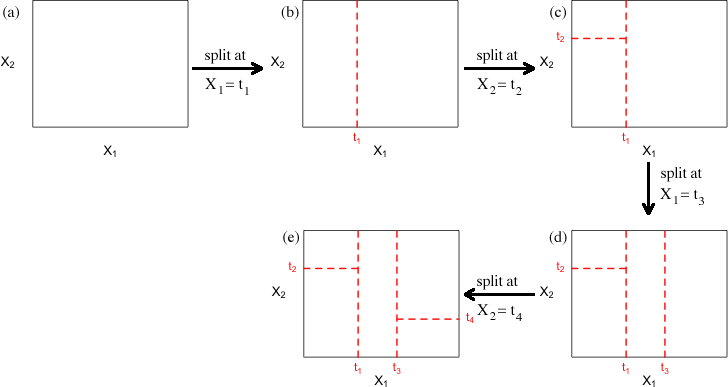
\includegraphics[width=1.0\textwidth]{fig/rec.png}}%
  \caption{���������� \tl{recursive partitioning} �� ��� \tl{predictors}}
  \label{figure:2}
\end{figure}

\begin{figure}[!ht] \center\leavevmode
%\epsfxsize=12cm \epsfysize=14cm
\epsfbox{fig/rec2.png} \caption{�������� ��� ������� $\tl{X}_{1}$, $\tl{X}_{2}$ ���� ��� \tl{recursive partition}}\label{figure:3}
\end{figure}

\begin{figure}[!ht] \center\leavevmode
%\epsfxsize=12cm \epsfysize=14cm
\epsfbox{fig/rec3.png} \caption{������� ������ ���� ��� \tl{recursive partition}}\label{figure:4}
\end{figure}

�� \tl{I} ����� ���� ������� ��� ������� �� � ���������� �������� �� ������ �������� ��������� �������. ������ ��� ���������� ������ �� ������ ���� ���� �� ���� ��� ��� ��� ����� �����������, �������� ��� ���� ����� ����� ��� ����������� �� ����� ���������. �� ���������� ��������� �� $\overline{y}$ ��� �������� ��� ������ �� ������������ ������.
\newpage
�� ���� ������� ������ �� ������������� �� ������, ���� �� ���� ���������� ����� �������� �� ������������ ���� �������� ��� ����� ����������� ��� ����. �� ������������ ��� ����������� ��� ������� ���������� ���� �������� ����� ��� �� ��������� ���� �����. � ���� ������� $\tl{R}_{i}$ ����� �� ����� ��� ������� ��� ������ �� ������ ������������ ���� ������� �� ��� ����������� ��������. �� ������ ����������� ����������� \tl{splits}. �� ������ ����������� ��� �������� ������� ����� � ������� �������� ���� ����� ��� �� ������ �� ������ ������������ ���������� \citepri{breiman1984classification}. ��� ���������� ��� ������� ��� ������������ ������������� �������� ���� ������ \ref{figure:4}.
\section{������ �����������}

\begin{figure}
  \makebox[\textwidth][c]{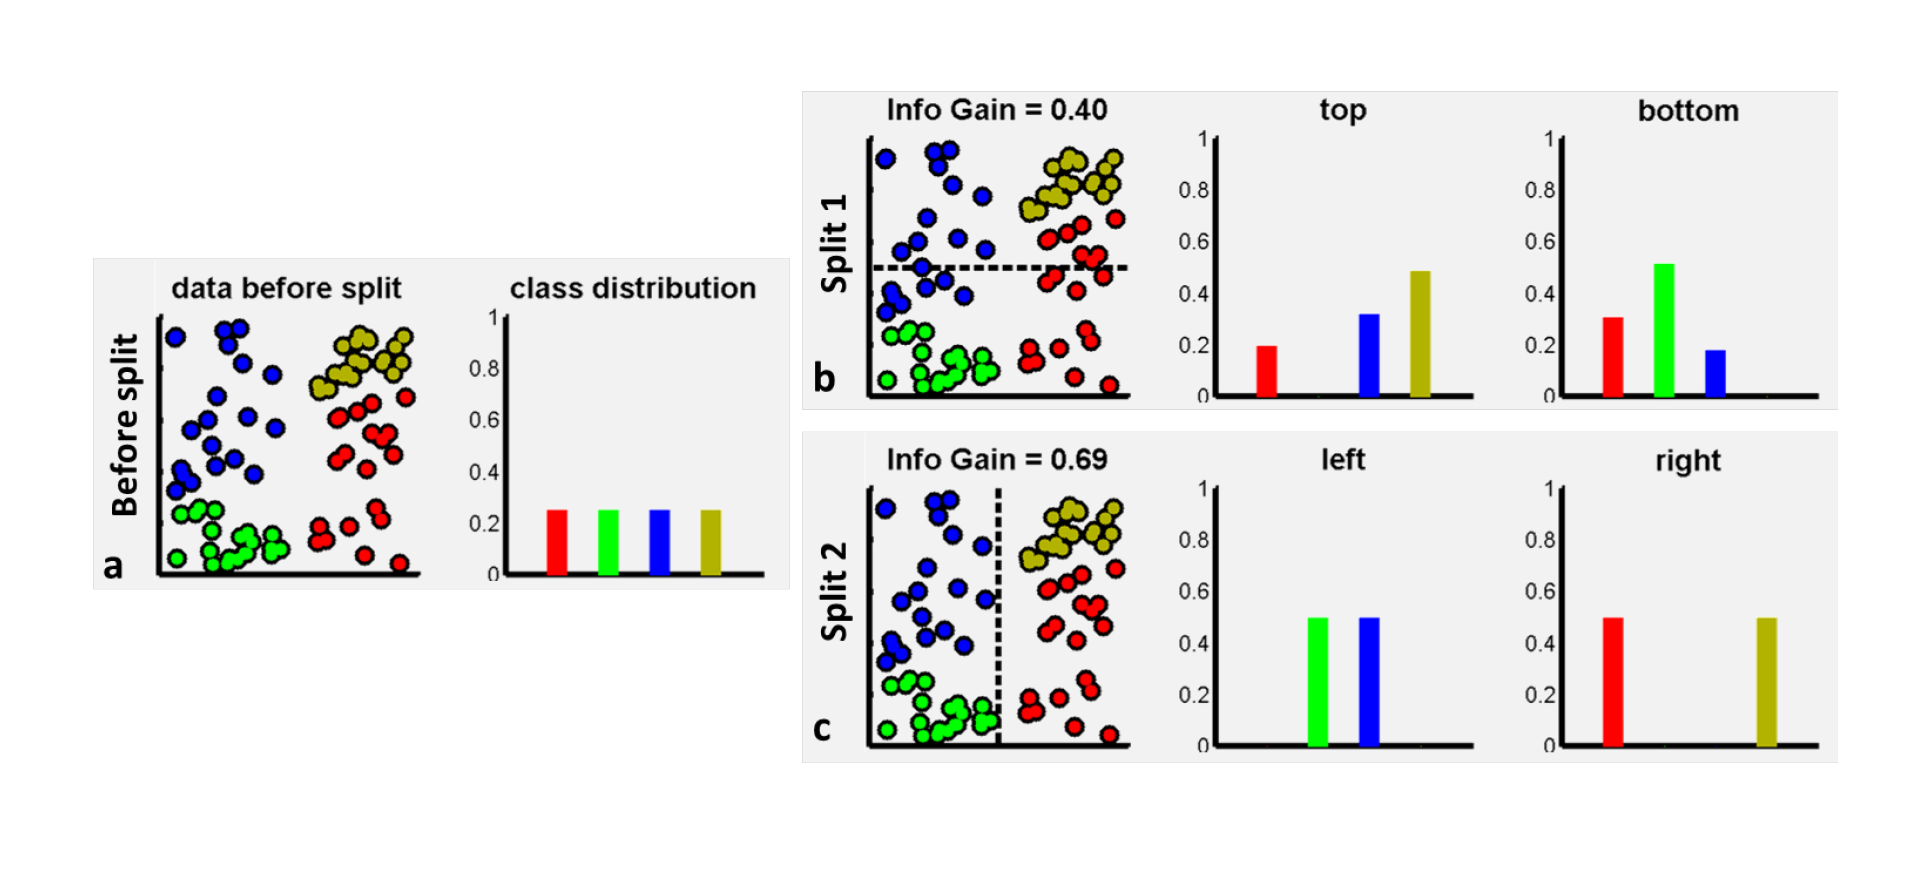
\includegraphics[width=1.2\textwidth]{fig/infogain.png}}%
  \caption{������ ����������� �� �������� ��������. (\tl{a}) ������ ������ ��������� $S$. (\tl{b}) ���� ��� ��������� ����������. (\tl{c}) ���� ��� ���������� ����������.  }
  \label{figure:-1}
\end{figure}

���� ��������� ��� ��� ��������� �����������, ����� ��������� �� ������������� �� ��� ������� ��� ��������� ��� ��� ������� ����������� (\tl{information gain}), �� ������ ���������������� ����� ���� ���������� ��� ��� ������ �����������. �� ����� \ref{figure:-1} ��� ������� ��� ������ ��������� ���� 2\tl{D} ����. ����������� ������� �������� ������������ �������. ��� ����� \ref{figure:-1}\tl{a} � �������� ��� ������� ����� ���������� ����� ������ ������� ��� ���� ������ ������� �� ���� �����. �� ����������� �� �������� ��� ��������� ���� ��� ����� \ref{figure:-1}\tl{b} ���� ��������� ��� ������ ���������. ���� ��������� ��� ������������� ���� ���������� ��������, ���� ������ ������������ ����������� �� ��������� ������������.
\newpage
�� ������ ����������� ��� ������ �� �� �� ����������� �� �������� ����� \citepri{deng2011bias}:
\begin{equation}
I = H(S)-\sum_{i\in\left \{ 1,2 \right \}}\frac{\left | S^i \right |}{\left | S \right |}H(S^i)
\end{equation}
�� ��� �������� \tl{Shannon} �� �������� �� (\citealpsec{shannon}):
\begin{equation}
H(S)=-\sum_{c\in C}p(c)\log (p(c))
\end{equation}
�� $S^i$ ����������� ��������� ��� ������� ���������, �� ����� ����� ������������ ���� ��� \tl{split} ��� ����� ������ �� ������ ����� $i$ ������������ ������� ������������ ��� ������� ��� ��������� ������ ��� �� \tl{split}.

��� ���������� ���, ���� ��������� \tl{split} ��� ���������� ���� ���� �� �������� ���, ��� ���� �� ���������� ��� ������ $I=0.4$. �� ���� ������������ �� �������� ������, ���� ��� ����� \ref{figure:-1}\tl{c}, ���� ������ ���� �������� ������������ �� ��������� �������� ��� ���������� ������ ����������� ($I=0.69$). ���� ��������� ����� �� ��� ������ ���������� ������ ������� ��� ��������� ��� �� ������ ���� ���� 2 �������, ��� ���� ����������� ��������� ���� ��� ������� ������. �� ���� �� ����������, �������� �� ����� ��� �������� �� ���������������� �� \tl{information gain} ���� �� ��������� ��� �������� ��� �� ��� ����� �� �������� ������������. � ������ ��� ������� ����������� �������� ��� ��� ���� ��� ������� \tl{random forest} ��� ����� �� ���������� ��� �������� 4. 

\section{���������� �����������}

�� ������ ��� ����������� ���� ��� ��������� ��� ������� ����� �� ���� �� ��������� ������������� � ����������� �� ��������������� �� ������������ ������ ��� ������� ��� ����� �������� ��� ���������� ���� ��� �� �������� �����������. � ���������� ���� �� ����: \\

\textbf{���� 1: ������� ���������� ��� ������� �����������} \hfill \\

\textbf{\tl{Regression}}: �� ��������� ��������� ���������� $m$ �� ��������� ����� $\xi_{1},\xi_{2},\dots,\xi_{m}$ ���������� ���� ��������� ���������. ��� ���� ��������� �������������� ��� ������ �����: $\left \{ x \leq \xi_{i} \right \}$ ��� $\left \{ x > \xi_{i} \right \}$, $i=1,2,\dots,m$. ���������� ���������� ���� ������ ���������� ����� ��� ���������. �������� ����������� $m-1$ ���������. 

\textbf{\tl{Classification}}: �� ��������� ��������� ���������� �� $m$ ���������� ������ �� ���������� ����� ���� �������� ������� �������� ��� ���������� �� ��� ������. �� ������ ����������� ������ �� ���������� ���������� ��� ��� ��������� ������ �� �������� �� ����������� ������. �������� $2^{m-1}-1$ ������ �� ���� ������� ������ �� ������ ����. \\

\textbf{���� 2: ����������� ��������� ����������� ���� ������� ���������} \hfill \\

\textbf{\tl{Regression}}: ���� ��� ������ ����� $y$ ��� ���������� ��� ��������� $X_{j}$ ��� �� ������ ����������� $s$ ����� ��������� �� ���� ��� ������: \begin{equation}
R_{1}(j,s)=\left \{ x | x_{j} \leq  s \right \} , R_{2}(j,s)=\left \{ x | x_{j} >  s \right \}
\end{equation}
��� �������� ���������� � ������� ������� ��� ��������������� ����� �� ������������ �������� ���������� (\tl{residual sum of squares - RSS}). ���� ����������� �� ��������, ������������ �� �������� ������������ �������� ���������� ��������������� ��� ���� ���� ���� ��� ���������� \citepri{berk2008statistical}.
\begin{equation}
RSS_{0}=\sum (y_{i}-\overline{y})^2
\end{equation}
��� ��� ������������ ��� ���������� ���� ���� ����� ������� ��� ���� ���� ��� ���������. ���� �� \tl{RSS} �� �����: \begin{equation}
RSS(split)=RSS_{1}+RSS_{2}=\sum_{R_{1}}(y_{i}-\overline{y}_{1})^2 + \sum_{R_{2}}{(y_{i}-\overline{y}_{2})^2}
\end{equation}
� ��������� $X_{j}$ ��� �� ������ ����������� $s$ ��� �� ������� �� �����������:
\begin{equation}
\max [RSS_{0}-RSS(split)]
\end{equation}

\textbf{\tl{Classification}}: ��� ������ ����������� �������� �����������. ���� $y$ ��� �������������� ��������� �� $m$ ���������� ��� ����:
\begin{center}
$n_{ik}=$ ������� ������������ ����� $k$ ���� ����� $i$ \\
$p_{ik}=$ ������� ������������ ����� $k$ ���� ����� $i$ 
\end{center}

���� �������� �� ���������������� ������ ��� �� ������� ��������:

\begin{enumerate}
\item \tl{Deviance}: \begin{equation} D_{i}=-2\sum_{k}n_{ik}\log p_{ik} \end{equation}
\item \tl{Cross-entropy}: \begin{equation} D_{i}=-2\sum_{k}p_{ik}\log p_{ik} \end{equation}
\item \tl{Gini index}: \begin{equation} D_{i}=1-\sum_{k}p_{ik}^2 \end{equation}
\item \tl{Misclassification error}: \begin{equation} D_{i}=1-p_{ik(i)} \end{equation}
���� $k(i)$ ����� � ��������� ���� ����� $i$ �� ��� ���������� ������ ������������.
\end{enumerate}

�� ������ ��� ������ ���������� ���� ������� ����� �� �������� ��� ��������� ���� �� ����� ���� �������: $\sum_{i}D_{i}$. ��� ���� ��� ��� �� �������� �������� �� ������ ���������������� ���� ���� �� ������������ ��� ������ ����� ����� ��� ����� �����. ������ ��� ������� ����� �� ���������� �� ������ �� ������ ����� ���� �� ������ ������ �� ����� ��� ����� �� ����� �� ���� ��� ���������� \citepri{recpartition}. 

�� ������� \tl{cross-entropy, deviance} ��� \tl{gini index} ���� ��� ��� ����� ������������ ����� ��� �������� ��� ���������� ��������������. �����������, ����� ��� ���������� �� ��������� ����������� ��� ������ �� ����� �� �� \tl{missclassification rate}.  \\

\textbf{���� 3: �������� ����������� ��� �������} \hfill \\

������� ���������� �������� �� ������ ��� ��� ����������� ������, ������� ���� ����� �� ������������ ������ ��� �� ������ ��� �������������� ����������, ����������� ����� ����� ���� �������� ������� ���� ��������. ������� ������������ �� ����������� ������� ��� ������ ��� �������������� ��� �� ����������� ������ ���� ������ �� ��������� �� ������ ���. \\

\textbf{���� 4: �������� ��� �����������} \hfill \\

���� ��� �������� ���������, �� ������ ������  ��������� ��� �������� ���������� ��� ������� ����� ���� ��������� ���������� �� ������ ��� ������������.

\section{\tl{Cost Complexity Pruning}}

� ���������� ��� ����������� ����� �������� ��� ������� �� �������� ������ ����������� ��� �� ������ ������� ���� ����� ���� �� �������� ����� ������ �������� ������� ��� ��� ������� ����. ��� ����������, �� ���������� �� ������ ��� ������ ����������� ��� �� ��� ����� ���� ���� ������ ���� ��� ��������, ���� �� ������ ������� ���� �� ����� ��� ���� ������ ����������� �� ��������� �������� ������ ��� ���� �������� �������. �������� ��� ���������� ��� �� ������� �������� ���� �� � ������ ��� ��������� ��������� ������� ������ ������� $\varepsilon$ ��� ����� ����, ���� ������ �� ������ ������� ���� �� ������ ��� ���� ���� \tl{split} ��� �� �������� ���������� ���������� ���������.

� ���������� ��� ���������� ����� �� ����������� ��� ���� ������ ������ $T_{0}$ ����������� ��� ���������� ��������� ���� ���� ���� ��������� ������� ������ ���������� ��� ������ �� ���������� �� ������ ������� �� �� �������� \tl{cost complexity}.

���� ��������� $T \subset T_{0}$ �� ����� ��������� �� ���������� �� $T_{0}$. ���� �� ����� ��� ������� $n$, ���� ���� ������ $n$ ������ ���� ������� $R_{m}$. ���� $\mid T \mid$ � ������� ��� ������ ��� ������� $T$.  

���� ��� ����������� ��� ���� ������ ������ �� $n$ �����. ������� �� ��� ��������� ��� ������������ ��������, �� ���� ������ ��������� �� �������� ������, ����� �� ���������� �� ������ �������� �� �������������� �������� ������ ���������� ��������. ���� $T$ �� ������ ������ ��� $\mid T \mid$ �� ������ ��� ������� ����������� ��� �������. �� �������� \tl{cost complexity} �������� �� ����:
\begin{equation}
CC(T)=\sum_{terminal ~ nodes}D_{i}+\lambda \mid T \mid
\label{CCT}
\end{equation}
�� $D_{i}$ ����� �� �������� \tl{RSS} ��� \tl{regression} � ��� ��� �� �������� ��� ����������� ��� \tl{classification} �� ������ ����� $i$. � ���������� $\lambda\geq0$ ����� ��� ���������� ����������� (\tl{tuning parameter or penalty term}). ���� ��������� ���� ��� ��������� ���������� ������������ �������� ������ ��� ��� ��������� ��� ��� �� �������� ������. ������� ����� ��� ���������� ����� �� ���������� ��������� ������, ��� ���������� ��� ��������� �� $\lambda$. ��� $\lambda=0$ ������ �� ������ ��� ������. 

�� $\lambda$ ������ ���� �������� ���� ���� � ��������� $K$ ��� \tl{Akaike information criterion} (\tl{AIC}), �� ����� ����� ��� ������� �������� ���� ����������� �������� ��� ������ ������ ��������� ��� ������� ���� ����� �������� ��� ������� �������� ������� �� �� \tl{fitting} ��� ��� ������������� ��� ������� �� ���������:

\begin{equation}
AIC=-2\log L+2K
\end{equation}

��� ���� ���� ��� ���������� $\lambda$ �������� �� �������� ��� ������� �������� �������� ��������� $T_{\lambda}$ ������ ���� �� ������������� ��� \ref{CCT}. ��� �� ������ �� $T_{\lambda}$ �������������� �� �������� \tl{weakest link pruning}: ���������� ��������� ��� ����� ��� ������� ��� ��������� ������ ��� $\sum_{n}D_{i}$ ����� �� �������� ���� ����. ���� � ���������� ��� ����� ��� ���������� ��� ��������� �� ����� ��������� �� $T_{\lambda}$ \citepri{quinlan1987simplifying}.

\section{\tl{Cross Validation}}

�������� ��� ���������� $\lambda$ ������ �� ���������� �� \tl{k-fold cross validation} (������� \tl{five} � \tl{tenfold}). �� ���� ��� ����� �������� �� ����������� ���� �� ������������ �� ���������� �� ������. 

��� ���� �������� ������ ��������� �������� � ��� ���� �������� ���� \tl{CC(T)} ������� \tl{k-fold cross validation}. ��� �� �� ��������� ����, ��������� ������ �� �������� ��� $D$ �� $k$-\tl{subsets} ���� �� ������:
\begin{center}
$D = D^{(1)} \cup D^{(2)} \cup \dots \cup D^{(k)}$
\end{center}
���� ���� �������� ��� ��� ��� �� $k$ ��������� $D_{i}$ ��� ��������� ��� ��������� ��� �� $k-1$ ��������� ���������� ���������� $\overline{y}_{i}$ � $\widehat{p}_{ij}$ ������� �� �� �� ������ \tl{regression} � \tl{classification tree}. �� �������� ��� ������ ��� ���������������� ��� �� ����������� �� ������. ���� � ���������� ������� $k$-����� ��� ���� ��������� ��� �� ������� ���� ������ \tl{xerror (relative average cross-validation error)} �����:
\begin{equation}
xerror = \frac{\frac{1}{k}\sum_{k}RSS(k-fold tree)}{RSS(null tree)}
\label{xerror}
\end{equation}
� ���������� ������ �� ���������� �� ������� ��� ���� ���������� ��� �������:
\textbf{������� 1}: ������� ��� ���� \tl{CC(T)} ��� ������� �� ������ �� ����� ������������� ��� \ref{xerror}. \\
\textbf{������� 2}: ���� $xstd$ � ������ �������� ��� ������� �� �� �������� $xerror$. ���� ������� ��� ����� (����������) ���� \tl{CC(T)} ������ ����:
\begin{equation}
xerror < \min (xerror)+xstd
\end{equation}

\section{������������}

�� ������ ��� ����� ������� ��� ����� ������ ���������, ����� ���� ��� �� ���������� ����������� ������ ������ �� ������� ������� ��������� ��� �� ������ ��� ������ ���� ��������� �������� �� �� �������� ���. ��� ��� ���� ������ ����� ���� ������� �� ������ ������ ��������� �� ������ ���������� ���� ������� ���� ������� �� ����� ���������� ����� �� ������ ��� ������� �� ����������� �� �� ������ ������� �������������. �� ����������, ������� �� ��� ������ ���� ����� ����������. ����� ��������� �� ����������� ��� ���� ��� ������ ����������� ���, �� ������ ��� ������ ��� ����� �������� �� �������� ����� ��� �� ��� �� ��������� ��� ����� ���������� �� �� �������� ����� ��� �� �������� ������� \tl{pruning} ���� � ������� \tl{cost complexity} ��� ������������ ����.

�� ����� �� �� �������� ����������� �������, �� ������ ������� �� ��������������� ��� �� ���������� ������� ��������������� ������ ����������. ��� ����������, ���� ��� ������������ ���������� ���������������� ��� �� ���������� �� ������ �� ����������� ������ ���� ���� �����, ���� �� �������� �� ���������� �� ��� ������������� ������ ����� ��� ��� ����������. �����������, �� ��� ��������� ����������� ������ ����� ���� ����� ��� ����� ������, ���� ���������� ��� ������ �� ������� ��� �� �������� ����� ������ ����� ��� ���������� ��� ��� ������ ��� ����������. �� ������ �� ���������� ����� �� �� ���������������� ���� �� ����� �� ������� ������ �������� ���� ��� ���� �� ���� �������� ��� �� �������� ����������� ������� \citepri{fielding1999machine}. 

�� ������ ����� �������� ������� ����������. �������� ������� ���� ����� ���� ��������� \tl{ensemble methods}, �� ������ ������������� �������� ���� \tl{boosting, bagging} ��� \tl{random forests}. � ���� ���� ��� ����� ��� �������� ����� �� �������������� ������ �� ��������� �������� ���������, ��� �� ������� ��� ���� ��� ��� ���������� ����� ������ ��� ���������� ����������� \citepri{frayman2002solving}.

\newpage
\thispagestyle{empty}
\chapter{\tl{MARS} }

\section{��������}

�� \tl{MARS} (\tl{Multivariate Adaptive Regression Splines}) ����� ��� ������������� ������� ������������� ��� ����� ��������� ��� ������ ���������� ���������� �� ����� ��������� ������ ������ �������. �� \tl{MARS} ������ �� �������� �� ��� ��������� ��� �������� ��� ��������� ������������ ������������� ��� �� �������� ������������� � �� ��� ����������� ��� ������� \tl{CART} ���� �� ��������� ��� ��������� ��� ���������� ��� ������� ��� ������������� (\citealpsec{mars_example}).

�� \tl{MARS} ������������� ��� ��� \tl{Jerome Friedman} �� 1991. � ���� '\tl{MARS}' ����� �������� ���� ��� �������� \tl{Salford Systems} ��� ��� \tl{open source implementations} ����� �� ����� '\tl{earth}'. ��������� ���������� �� ����� �� ���� ������� ���� \tl{random forests} � \tl{neural networks}. ������ �� ��������� ��� ������� \tl{MARS} ��� ������ �� ������� ��� ������� �� ���� ������� ���� �� \tl{CART}. 

\section{\tl{MARS} ��� \tl{Normal Regression}}

��� ����� \ref{figure:5} �������� ��� �������� ����������� ��� ����� �������� ���� ��� �������� ���� ����� �������� \tl{MARS} ��� ���� �������� ��������� ������������� ���� ��� ���� ��������. ������ ����������� ��� ��� ������� ��� ������������� ������ ��� �������� ��������� � ����� ���� �������������� ���� ��� ������ ��� ��������� ��� ����� ��� �� ����� ����. ��������, ��� ������� \tl{MARS} ������ ������� �� �������� ��� �� �������� ��� ������ ���� ��� �������� ��������� ��� ���� �������, � ����� ���������� �������� �� �������� ��� ���� ���� ������������ ������� �� ����� �� �� ������� ��� �������������. �� ���� ��� ����� ������������ �������� ��� ��� ������ ������������. 
\newpage
�� �������������� ���� ��������� ������������ �������� (\tl{Global Parametric Model}) ���� ��� ���������� � �������� ������������ ����� �� �������� (\citealpsec{mars_train}):
\begin{itemize}
  \item ����� �������� ����������� ���� �� ������������ ��������
  \item ������� ���� �� �� ������������ ������� ���� ��� ����� ����������� ���� (��� ���������� ����������� ������������)
  \item ���������� ���� �� ����� ������ ���������
  \item ��� �� �������� �������� �������� ���� ��������� ��� ������� ��������
\end{itemize}

\begin{figure}
  \makebox[\textwidth][c]{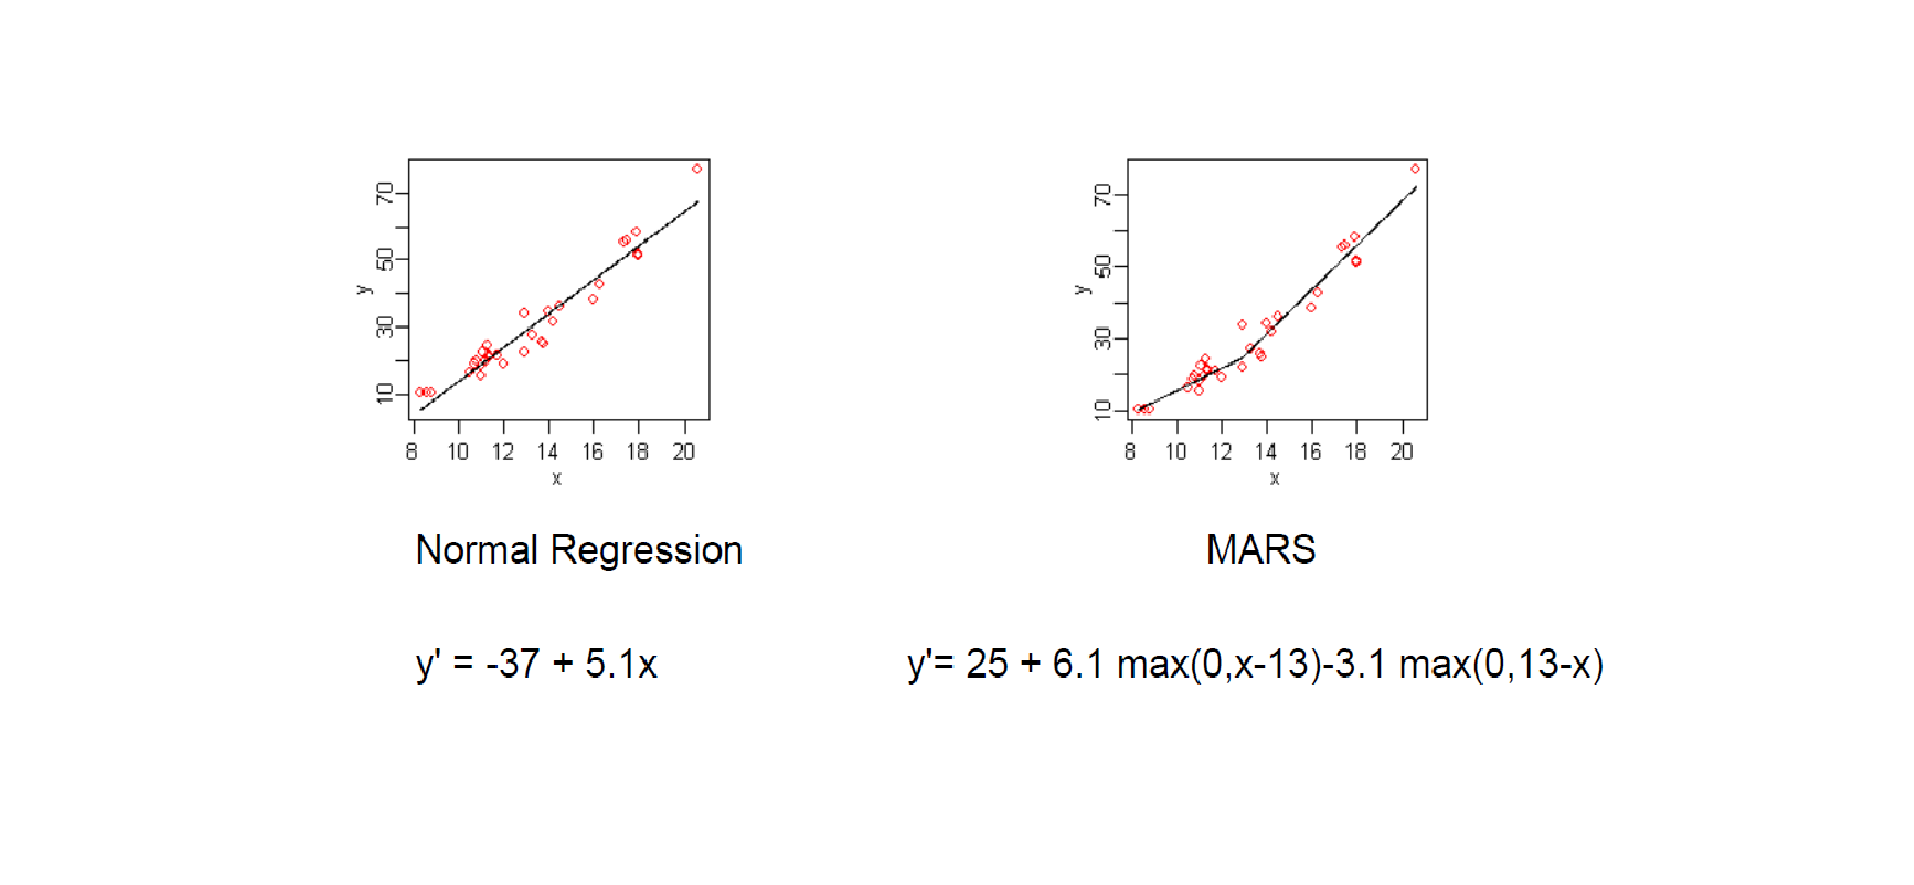
\includegraphics[width=1.5\textwidth]{fig/Untitled2.png}}%
  \caption{\tl{MARS} ��� \tl{Linear Regression}}
  \label{figure:5}
\end{figure}

��� �� ����������� ������� �� �������� �� ���� ���������� ��� ������ ��������� ������ ��� ��� ��������. �� �������������� ��� ����� �� ����:
\begin{itemize}
\item ������������ ��� ����� ������� ��� ���������
\item ��������� ��� �� ���������� ��������������� ���� ������������ �������
\item ���������� ��� ��������� ������� �� ���� ������� 
\item ���� ��� ���������� �� ��������� ������������ ���������
\end{itemize}

\section{��������� ��� �������}

�� \tl{MARS} ����� ��� �� ����������� ���������� ������������� � ����� ��� ����� ����� ������� ������� �� ��� ���������� ����� ������ ��� ����������� ��� ��� ����������� ���������� ��� ����������. �������� �� ����������� ��� �� ����������� ���������� ���� ��� �� �������� ���. ��� ��� ������, � ������� ��������� ���� ������� ''������� ��� ��������'' (\tl{Divide and Conquer}) � ����� ���������� ��� ���� ������� �� ��������, ���� ��� �� ��� ���� ��� ������� �������������. �� ������� ���� ������� �� 
\tl{MARS} ��������� ��� ���������� �� ���������� ���������� ������� (������ �� ������������ ��� 2 ����������) ���� ����� ��������� �������� ��� �� ����������� ���� ����������� (\citealpsec{mars_ref}).

�� \tl{MARS} ������������ ��������� ��������� ����������� ��� ������ $(x-t)_+$ ��� $(t-x)_+$ �� ������ ����������� ''����������� ����� ''. �� ''+'' �������� ��� ���������� ��' ��� ��� ���� �� ������ ����� ��� �����������, ������ �������� ��� ��������� ��������. ������ �������� \citepri{friedman1995introduction}: \\
\begin{center}
$
(x-t)_+ = \begin{cases}
x-t, & \text{�� $x > t$,}\\
0, & \text{�����������}\\
\end{cases}
$
~,~
$
(t-x)_+ = \begin{cases}
t-x, & \text{�� $x < t$,}\\
0, & \text{�����������}\\
\end{cases}
$

\end{center}

\begin{figure}
  \makebox[\textwidth][c]{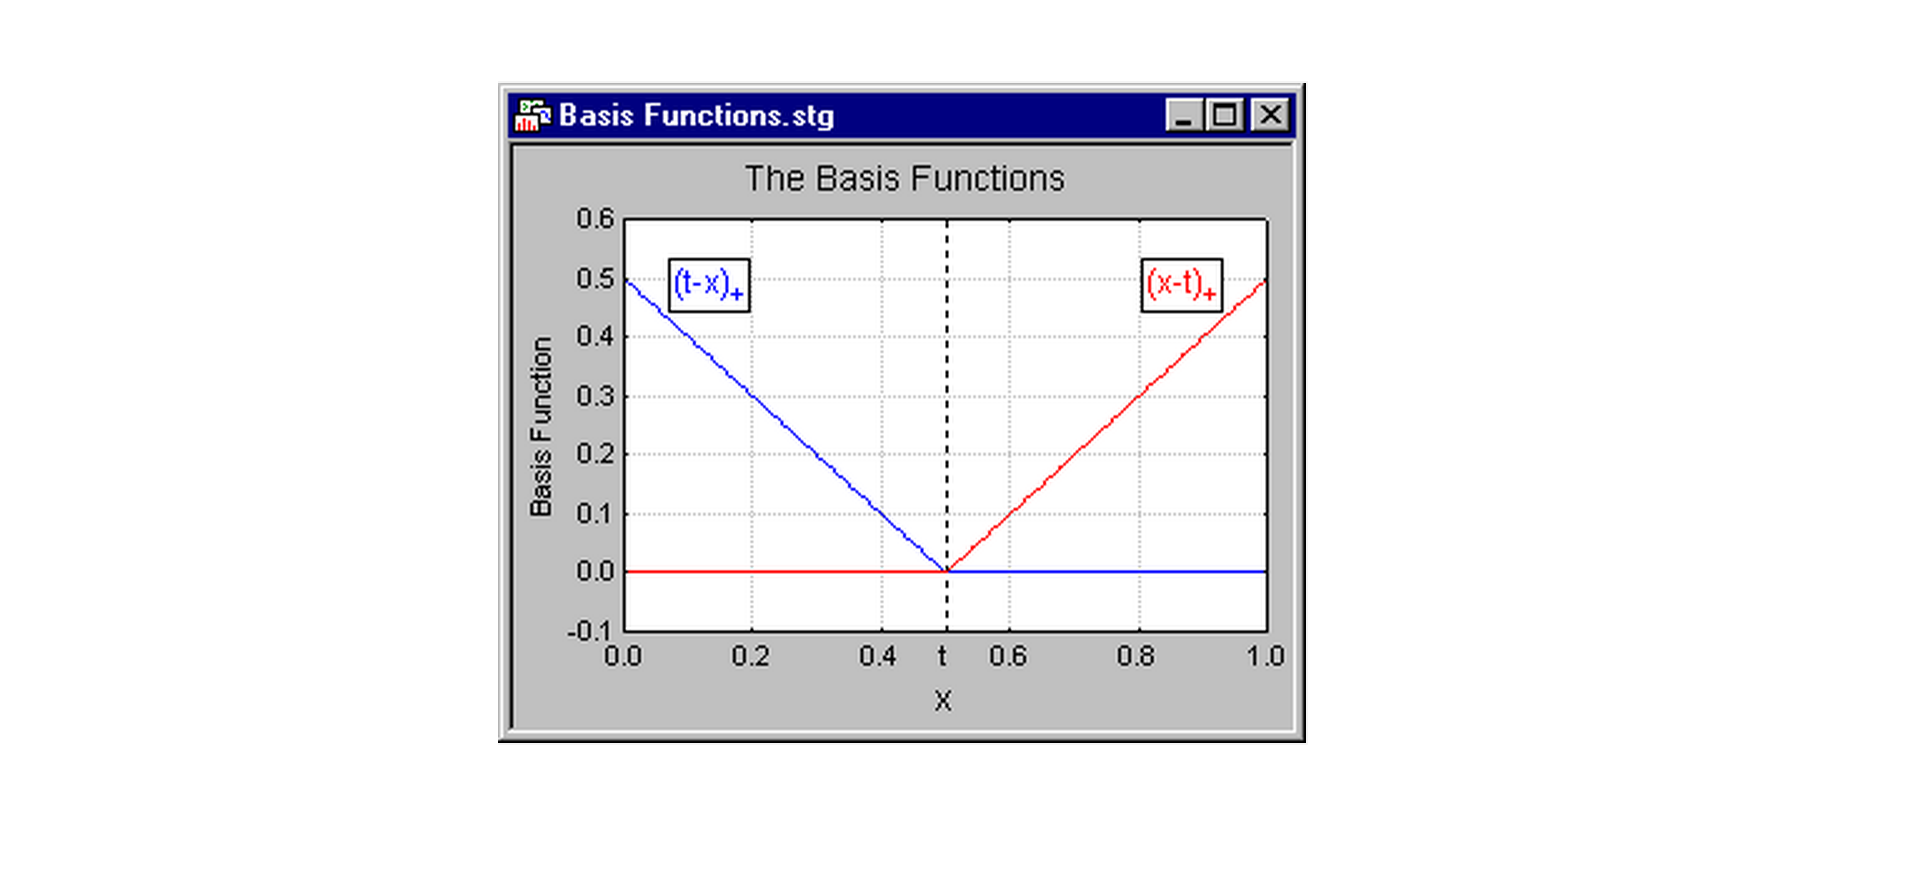
\includegraphics[width=1.5\textwidth]{fig/basis_fun2.png}}%
  \caption{�� ����������� ����� $(x-t)_+$ ��� $(t-x)_+$ ��� \tl{MARS}}
  \label{figure:6}
\end{figure}

��� ����� \ref{figure:6} ������ ��� ���������� ��� ����������� $(x-0.5)_+$ ��� $(0.5-x)_+$.

�� ����������� ����� ��������� ���������, �� ����� (\tl{knot}) ��� ������ $t$ ��� ����������� \tl{linear splines}. �� ��� �����������  $(x-t)_+$ ��� $(t-x)_+$ ��������� ��� \tl{reflected pair}. � ���� ����� �� �������������� \tl{reflected pairs} ��� ���� ������ $X_{j}$ �� \tl{knots} �� ���� ������������� ���� $x_{ij}$ ��� ������������� �������. �������� �� ������� �������� ��� ����������� ������ ��� ���� ������ �� ������:
\begin{equation}
C =\left \{ (X_{j}-t)_{+},(t-X_{j})_{+} \right \}_{\begin{matrix}
t\in\left \{ x_{1j},x_{2j},\dots,x_{Nj}  \right \}
\\ 
j=1,2,\dots,p.
\end{matrix}
}
\end{equation} 
�� ���� ���� ������� ����� ����������� ���� �� ������ �������� $2Np$ ����������� �����. ������ ���� ��������� ����� ��������� ���� ��� ��� ������������ $X_{j}$, ��� ���������� $h(X)=(X_{j}-t)_{+}$, ��������� ��������� ��������� ��� ����� ������� $\mathbb{R}^{p}$.

�� ����������� ����� ��� ������� $C$ ���� �� �� �������� ���� ������������ ��� �� �������� ���������� ��������� ��� �������. � ������ ��������� ��� �������� \tl{MARS} ����� \citepri{friedman1991multivariate}:
\begin{equation}
f(X)=\beta _{0} + \sum_{m=1}^{M}\beta _{m}h_{m}(X)
\label{eq2}
\end{equation}
���� ���� $h_{m}(X)$ ����� ��� ��������� ��� $C$, � �� �������� ��� � ������������ ������� �����������.

��������� ��� $h_{m}$, �� ����������� $\beta _{m}$ ������������� �� ��� �������������� ��� ������������� ����������� ���������� ���� ���� �������� �������� ������������. ��� ��� ��������� ��� ����������� $h_{m}(X)$ ��������� ��� ��� ������� ��������� $h_{0}(X)=1$ ��� �� ���� ��� ����������� ��� $C$ �� ���������. �� ���� ������ �������� �� ��� ��������� ������� ����������� �� �������� ���� ���������� $h_{m}$ ��� ������ $M$ �� ��� ��� �� \tl{reflected pairs} ��� $C$. ����������� ��� ������� $M$ ��� ��� ��� ������:
\begin{center}
$\widehat{\beta}_{M+1}h_{l}(X)\cdot (X_{j}-t)_{+}+\widehat{\beta}_{M+2}h_{l}(X)\cdot (t-X_{j})_{+}, h_{l}\in M$
\end{center}
� ������ ���������� ��� ���������� ������ ���������. �� ���� $\widehat{\beta}_{M+1}$ ��� $\widehat{\beta}_{M+2}$ ������������� ��� �� �������� ��������� ���� �� ���� ���������� $M+1$ ����� ��� ��������. ������ �� �������� �������� �������� ��� ������� $M$ ��� � ���������� ����������� ����� �� ������� $M$ �� ���� ������ ������� ������ ����.

\begin{figure}
  \makebox[\textwidth][c]{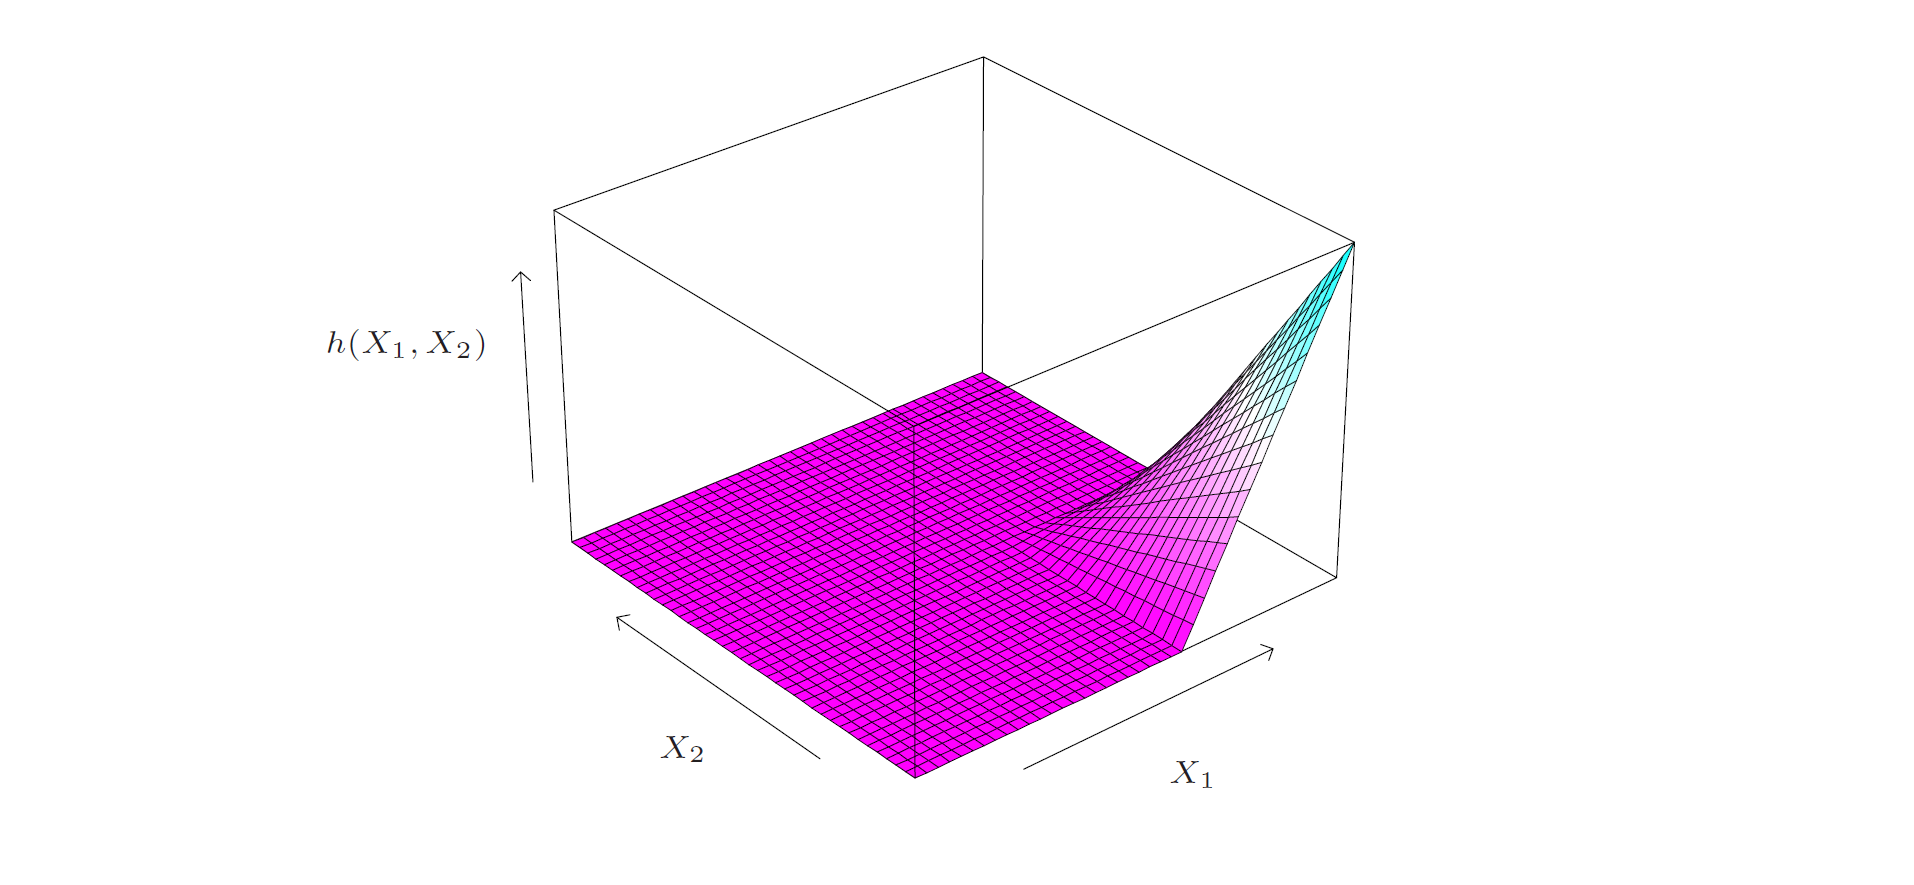
\includegraphics[width=1\textwidth]{fig/mars_ex.png}}%
  \caption{���������� ���������� �� �������� ����������� �����}
  \label{figure:7}
\end{figure}

��� ����������, ��� ����� ������ ��������� ��� ������� ��� ��������� ��� ������ $\beta _{1}(X_{j}-t)_{+}+\beta _{2}(t-X_{j})_{+};t \in \left \{ x_{ij} \right \}$ ������ �� �������� �� ��� ������� ��������� $h_{0}(X)=1$ ��� ����� ��� ���� ���������. ���� � �������� ������� ������� �� �� ����������� ��� ����� � $\beta _{1}(X_{2}-x_{72})_{+}+\beta _{2}(x_{72}-X_{2})_{+}$. 
\newpage 
���� �� ������� ����������� ������� ��� ������ $M$ ��� ��� ������� ���� �������� ��� ������� ��� ������: 
\begin{center}
$h_{m}(X)\cdot(X_{j}-t)_{+}$ ~ ��� ~ $h_{m}(X)\cdot(t-X_{j})_{+}$, $t \in \left \{ x_{ij} \right \}$
\end{center}
���� ��� �� $h_{m}$ ������ ��� ���� ��������:
\begin{center}$
\begin{matrix}
h_{0}(X) & = & 1,\\ 
h_{1}(X)& = & (X_{2}-x_{72})_{+}, \\ 
h_{2}(X) & = & (x_{72}-X_{2})_{+}
\end{matrix}$
\end{center}
� ����� ������� ���������� ����������� ���� � $(X_{1}-x_{51})_{+}\cdot(x_{72}-X_{2})_{+}$ ��� �������� ��� ����� \ref{figure:7}. 

\section{\tl{Generalized Cross Validation}}

��� ����� ��� ����������� ������ ��� ������ ������� ��� ������ (\ref{eq2}). �� ������� ���� ���� ������������ ����������� ����� \tl{overfit} �� ��������, ����� ������������ ��� ���������� ���������� ��������� (�������� �� ��� ���������� ���������� ��� ������ ��� \tl{classification trees}) ���� ��� ����� �� ���� ���� � ���� � ������ ���������� ��� ��������� ������ ��� ������������� ������������ ��������� ����������� ��� �� �������. �� ���������� ��������� ��� ���������� �������� ������� $\widehat{f}_{\lambda}$ ��� ������� (������ ����) $\lambda$. ��� ��� ������ ��� ��������� ����� $\lambda$ �� ���������� �� ���������������� \tl{cross-validation}, ���� ��� ������ ������������� ������� �� \tl{MARS} ������������ �� �������� \tl{generalized cross-validation}.
\newpage
�� \tl{generalized cross-validation} �������� ��:
\begin{equation}
GCV(\lambda) = \frac{\sum_{i=1}^{N}(y_{i}-\widehat{f}_{\lambda}(x_{i}))^2}{(1-M(\lambda)/N)^2}
\end{equation}
� ���� $M(\lambda)$ ����� � ������� ��� ���������� ��� �������� �� ����: ���� �������������� ���� ��� ������ ��� ���� ��� �������� ���� ��� ��� ������ ��� ���������� ��� ���������������� ��� ��� ������� ��� ��������� ������ ��� \tl{knots}. ������� ����������� ������������� ������������ ��� ����������� ������� ����� ���������� ��� �� ��������� ��� \tl{knot} �� ��� ��������� �������� ������������. �������� �� �������� $r$ ����������� ��������� ����������� ����� ��� �������, ��� $K$ \tl{knots} ����� �������� ���� ��� �������� ��� �����������, �� ������: $M(\lambda)=r+cK$ ���� $c=3$. ������� �� ����, ���������� �� ������� ��� ���� ��� ���������� ���������� ������������� �� $GCV(\lambda)$.

\section{� ���������� \tl{MARS} ���������}

���� ���������� ��� ���� �� \tl{MARS} ����� ��� ���������� ��� ������� � ����� ����������� ��������� ����� �� �������� ��� ������� �������. ��� ����� ������ ������������ �� ������� ������������ ����������� ����� ��� ���������� ��� ������������� ��� ����� �� �������� �� ��� ������������ ������ ��������������. ��� ������� ������, ��������� ''���� �� ����'' ��� ��������� ��� �������� ���������� ����������� ������� �� �� �������� \tl{Generalized Cross Validation}. � ���������� ���� �� ����:
\begin{enumerate}
\item ������ �� �� ���������� ������� ��� �������� ���� ��� ������� ��������� �����
\item ��������� ���� ���� ��� ����������� ����� ��� ��� ���� ��������� ��� ��� ��� �� ������ \tl{knots} �������� ��� ������� ��� ����������� ��� ������������� ������ �������� ������������ (\tl{goodness of fit}) ���� ��� ���������� �������������� ��������� ���������
\item �������� ���������� �� ���� 2 ��� ���� �� ������� ��������� ��� �������������� ������� �������������
\item ������� �� ������ ������������ ��� ������� ����������� ��� ���������� �� �������� (\tl{least squares}) ��� \tl{fitting} ��� �������� ���� �� �������� �� ������ �������.
\end{enumerate}
\newpage
\section{������������}
�� \tl{MARS} ���� ����� ���� ��������� ��� ��� ���������� �������� ��������� ��� ''�������'' ���������� �������� ���������, ��� ����� �� \tl{predictors} ��� ������������ ����� � ��������� ������� �� ��� ����������� ����������. ����������� ������� ��������� �� \tl{CHAID}, \tl{CART}, ���� ��� �� ��������� ������ (\tl{Neural Networks}) \citepri{lee2001review}. ���� ��� ������������� ������ �� ��� ����� �� \tl{MARS} �������� \tl{predictors} (����������� �����), ������ �������������� ���� �� ����������� ���� ������� ���� �� \tl{CART} ��������������� ����, ������ ���� ��������� ��������� ���������� ���������� ���� ���������� ������ �������� ����������. ���� ��������������, ���� �� �������� �� \tl{MARS} �� ��� ��������� ��� ��������� �������������, �������� �� ������������� �� \tl{MARS} �� ��� ��������� ��� \tl{regression trees} ���� �� ''������'' \tl{binary splits} ������� �� ��������������� ��� '' ������ '' ����������� ����� \citepri{munoz2004comparison}.

��� ��������� �������� ��� ����������� ����� ����� � ��������� ���� �� ����������� �� ������ �������. ���� �� ����������� ������ ����������������� ������ ���� ���� ��� ����� \ref{figure:7} ���� �� ���������� ����� �� �������� ���� �� ��� ����� ����� ��� �������� ��� ����� ��� �� ��� ����������� ����� �� ���������. �� ���������� � ��������� ���� ����� ������� � ������������ �������� ������ ���� �� ��������� ��������� ����� ���� �����������. � ����� ����� ����������� ����� ���� ��� ������������ ������� �� �������� �������� ��� ����� ���� ����, ����� ��� �� ������������ ����.

��� ������� ��������� ����������� ��� ����������� ����� ����� �� ������������ ������. ���� �� �������� ���� ���������� ��� $M$ �� ������ ��� �� $N$ \tl{reflected pairs} ��� ������ $X_{j}$. ���� �������� �� ������� �� ��������� $N$ ��������� �������� ������������� ����� ������� ������ ��� �� ����� ������������ $O(N)$ ������������ �� ���������� �� ������ ������������� $O(N^2)$. �� ���� �� ������ �������� �� ��������������� ��� ����� ��� ����������� �����. ������ ����������� �� ������ �� �� ��������� \tl{knot}. ����� �� \tl{knot} �������� ��������� ��� ���� ��������, �� ����������� ������ �� ��������� ���� ����� ��� �������� ����� ��� �������� ��� ���� ��� ������� ��� ���� �����. �������� �� ���� ���� �������� �� ������������ �� ������� �� $�(1)$ ����� �������� �� ����������� ���� ������ \tl{knot} �� $�(�)$ ������������.

�� ������� \tl{MARS} �������������� ���������, ���� �� ���� ����������� �������������� ��� �������� �� ����� ����������� �� ������ ����� ������������ ��� �������� ������������ ������� ��� ���������� ��� ��� �������. ��� ���������� ��� �������� �� 4 ����������� ������ �� ����� ���� �� �� �������� ��� ����� �� ��� ����������� ��������� ��� ��� �������. �������� ��� ������������� ������ ����� �� ������� ���� �� �� ��������� ���� ����� �������� ��� ��� �������. �� ���� ��� ����� ����������� �� ���������� ��������� ������ ��� ������� ���. �����, ������ ��� ���������� ���� ��� ���������� ��� ��������. ���� ������� ������ �� ���������� ����� ��� ���� ��� ��������. ���� ��������� ��� ���������� ����������� ����� �������� �������, ��� �� ��� ����������� ����� ��� ����� ��������� ��������� �������� �� �������������� ���� ���������� �� ��� ������� ����� \citepri{cart_mars}.

���� �� ������� ��� �� \tl{MARS} ������ ���� ������������ ��� ������� ����������� \tl{regression}, ������ ������ �� �������������� ��� ��� ���������� \tl{classification} ���� ��� ����������� ��� �������� �� ���������� ���������  ���������� ������. ������ ������������� ��� ������� ������ �� ���������� ������� (\tl{multiple indicator variables}). ��� ����������, �� ���������� �� ��������������� �� ''1'' ��� ���������� � ����� ������ ���� ����� $k$ ��� �� ''0'' ��� ���������� ��� ��� ������ ���� ����� $k$. ������ ����������� ��� ��������� \tl{MARS} ���� ��� ������� � ������ ��������� ��� ����� ������ ����������� ����� ��� ��� �������� ��� ���� �� ������������� ����������� ��� ���� ��������� ��� ��������� �� ���������� ������� ���������� �� �������� ����� � \tl{scores}. �����, ���������� ��� ����� ��� ������ �� ���������� \tl{score} ��� �������� ���. ����������� ��� ��� ���� � �������� �� ����� \tl{classifications} �� ��������� ����� ��� �� ������������ ���� ���� �����, ���� ��� ��������� �� ������ ���������� ������� ��� ������� ����������� ��� �� ���� ����� �� ���������� �� \tl{classification}.

\newpage
\thispagestyle{empty} 


\chapter{\tl{Random Forests} }

\section{��������}

�� \tl{random forests} ��������� ��� ������ ������� ��� ������ �� �������������� ���� ��� ���������� ����������� ��� ��� ��� ���������� �������������. ����������� �� �� �� ������������� ��� ������ ��� ������ �������� �� ������ ��� ������� ��� ��������� ���� �� ���� ����������� ��� �������� ��� ������ �� �������������� ��� �� ������ ��� �� ���������� ��� ������ �����. ��������� ��� ����������� ��� ������� \tl{bagging}, � ����� ������� ����� ���������� ������� �� ������ ��� ������� ��� ���� ���� �����, ���������� ��� ���������� ��� ������. 

�� ������ �������� ����� ��� ��������� ��� ��������� ��� �������� 2 ��� ����� �������� ��������� ��� �������� \tl{bagging} ����� ������� �� ��������� ���������� ��������������� ������ ��� ���������, ��� �� ���������� ������ �����, ����� ������� ������ ���������. �����������, ���� ��� ������� ��� �����, � ����� ���� ���� �������� ���� ���� ������ ��� ����������� ������. ���� ������ ��� ��������� ���� ��� ����� \tl{identically distributed}, ������ ����� ���������� ��� �� ���� ������ ��� ������� ��� ���� �������� ����������� �� ���� ��� ������ �����. �� ���� ��� �����, � ����� ���� ���� ��� ������� ������� ��� ���� ��������� �� ���� ��� ������� ��� ������ ��� ���� ���, ����� ������������ �������� ���� ������� ��� ����������� \citepri{clauset2011brief}.

\section{��������� ��� �������}

� ���������� ��� ������������ ����� ������ ���� �� ���� ��� ��������� ���. ���� ��� ���� \tl{split} ���������� ������ ������� ���������� ������� �� ��������� ��� ����������. ������, ��� ����� ��� ���������� ���������� �� \tl{split point} ��� �� ��� ����� �� ���������� ������ ����������� (���� �������� ��� �������� 2.2) ��� ��� ��������� ���� ����� �� ������� ��� ����������. ������ ������� �� \tl{split} ��� ��������� ��� ������� - ������ �� ������ ��� ������ ��� �������� ����������. � ���������� ���� ��������������� ���������� ��� ���� ������ ��� ��� ����� ����������� ������ ������. ��� ����� � ������ ��� ��������� ���� ��� ������ ��� ������� ��� �������� ��� ���� ��� ����.

\begin{figure}
  \makebox[\textwidth][c]{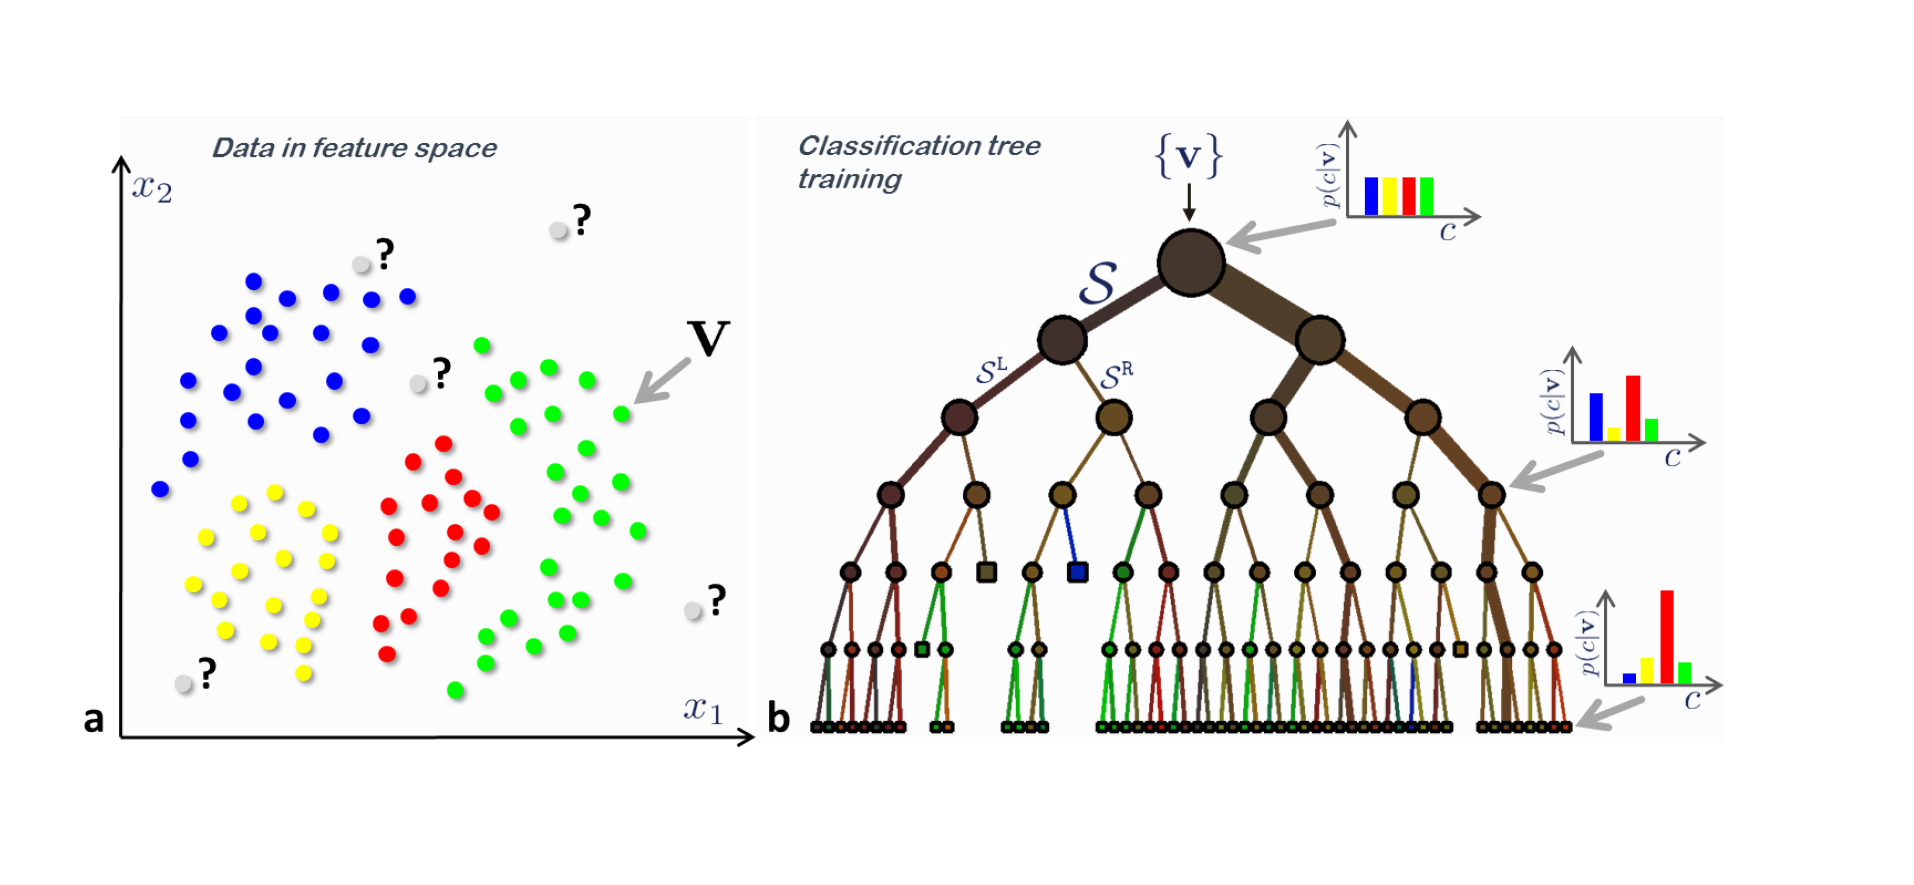
\includegraphics[width=1.2\textwidth]{fig/rand1.png}}%
  \caption{���������� ���� �������� �������}
  \label{figure:8}
\end{figure}

��� ����� \ref{figure:8} �������� ��� ���������� ����������� ���� \tl{random classification tree}. ������ ���������� ������ ������ �������� ��� �� ������ �����������, ��� ������ $V$-������ ��������� ���������������� ���� �� ���������������� ��� ����������� ��� �������. �� \tl{split points} ��� ��� ������ �� �������� ������ ����������� ���������������� ��� �� �������� ���� ������� ��� ������� �� ����� ������� $S^L$ ��� $S^R$. ����������� ��� ��� ���������� ��� ��� ����� ���� �� ����� � �������� ��� ��������� �������, ������ ��������� � ����������� �� ���� ��� �������� ��� ���������� �� �������. ��� ���������� � ��������� ���� ���� ������ ���������� �� ������ ���� ����� �� ������� �����, �� ������������� ��� �������� ��� ��� ���� ��� ����� $C$. ���� ������ ��� ���� ���� �� ���������� ����� ��� ���� �������� �����������.
\begin{figure}
  \makebox[\textwidth][c]{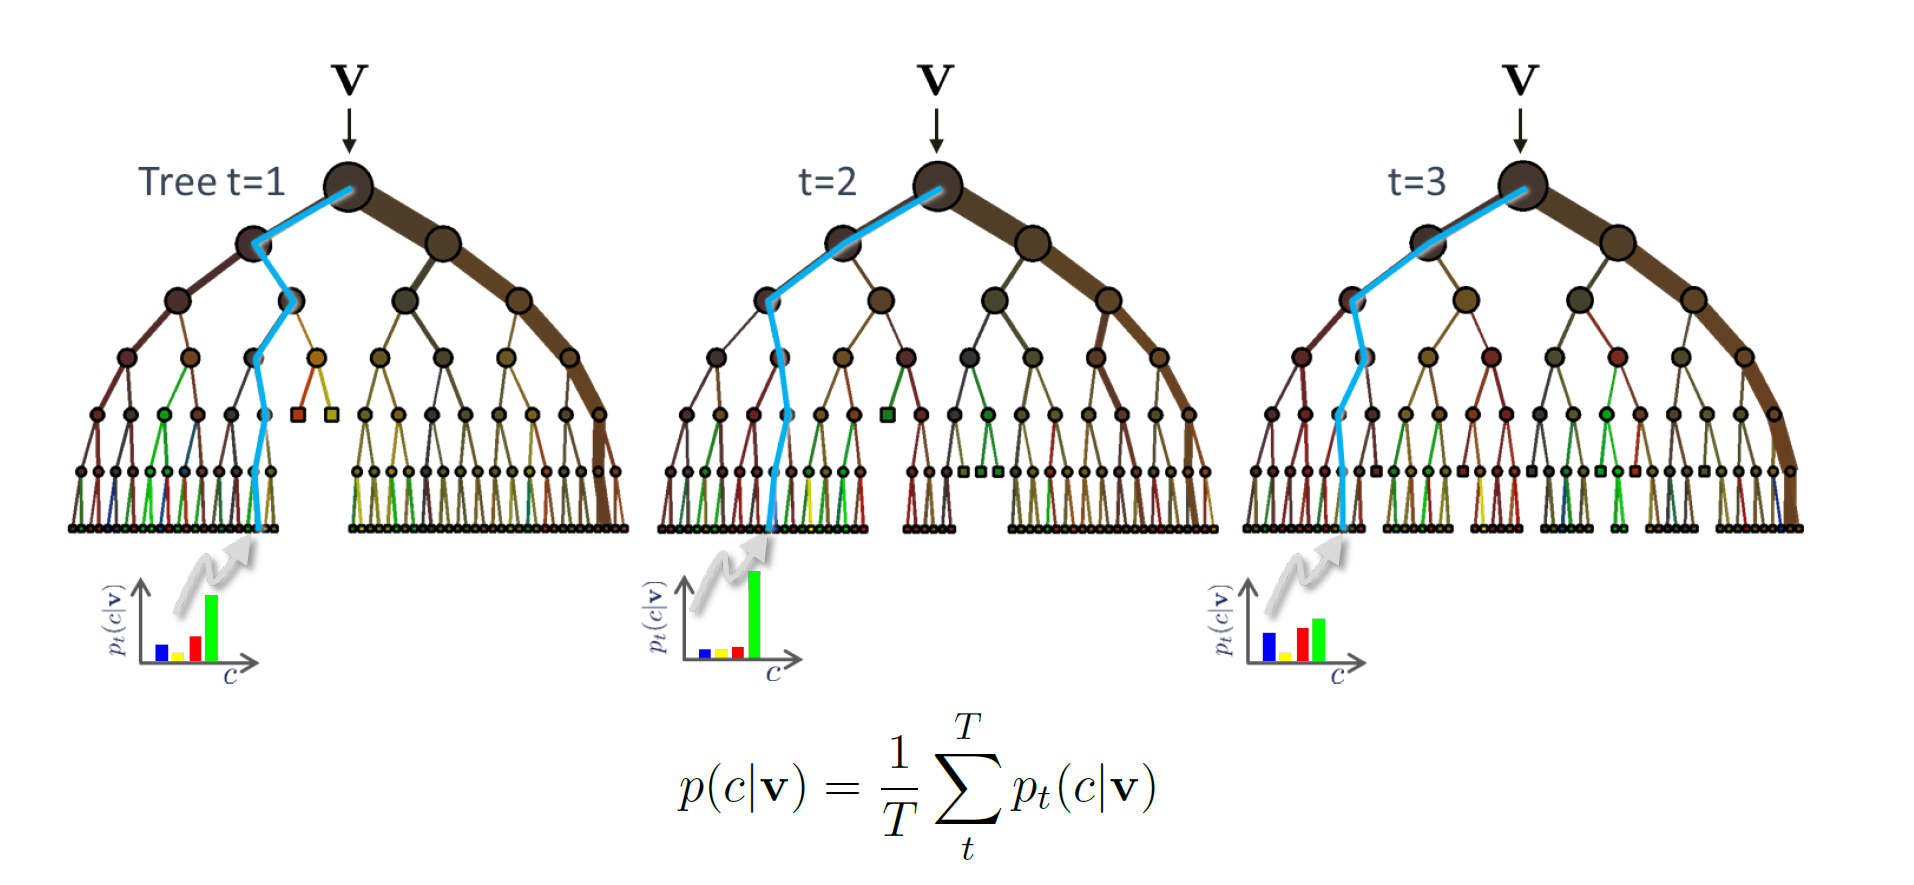
\includegraphics[width=1.2\textwidth]{fig/rand2.png}}%
  \caption{������ �� �� ������ (\tl{ensemble}) �����������}
  \label{figure:9}
\end{figure}

��� ����� \ref{figure:9} ������ ��� ���������� ����������� ������ ��� ������ ��� �� �������� ���, ���� $\mathbf{v}$. �� ���� ������ ������ ������� ���������� ��������������� ��� �� ��������, �� ������ ����� �������� ������ ��� ���������� ����������. �� ���������� ����� ������������ ��� ���� ������ ��� �� ������ ������������� ��������� (��� ������� ���������). ������ ���� ��� ���� ��� ������� ��� ��������, �� ������ $\mathbf{v}$ ������� ���������� �� ��� �� ������ (���������� ��� ��� ����) ����� �� ������ ��� ��������� ����� ���� �� ����� ��� ��������. ��� ����������, �� ������ $t=2$ ������� ��� ��� ������� �������� ��� �� ������ �� ������ ���� ����� �� ������� �����, ��� �� ������ $t=3$ ���� ��� ��� ���������� �������� �����������. � ���� �������� ��� �� ����� �� ����� $p_t(c\left | \mathbf{v} \right |)$. 
\newpage
� ������ ��� �������� ��� �� ������ �� ������������ �� ������ ��� ������� ������� (\tl{ensemble}) ��� �� ����� ���� � ����� ���� ��� ���������� ��� �� ������ ����, �������� \citepri{Criminisi2011TR}:
\begin{equation}
p(c\left | \mathbf{v} \right |)=\frac{1}{T}\sum_{t}^{T}p_t(c\left | \mathbf{v} \right |)
\end{equation}

��� ������� ��� ��������� ����� ����� �� �������������� ��� ���� ��� ��� ������� ������� ��� ��� ������ ���� �������� ��� ��� ������ ��� �����. �����������, � ����� ���� ���� ������� ������� ��� ������ ������ �� ������ ��� �� ����� ��� ����� ��� �������� ���� �� ������ ������ �� ������� �������� ������������ ��� ��� �������� ���� ������� �������, ���� �� �������� ����� ������ ������������ ����������� ��� ���������� ��� ���� ������. � \tl{ensemble} ����� ���� ��� ������� ������� ��� ��������� ��� ����� ��������� ��� ��������� ����� ��������� ��� ��� �� �� ������� \tl{split} �������� �� ������ (���� ����� ��� \tl{CART}) ��� ��� ���� ���� �� ����, ���� �� ������������ ��� ������ �� ��� ����� ���������������� ���� ��� ������ ������ ����� ������ ���������� ��� �� ������� ��� ���� ���������� �� �������� �� ������ ����� ���� ������ �� \tl{split} ��� �� ������� ���� ��� � ������ �� ��� ������ ���� ���� ������������. ��� �������, ���� �������� ��� ����, �� ������ ������ ����� \tl{identically distributed}. � ����� ���� $B$ \tl{identically distributed} ���������� ���� ���������� ��� ��:
\begin{equation}
\rho \sigma ^2+\frac{1-\rho }{B}\sigma ^2
\end{equation}
\newpage
����� �� $�$ �������, � �������� ���� ������������ ���� � ������ �����, �������� ��� ������� �� ������ ��� ��������� ��� ���� �������� ������� � ����������. ������, ��� ��� ������������ ����� �� ������ ������ ���� ���� ������������� �� ����� ��� ����� ����. � ���� ��� \tl{random forests} ����� �� ��������� ��� ��������� ������� ��� ������, ����� �� ��������� ���� ��� ����������. ���� ������������ ���� ��� ������� �������� ��� ����������. ���������� ���� ��� ���� \tl{split} ���������� $m\leq p$ ��� ��� ���������� ������� ������ �� ��������� ���� ����������. ������� ����� ��� $m$ ����� $\sqrt{p}$ ��� ��� 1.

���� $B$ ������ ������ $\left \{ T(x;\Theta_b) \right \}_1^B$ �������������, ����  � ����� ���� ��� ������� ����� �� ����� � ������ ���. H ������ ��� $m$ �� ������ ��� ��������� ������������ ������� ������� ��� ������ ��� ������� ��� ������, ����� �� ������ ��� ��� ���������� ���� ���� ���. ����� ����� ��� � ����� ��� �� ������� \tl{CART} ��� �������� ���� ���� ������������ ��� �� \tl{random forests}: ��������� ����� ��� ���� ������ ������ ��������� ��� ��� ��������� ������, ����� ����� ��� ���������� ���������� ���� ����� ��� �� ������������ ��� ����� ����� ���� ����. �������� ��� \tl{random forests}, ���� ��� ������ ���������� ��� ������� ������ ����, ���� ��� ����� ���� �������� �� ��������� ���� ���� ������������ ���� ������� ��� �����������. 

\section{���������� \tl{Random Forests}}

������� �� �� ��������, �������� �� �������� ��� ��������� ��� \tl{random forests} �� ���� \citepri{Elem}: \\

���� �� ������ �� $N$ �������� $\left \{ (X_1,Y_1),(X_2,Y_2),\dots,(X_N,Y_N) \right \}$ �� $\textbf{\tl{X}}_i$ \tl{predictors} (���������� �������) �� $p$-�������������� ��� $Y_i$ \tl{responses} (���������� ������) (�������� 1.2). ���� ������ $B$ �� ������ ��� ������� ��� �� �������������. 
\begin{enumerate}
\item ��� $b=1$ ��� $B$:
\begin{enumerate}
\item ������� ��� \tl{bootstrap} ������ $\mathbf{Z^*}$ �������� $N$ ��� �� �������� �����������.
\item �������� ��� ������ ������ $T_b$ ��� ������  ��� �����, �� �� �� ����������� ���������� �� �������� ������ ��� ���� ��������� ����� ��� �������, ��� ���� ������� �� ������ �������� ������� ������ $n_{\min}$.
\begin{enumerate}
\item ������� $m$ ������ �������������� ��� �� $p$-��������������.
\item ������� ��� �������� ���������/������ ����������� ��� �� $m$.
\item �������� ��� ����� �� ��� ������� ������.
\end{enumerate}
\end{enumerate}
\item � ������ ����� �� ������ (\tl{ensemble}) ��� ������� $\left \{ T_b \right \}_1^B$.
\end{enumerate}
\newpage
��� �� ������� ��� �������� ��� ��� ������ $x$:

\textit{\tl{Regression}}: \begin{equation}
\widehat{f}_{rf}^B(x)=\frac{1}{B}\sum_{b=1}^{B}T(x;\Theta _b)
\end{equation}

\textit{\tl{Classification}}: ���� $\widehat{C}_b(x)$ � �������� ��� ��� ����� ��� $b$-�������. ����: 
\begin{equation}
\widehat{C}_{rf}^B(x)= \textup{\tl{majority vote}} \left \{ \widehat{C}_b(x) \right \}_1^B
\end{equation} 

�� ��� ��� \tl{bootstraping} �������� ��� ������� ���� ������� ���������� ��� �� ������ ��������� ��� ���������� ��� ������ ��� ������ ��� �������� ��� ���� ����������� ��� ��������� ��� ��� ���������� ���� �� ��������� ������� ������������ ������� �� ��� �������� ��� �������� (��� ���������� ����������� (\tl{bias}), ����������, ���������� ������������, ������ ���������) \citepri{efron1994introduction}. 

\section{\tl{Out of Bag Samples}}

��� ��������� �������������� ��� ���������� ����� ��� ������������ �������� \tl{out of bag (OOB)}, �� ����� ��������� �� ����: \\

\textit{��� ���� ���������� $z_i = (x_i,y_i)$ ����������� ���� \tl{random forest predictor} ���� ��� ����� ���� ��� ������� ��� ������������ ��� �������� ��� ����� ��� ��������� � $z_i$.} \\

��� �������� ��������� \tl{OOB} ����� ������ ��������� �� ���� ��� ���������� �� ��� \tl{N-fold Cross Validation}. �� �������� ���� �� ������ �� ���������� ���������, �������� ����� ������������ �� ������ �� ��� ��������� �� ��������� ��������� \tl{cross validation}. ����� �� ������ \tl{OOB} ��������������, � ���������� ������ �� ����������.

\section{\tl{Feature Importances}}

��� ���� ��������� �������������� ��� ���������� \tl{Random Forest} ���� ��� ��� ���������� \tl{CART} ����� � ������������� ��� \tl{predictors}. �� ���� ���������� ��� �� ���� ������ ���������, � �������� �������� ���� ������� ��� ���������� ���� ��� ������������� \tl{predictor} ��� ������� �� �� �������� ����������� ����� �� ����� �������������� ��� ����������, ��� ������������ ��� ��� �� ������ ��� ����� ��� ��������� ��� ���� ���������. ���� ��������� \tl{Random Forest} ���� ��� ��������� �����������, � ���������� ���� �� ���������� �� ����� ���� ��� ������ ������, ����� ��� �����, ����� ���� ��������, ������ �� ����� �� ����� �������� ���� �� \tl{gradient boosting}. 

�����������, ���� ��������� \tl{Random Forest} �������� ���� ��� \tl{OOB samples} �� �������������� ��� ������� �������������� ��� ����� ��� ����������� ��������� ��� ���� ����������. ���� �� ������ \tl{b} ���������, ���� ��� \tl{OOB samples} �������� �� ���������� ��� �������� ���������. ������ �� ����� ��� ��� ��������� \tl{j} ������������ ������ ��� \tl{oob} �������� ��� � �������� ������������ ����. � ���� ���� ��� ������� ��� ��������� �� ���������� ��� ���������� �� ��� �� ������ ����� ���� ������� ��� �������������� ��� ���������� \tl{j} ��� \tl{random forest}. 

\section{\tl{Random Forests and Overfitting}} 

���� ��� ������ ������ ����� ������ ���������� ���������� ���� � ���������� \tl{Random Forest} ��������� ��������� ������� ���� ���� ��� ��������� ��� ������ ��� ���������� ��� ������ ������ ���� �����. ���� � ������� ��� ���������� ���������� ���������, ������ ������ ������� ����� ��� �� ������ ���������� �� ������. ��� ����������, �� 6 ���������� ��� 100 ���������� �� ������, � ���������� ��� ��������� ��������� �� �������� �� ����������� \tl{split} ����� 0.46, ��������� $m = \sqrt{6+100} \approx 10$.

��� ����� ��������� ������� ����� ��� � ���������� ��� ���������� \tl{overfitting} ��� ��������, ����� ��� �� ������ ��� ������� \tl{B}. ���� ��� ��� \tl{bagging}, �� \tl{Random Forest} ����������� ��� ���������:
\begin{equation}
\widehat{f}_{rf}(x)=E_\Theta T(x;\Theta)=\lim_{B\to\infty}\widehat{f}(x)_{rf}^B
\end{equation}

�� ���� ��� ��� $�$ ������� ���� �������� $\Theta$. � �������� ��� ���� ������ ����� ������ �� ����� \tl{overfit} ��� ��������, ������������� ��� ���� ������� ������� �� ����� �� ����� �������� ����������  ��� ��� ����������. ���� � ������ ��� �������� ���� �������� �� ���������� ����� ������� ���� ��������� \tl{Random Forest} ����� �������� \citepri{Elem}. ��� ������� ������� �� ����������� ���� ����� ����������� \tl{CART} ��� \tl{Random Forest} �������� ��� �������� 7. �������� ���� ����������� ��� ��� ������ ���� � ������� ��� ���������� \tl{Random Forest} ����� �������, �� �������� �� ��� ��������� \tl{CART} ��� ������ �� ����� \tl{overfit} ��� ���������.
\newpage
\thispagestyle{empty}
\part{ÁíÜëõóç áãïñÜò çëåêôñéêÞò åíÝñãåéáò}
\chapter{����� ���������� ��������� }

\section{��������}

���� ������� ������� �� ����������� �� ��� ����� ���������� ��������� ��� ��� ������� ������ ��� ���������� ��� ��� ����������. �� �������� ��� ����������� ���������� �� ����������� ����������� ��� \tl{paper Analysis of the efficiency of RES} ��� ������ �������� ��� ������������ ��� \tl{Apraise} ��� \tl{article} �� ����� \tl{Assessment of Policy Impacts on Sustainability in Europe} \citepri{analysisres}. �� ������ ���������� ���� ���� �������� ����� ���������� ��������� ��������� ��� ����� \ref{figure:30}. � ���� ��� �������������� ������ ���������� ��������� (\tl{system marginal price - SMP}) ����� ���������� ��� \tl{Day-Ahead Scheduling (DAS) process} ��� ���� ���� �������� ���� ���� ��������� ���������� ������ ��� ���������� ��������� ��� ��������� ���� �����. �� ��������� ��� \tl{DAS} �� ��������� ��� ��� ������������� ��� ��� ���������� ������ ��� ��������, �� ���������� �� ������� �������� ��� ��� �� ��������� ��� ���������� ���� ����� \tl{ex-post imbalance price}. � ����������� ������������ ��������� ���������� ��������� (�����) ��������� �� ������ ���� ����� (\tl{System Imbalances Marginal Price (SIMP)}).

\begin{figure}
  \makebox[\textwidth][c]{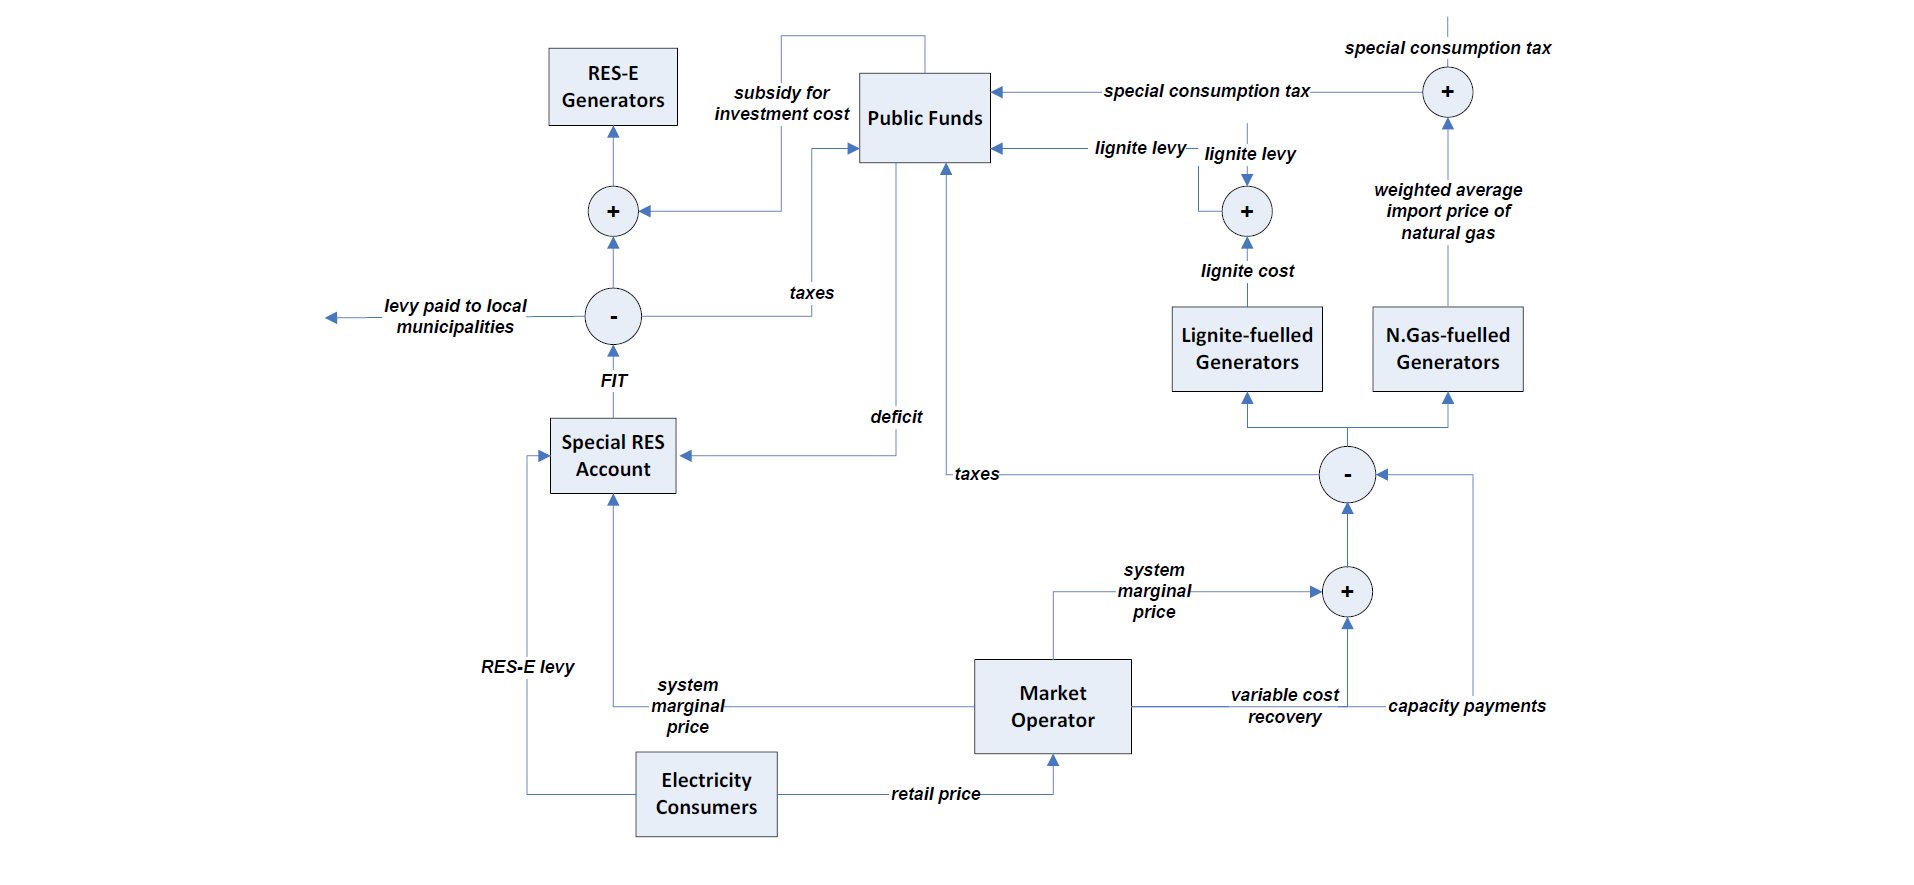
\includegraphics[width=1.4\textwidth]{fig/mon_flows.png}}%
  \caption{���������� ���� ���� �������� ����� ���������� ���������}
  \label{figure:30}
\end{figure}

\section{\tl{Variable Cost Recovery Mechanism} ��� \tl{Capacity Adequacy Mechanism}}

��� ��� 1/5/2008 ���� ����� �� ���� ���� ���������� ��������� ���������� ������� (\tl{Variable Cost Recovery Mechanism}) � ������ ����� �������� �� ������� ��������� ���� �� 10\% ��� ���������� ���� ������� �� ��������� ��� ��� ������� �� �� ��������� ���� ��� ������ ��� ��� ����� ���������. � ���������� ����� ���������� �� ��������� �� �� ������� ��� �� �� ����������� ������� ��������� ������� �� ���������� ��� 30\% ��� ������������� ���� �� ����� ����������� ��� ���������� ���� ������� ������ � ���� ���� ��� ���������� ��� �������� ���� ����� ����� ��� � ���������� ��� ����� ���������� ���� �������.
\newpage
� ���������� ��������� ������ (\tl{Capacity Adequacy Mechanism)} ��������� �� ������� ��������� �� ����������� ����� ��������� �������� ���� ��� ������ �� ������� ����� �� ���� �� ���������� ����� ��� ������ ������ ����. ���� ��������� ������� ��� �� ������� ����� ��� ����������� ���� ������ ��� ����������� �������������� ������ (\tl{Capacity Availability Tickets}), ��� �� ���� ��� ����� ������ ��� ��� ���� �����������. � ��������� ������� ������������ ��� ���� ������ ����� ���� �� ��� ������ ������������ ��� �������. ���� ���� ����������� � ����� ���������� ��� ��������� ������������ ��� ���� ������� �� ���� �� \tl{Demand Equivalent Forced Outage Rate (EFORd)} ��� ��������� ���� ������ ������� ��� ����������� ��������������. �������� ���� ����������� ���� ���� ������������� 1-\tl{EFORd}. ���� ��������� ������ �� ������� ������� �� ��� ����� ���� �� �������� ��� ���� ��� �� ��� ��������� ������������ ��� ������������ ���������������� �� ��� ����� �� ����������� $P^{NCP}$ ��� ��� ���� ��� � ������ ���� ������� ��������� ���� �����. ��� ���������� ��� ����� ��� �������� ��� ������ \tl{j} �����:

\begin{equation}
P^{NCP}\cdot (1-EFORd_j)^2
\end{equation}
\newpage
\section{��� ��� ������� ���������}

������� �� �� ������ ����������� �������, ��� � �������� ��� ��� ������ �� ������������� ��� ������ ���������� ���������. �� ������� ���������� ��������� (��������, ������ �����, �������������) ��������� �� �������� ������. �� ����������, � �������� ��� ��� ������ �� �������� �� �������� ������ ��� ��������� �� ������� ��� �������������� �������. ���� ������ ��� �� ������������ ��� ������������ ��������� ��� ��� ����� �� ���������������� ��� ������ ��� ������� �������, ������� �� ��� ����� �� ���������� ����� ���� �� ��� ������ ��������� (� �������� ����� ��������������), ��� ���������� ��� �� ���������� ��� ��������� ������ ������. � ������ ��� ��������� ����� ���� � ��������� ��������� ��� ������� ��� ������ ��� ��������������� ��� ��� ������������ ��� �������� ����������� (������ ��� ��������� ��� ����������� ���������) ��� ���� ��������� ��� ���� �������� ������� �������. ��� ��������� ����� �� ������ ���� ����������� ���� �� ����� ������������� � ���� ��� ������� �� ��� ������� ���������. ��� ����� \ref{figure:90} ������������� � ������� ��������� ���� �������� ����� ���������� ���������. ���� ��������� �� ��������� ��� � �������� ��� ���������� ��������� ��� ��������� ������ �� ����� ����� ��� �� ��� ��������� �������� ��� ��� �������� ������. ��������, ��� ������ ���� �������� ��� ��� ������ �� �������� �� ������� ������ ��� ��������� ��� �� ����������� ����� ���������.

\begin{figure}
  \makebox[\textwidth][c]{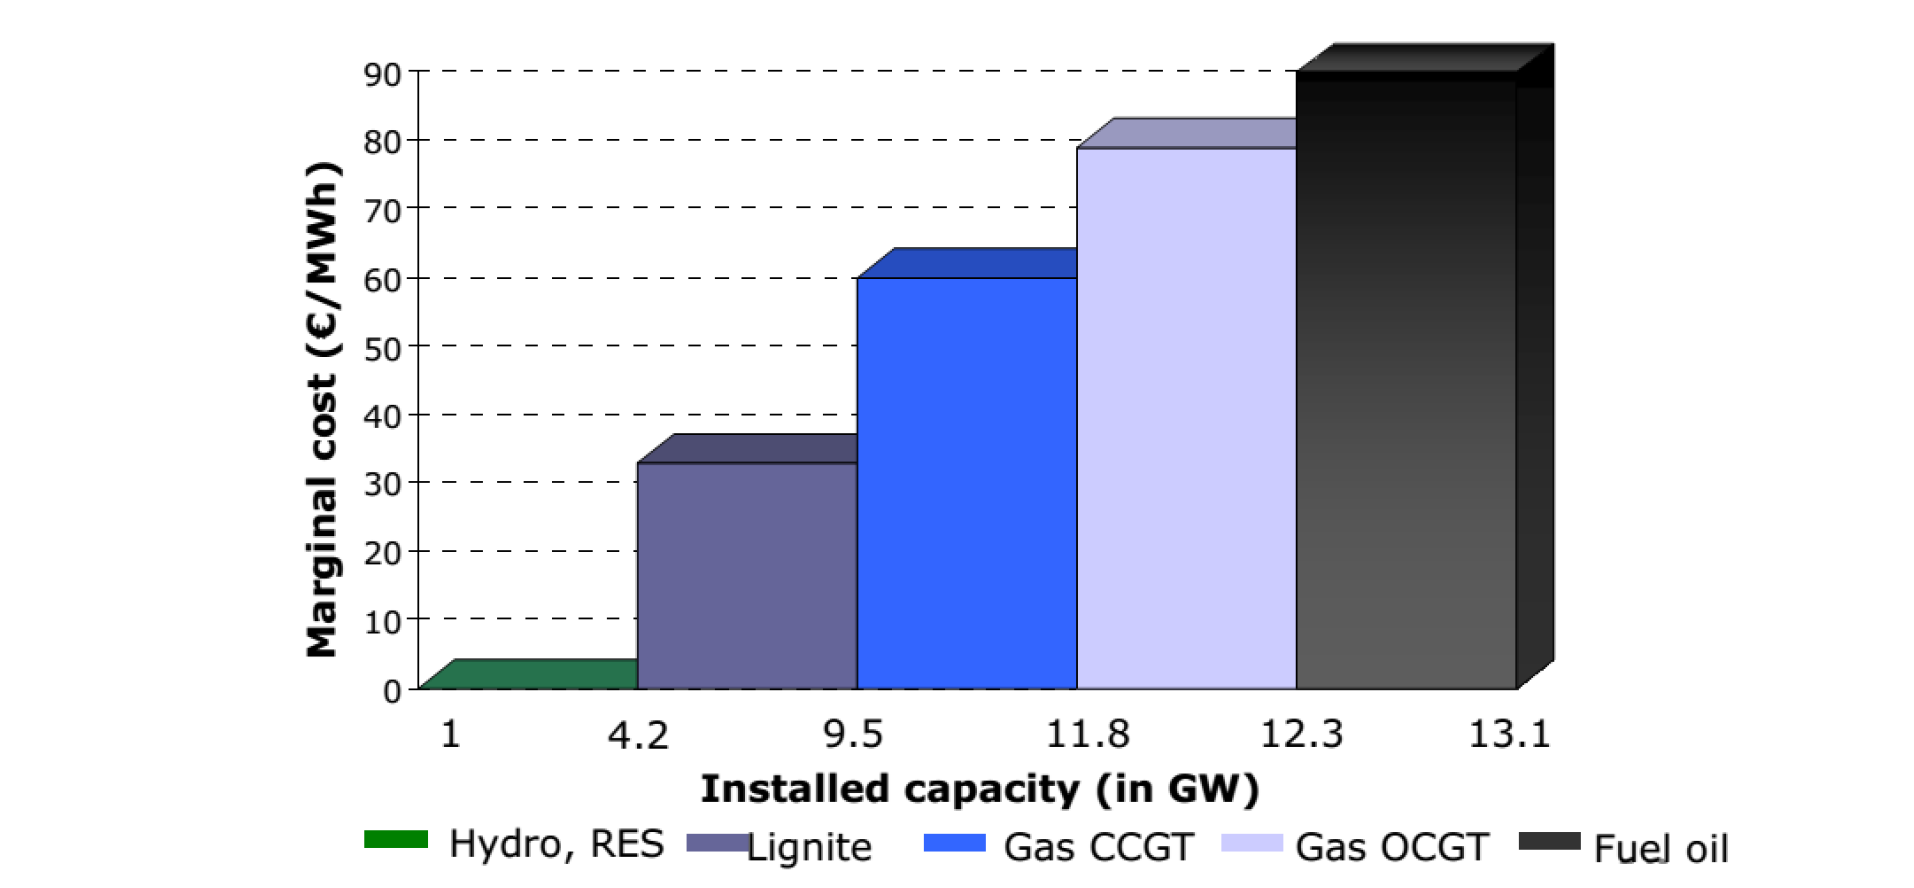
\includegraphics[width=1.3\textwidth]{fig/wholesale.png}}%
  \caption{������� ��������� ��������� ������ ���������� ���������}
  \label{figure:90}
\end{figure}

\section{���������� ��� ������� ��� �����}

�� ������ ��� ���������� ���������� ��� ������� ��� ����� ��� ���������� ��������� ������������:
\begin{itemize}
  \item � ������ ��� ���������� ���������. ��� ��������� ����� �� ������ ���� ����������� ������������� ���� �� ����� � ���� ��� �������� ������� �� ��� ������� ���������. ��� � ���� ������������� ���� �� �����, ���� ������� �� ������ ������ ��� ��� ����������� ��� �������.
  \item � �������� ��� ��� � ����� ��������� �������� ������.
  \item �� ����� ��� �������� �� ������ ���������� �� ��������� ������ ��� ������� ���������. �� ����� ��� ������� ����� ��������� ������� ��� ��� ��� ������� ������ �����: 
\begin{enumerate}
  \item ����� ������ �������� ������������ ��� ��� ����� ��� ������� ������
  \item ���� ����� ���� ���������� ������� �� ���������� ������� ����� ��� �������� ���������.
\end{enumerate} 
  \item � ������������� ��� �����. � �� ������������� ��� ������� ����������� ������� �������, ���� � �������� ��� �� ��������, ���������� ��� ������� ��������� ���� �� ��������, �� ����� ���������� �� �� ��������� ��� �������� �� ������ �������� ��� ��� ������ ��� ������� ���� �� ���� ����. ��� ��� ���� ������ � �� ������������� ��� ����������� ��� ����������� �� ������ ����� ��� ������ ���� ����� �� ������ �����, ������������ ������ ��� ��������� ������������� ��� ������. �� ��������� ���� ������������ �� �� ������ ���������� �� ��� �������� ��������� ������������.
\end{itemize}

\section{������ �����}

�� ��� ����� ���� �� ���� ������ ����� ������� �� ������ �� ������ ��� ������� ����� ������ ��� ����������� ��� ��� ����� ��� ��������. �� \tl{Jong} ��� \tl{Schneider} (2009) ��������� ������ ������� ������ �� ����� �� ��� ����� ���������� ���������� ��������� ��� \tl{Amsterdam}, ��������� ��� �� ������ ����� ���������� ����� ���� ������� ���������. �� ������� ��� ��������� ������� ��� �� ������ ����� ��� �� ����� ���������� ��������� ����� ����� �������������� �� ������������� ������� ����� \citepri{de2009cointegration}. 

�� \tl{Bosco et al.} (2010) ��������� ��� ��������������� ��� �������� ���� ����� ���������� ��������� �� ��� ������� ���������� �����. �� ������������ ��� �������� ���� ������������ ��� �������� �������� ������������� ������ ��� ��������� ������� (������, ��������, ���� �����, �������). � ���� ��� ������� �� ����� ��� �������� ������ ���������� ��������� �������� �� ����� ����� ��� ��� ��� ����� ��� ������� ������ \citepri{bosco2010long}. 
\newpage
�� ���� ������, �� \tl{Ferkingstad et al.} (2010) �������� ��� �� ����� ��� ������� ������ ����� ������ ��������� �� ��� ����� ��� ���������� ��������� ��� � �������� ��� �� ��������� ����� �������� ���������� ���������� ���� ��������� ��� ����� \citepri{ferkingstad2011causal}. 

�� \tl{Furio} ��� \tl{Chulia (2012)} ������������� �� ������� \tl{VECM} ��� �� ������������ ���� ��������� ������� ������ ��� ���������� ��������� ��� ��������, ��� ����� ���������� ��� ��� ������� ������ ��� ���� ���� ��� ������������ �����. �� �������� ���� ������������ ��� �� ���� ��������� ��� �� ������ ����� ����� ���� �������� ���� ���� ���������� ����������� ��� ����� ��� ���������� ��������� ��� ��������� ������ \citepri{furio2012price}.

���� ������� ����������� �� ����� ��� ��������� ��� �� �� ������� ���������� �������� ����� ������ ��� ������� ������ ��� ��� ����� ��� ���������� ���������.

\section{��������� ������� ������ ����������}

����������� �� ������������ �� ������� ��� ���������� ��� ������, ������ ������ �� ����������� ����� �� ����� �� \tl{predictors} ��� �� ��������������� ���� �������. �� ������ ��� ���������� ��� �� ������� �� ������ �� ���� ��� ��������� ���������:

\begin{enumerate}
  \item �� ���������� ����� ��������� ��� ��� ������ ��� ��� ������� ���������� �������� �������� ��� ��� ���������� ��������� �� ���� � ������������� \tl{predictors}. 
  \item ���������������� ���� �� �������� �� �� ������� ����������. ���� ������� ����� �� ������ ���������� ���������� ���� �� ������ ��� �������� �� �������� ���� ���������� ��� ����� ���������� ��� ��� ����������� ��� �� ��������� �� ���������� ��� ����������� ����������, ����� ��� �� ������� ��� �� ���� ���� �������. ���� �� �������� �� ��� ��������� ������ ��� ������������� ��� ��� ��������� ���, �� �� ������, �� ����� ������������. 
  \item �� ���������� �����, �� �������� �������������� ���������� ��� ���������� ������ ��� ������� ������������. ��������, � ����������� ��������� ������������� ���������� ��� ������� �� ����� ���� ��������� ����������� ��� ���� ���������� �� ������������� �� ���������� �����.
\end{enumerate}

\begin{figure}
  \makebox[\textwidth][c]{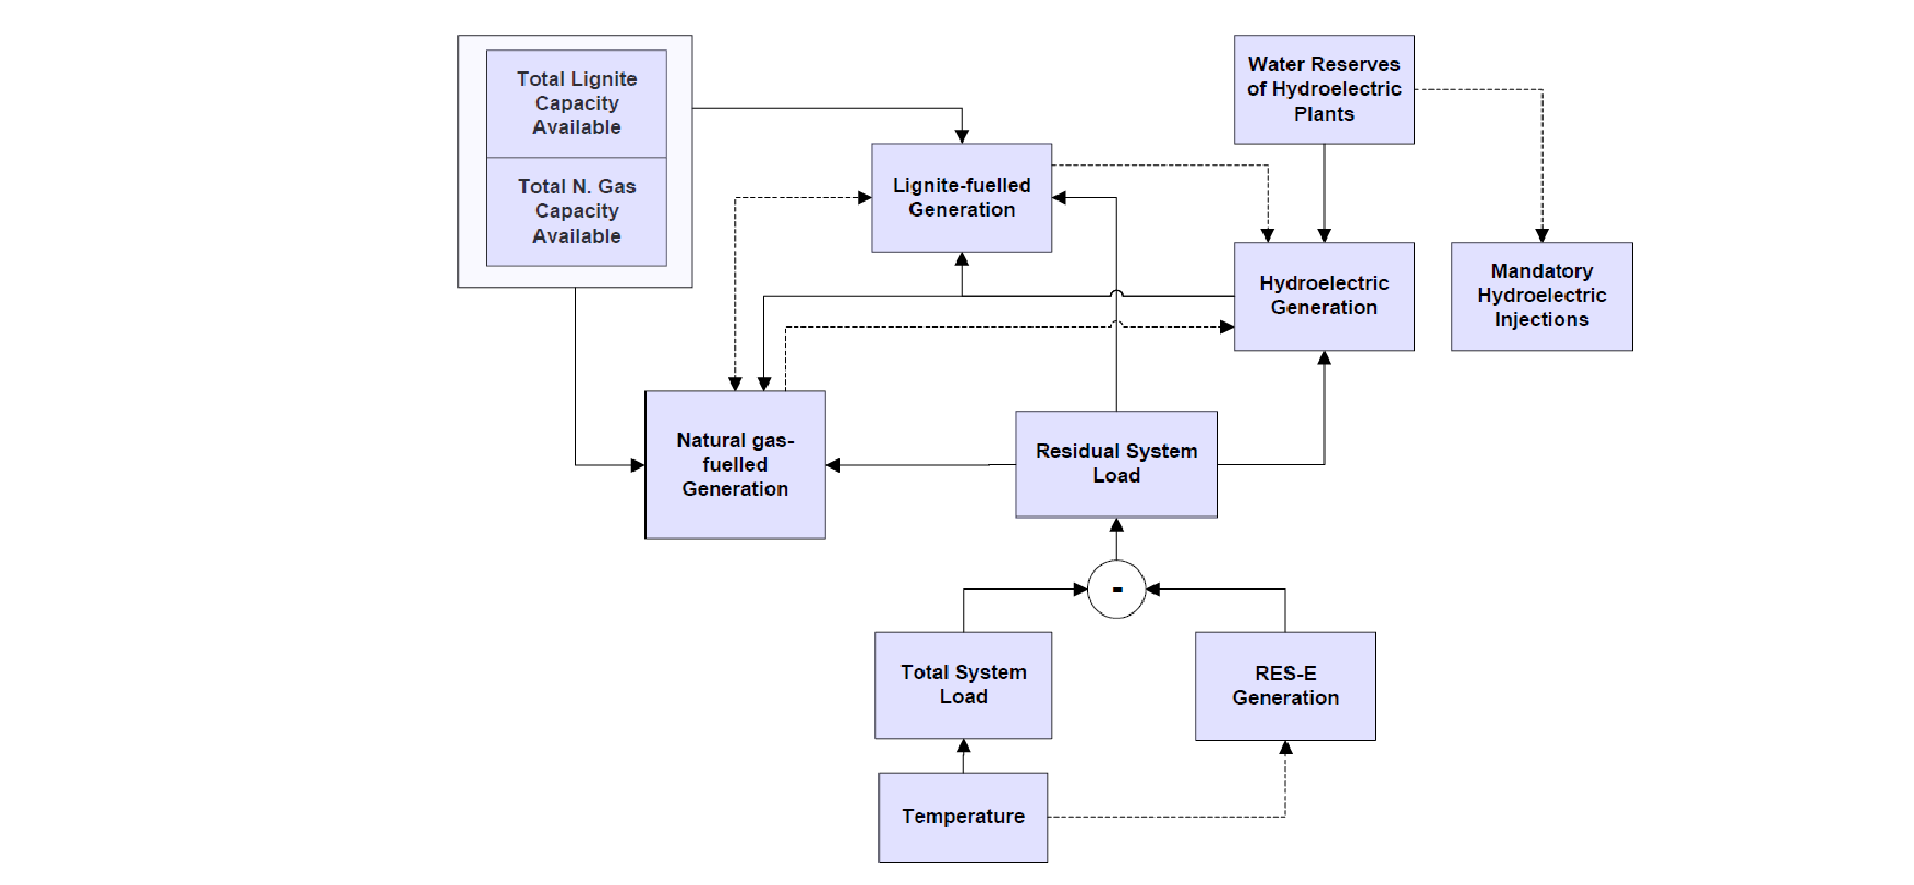
\includegraphics[width=1.3\textwidth]{fig/causal_relationships.png}}%
  \caption{��������� ������� ���� �������� ����� ���������� ���������}
  \label{figure:91}
\end{figure}

�� ��������� ������� ��� ��� �������� ����� ���������� ��������� �������������� ��� ����� \ref{figure:91}. �� ������� ���� ��������������� ������� �� ������ ������� ��������, ��� �� ������������ ������� ��� ����� ������ ��� ��������, ���� ������������ ������ ��� ����.
\newpage

� ���� �������� �������� ��������������� ��� �� ������ ���: \\

\textit{�� �� ������ $z_t$ �������� ��� ����� ��� ���������� ����������� �������������� ���������� �������� �� ������� ��� �������� �� ���� ��� \tl{lagged} ���������� ��� ������ $Y_t$ ���� ��� ��� $Z_t$. �� � �������� ���� ������ �� ��������� ���� ��� \tl{lagged values} ��� ���������� $W_t$ (� ����� �������� ����������� ��� ��� ����� $Y_{t+1}$ ������� ��� �������� ����� (\tl{Granger causal flow}) ������ ��� $W_t$ ��� $Y_t$ ($W_t \to Y_t$).} \\

�� ������ �� ���������� ��� � ��� \tl{Granger} ������ ��� ��������� ��� ����������, ��� ��������� ��� ���, ��� ��������� ������� ��� ��� ��������� ���������� �������������, ���� ��� ������ ���������� ���� �� ���������� ������� �� ��������� �� ���������. ������ �� ����� �� �� ������, �� ����������� ��� ��������������� ����� ���� ����� ���������, ��������� ��� ��������� ��������� �������� �� �������� ����� ��� �������� ���� ���� ��� ����� ������. ���� ��������, ��� ��� ��������� ���� �� ����������� �������������� ��� ������� ���� ��� ��� ��������� ��������, �� ������� ��� ������ ���������� ��� ��������� ��������, �� ������ ��� ������������� ��� ���� ��������� � ���������� ��� ��� ����������, ���� � �������� ��������� ���������� ��������� ��� ���� ��������. ��� ��� ���� ������, � �������� ����� ������ ��� ������� ������ ��� ��� �������� �������, ����� ��� ������ ����� ��� ��� �������������� ���������, �� ������ �� ��������� ��������������.

\newpage
\thispagestyle{empty}

\chapter{�������������� ���������}

\section{��������}

���� ��� ������� ���������������� �������� ��� ��� ����� ���������� ���������, ���� �� �������� �� ������ �������. �� �������� ���� �� ����� \tl{comma-separated values}(\tl{csv}). �������� � ������� ��� �� ���������� ��� ���������������� ������ ���� ������ \tl{python}. �� \tl{SMP} ����� � ������ \tl{y} ��� ������� �� ����������� �� ���� �� �������������� \tl{X} ��� �� ������ �� ������. 
\newline
��� ������������ ��� �� ������������ �������������� \tl{snippets} ��� ������ ��� ��� ��������� � ������� ���� �� ������ ���������� ������ �� ������� ��� �� ��� ����� � ����������. � ������ ����� ���� ������ ��������������� \tl{python} �� ����� ����������������� ����������� ��� \tl{machine learning} �� ������ ���������������� ��� ��������� ���� ��� ������� �������� ��� ����� (\citealpsec{sklearn}).

\subsection{\tl{SMP}} ���� ��� ���������� ��������� ��� ������������� ����� ��� �������� ��� 1/1/2008 ��� 30/9/2013. � ����� ����� �������� ����������� ��� �� ��������� 24 ������ ��������� ��� ���� ��� ���������� ��������� ��� ���� ��� ��� ������. �� ��������� ��� ��� ��� �� �������������� ��� �� ���������� ���� ������� ������� ��������� ����� ��� �������� ��� 1/1/2009 ��� 30/9/2013 �������� �� \tl{SMP} �� ���� ������������ ������� ��� ��� ��� ������ ������. 

\begin{minted}[linenos]{python}
import pandas as pd
import datetime
path = "C:/Users/Dimitris/Desktop/diploma/data/"
df = pd.read_csv(path + "smp.csv", sep=',', converters={0:str2date})
df = df.set_index('Unnamed: 0')
runfile('C:/Users/Dimitris/Desktop/diploma/data/data2.py')
df.describe()
\end{minted}

\begin{figure}
  \makebox[\textwidth][c]{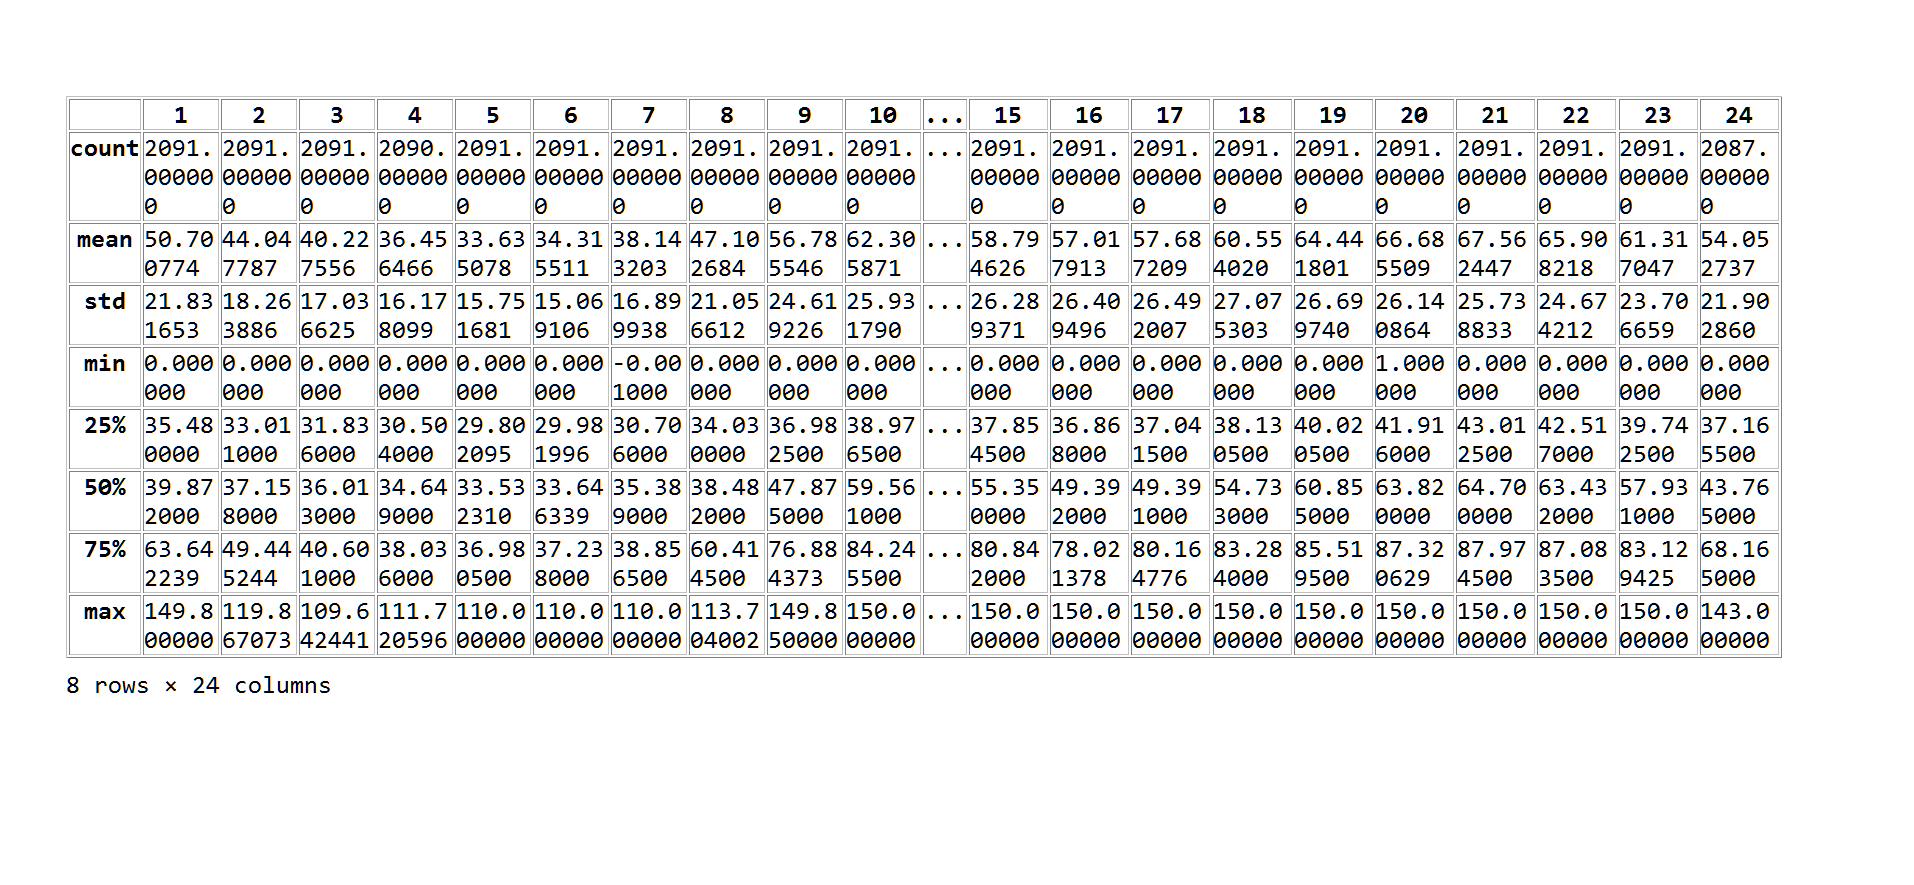
\includegraphics[width=1.4\textwidth]{fig/smp_describe.png}}%
  \caption{\tl{SMP}}
  \label{figure:10}
\end{figure}

\newpage

������ 24 ������ ��������� ��� 2091 �������. ���� �� ������ ��������� \tl{floating point} �������� �� ����������. ����������� ��� � ���� ���� ��� \tl{SMP} ���������� ����� ��� 50\euro �������������� ������� ������������ ���� ���� �����. ��� ������ ���� ����� ��������� ����� ��� 40\euro ��� ������� ��� ��������. � ������ �������� ����� ��� 25\euro �� �������� ����� �� ��� ��������� �� 150\euro. �� ��������� ����� ��� \tl{SMP} ����� ���������, ��� ���� ��������� ��� ������� ��� ������ \tl{missing values} ��� ������ ��� �� ����� �� ������������ ���� ��� ��������������. ���� ��� ������� �� ������ ��� ����� ��������� ����� ��� \tl{SMP} ���� �� �������� �� ��������� ������������. 

\subsection{��������������}

�� �������������� �� ���� �� ����� �� ����� � ������� ��� �������������� ��������. ����������� ��� ���� ������� ��� ���������� �� �������� �������� ������ ��� ��� �� ������.
\newline

\begin{description}
  \item[\tl{availability}] ������������ ������� ��������� ������� ���� ���� �� \tl{MW}.
  \item[\tl{exports}] �������� ������ ������� ���������� ��������� �� \tl{MW} ��� ��� ������ ���� ���� �������� ���.
  \item[\tl{hydrogen}] �������� ������ �������� �������������� ����������� �� \tl{MW}.
  \item[\tl{imports}]  �������� ������ �������� ���������� ��������� �� \tl{MW} ��� �������.
  \item[\tl{lignite}]  �������� ������ �������� ������� �� \tl{MW}.
  \item[\tl{load\_forecast}] �������� ������ ������.
  \item[\tl{ngas}] �������� ������ �������� ������� ������ �� \tl{MW}.
  \item[\tl{res\_forecast}] ������ �������� ��������� ��� ����������� ����� ��������� �� \tl{MW} (�������� ������).
  \item[\tl{waters}] �������� ������ �������� ��� �� ����������� ���� �� \tl{MW}.
  \item[\tl{waip}] ������� ���� ������� ������.
\end{description}

\section{��������������}

\subsection{���������� ������� ������� ���������}

������ �� �������������� ��� .\tl{csv} ������ �� ����� �� �������� ��� ��������� ��������� ����� ��� ��������������� ���� ��� ��� \tl{SMP}. ��� �� �� ��������� ���� ����� �� ������� �� �������� ��� ����� ���� ������ ��� ������� ��� �� �������������� ��� ��� ����� ��� �� �������� �� ���������� ��������������. ������ ���� ��� ����� ��� ������������ �� ��� ��� ������ �� ����� �� ����� �� ������ �� �� ����� �� ����� � �������. ���� ��������� ��� \tl{SMP} ������������ ��� ���� ��� ��� ��������������� ���� ������ ��� ���� ��������� ��� \tl{waip} �� ������ ��� ���� ���� �� �������� ��� ����. � ��������� ����� ���� ������. ���� ��� ���������� ��� ������������ ��� ��� ������ \tl{out.csv} �� ����� �� �������� ��� ��� ����� ��� ��� ���� \tl{X} ��� ���� ��� ������ ��� ������ ��� ������ ������, ��� ����� \tl{a} ��� ��� ����� \tl{b}. ����:

\begin{minted}[linenos]{python}
df ['X'] = df['a'] + df['b']
out['X'] = df['X']
\end{minted}

������������ �� �������� ����� �� ������ ������ �� ����� ���� ����� ����� �������� ��� ����� ��� \tl{SMP} ��� ���� �������� �� �������������� ����� ����������� �� ������ �� ������� �� �������� \tl{SMP} �� \tl{p}-�������� ���� �� ���� �������� ����� ��� ���� ������ 1/1/2008 ��� 30/9/2013 (������ 1795 ��������) ��� ������ ��� ������ \tl{Y} �� \tl{NxP} �������� ���� N � ������� ��� ���������������, ������ 10. ���������� �� ������ ��� ��������� �� �������������� ��� ��������� ��� ����� \ref{figure:11}.

\begin{figure}
  \makebox[\textwidth][c]{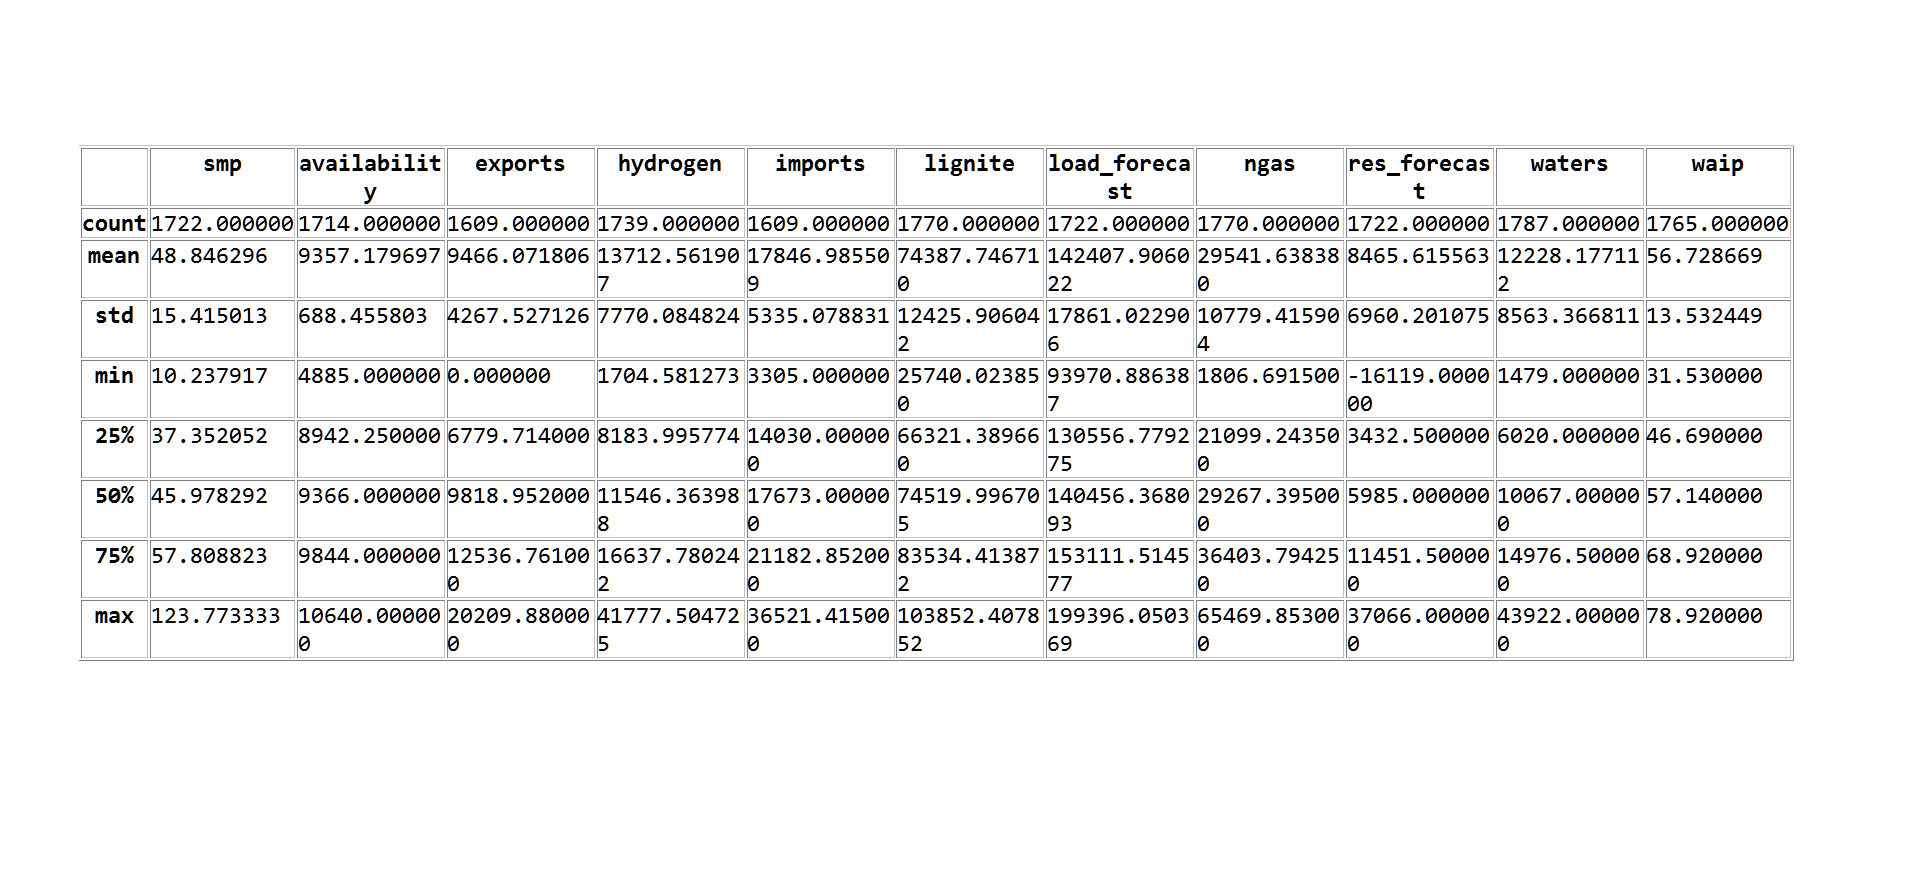
\includegraphics[width=1.4\textwidth]{fig/teliko_describe.png}}%
  \caption{�������������� ���������� ����������}
  \label{figure:11}
\end{figure}

�� \tl{SMP} ����������� ��� ����������� ��� ���������� ���� ����������� ���������. ����������� ��� ���� �� ���������� ����� ����� ��� �������. � �������� ������������ ��� ��� ������ �� ������� ���� ���� ���� ����� ������ ��������, �� ����� �������� ��� � ������������ ��� ����������� ��������� ������ ������� ��� �������� ��� ���� ��� ��������.
\newpage

\subsection{��������� \tl{missing values}}

��� �� ������� �� ���������� ��� ����������� ��� ����� ����� ��� �������� �� ���������, ������ �� ��� ������ ����� ��� �� ������� ��� �� �������� ���. �������� �������� ������ ��������� ���������� ��� ������� \citepri{saar2007handling}.
\begin{enumerate}
  \item �������� ��� ��������� ��� �������. ����� ��� ���������� ��� ��������������� ����� ��� ���� ���������, ��������� �� �� �������� ��� ������� ����� ������ ������������. ���� �����, � �������� ����� ��������� ���� ����� ������ �� ��������� �� ������� ��� �������� �� ������������ \tl{instances} ��� ��������� ���. ���� ��������� ��� ����������� ���������� ��� ��� �� \tl{instances} ��� ��������� ���.
  \item �������� ��� ��������� ��� �������. �������� ����������� ��� � �������� ��� ��������� ����� ������.
  \item \tl �������� ��� ����� ��� ������ (\tl{imputation}). ���� ��� ���� ��� ������ �������������� ��� ��� ���� ���� � �������� ��� ������� ����� ��� ������� ��������� ��� ������������� ��� ������� ��� ��������� ���������� ������������. �������� ������� ������� ��� \tl{imputation}.
  \begin{enumerate}
    \item \tl{(Predictive) Value Imputation (PVI)}: �� \tl{missing values} �������������� ��� ����������� ����� ���� ��� ������� ��� �������. �� ������� ����������� ����� � ����� ����, � �������� � � ��� ����� ����.
    \item \tl{Distribution based Imputation (DBI)} ��������� ���� �������� ���� ��� ��� ����, ������� �� ������ �������� ���������� ���� ��� ��� ���� ���� ��� � ���� �������� �� ���� ��� �����, ��� �� ���������� �� ����� � ���������� ��� ���������� �����. ���������� ����� � ���������� \tl{C}4.5.
    \item \tl{Unique value imputation}: ���� �� ������� ������������� ���� ��� ���������� �� ��� ���� ����, �������� ������� ��� ������������� �������� ��� ����� ��� ������ �� ���������. ���� �� ������� ���������� �������� ���� � ��������� ��� ������ ��������� ����������� ��� ��� ���� ��� ���������� ��� ������ ��� ������ � ����.
	\end{enumerate}
\end{enumerate}

� ���������� \tl{sklearn} ���� ��������� ����������� ��� \tl{machine learning} ��� ����� � ����� ���������� ��� ��������������� ���� ������� ���. ���� ������ ����������� ��� \tl{preprocessing} ���������. � ����� \tl{Imputer} ����� predictive value imputation ��� missing values, ������� �� ������ ��������. �� \tl{default} �������� ����� � ����� ���� ��� �����, ������ ��� ��������������� ���. �������� �� ��� ��������� ������� ������� ����� ��� \tl{missing values} ��� ���������� �� �������� �� ����� ������ ���� �� ������� �� ���������� ��� ����������� ��� �� ���������������.

\begin{minted}[linenos]{python}
from sklearn.preprocessing import Imputer
imp = Imputer(missing_values='NaN', strategy='mean', axis=0,verbose=0)
imp.fit(df)
train_imp = imp.transform(df)
\end{minted}

\subsection{\tl{Train and Validation Sets}}

������� ���� ����� �� ��������� �� �������� ��� ������ �� ��� ���: ������� (\tl{training}) ��� ���������� (\tl{validation}). ��� ����� �� ���������� �� ������ �� �������� ��� ��� ���������� ����� ��� �� ������������� \tl{patterns} ��� ���������� �� ����� �� ������ ���������, ��� ��� ������� �� ������ ���������� �� ���� �� ������� ��� �� ����� ������������. �� �������� ������� ������ �� ��� ������� ��� ���������� \tl{train\_test\_split} ��� \tl{sklearn}.

\begin{minted}[linenos]{python}
from sklearn.cross_validation import train_test_split as ts
dataset = train_imp[:,1:]
smp = train_imp[:,0]
dataset_train, dataset_test,smp_train, smp_test= ts(dataset,smp, test_size=0.33)
\end{minted}

��� �������� ���������� ������ ������������ ��� �������, ���� � ������ �������� ���� �� \tl{SMP} ��� � �������� �� �������������� ��� ������ ������������ ��� ��� ��� �� ������. �� ��� ��������� \tl{random state} �������� �� �������������� ������ ��� �� ��������� ��� ���������� ���� �� ������ �����, ���� ��� ����� ���� �������. ������ �� ������ ��� ������� ����� 67\% ��� �� ���������� ��� ��������� 33\% ���� �� ��������� �������� \tl{fit} ��� ��������.
 
\newpage
\thispagestyle{empty}
\chapter{������� ��������� ��� ����������}

\section{��������}

��� �������� ���� �� ����������� ��� ����������� ��� ���������� �� �������� ��� ���������� �� ������ \tl{training} ��� \tl{test sets}. ���� ������� ���� �� ������������ ��� ���������� ��� ���������� ��� ��� ������������ ���� ��������� ���� ��������� ��������. ���� ��� ������� \tl{training} ��� \tl{validation sets}, � ���������� ��� ������������� ����� �����, ��� ������ �� �������� ���� ����������. �� ���� ��� ����� ����������� �������� ���� ��� ��� �� ����������� ��������, ���� ��� ���� ������ �������� �� ����������� ��� �������������� ��� ���������� �� �������� �� ������. �������� ���� �� ����� ��� ��������� �� ���������� �� ��� ���� ���� ����� ��� ����������� ��� ���� �������� ���� ��� �� ���� ��������� ����� � ���� ��������� ���� ��������� ��� ������. 

\section{\tl{Multicollinearity}}

�� ���� �� ������ ��������� �� ���������� ��� �� �������������� ��� ���������� ��� ������� �� ������������ ������ ��� �������������� ��� ���� ��������� �� ������������ ��� ���������� ������, ���� ��������� ��� ����� ���� ��� ������� �������� ���� ������ ��� ���� ���������� ���������. ������ �� ���������� ������ �� ������������ ����� ������������� ���� ��� \tl{multicollinearity}, ������ �� ������������ ��� ������� ���� ��������� (���� ��� ������ ��� ��������� ����) � ����� ��� ��� ����� ���������� ��� ����� ���������. ���� ������������ \tl{collinearity} ������ ��� \tl{predictors} ������ �� ������ ���� ������� ��� ����� ������ ����, ��� �� ���� � ����� ����� ��������, ������ ��� ������: $X_{2i} = \lambda_0 + \lambda_1X_{1i}$ ���� ���� ��� �� ���������� ����� \tl{perfectly collinear}. �� ���� ������ ��������� ��������� �������� ��� ������ ������������ ����������, ���� ������ \tl{multicollinearity}. ������ \tl{perfect multicollinearity} �� � �������� ����� ��������, ������ ��� ������:
\begin{equation}
\lambda_0 + \lambda_1X_{1i}+\lambda_2X_{2i}+\dots +\lambda_kX_{ki} = 0
\end{equation}

��� �� ������ ��� �������� ������ ��� �������������� ��� ���� \tl{predictor} �� �������������� ������ \tl{bar charts}. ���� ���� ������� ���� �� ������������ �� ������� ��� ��� ������ ��� ���������� �� ����. ���� ��� ������� ��� ����������� ��� �������� 8 �� ������� \tl{partial dependence plots} �� ����� ����� ��� ������ ��� �������� ��� ���������� ����� ��� ������ ���� ���������� �� �� ������ ��� ����������. 

\section{��������}
��� ������� ������ \tl{regression} ����� � ������ ��� ������� ����� �������� �������� �� ���������������� ��� ����������� �����������. �� ������ ��� ������������� ��� ����� ���� ����������� �����:
\begin{enumerate}
\item ���������� ��� ��������. ���� ������������ ��������� �� ���������������� �������� ��� ����������� ��� \tl{scikit-learn}
\item �������� ��� �������� ��� \tl{training set}
\item ���������� ��� \tl{validation set}
\item ������� �������������
\end{enumerate}

��� ��� ������� ��������� �� ���������������� �� �������� ��������.

\begin{equation}
explained\_variance(y,\widehat{y}) = 1 - \frac{Var\left \{ y -\widehat{y}\right \}}{Var\left \{ y \right \}}
\end{equation}

\begin{equation}
MAE(y,\widehat{y}) = \frac{1}{n_{samples}}\sum_{i=0}^{n_{samples}-1}|y_i-\widehat{y_i}| 
\end{equation}

\begin{equation}
MSE(y,\widehat{y}) = \frac{1}{n_{samples}}\sum_{i=0}^{n_{samples}-1}(y_i-\widehat{y_i})^2
\end{equation}

\begin{equation}
R^2(y,\overline{y}) = 1 - \frac{\sum_{i=0}^{n_{samples}-1}(y_i-\widehat{y_i})^2}{\sum_{i=0}^{n_{samples}-1}(y_i-\overline{y_i})^2}
,
\overline{y} = \frac{1}{n_{samples}}\sum_{i=0}^{n_{samples}-1}y_i
\end{equation}
\newpage
\section{\tl{Random Forests}}

\subsection{�������� ���������}

� ������� �� ��������� ��� ��� ��������� \tl{Random Forests}.

\begin{minted}[linenos]{python}
from sklearn.ensemble import RandomForestRegressor
rf = RandomForestRegressor(n_estimators=1000,oob_score=True)
rf.fit(dataset_train, smp_train)
rf.get_params()
y1 = rf.predict(dataset_test)
\end{minted}

�� ������ \tl{RandomForestRegressor} ���� ������������� ������� �������� �� ������ ��� �������� ��� �������� ��� ���������� ��� ���� ������ ��� �������� ��� �� \tl{oob error}. 

\begin{minted}[linenos]{python}
print("Mean accuracy,training set = %f"%(rf.score(dataset_train, smp_train)))
print("Mean accuracy,validation set = %f"%(rf.score(dataset_test, smp_test)))
print 'OOB score: %.2f\n' % rf.oob_score_
\end{minted}

�� ����� ����������: \\
\tl{Mean accuracy,training set = 0.966240 \\
Mean accuracy,validation set = 0.739425 \\
OOB score: 0.75
}

����������� ��� � ���������� ���� ��� ���� ���� ����, �� ����� ������� ��� �������� ������ �� �������� ����� ��� ����� ���, ������ ���� ��������� ��� �� \tl{SMP} �� ���� �� �������������� ��� ��� �������. ���� �������� ��� �� \tl{mean accuracy,validation set} ���� ��� ��� �� \tl{oob score}, �� ����� ��� ���� ��� �������� �� �������� ����� ��� 75\% �� ���������� ����� ��� �����. � ���������� �������� ��� ��� ��������� ����� ���� ���������, ����� ��� 97\%.

������������ ����� ��� ���������. \\

\begin{minted}[linenos]{python}
from sklearn import metrics as skm
print("Explained variance = %f" %(skm.explained_variance_score(smp_test, y1)))
print("Mean absolute error = %f" %(skm.mean_absolute_error(smp_test, y1)))
print("Mean squared error = %f" %(skm.mean_squared_error(smp_test, y1)))
print("R2_score = %f" %(skm.r2_score(smp_test, y1))) 
\end{minted} 

������: \\
\tl{Explained variance = 0.739508 \\
Mean absolute error = 5.456595 \\
Mean squared error = 58.660423 \\
R2\_score = 0.739425}
\newpage
������ �������� �������������� ��� \tl{explained variance} ��� \tl{$R^2$ score} ��� �� \tl{mean absolute error} ��� ������� ���� ����� ����� �� ����� ��� ������������ ���� �����������. �� ���� ������ ����� ���� ���� 5.5 ������� ��� ��� ���������� ����, �� ����� �������� ��� �� ������� ������ �� ��������� �� ���� ���� ������� ��� ������ ����. �� \tl{mean squared error} ����� ��� ���� ��� ��� ���������� ��� ��������� ��� ���������� �� '������ ��������' ��� ���������.

\subsection{\tl{Cross Validation}}
� ������� ��� \tl{cross validation} ����� ��������� ����� ������� ����� � �������� ��� \tl{overfitting} ��� ��������� ���, ����� ��� �� ����������� \tl{training} ��� \tl{test sets}, ����� ������ �� ���������� ��� �������� �� ���������� �� ����� ������ ���� � ��������� �� ���������� �������� ��� ��� ���� �������������� �� ������ ��� ��������. � ����� ��� �� ���� ������ �� ���������� ��� ������� ��� ������ �� ������������ ��� ��������� �� ��� ����� �� ����������. � ���� ������� �� �� �� ���������� ��� ���� ������ ��� �������� ��� �� ������ ����������, �� �������� �� ������������ ��� ������� ����������� ���� ��� ������ �� �������� �� ������� ��� \tl{test set}. ��� ���������� �� �� 5-\tl{fold cross validation} ������������ 5 ������ ��������� ��� ��� �����������, �������� ��� ��������� �� 4 ��� ���� ��� �� ������������ ��� ���������, ��� ���� ������� 5 �����. 

\begin{minted}[linenos]{python}
from sklearn import cross_validation
scores = cross_validation.cross_val_score(rf, dataset_train, smp_train, cv=5)
print 'Cross Validation Scores:' 
print scores 
print "Cross Validation Accuracy: %.2f (+/- %.2f)" % (scores.mean(), scores.std() / 2)
\end{minted}

������ ��� 5-\tl{fold Cross Validation}: \\
\tl{Cross Validation Scores}: \\
$\left [  0.75343825 \; \; \;  0.70602166 \; \; \; 0.76413408 \; \; \; 0.74446292 \; \; \; 0.72598341
\right ]$ \\
\tl{Cross Validation Accuracy}: 0.74 (+/- 0.01) \\

������ ��� 10-\tl{fold Cross Validation}: \\
\tl{Cross Validation Scores}: \\
$\left [  0.786871 \; \; \;    0.66804677 \; \; \;  0.68724677 \; \; \;  0.76931317  \; \; \; 0.7993393 \; \; \;   0.78431832 \right.$ \\
 $ \left. 0.71387939 \; \; \;  0.76512308\; \; \;   0.75068604 \; \; \;  0.68754537
\right ]$ \\
\tl{Cross Validation Accuracy}: 0.74 (+/- 0.02) \\

����������� ��� � ������� ��� ���������� ����� �������� �� ��� ������� ��� ������ ��� \tl{test set} �� ����� �������� ��� �� ������� ��� ����� ������� ��� �� ������ �� ������������ �� �������� ����� ��� �� ������� �� ���� ���� ������������ �� ����������� �������� �� ��� ��������.
\newpage

��� �� ����� ��� ������� ��� ���������� ������� �� �� ����� ��� ���������� �� ���� �� ������ ���, ������� 20 \tl{iterations} ��� ���� 1 ��� 20 (����� 1 �������� ��� �� ������ ���� ���� ��� ����� �� ����� �������������� ��� �������� ���� ��������������� �� ������ ������). �� ������������ ��������� ��� ������� \ref{figure:13} ��� \ref{figure:15}.
\begin{figure}
  \makebox[\textwidth][c]{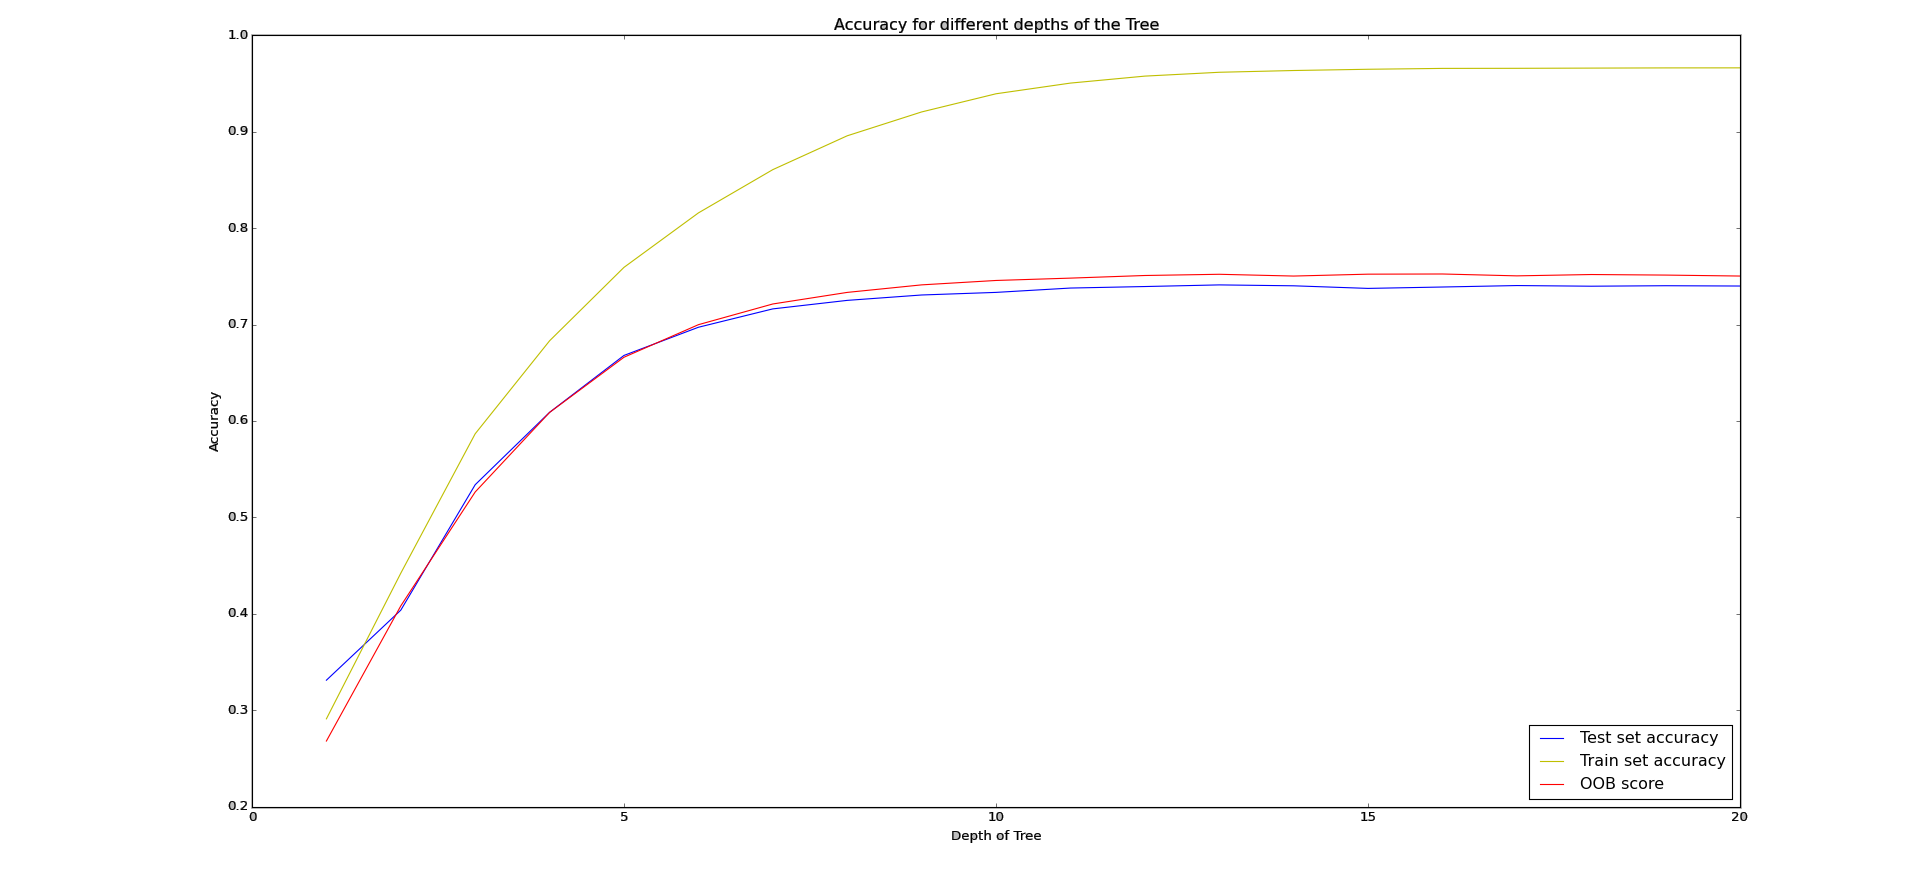
\includegraphics[width=1.4\textwidth]{fig/rf_accuracy_depth.png}}%
  \caption{\tl{Random Forest: Accuracy}}
  \label{figure:13}
\end{figure}

\begin{figure}
  \makebox[\textwidth][c]{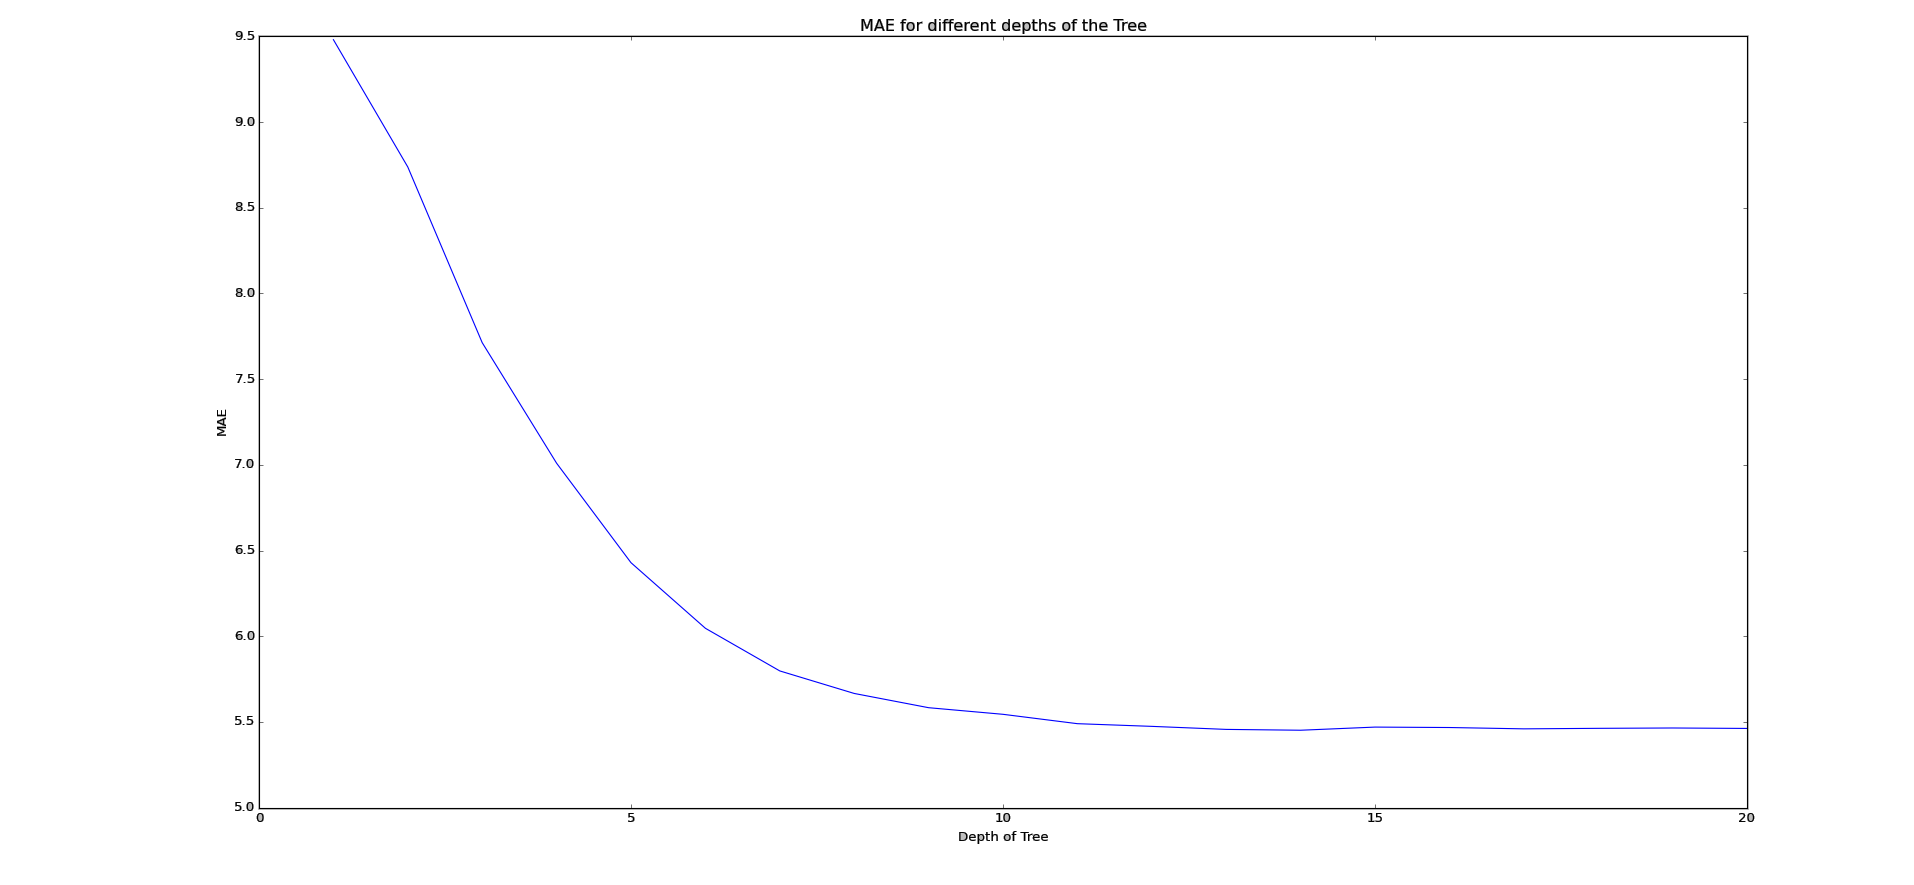
\includegraphics[width=1.4\textwidth]{fig/rf_mae.png}}%
  \caption{\tl{Random Forest: Mean absolute error}}
  \label{figure:14}
\end{figure}

\begin{figure}
  \makebox[\textwidth][c]{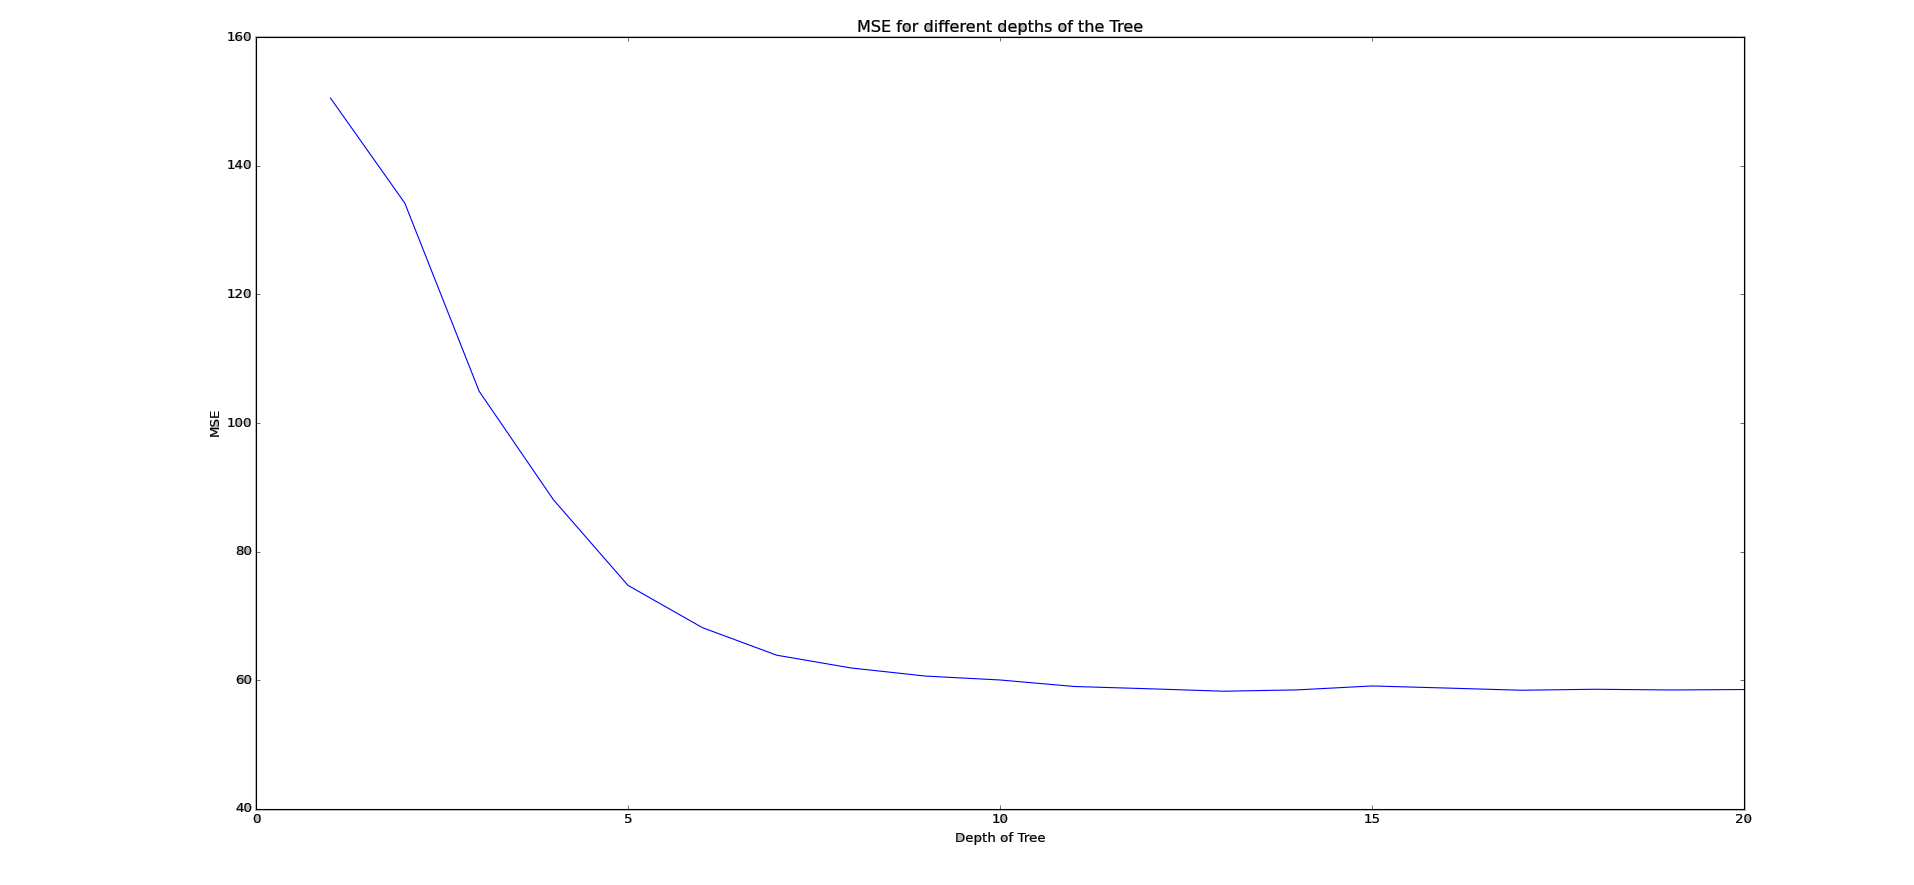
\includegraphics[width=1.4\textwidth]{fig/rf_mse.png}}%
  \caption{\tl{Random Forest: Mean squared error}}
  \label{figure:15}
\end{figure}

��� ����� ���� �������� ��� ������ ������ ��� ���������, ��� 30\% ��� ����� 1 �� 70\% ��� ����� 6. ��� ��� ��� ���� � �������� ��� �������� ������� ��� ����, ��� ���� ��� ����� 12-13 ��� ������� ����� ������, ������ ������� �� ����������� ��� ���� ����� ������. ���� ��������� ��� ������� ��� ���� ��� ��� ������ ������ \tl{overfitting} ��� ��������� ��� ��� �������� �� ����� ��������.

�� ��� ���� ����� �� \tl{MAE} ���� ��� �� \tl{MSE} �������� ���� ������� ��� ��������� �� �����, ���� ���� ��� ��� ������ ������ ����� ��������������� ��� ������� ��� ��� �������� �� ��������� ���� ��������.
\newpage
\subsection{����������� - ������������ ����� \tl{SMP}}

�� ����� \ref{figure:12} ����������� ��� ������� ��� ����������� ����� �� ����� �� ��� ����� ��� ������������ ��� �� \tl{SMP}. � ������ \tl{x} ����������� �� �������� ��� ��� ��� �����, ����� ����� ������ ������� ��� ��������� ���� ��� ��������� ��� �������.

\begin{figure}
  \makebox[\textwidth][c]{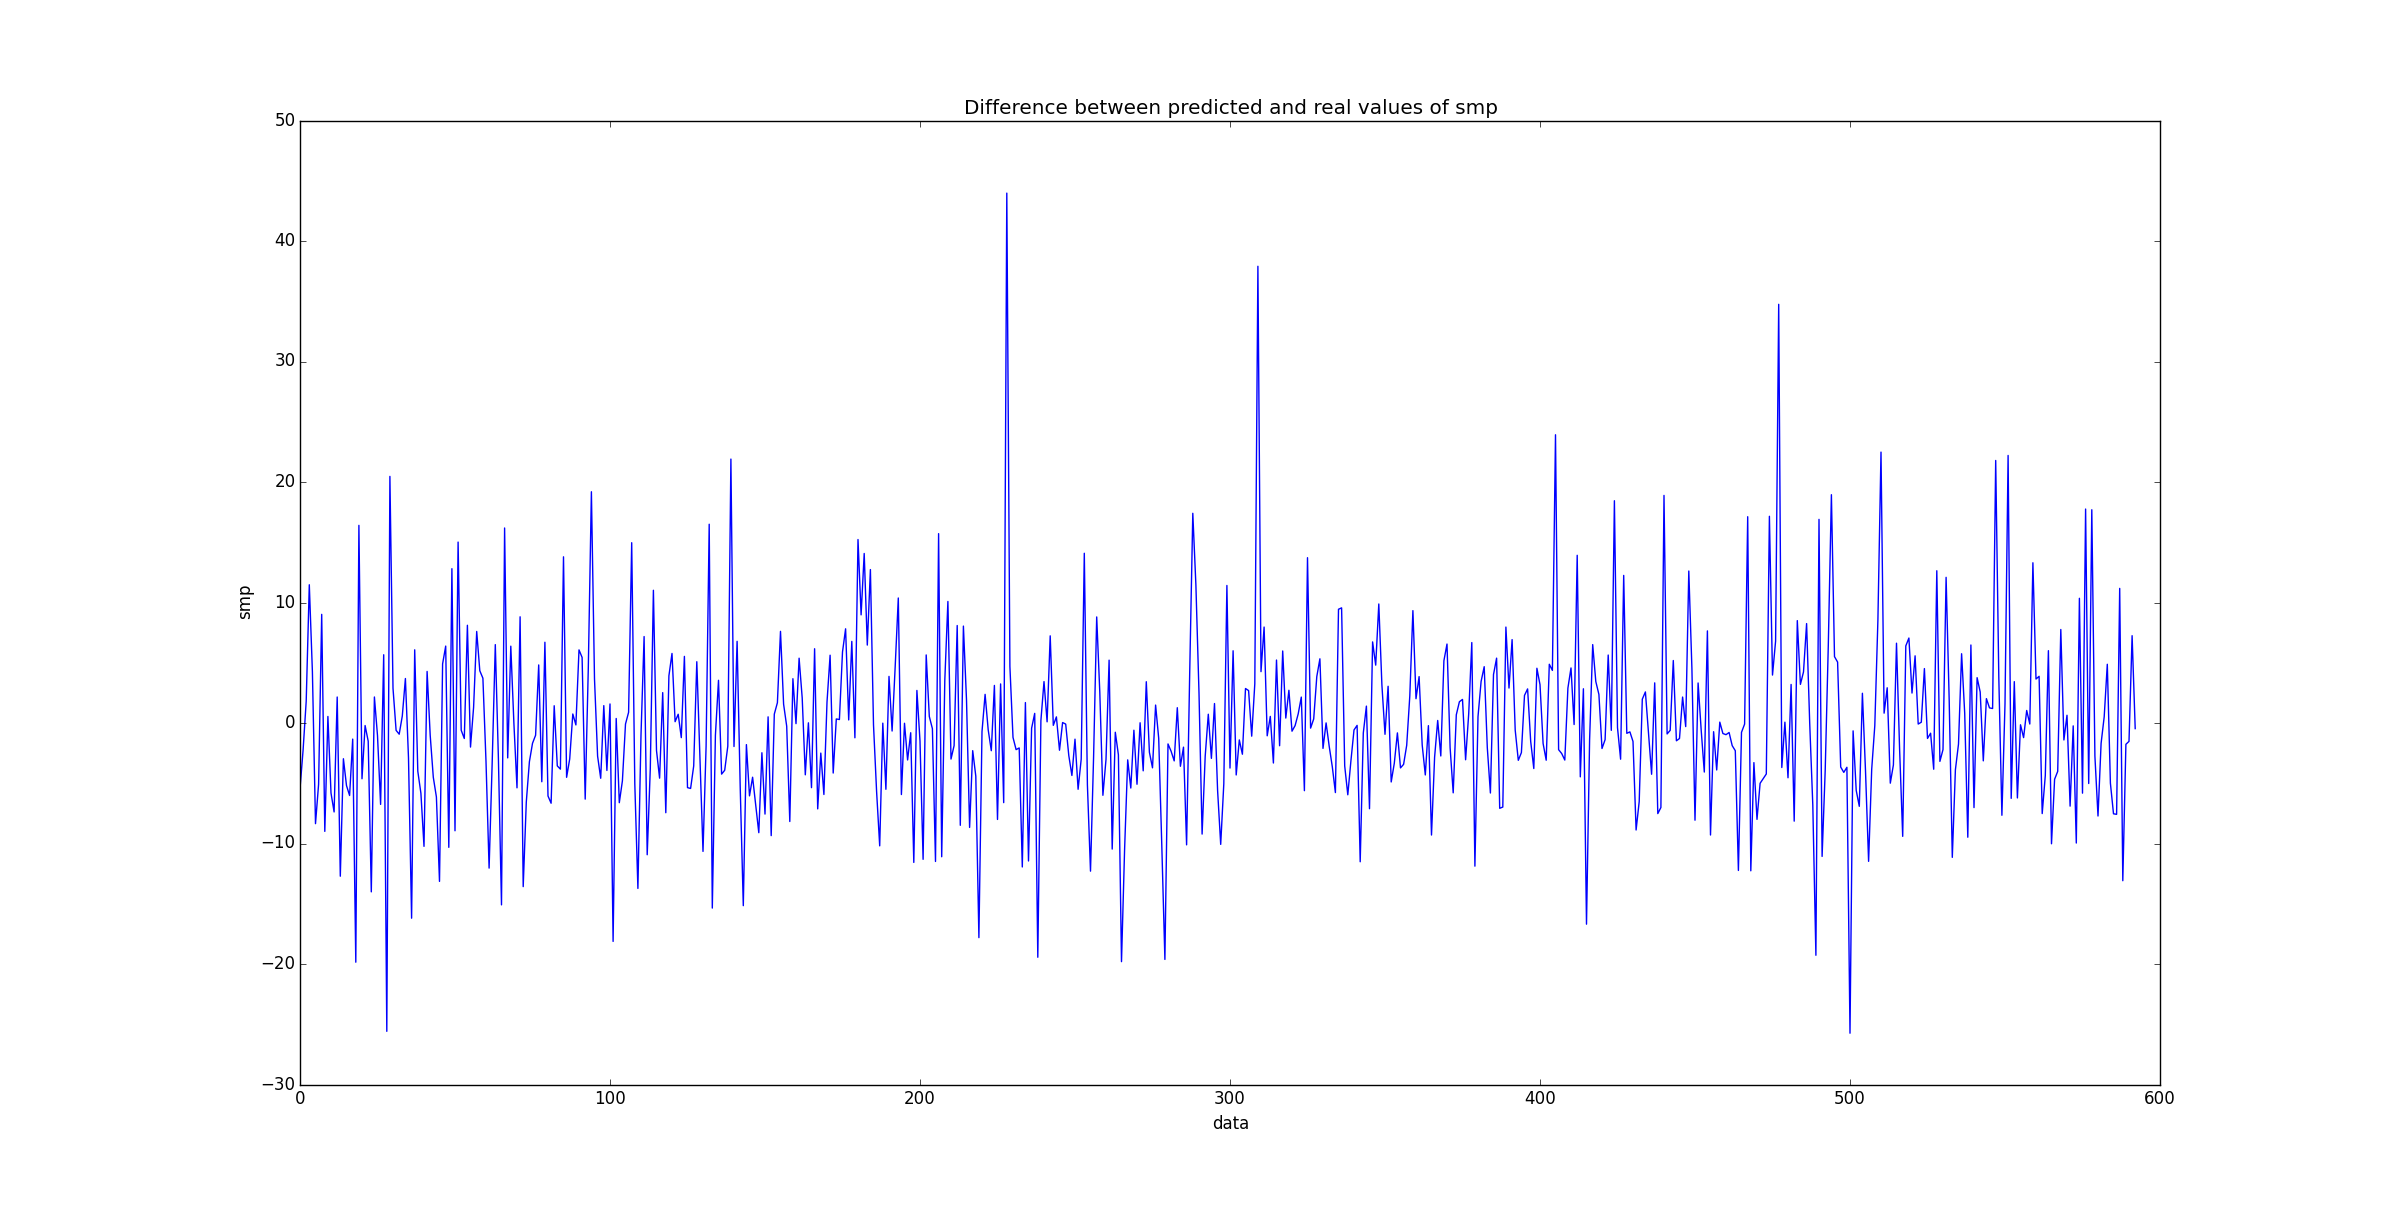
\includegraphics[width=1.4\textwidth]{fig/rf_smp_y2.png}}%
  \caption{\tl{Random Forest}: ������� \tl{real-expected} ����� ��� \tl{SMP}}
  \label{figure:12}
\end{figure}

\begin{minted}[linenos]{python}
import matplotlib.pyplot as plt
plt.figure()
plt.plot(smp_test-y1)
plt.xlabel('data')
plt.ylabel('smp')
plt.title('Difference between predicted and real values of smp')
plt.show()
\end{minted}

�� ���������� ����� ���� ����� ��� ���������� ��� ����������� �����. ���� �������� ��� �� ������� ��� ������ �� ������ ����� �����, ���� ���� ��� 5 ������� ��� �� ����������. ����������� �� ������ ������ ������� ��������, �� ������ ����������� ��� �� ������� ��� �� ���� �� ������ �� \tl{SMP} ������� ������� ����� ��� �� ������� ��� ��������� ���������� ��� ������������� ���������� ������ ������.

\newpage
\subsection{\tl{Feature Importances}}

�� ����� ����� ���������� ������� ��� ��� ��������� ���� ���� ��������� ��� ������������� ��� ����������.  

\begin{figure}
  \makebox[\textwidth][c]{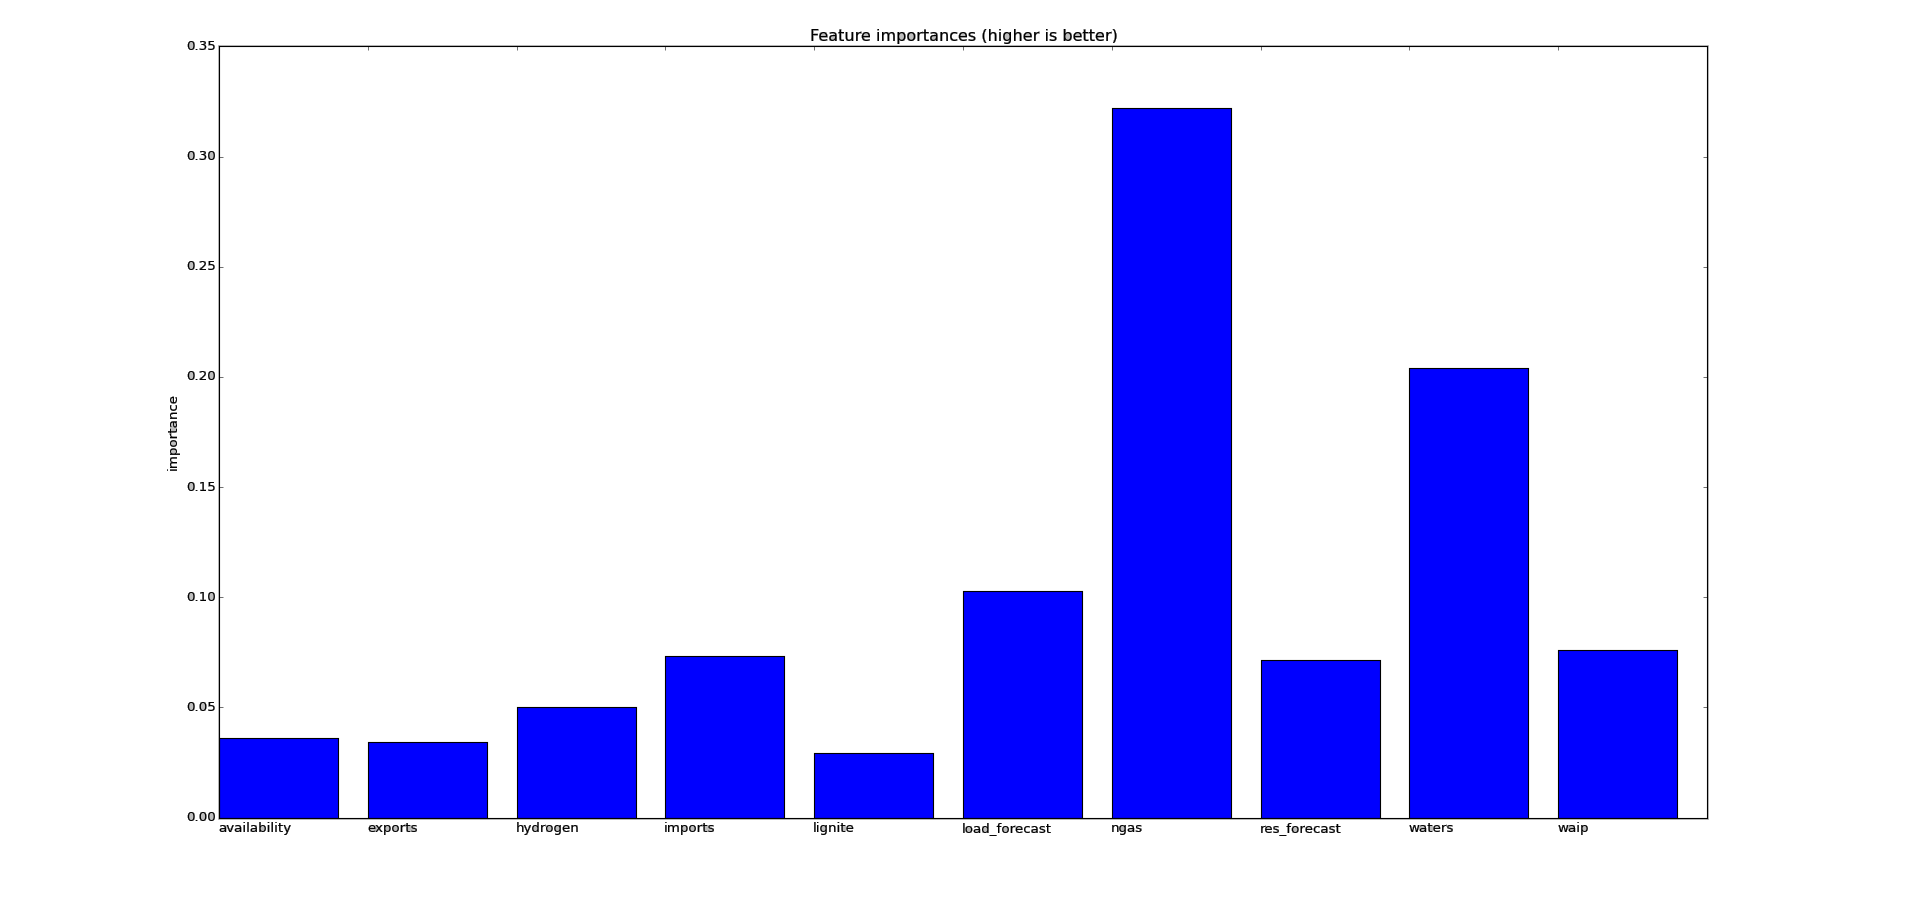
\includegraphics[width=1.4\textwidth]{fig/rf_feature_importances.png}}%
  \caption{\tl{Random Forest: Feature Importances}}
  \label{figure:16}
\end{figure}

\begin{minted}[linenos]{python}
fi = enumerate(rf.feature_importances_)
df2 = df.drop('smp', 1)
cols = df2.columns
print [(value,cols[i]) for (i,value) in fi]
features = mlab.csv2rec(path + 'rf_features.csv',delimiter=',')
plt.figure()
plt.bar(np.arange(len(features)),features['value'],label='values')
plt.xticks(range(len(features)),features['feature'], ha = 'left')
plt.ylabel('importance')
plt.title('Feature importances (higher is better)')
plt.show()
\end{minted}
\newpage

\begin{table}[h!]
\centering
 \begin{tabular}{||c c||} 
 \hline
 \tl{Feature} & \tl{Importance} \\ 
 \hline\hline
 \textlatin{availability} & 0.0361405 \\ 
 \hline
 \textlatin{exports} & 0.0344914 \\
 \hline
 \textlatin{hydrogen} & 0.0502056 \\
 \hline
 \textlatin{imports} & 0.0733868 \\ 
 \hline
  \textlatin{lignite} & 0.0292468 \\ 
 \hline
  \textlatin{load\_forecast} & 0.1026408 \\ 
 \hline
  \textlatin{ngas} & 0.3220485 \\ 
 \hline
  \textlatin{res\_forecast} & 0.0717241 \\ 
 \hline
  \textlatin{waters} & 0.2040629 \\ 
 \hline
  \textlatin{waip} & 0.0760525 \\ 
 \hline
\end{tabular}
\label{table:2}
\caption{\tl{Random Forest}: �������������� ���������������}
\end{table}

�� ��� ��������� �������������� ���� ��������� ��� ������ ����� �� \tl{ngas} ��� ������ ������� �� \tl{waters}. ���� �� ��� �������������� ���������� ��� ������ ����� �� ������� ���������� ��� 50\%. ������ ��������� ���� �������� �� ���� ��� �� \tl{load forecast} �� ����� ��������� �� ������� 10\% ��� ���� ��� \tl{SMP}. �� ��������� ���������� ������� ���� ������ ��������� ��� ������, ���� �� ��������� �������. 

\section{\tl{CART (Regression Trees)}}

\subsection{�������� ���������}

�������� ��� ��������� ��� \tl{regression trees} ��� ���� ��� 1 ��� 20 ���� �� ����� ���� ����� �� �������� ����� ��� �� ����� �� ������� ������������.

\begin{minted}[linenos]{python}
from sklearn import tree
from sklearn import metrics as skm
train_acc = test_acc = exp_var_score = mae = mse = np.zeros(20) 
for i in range (1,21):
    tr = tree.DecisionTreeRegressor(max_depth=i)
    tr.fit(dataset_train, smp_train)
    tr.get_params()
    y1 = tr.predict(dataset_test)
    train_acc[i-1] = tr.score(dataset_train, smp_train)
    test_acc[i-1] = tr.score(dataset_test, smp_test)
    exp_var_score[i-1] = skm.explained_variance_score(smp_test, y1)
    mae[i-1] = skm.mean_absolute_error(smp_test, y1)
    mse[i-1] = skm.mean_squared_error(smp_test, y1)
\end{minted}

\begin{figure}
  \makebox[\textwidth][c]{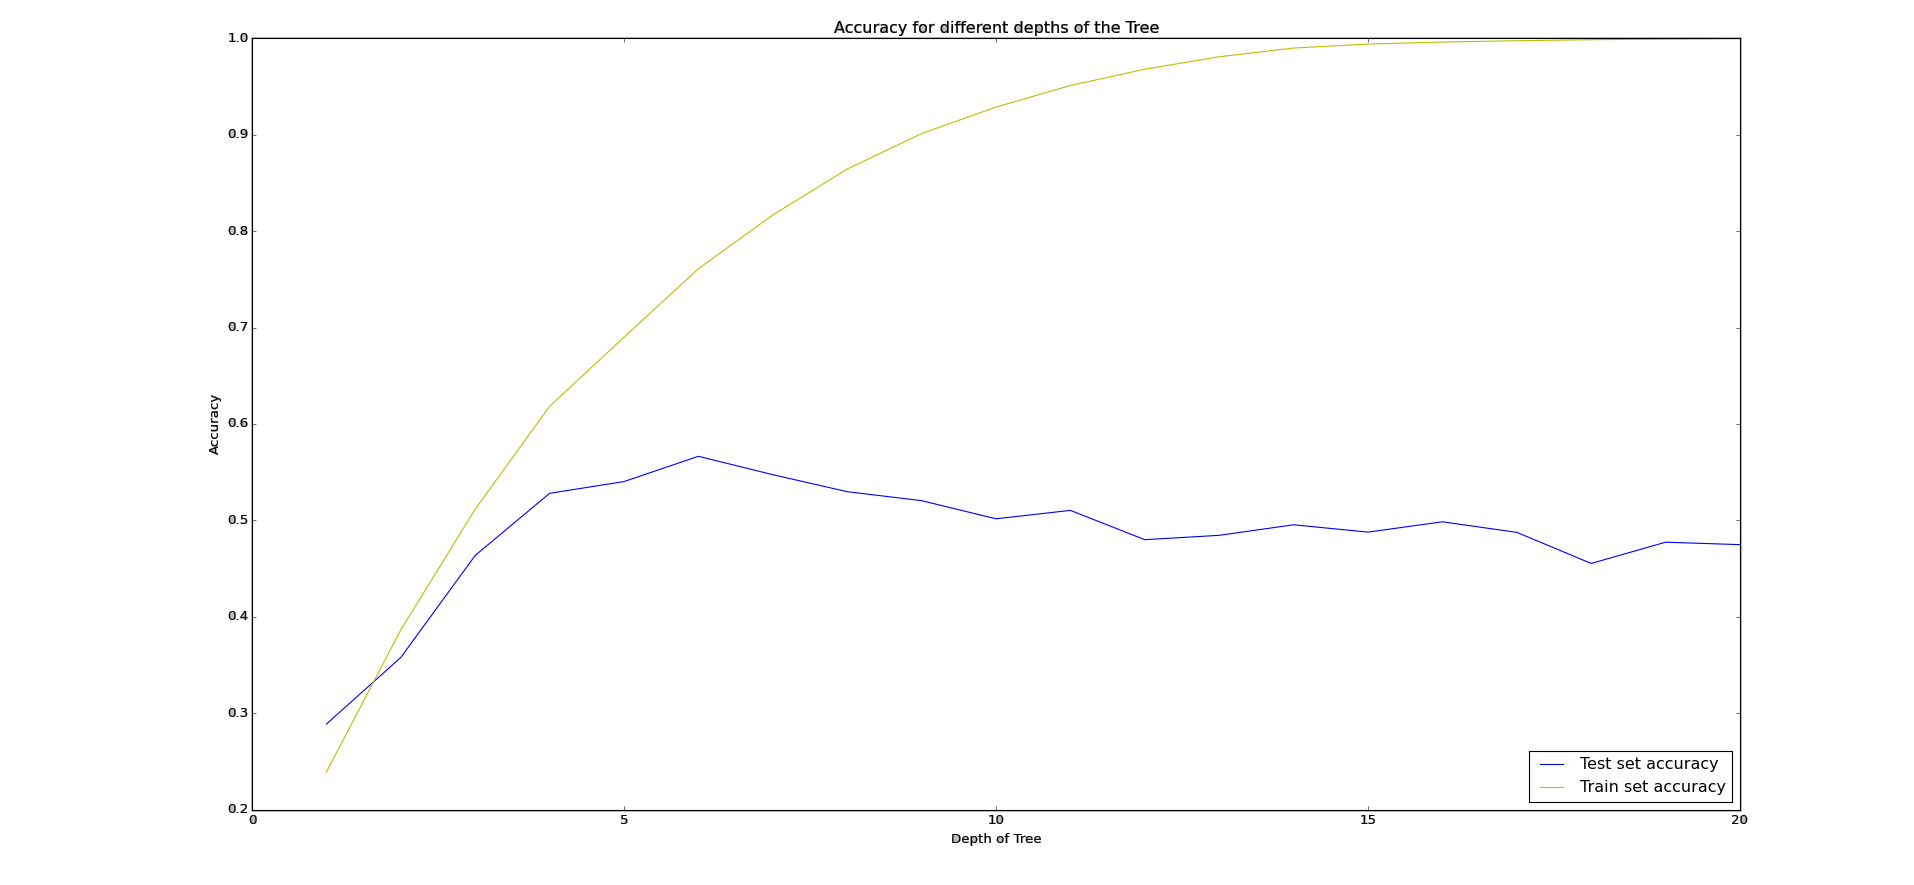
\includegraphics[width=1.4\textwidth]{fig/accuracy_tree.png}}%
  \caption{\tl{Tree Regressor: Accuracy}}
  \label{figure:17}
\end{figure}

\begin{figure}
  \makebox[\textwidth][c]{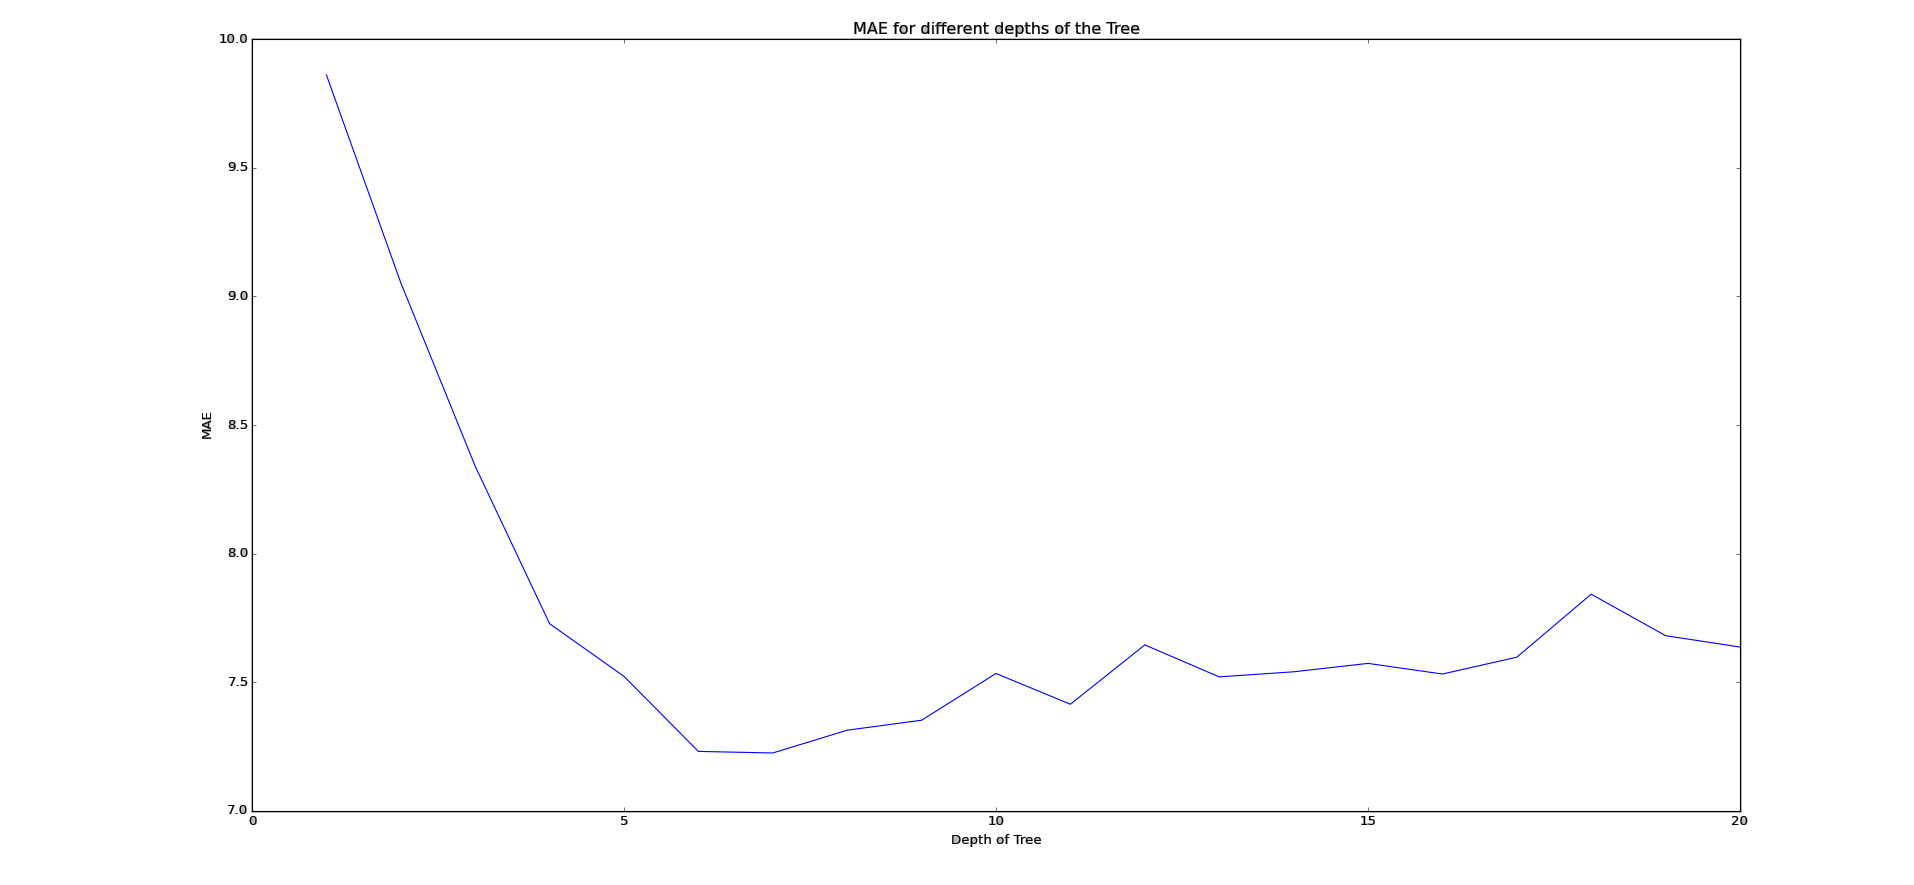
\includegraphics[width=1.4\textwidth]{fig/mae_tree.png}}%
  \caption{\tl{Tree Regressor: Mean absolute error}}
  \label{figure:18}
\end{figure}

\begin{figure}
  \makebox[\textwidth][c]{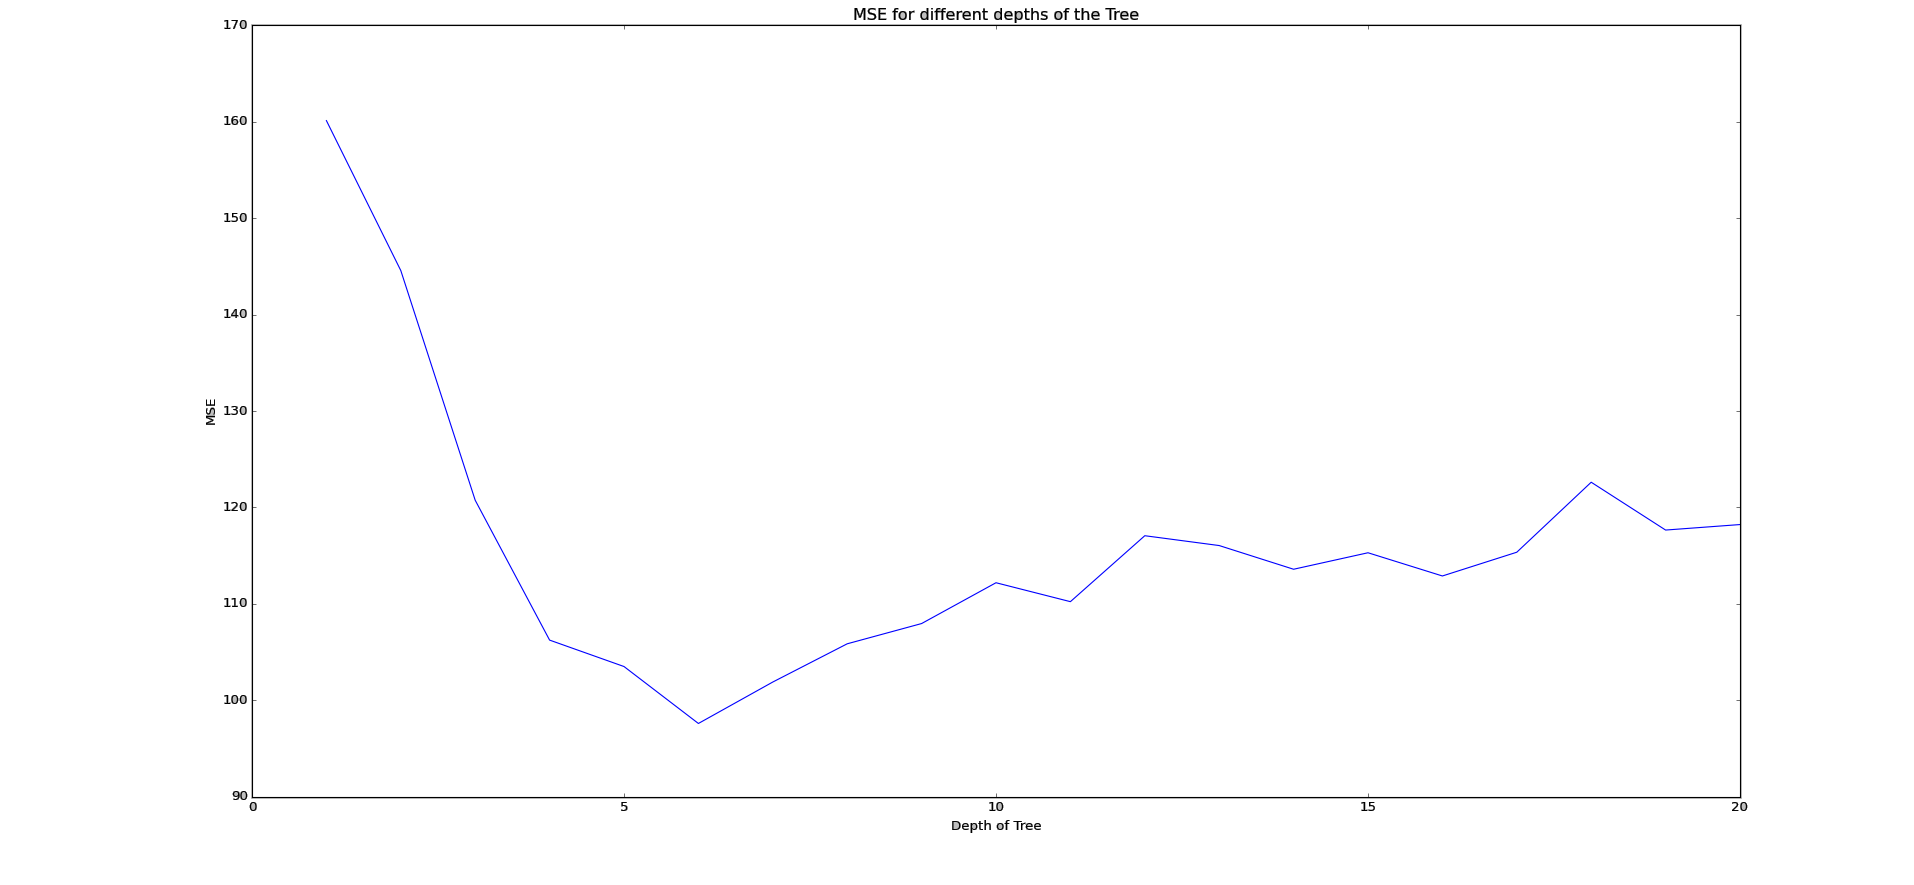
\includegraphics[width=1.4\textwidth]{fig/mse_tree.png}}%
  \caption{\tl{Tree Regressor: Mean squared error}}
  \label{figure:19}
\end{figure}
\newpage
�� �������� �� ����, � ���������� ��� ���� ���� ����� ���������, ��� ������ ������� �������� ��� 54,75\% ��� ������ ������ 6. ��� ��������� �� ����� � �������� ��� �������, ������� ������� �� ����� �������� ��� ������ \tl{overfitting} ��� �������. ��� ����� ������� ��� �� \tl{max\_depth} �� ���������� ��� ��������� ����� ���� ���� ��� 50\%. �� ���� �������� ��� �� ������������ ��� \tl{MAE} ��� \tl{MSE}, �������� � ������� �� ����� ��� ������ ������ 6.

\subsection{\tl{Cross Validation}}

���� ��� ��� \tl{random forest}, �������������� \tl{cross validation} ���� �� ������������ �� ������������ ���. �� ������������ ����� ���� �� ������������.\\

\tl{5-fold Cross Validation Scores}: \\
$\left [  0.57645212 \; \; \;  0.55334927 \; \; \; 0.64557411 \; \; \; 0.6136979 \; \; \; 0.54650035
\right ]$ \\
\tl{Cross Validation Accuracy}: 0.59 (+/- 0.02) \\

\tl{10-fold Cross Validation Scores}: \\
$\left [  0.64172542 \; \; \;    0.42875275 \; \; \;  0.53303435 \; \; \;  0.59282483  \; \; \; 0.67429731 \; \; \;   0.59046097 \right.$ \\
 $ \left. 0.64643966 \; \; \;  0.52166911; \; \;   0.60511882 \; \; \;  0.3935244
\right ]$ \\
\tl{Cross Validation Accuracy}: 0.56 (+/- 0.04) \\

\subsection{����������� - ������������ ����� \tl{SMP}}

��� ����� \ref{figure:20} �������� ��� ������� \tl{real} ��� \tl{expected} ����� ��� �� \tl{SMP} ������� �� �� ��� ��������� ��� \tl{regression trees}.

\begin{figure}
  \makebox[\textwidth][c]{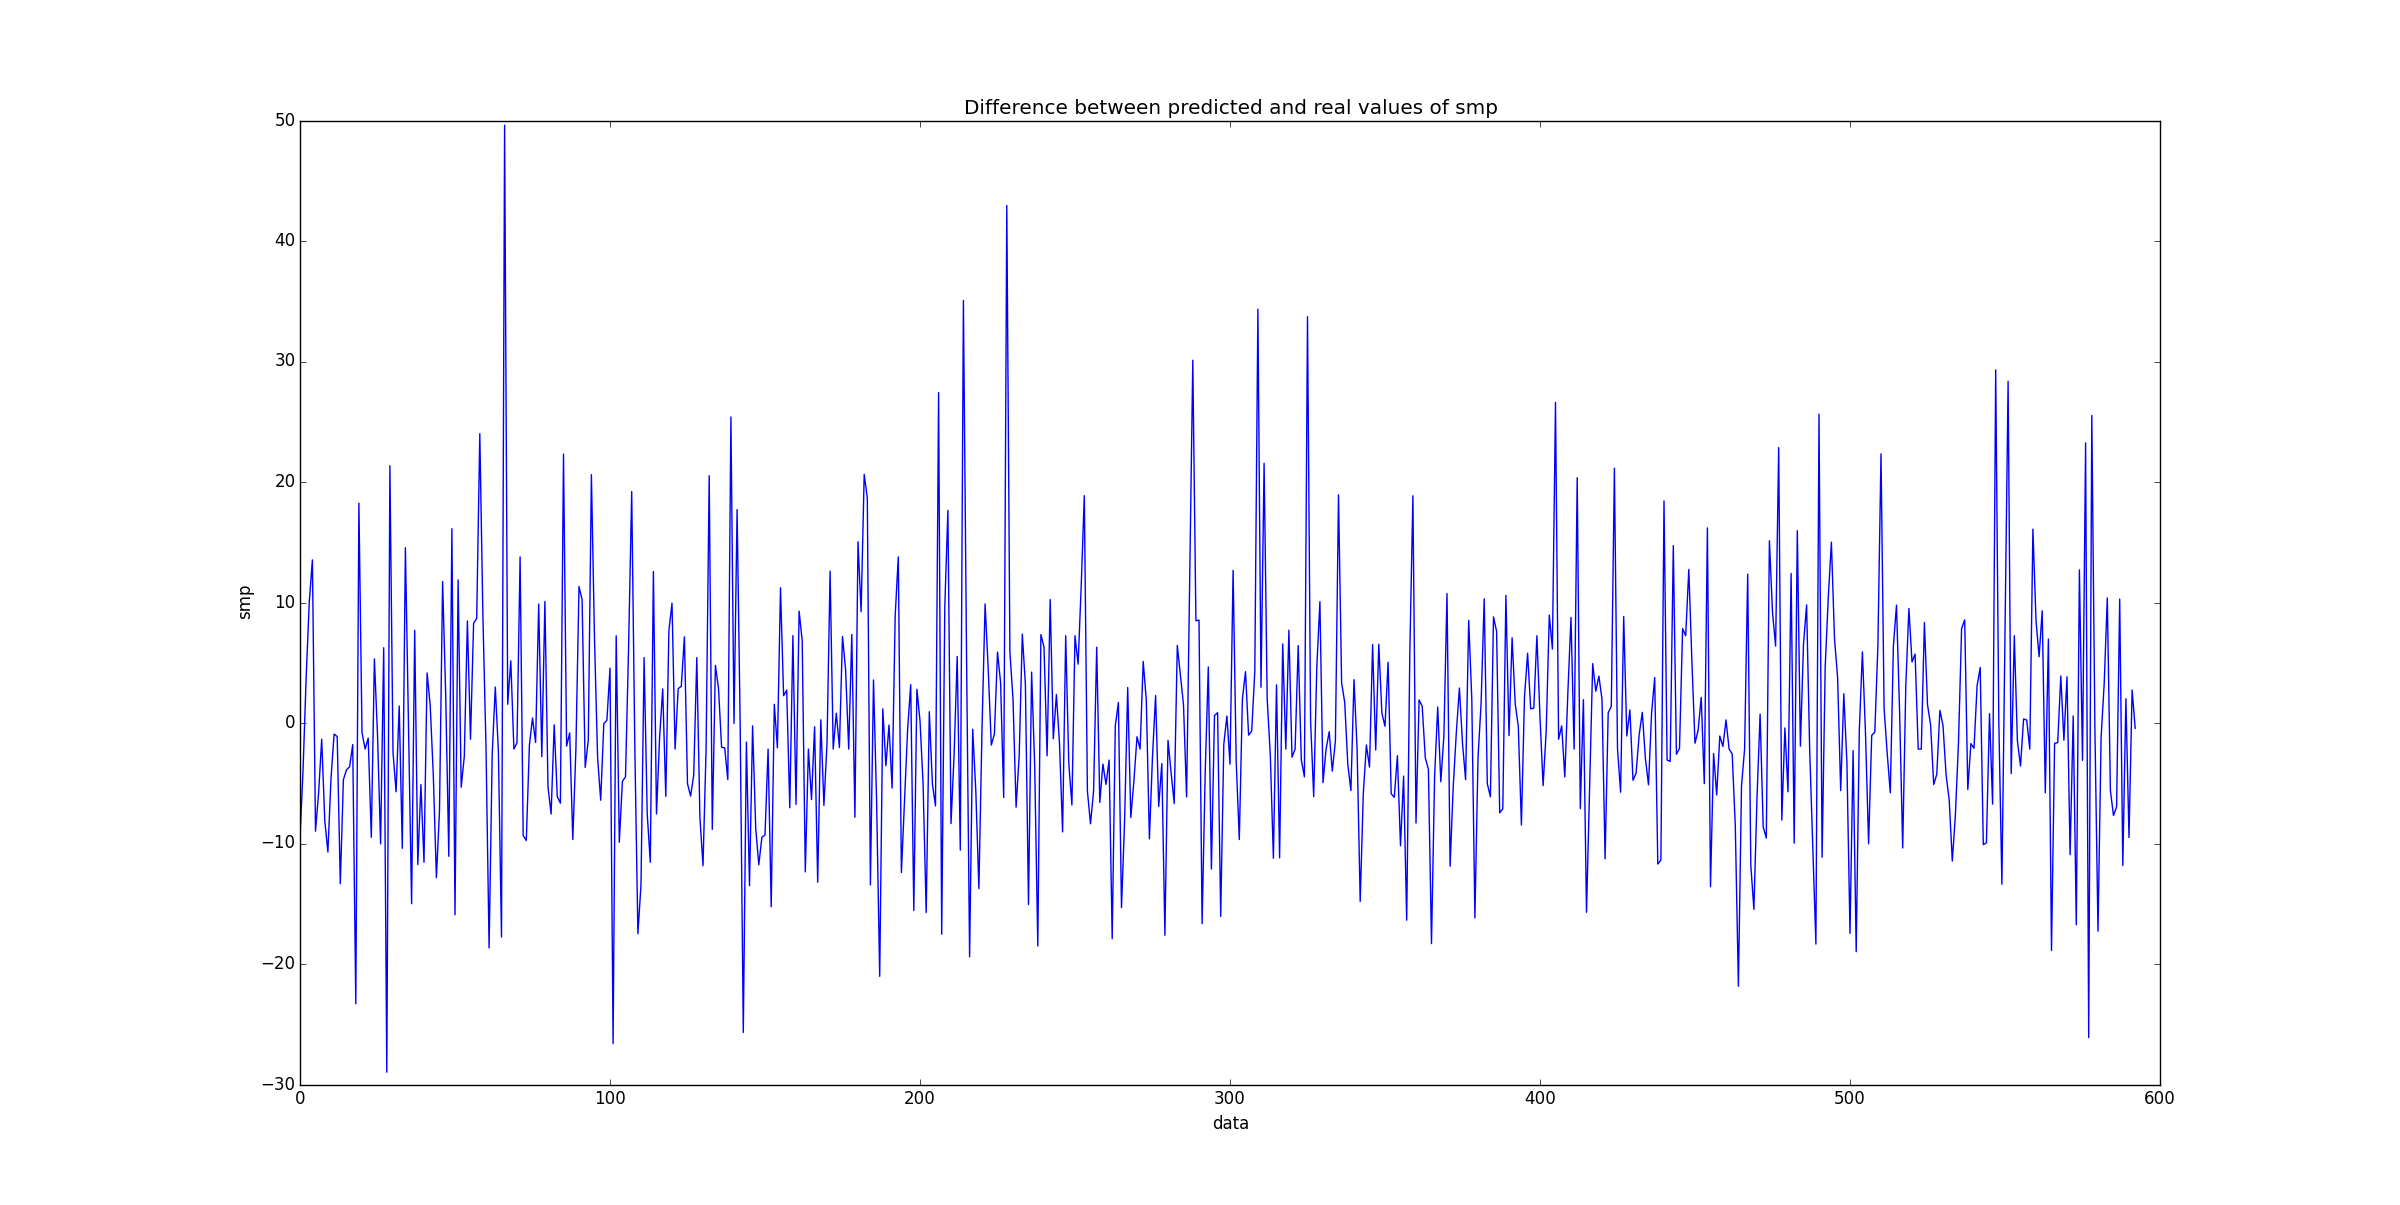
\includegraphics[width=1.4\textwidth]{fig/tree_smp_y2.png}}%
  \caption{\tl{Tree Regressor}: ������� \tl{real-expected} ����� ��� \tl{SMP}}
  \label{figure:20}
\end{figure}

����� ������� � ������� ���� �������� �� ����� �� ��� ��������� \tl{random forest}. ������ ���������� �������� ��� ��� ����������� ����� �� �������� �� ������. ������ �������� ��� �� ������� ��������� �� ��������� ������� �����, ������� ����� ������� �����.

\subsection{\tl{Feature Importances}}

\begin{figure}
  \makebox[\textwidth][c]{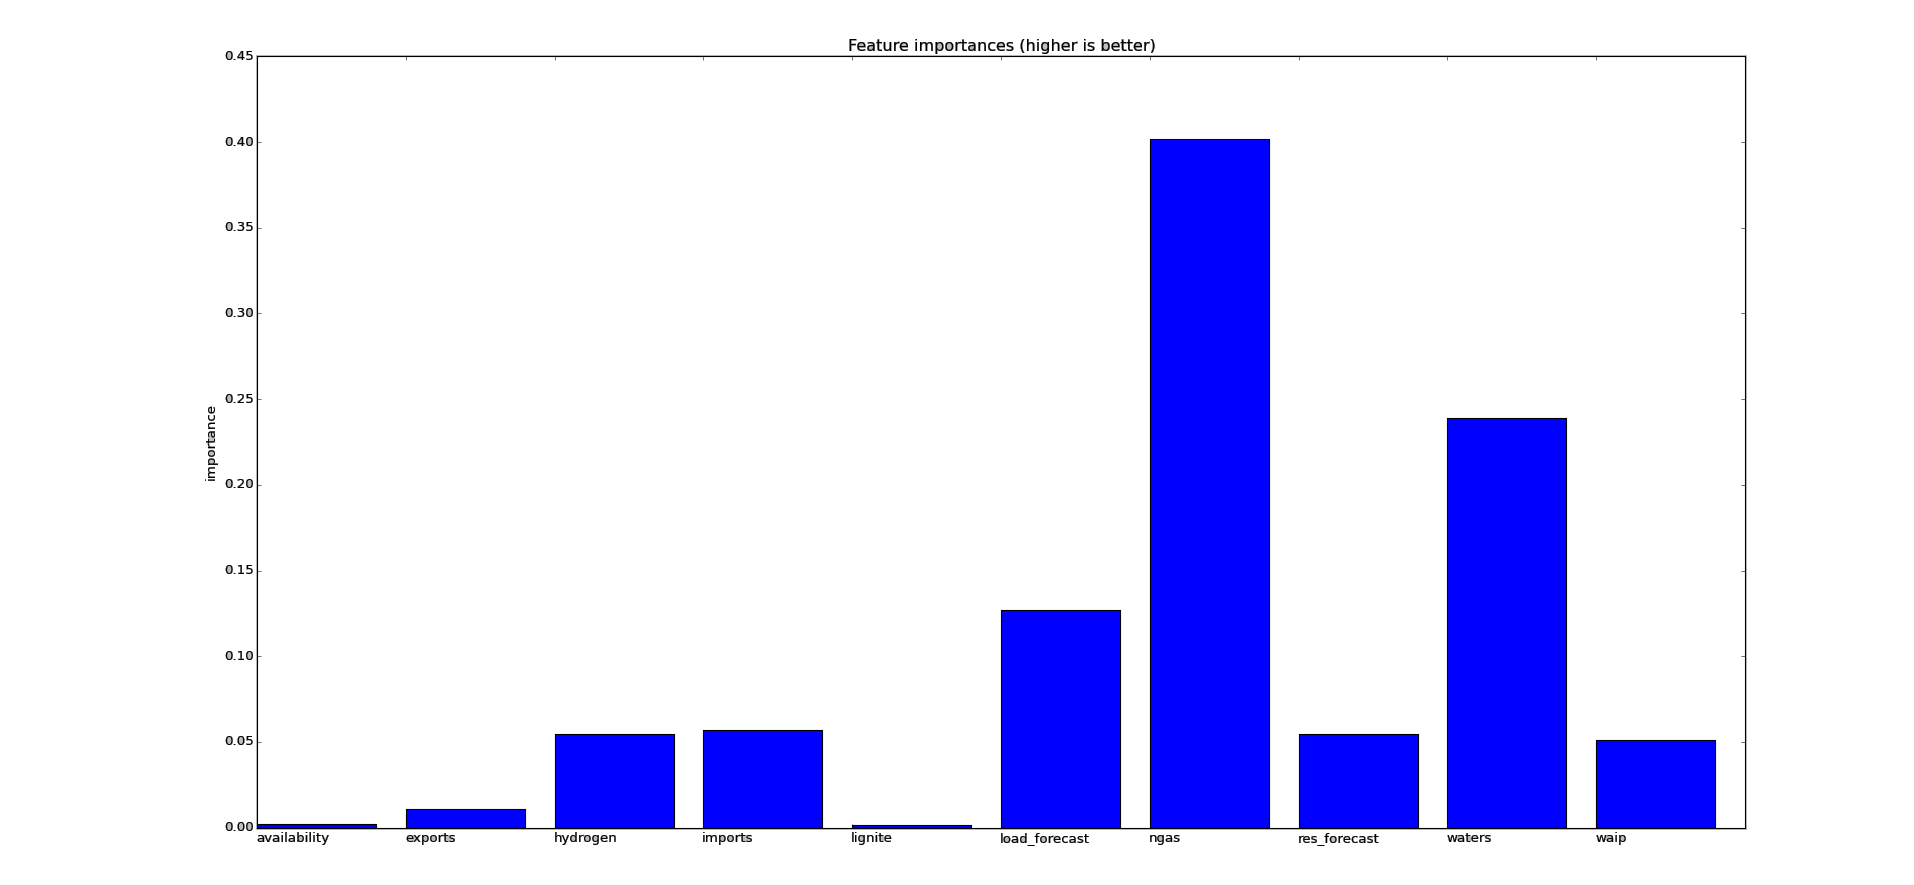
\includegraphics[width=1.4\textwidth]{fig/tree_feature_importances.png}}%
  \caption{\tl{Tree Regressor: Feature Importances}}
  \label{figure:21}
\end{figure}

\begin{table}[h!]
\centering
 \begin{tabular}{||c c||} 
 \hline
 \tl{Feature} & \tl{Importance} \\ 
 \hline\hline
 \textlatin{availability} & 0.0023202 \\ 
 \hline
 \textlatin{exports} & 0.0111215 \\
 \hline
 \textlatin{hydrogen} & 0.0548785 \\
 \hline
 \textlatin{imports} & 0.0570344 \\ 
 \hline
  \textlatin{lignite} & 0.0013275 \\ 
 \hline
  \textlatin{load\_forecast} & 0.1269267 \\ 
 \hline
  \textlatin{ngas} & 0.4016380 \\ 
 \hline
  \textlatin{res\_forecast} & 0.0545563 \\ 
 \hline
  \textlatin{waters} & 0.2391213 \\ 
 \hline
  \textlatin{waip} & 0.0510756 \\ 
 \hline
\end{tabular}
\label{table:2}
\caption{\tl{Tree Regressor}: �������������� ���������������}
\end{table}

� ���������� \tl{CART} ������ ��������� �� �������������� \tl{ngas} �� ������� 40\%, ����������� ��� ��� ���� ��������� \tl{random forest}. �� ���� ��������� ��� �� �� �������������� \tl{waters} ��� \tl{load\_forecast} �� ����� ����� ���������� ������������� �� ����� �� ���� ��� ����� ��� \tl{random forest}. �� �������� �������������� �������� ��� ������� ��������� ����, ������� �� \tl{lignite} ��� \tl{availability} ����� �������� ������� ��� ������ ����������. 
\newpage
�� �������� ���������� ��� ������� ��� ��� ��� ��� ������ �� ������ ��� ���� ����� �����, �������� ����� ������ �� ������� ��� ��������������� �� ����� ���������, ��� ��� ���� ��� ������ �� ���������� �� ���� ���� �������� ���� ������� ��� \tl{random forest} ���� �������������� ����������� ��� �� �� ������� ��� ��� �������������� ��� ����������. \newpage
����������� ��� ���������� ��� ��� ���� ���� ��������� ��� ������ ����������� ��� �� �������������� �� ������ �����, ���� ����� ���� �������� �� ������ �� \tl{ngas}. ������ ����� ������� ��� � ���������� \tl{random forest} ������������� ��� ���� ��� ������� ���� ��������� \tl{CART} ��� ������� ����� �� ���� ���������� ��������, ������ ��� �������� �� ��� ��������� ���� ��������� �������.

\subsection{������ ������}

������������ �� ������ ��� �� ������� ������� �� ������ .\tl{dot} ��� ������ �� ��������� ���� ��� \tl{Graphviz}.  

\begin{minted}[linenos]{python}
sklearn.externals.six import StringIO
with open(path+"tree_3.dot", 'w') as f:
    f = tree.export_graphviz(tr, out_file=f)
\end{minted}

\begin{sidewaysfigure}
  \makebox[\textwidth][c]{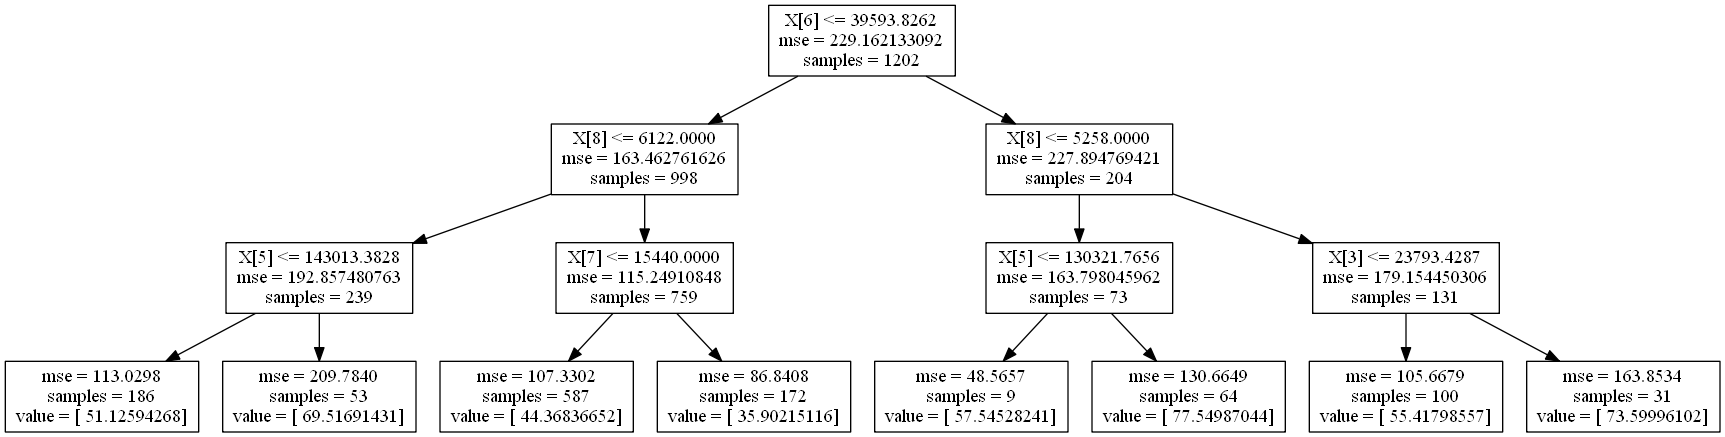
\includegraphics[width=\textwidth,height=\textheight,keepaspectratio]{fig/tree_3.png}}%
  \caption{������ ���������� \tl{Tree Regressor} - ����� 4}
  \label{figure:22}
\end{sidewaysfigure}

������ �� ������ ���� ���� ������ ��� �� ������������ ���, ��������� ���� ������� ��� ����� 5 ��� 6 ��� ����� ������ ������������� �� ���������� ��� ������ ������ 4 �� ����� ����� \tl{mean accuracy score = 0.463656}. �� ���������� ��� �������� ��� ������ ����� �� ����:
\begin{itemize}
\item $X\left [ 3 \right ]$ : \tl{imports}
\item $X\left [ 5 \right ]$ : \tl{load\_forecast}
\item $X\left [ 6 \right ]$ : \tl{ngas}
\item $X\left [ 7 \right ]$ : \tl{res\_forecast}
\item $X\left [ 8 \right ]$ : \tl{waters}
\end{itemize} 

�� ���� ����� ��� ������� ������ 3 ��������������: �� ����� ��� ����������, �� \tl{MSE} ��� ��� ������ ��� ��������� ��� �������� ���� ������������ �����. ������ �� \tl{training set} �������� �� 66.6\% ��� ������� ���, ������ ������ 1202 ��������. ������� �� �� �� ������ � ������� ��� ������������ ���� ���� ����� � ��� ���� ��� ���������� �����, ��� �������� �� � ������� ����� ������ ��� ��� ����� �� ��� ����� (�� �������� ����� ��� ������ $X\leq \alpha$ �� ����� ���������� �� $X>\alpha$ �� ��� ��� ���� ����� ��� ��� ���� ��������). �� ������ ����� �������.

� ��������� \tl{ngas} ��������� ��� ����� ���� ����� �� ����� \tl{partition}, ������������� ��� ��� ��������� \tl{waters}. �� \tl{load\_forecast} �� ����� ������������� ����� 2 \tl{partitions} ��� ������� 3. ����������� ��� �� ���� ���� �� ������ ��� ��������� �� ��� ��������� ��������, ���� ����������� �� ��� �������� ����� ��� 3:1. �� ���������� ������������ �� ����� �������������� �� ���� �������, ��� ������� (������ ��� �������� ��� �����) �� ���������� ���� �� ��� ���������� ���������� ������������ �������� (��� ���������� �� \tl{ngas} ����������� ���� ��� ����� 4 ��� �� \tl{lignite} ����������� ������ ��� ����). ��������� ������ �� ������� ��� �������������� ���� 5 ��� ��� 10 ���������� ��� �������� 46\% ��� �� ����� 6 �� �������� 56\% ���������������� ���� �� ���������� �� ����� ������������ ��� ��� �� �������������� ��� �������� ����������� ���� ��������� ��� ������.
\newpage
\section{\tl{MARS}}

��� �� ������� \tl{MARS} ��������������� � ���������� \tl{pyearth} ��� ����������� � \tl{Jason Rudy} � ����� ��������� ��� ��������� ��� ����������� ��� ��� \tl{Jerome Friedman} ��� ������������� ��������� ��� �������� 3 (\citealpsec{pyearth}). 

\begin{minted}[linenos]{python}
from pyearth import Earth
model = Earth()
model.fit(dataset_train,smp_train)
print model.trace()
print model.summary()
\end{minted}

\subsection{\tl{Forward Pass}}

��� ����� \ref{figure:23} ������������� � ����� ���� ��� ����������, ���� ������������� �� ������� ������������ ����������� �����. � ������ ��� ��������� ����� � $h_0(X)=1$. �� ���������� ��� ���������� ��� ����������� \tl{var}, \tl{terms} ����� � ������� ��� ����������� ����� ��� ������ ������� ����� �� ������������ \tl{iteration} ��� ����������, \tl{gcv} ����� �� �������� \tl{Generalized Cross Validation}, \tl{rsq} ����� �� $R^2$ ��� �������� ��� \tl{grsq} ����� ��� �������� ��� ������������ ���������� ��� ��������.  

\begin{figure}
  \makebox[\textwidth][c]{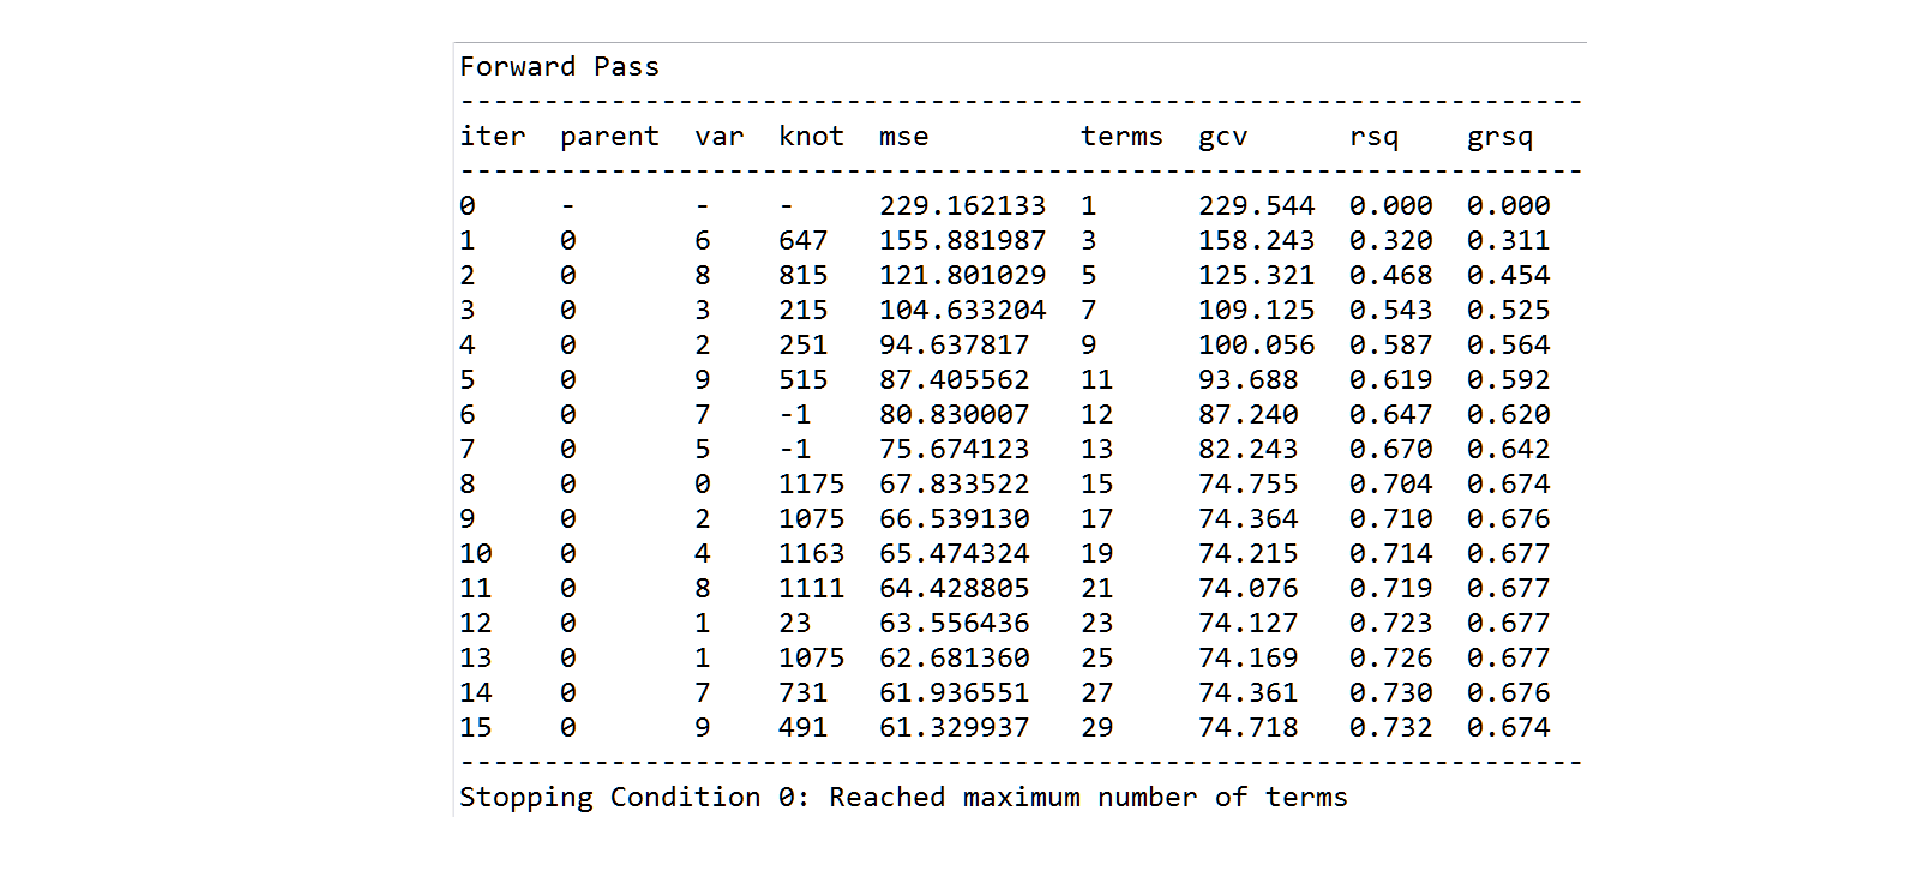
\includegraphics[width=1.4\textwidth]{fig/forward_pass.png}}%
  \caption{\tl{MARS: Forward Pass}}
  \label{figure:23}
\end{figure}

���� ��� ����� ������������� ����������� ��� �����������, � ��� ��������� ��������� ����� �� \tl{ngas} ������������� ��� �� \tl{waters}. �� ��� ���������� ���� ��� ������ ����������� ��������� ��� 45,4\%. ���������� ����������� �� ������� ��� �� �������� ����� ���������� ��� ��� ������ �������������� ����������� ������ ����� �� \tl{imports}, \tl{hydrogen} ��� \tl{waip}. ����������� ��� ��� ��������� ��� ������������� ��� �������� ���� ��������� ����� �� \tl{MSE} ��� �� ���������� \tl{gcv, rsq} ��� \tl{grsq} �������� �� ��������� �����. ���� ��� ����� ���� ��� ���������� ��������� ����� \tl{gcv} = 74.71,  $R^2 = 0.732$ ��� \tl{grsq} = 0.674, ����� ���� ����� ���� ����������� ��� ������ ���� �� ��� ��������� \tl{Random Forest}.

\subsection{\tl{Pruning Pass}}

� ������� ���� ��� ���������� ������� �� ��� ���������� ���������� ����������. ������ ����� �� ���������� ����������� ��� ���������� �������� ��� ���� ���� \tl{fit} �� ����� �� �������. � ���������� �� �������� �� \tl{iteration} ��� ������������� �� \tl{gcv}, �� ����� ��������� ���� ������ ���������. ���� ���� ��������� ������ ��� �� ������� \tl{grsq}, �� ����� ��� ������� �� ����������������. �������� �� ������ ��� ������� �� ���� 10 ���������� ����� �� ����� �� �� ������, ��� �� ����� �� �������� ������� ��� ������ �� ������� � ����������.

\begin{figure}
  \makebox[\textwidth][c]{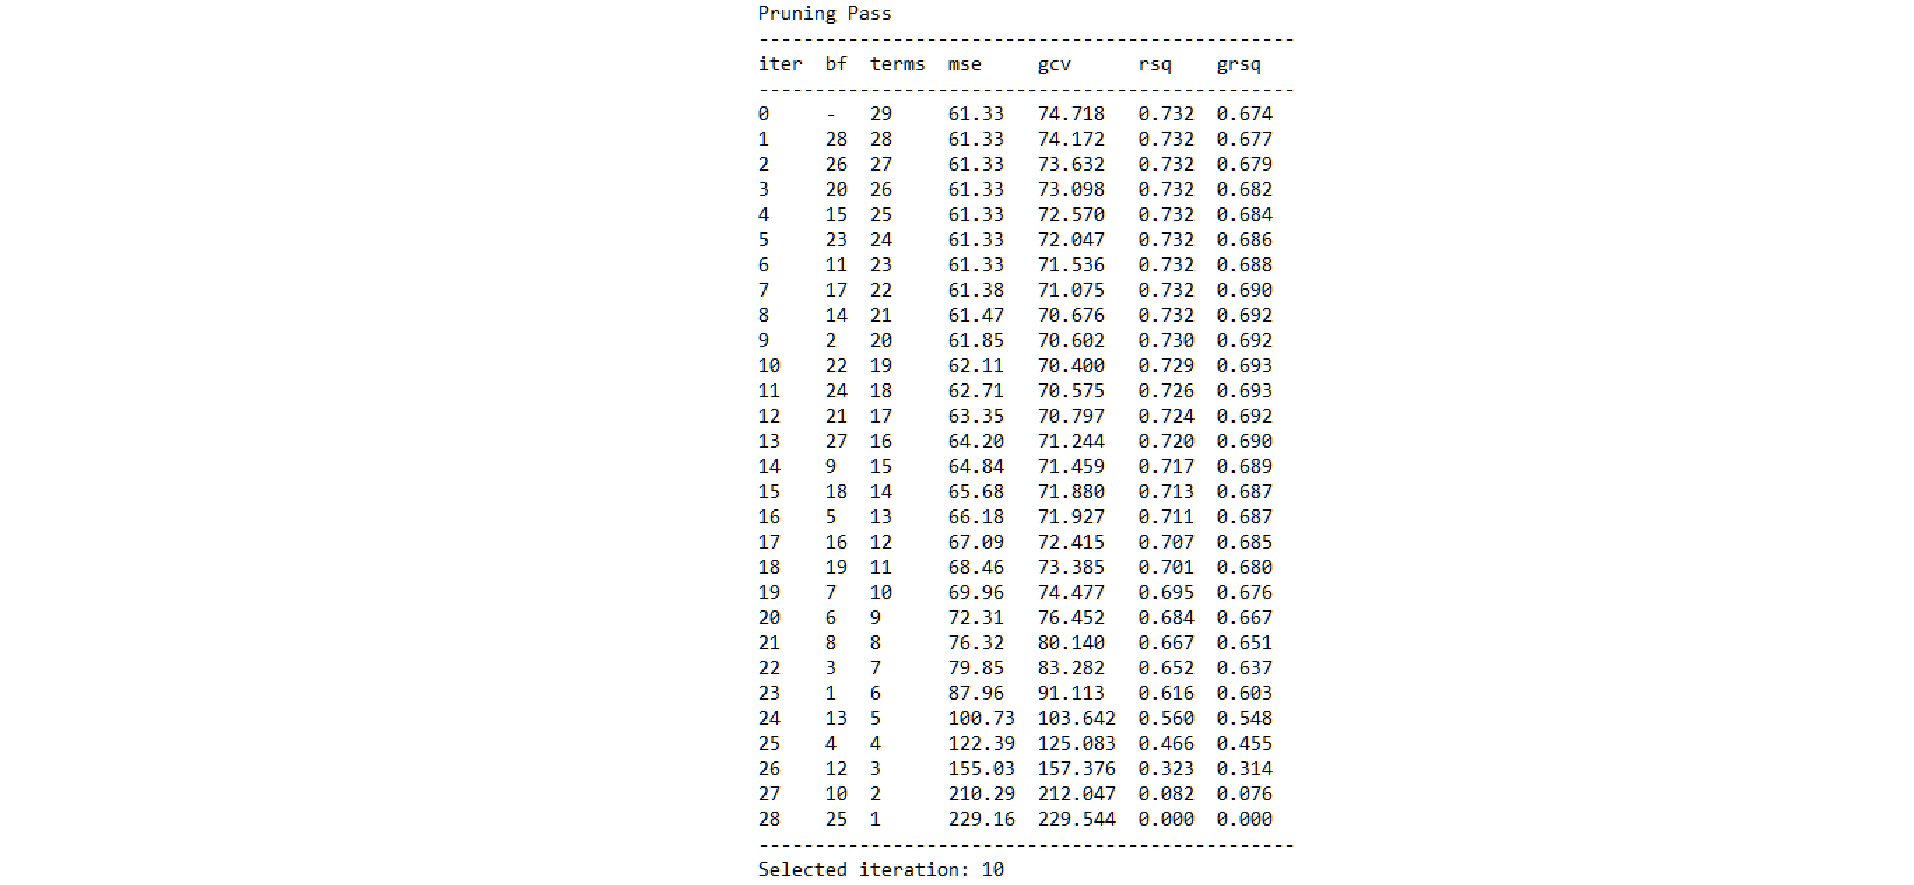
\includegraphics[width=1.3\textwidth]{fig/pruning_pass2.png}}%
  \caption{\tl{MARS: Pruning Pass}}
  \label{figure:24}
\end{figure}

\subsection{������ �������}

��� ����� \ref{figure:24} �������� �� ������ ������� ��� ����������. � ����� ����� �������� ���� ��� ����������� ������ ��� �������������� ���� �� \tl{forward pass}, � ������� ����� ��� ���� ����� ��� ����� ��� ����������� ����������� ��� � ����� ����� ��� ������� ����������� ������� �� ��� ���������� ��� ���� ����������. ����������� ��� ��� �� ��� ��� ����������� ����� ��� ���������� \tl{ngas} ����������. �� ��������� ������� ����������� ������� �� ����� ���� �� ������� �������. �� ������ ������������ ��������� ���� ��������� ������. � ���������� ��� ������ �� ���������� �� ������� ����� ��� 70\% ��� �����, ��� ���� ���� �������.

\subsection{����������� - ������������ ����� \tl{SMP}}

��� ����� \ref{figure:26} ������ �� ��������� �� �� ������� ����������� ��� \tl{expected} ����� ��� \tl{SMP}. �� ������� ������� ������� �������� ������������ �� ����� �� �� ���������� ��� �������� \tl{CART} ��� ����� ���������� �� ������� �� �� ������� \tl{Random Forest}. ������� �������� ������ ��� �� ���������� ��� �������� ����� ��������� ��� ��� \tl{Random Forest} �� ��������� ������ ��� ������ ������ ��� �� ������� ����������� ���� ������� �����. �� ������� ������� ���� �������� �� ����� ��� �� ������� \tl{MARS} ��� \tl{Random Forest} ������ ���� ����� ����������, ��� �� ������� \tl{CART} ��� ���� ��������������.
\begin{figure}
  \makebox[\textwidth][c]{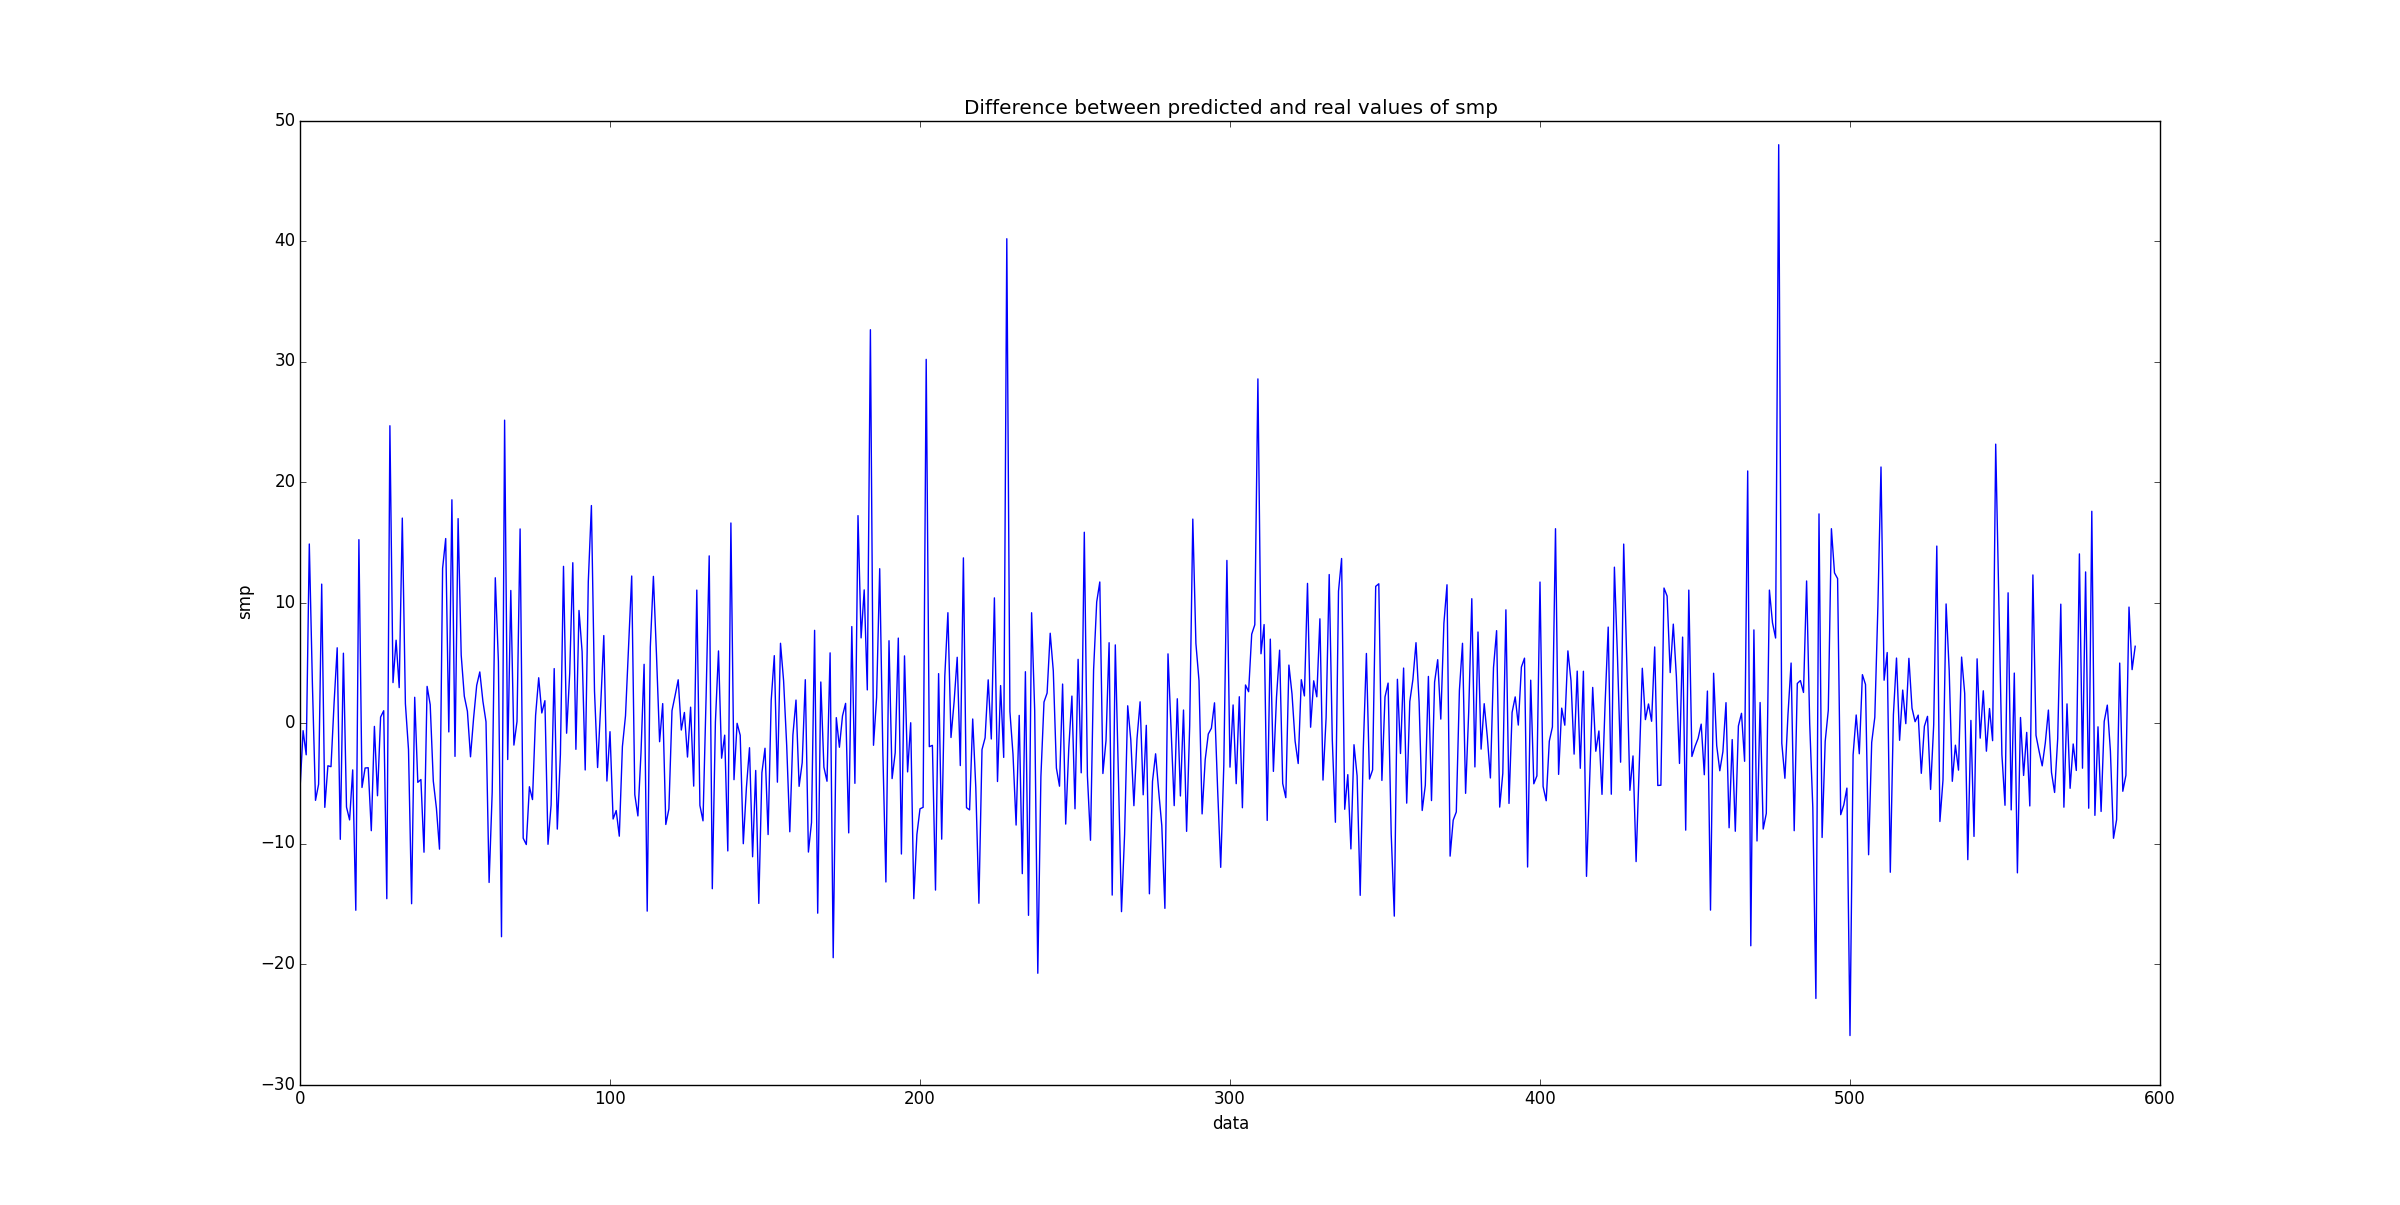
\includegraphics[width=1.3\textwidth]{fig/mars_pred1.png}}%
  \caption{\tl{MARS}: ����������� ��� ������������ ����� ��� \tl{SMP}}
  \label{figure:26}
\end{figure}

\begin{figure}
  \makebox[\textwidth][c]{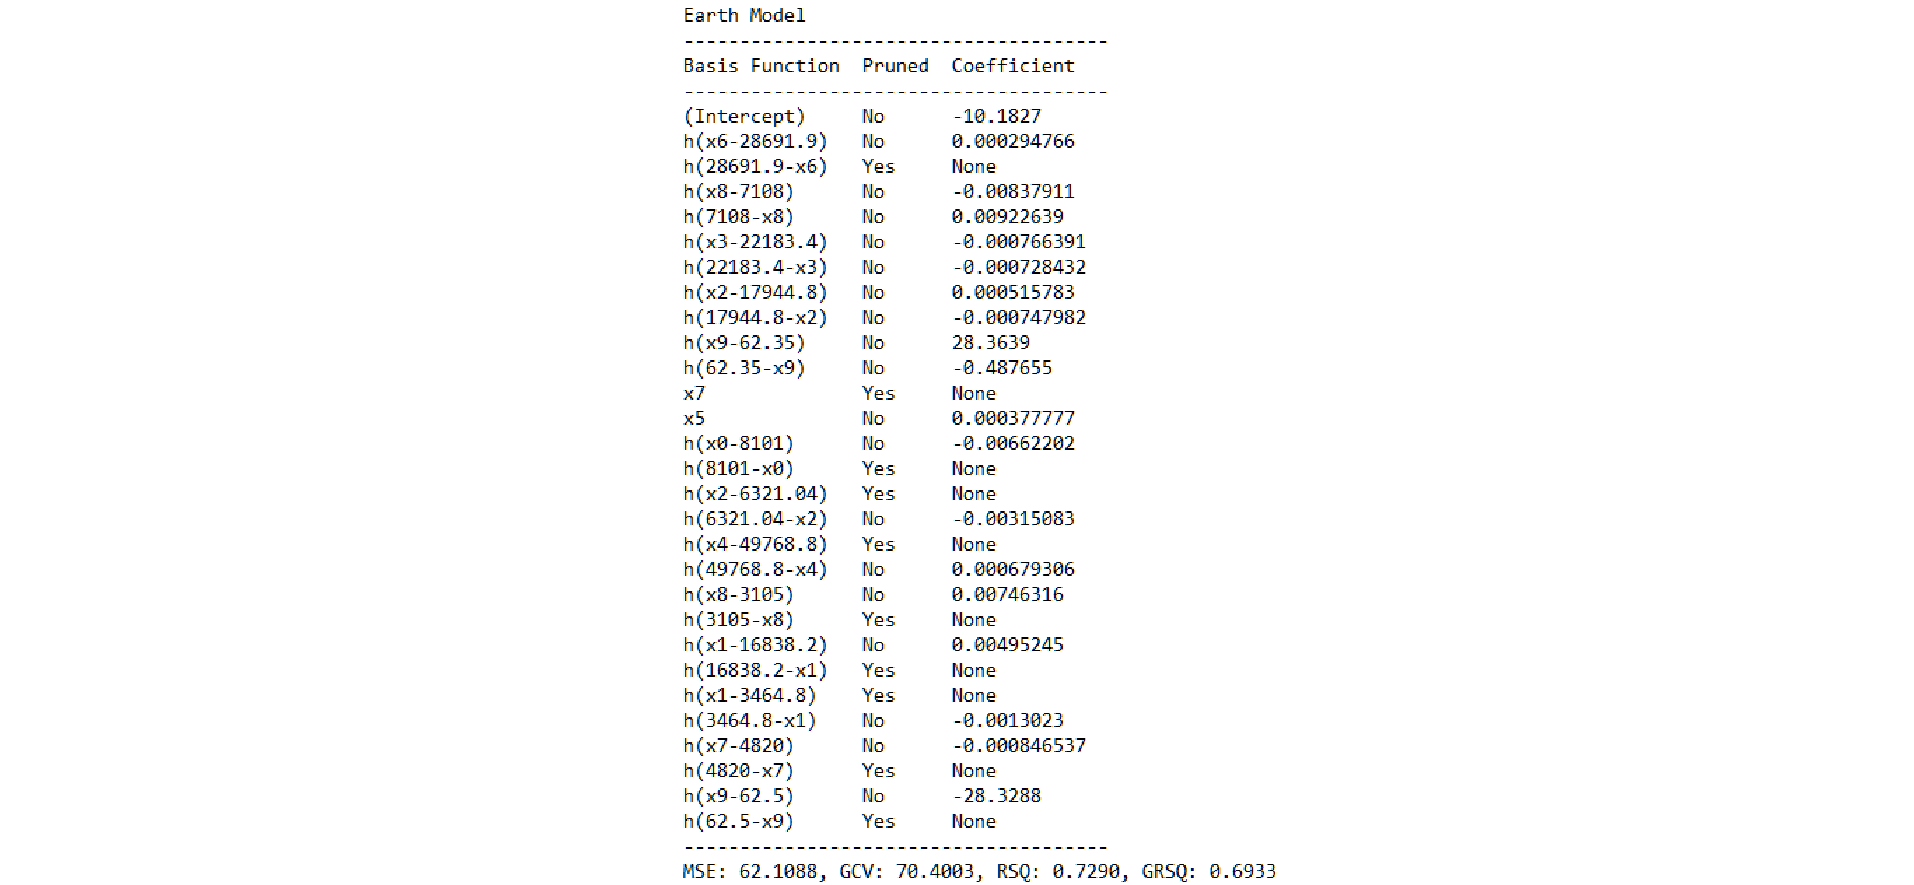
\includegraphics[width=2.3\textwidth]{fig/earth.png}}%
  \caption{\tl{MARS: Earth Model}}
  \label{figure:25}
\end{figure}


%\newpage
%\section{�������� ���������}
%
%������ ��������� ��� ����� \tl{SMP-ngas} �� ��� ��������� ��� ������������ �� \tl{trendline} (�� ����� ������������ ��� ���������). ������ ��� ��� ����� ���� ������������ �� ���������� ��������.
%
%\begin{figure}
%  \makebox[\textwidth][c]{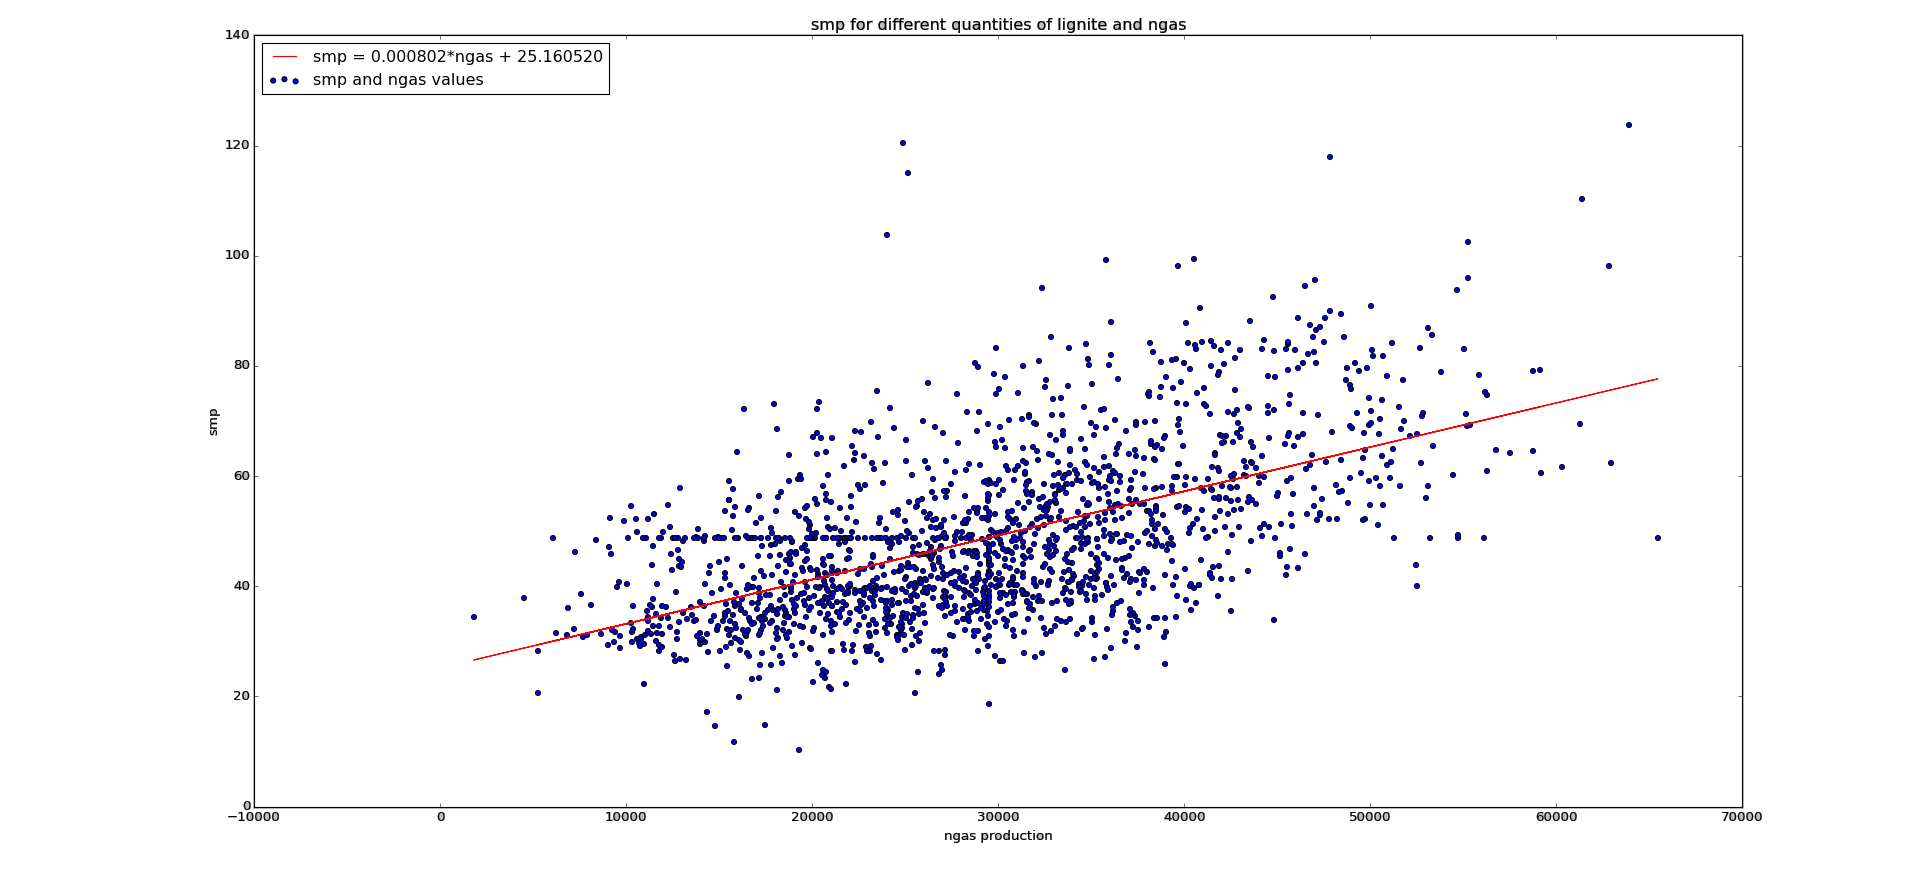
\includegraphics[width=1.4\textwidth]{fig/smp-ngas.png}}%
%  \caption{\tl{SMP and ngas}}
%  \label{figure:27}
%\end{figure}
%
%\begin{minted}[linenos]{python}
%smp = train_imp[:,0]
%ngas = dataset[:,6]
%plt.scatter(ngas,smp, label = 'smp and ngas values')
%z = np.polyfit(ngas, smp, 1)
%p = np.poly1d(z)
%plt.plot(ngas,p(ngas),'r', label='smp = 0.000802*ngas + 25.160520')
%plt.ylabel('smp')
%plt.xlabel('ngas production')
%plt.title('smp for different quantities of lignite and ngas')
%plt.legend(loc='upper left')
%plt.show()
%print 'smp = %.6f*ngas + %.6f'%(z[0],z[1])
%\end{minted}
%
%����������� ��� ���� ��� �������� ��������� ������ ��� ��� ��������� ������ ������� 30\% ��� �������� ��� ����� �� ���� ������� ������ �� 9.6\euro. \\
%
%�������� ��� ���� ���������� �� ����� ���������� ����������� ����� ����� � ����������� ��� �� \tl{importance score} ��� \tl{random forest} ��� \tl{CART}. ����������� ������ ��� �������� ���� ������������ ���� �� ���������� \tl{ngas}, \tl{waters} ��� \tl{load\_forecast} �� ��� ���������� �� ����� ������� ��� 15\%. �� ��������� ��� ��� �� ������� ���� ����� ���� �������� ��������� ��� ��������� �� ����� �� �� \tl{SMP} ��� �� ����� ��������� ��� ������ �� �������������� ��� �������� ��� ����� ���� ��� �������� ������ ��� ���������������. ����� ���� ���������� �� ������� ��� � ���� ��������� ����������� �������� ����������� �� ���� �� ���� ���� ������ �� ��������� ��� ����� �� ����� �� ���� ����������� ��� ���������� ����.

%\begin{figure}
%  \makebox[\textwidth][c]{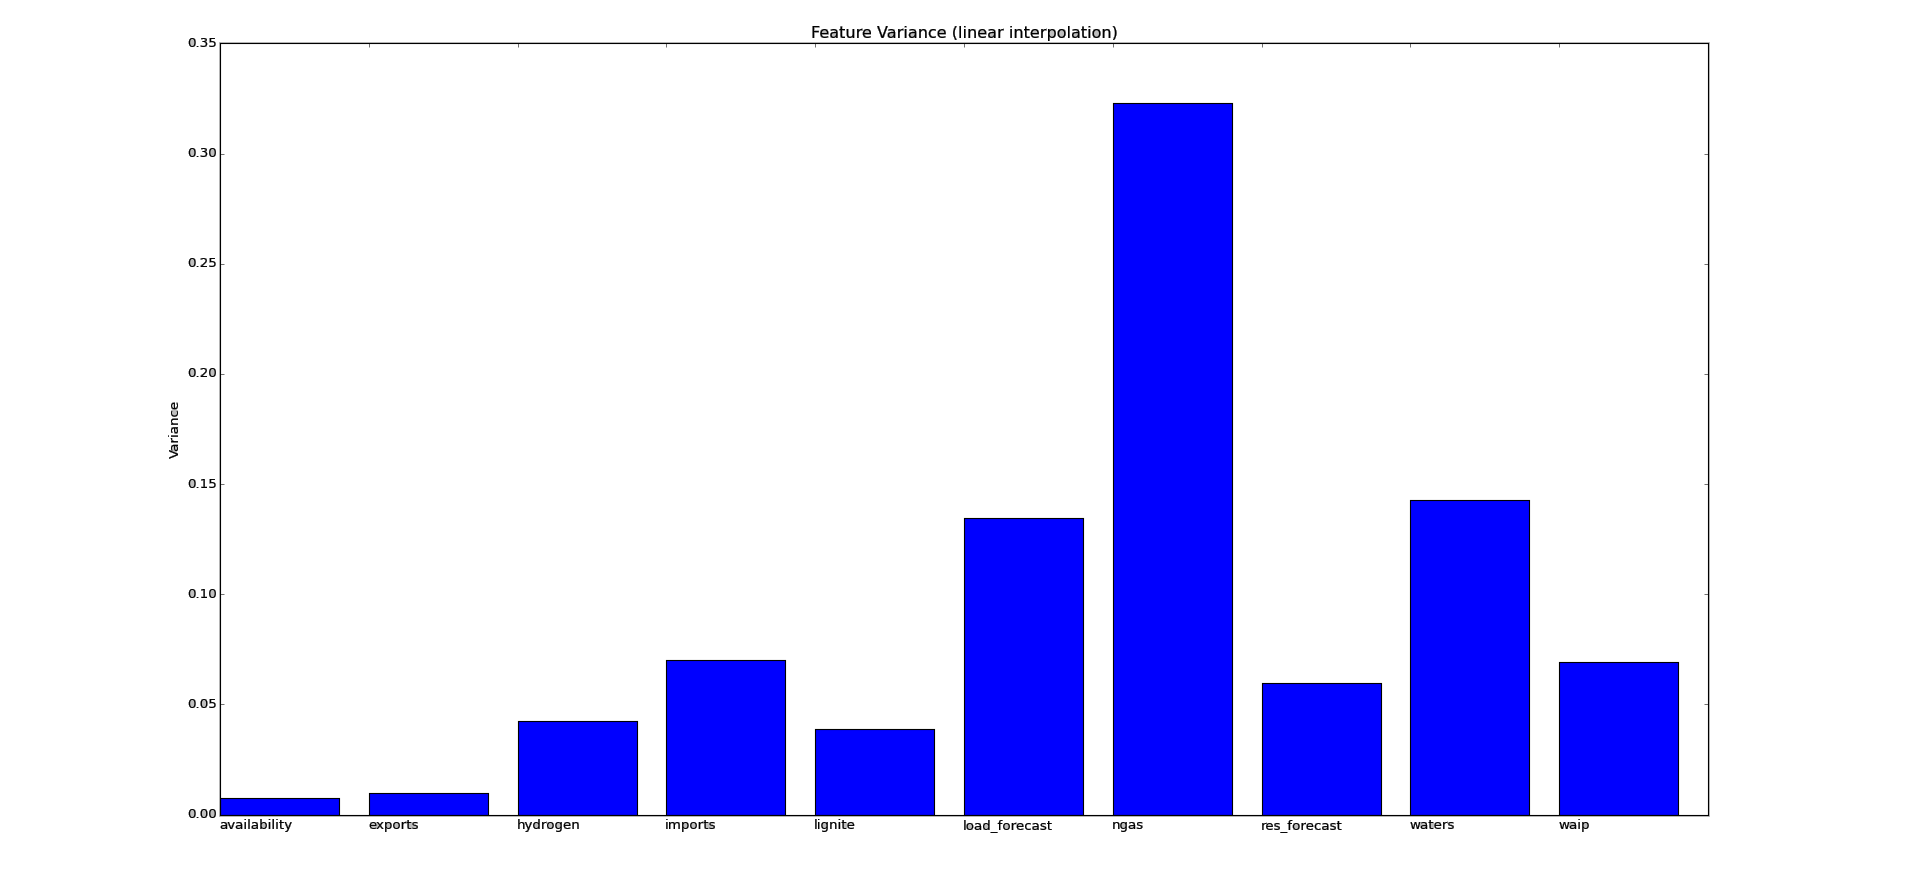
\includegraphics[width=1.4\textwidth]{fig/variance_inter.png}}%
%  \caption{\tl{Feature Variance - Linear interpolation}}
%  \label{figure:28}
%\end{figure}
%
%
%��� ����� \ref{figure:29} ������ ��� \tl{scatterplot} ��� \tl{SMP} �� ��������� �� ��� ���������� \tl{ngas} ��� \tl{waters} �� ������ ���� �� ��� ���������� ���� ������� ���. ����������� ��� �������� ������ ��� ����� ��� ��� ��������������� ��� ��� \tl{SMP}.
%
%
%\begin{figure}
%  \makebox[\textwidth][c]{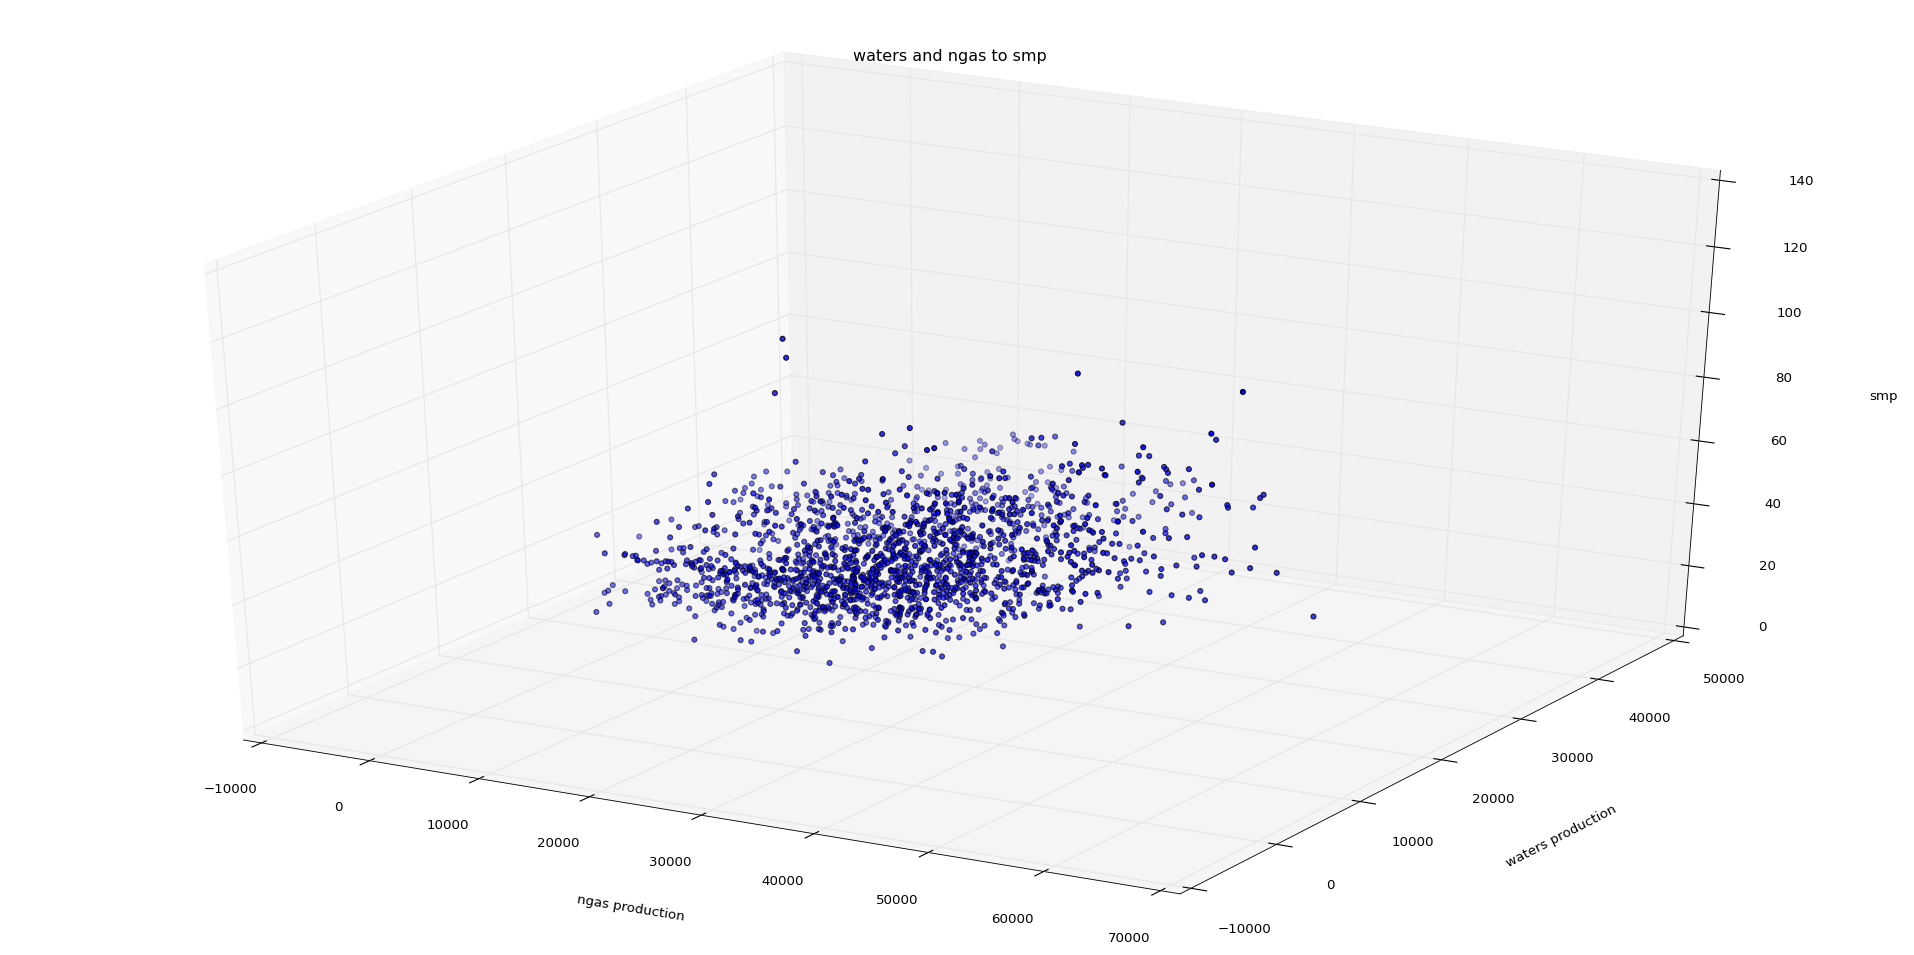
\includegraphics[width=1.4\textwidth]{fig/ngas_waters.png}}%
%  \caption{\tl{Waters and ngas to SMP}}
%  \label{figure:29}
%\end{figure}


\newpage
\thispagestyle{empty}
\chapter{������� �����������}

\section{��������}

���� ����������� ������� ������ ��� ��������������� �� ���������� ���� �� �������� ��� ���������� ����������� ������ �������� ��������� ��� \tl{training} ��� \tl{validation sets} ��� ������������ ���� ����������� ��� ��� ����������� ���� ���������. �� ���� �� �������� �� ����������� �� \tl{predictions} ���� ���� ����� ����� �� ���������� �������� �� ������ ��� ���������. � ���������� ���� ����� ������ ����������� ����� ������ ��� \tl{test set} �� ��������������� ������� ����� ���� ������������������� ���������� ��� �������� ��� ���������� � ����� �� �������� ������ �� ����� �� �� \tl{training set}, ����� ��� � ���������� ��� ������ �� ��� ����� ���� �������. ������, ������ ��� ���������� �� \tl{trend} ������ �� ����� �� ������ ��������, ����� �������� �������� ��� � ���������� ��� \tl{training set}, ���� ���� ����� �� ��������� �� �������� ������������. �����, ������ ������ ���������� ���� ��������� �� ������� ��' ��� ��� ������������ ����� ��� ���������� ���� �� ����������������� �� �������� ������ ��� �� ����������� ��� ����������� ��������� ��� �������� ���.

\section{\tl{Residuals} ��� \tl{lagged values}}

��� ���������� ��� ������������ ������ ��� ������� ����������� ��� ����� �������� ��� ��� ����������� ���� ���� ��� ��� ��� ������ ������� ��� ���� \tl{linear regression} ��� ������������ ��� ��������� ��� ������ $y = \alpha x + \beta$. ������ ���� ��� ���������� ��������� ��� ����������� ������������� �����. �� \tl{residuals} ����� �� �������� ��� ���������� ��� ��� ����������� ��� ��� ������������� �����. � ������� ��� \tl{residuals} ��� ��� ��������� ����� ���� ����������� ����� ��� ����������: ���� ����� ��������� ��������� ��� ����������� ���� ��� ��� ������ ���������� ��� ���� ������� ��������� ��� ��� ������� ����������. \\

\begin{figure}
  \makebox[\textwidth][c]{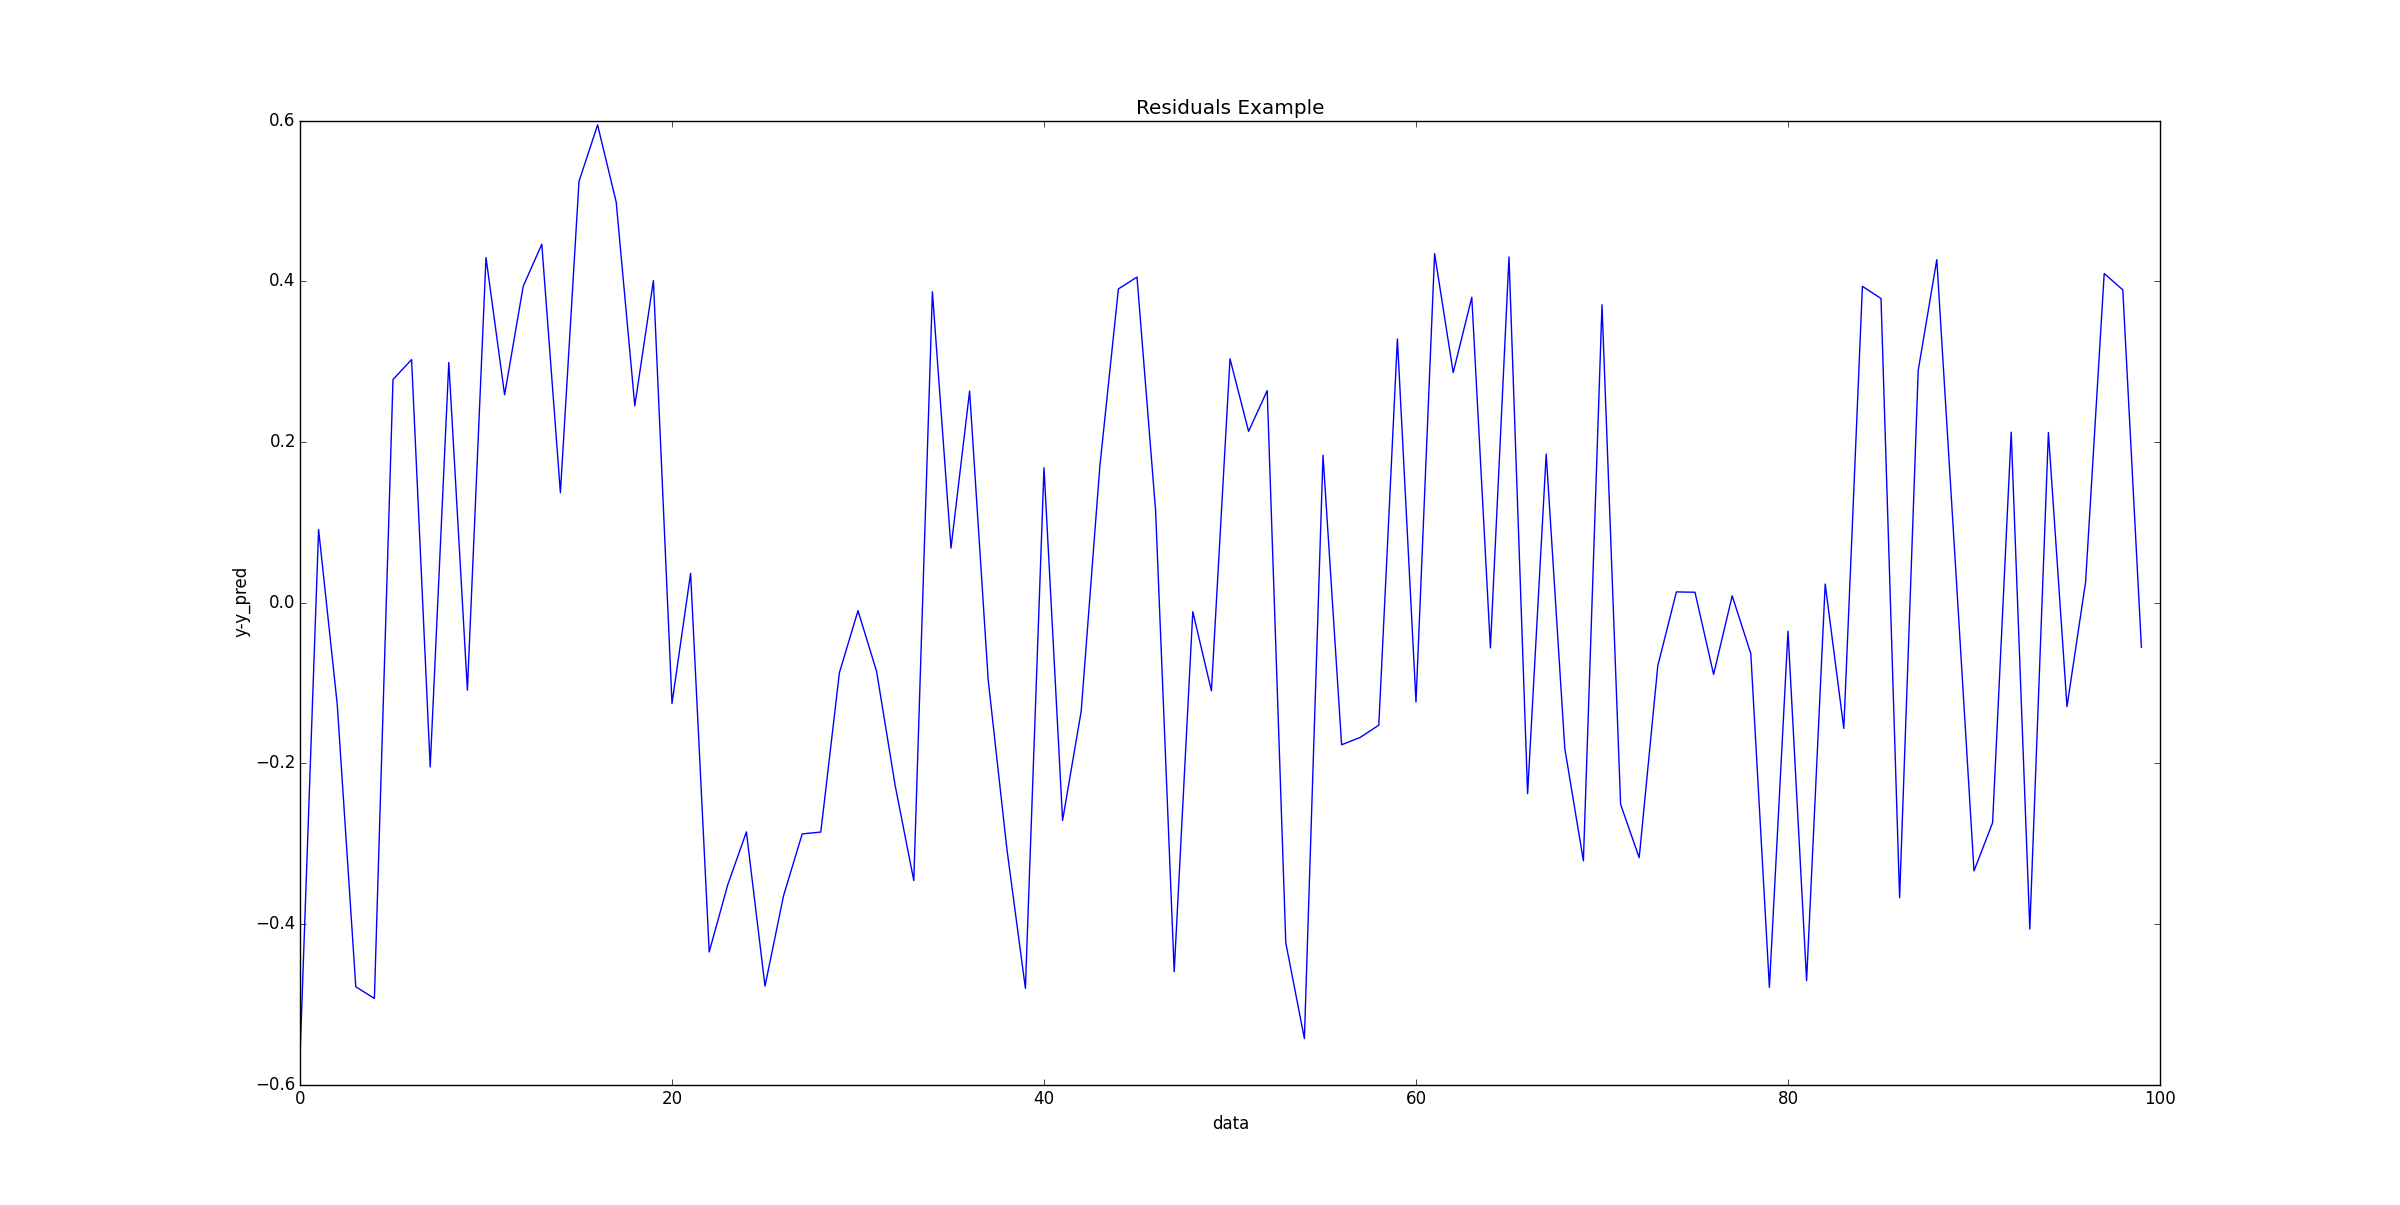
\includegraphics[width=1.3\textwidth]{fig/residuals.png}}%
  \caption{\tl{Residuals Example}}
  \label{figure:50}
\end{figure}

\begin{figure}
  \makebox[\textwidth][c]{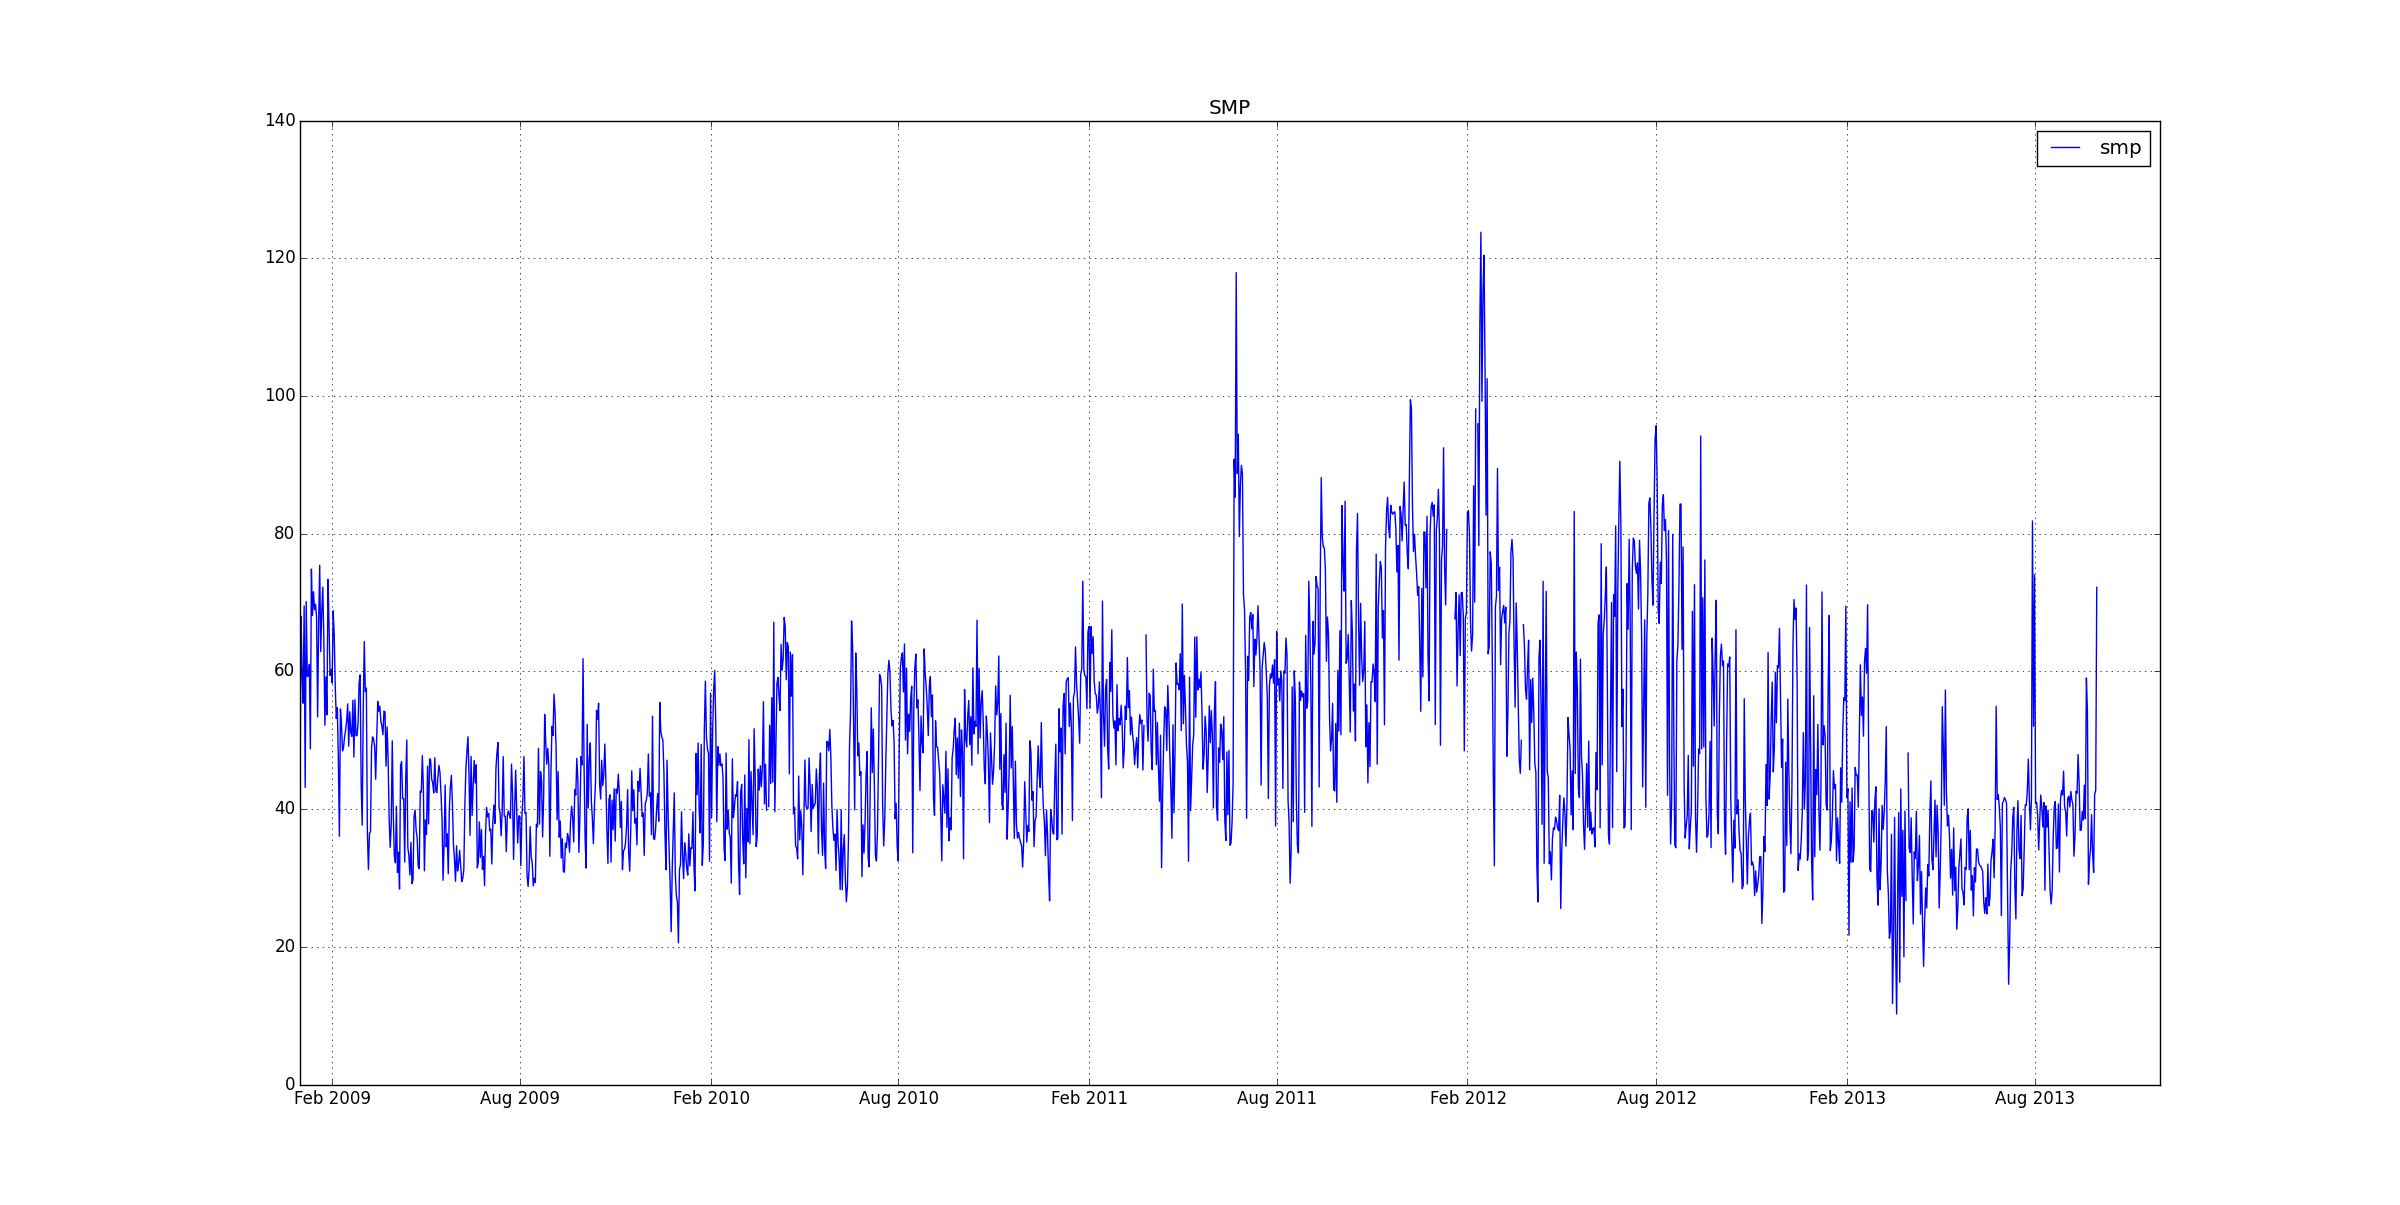
\includegraphics[width=1.3\textwidth]{fig/smp.png}}%
  \caption{���������� \tl{SMP}}
  \label{figure:51}
\end{figure}

�� ��������� ������� �� �� \tl{residuals} ����� ��� ������� ��� ������� ��� ������������ �� \tl{residuals} �� ������� ��� �����. ������� ���� ������� ��������� � ����� ���� ����� ����� ��� �����. ��� ���������� ������ ��� �������� �����������:

\begin{equation}
X(t) = X(t-1) + \varepsilon (t), X(0)=0, \varepsilon\sim N(0,1)
\end{equation}
\begin{equation}
Y(t) = 0,2*Y(t-1) + z (t), Y(0)=0, z\sim N(0,1)
\end{equation}

��� ����� \ref{figure:50} ��������� �� \tl{residuals} ��� �������������. ����������� ��� �� ����� ��� ��������� ����������� ����� ��� �����. ������� � ����� ���� ��� \tl{residuals} ��� ������������ ���������� ����� 0.0028.

\begin{minted}[linenos]{python}
import numpy as np
import matplotlib.pyplot as plt
n=100
e = np.random.rand(n) 
x =np.zeros(n)
for i in range (1,n):
    x[i] = x[i-1] + e[i-1]
    
z = np.random.rand(n)
y =np.zeros(n)
for i in range (1,n):
    y[i] = 0.2*y[i-1] + z[i-1]
    
reg = np.polyfit(x, y, 1)
y_pred = reg[0]*x + reg[1]
res = y-y_pred

m = 0
for i in range(1,n):
    m = m + res[i-1]
ave_res = m/n

plt.figure()
plt.plot(res)
plt.xlabel('data')
plt.ylabel('y-y_pred')
plt.title('Residuals Example')
plt.show()
\end{minted} 
\newpage
�� ��� �������� \tl{lagged} ����������, ������ ���������� ��� ��������� ��� ������������ �������� ����� $t-1, t-2, \dots$, �������� �� ������� �� ������� ��� ��� ������� ��� �� \tl{residuals} ��� ����� ��� �����. �� ���� ��� ����� �� ������ ��� �������� ����������� ���������. ���� ��� ������ �� ����� ������ ���� ���������� ������� ���������� �� ��� �� ������ ��� \tl{training} ��� \tl{validation sets}, ���� ���� ������������ ������������ �����������. ������� �� �� �� �� ������ ��� ����� ���������� � ���, ��������� ��� �� ���������� ������������. ��� ��� ���������� ����� �� ������, ���� ����������� ����� � ����� \tl{lagged} ����������. 

��� ����� \ref{figure:51} ������������� � ���������� ��� \tl{SMP} ��� 1/1/09 ��� 30/11/13. �� ������� ������������� ���� �� ������������ �� ���� ������ �� �������� ��� ����� ��������� ���� �� ����� ��� ������ �� ��������� \tl{training} ��� \tl{validation sets}. ����������� ��� ��� �� ���� ��� 2009 ��� ��� ����� ��� 2011 � ���������� ����� ����� ����� �������� �� ���������� ��� ���� ����� ���������� ��������� ������� �� �������� �� ������� �������������� ����������. ��� �� ���� ��� 2011 ��� ������ ���� � ���������� ��� ����� ����� �������������� ������������ ���� ��� ��������� ��� ����������� ���������� ��� ���������� ���� ���� ���. ������ ��� ��� ������� 2013 ������ ���� ������� ������������ ��� \tl{SMP} ��� � �������� �� ����� ����� �����������. 


\section{������� \tl{lagged} ����������}

������ ���������� ��� ��������� \tl{Random Forests} ��� �������� ��� ��� ����������� \tl{lagged values}. ������������ � ���������� ����������� ��� �������� ����� \tl{lagged} ���������� ��� �������� �� ���������� ������ $t-3$. ��� ��� ���������� ��� \tl{lagged} ���������� ��������������� ��� ������ \tl{shift} ��� ��� ���������� \tl{pandas} ���� �� ������������� �� �������� ���� \tl{dataframe} ��� ������ ��� �������.

� ���������� ����������� ��� ����������� \tl{train} ��� \tl{test sets} ���� ���� ����������, ���������� ��� \tl{training sets} ��� 100 ���������� ��� \tl{training sets} ��� 1600 ����������. �� ������������ ��������� ��� ��������� \ref{figure:52} ��� \ref{figure:55}. ����������� ��� �� ��� �������� \tl{lagged} ���������� �� ������� ����� ��������� ���������� �� ����� �� �� ���������� ����� ��� \tl{lagged} ����������. �� ������� ���� ���� �� ����� �� ��� ������������� ��� �����������, � ����� ��������� �������� ��� �������� ��� �������� ��� ����� ��� ���������� ��������. � �������� ���������� ��� ��������� ���������� ��� ������������ �������� ������� ����� �� ��������� ����� �� ������� ��� ��� �������� ����������. � �������� �������� ����������� ���������� ��������� �������� ������, ������� ���� ��� ��� ������ ��������� �������� ���� �������� ��� ��������. ������� �� �� ��������� � �������� �������� ���������� �� �������� \tl{lagged} ���������� ��� $t-2$. 
\newpage
\begin{figure}
  \makebox[\textwidth][c]{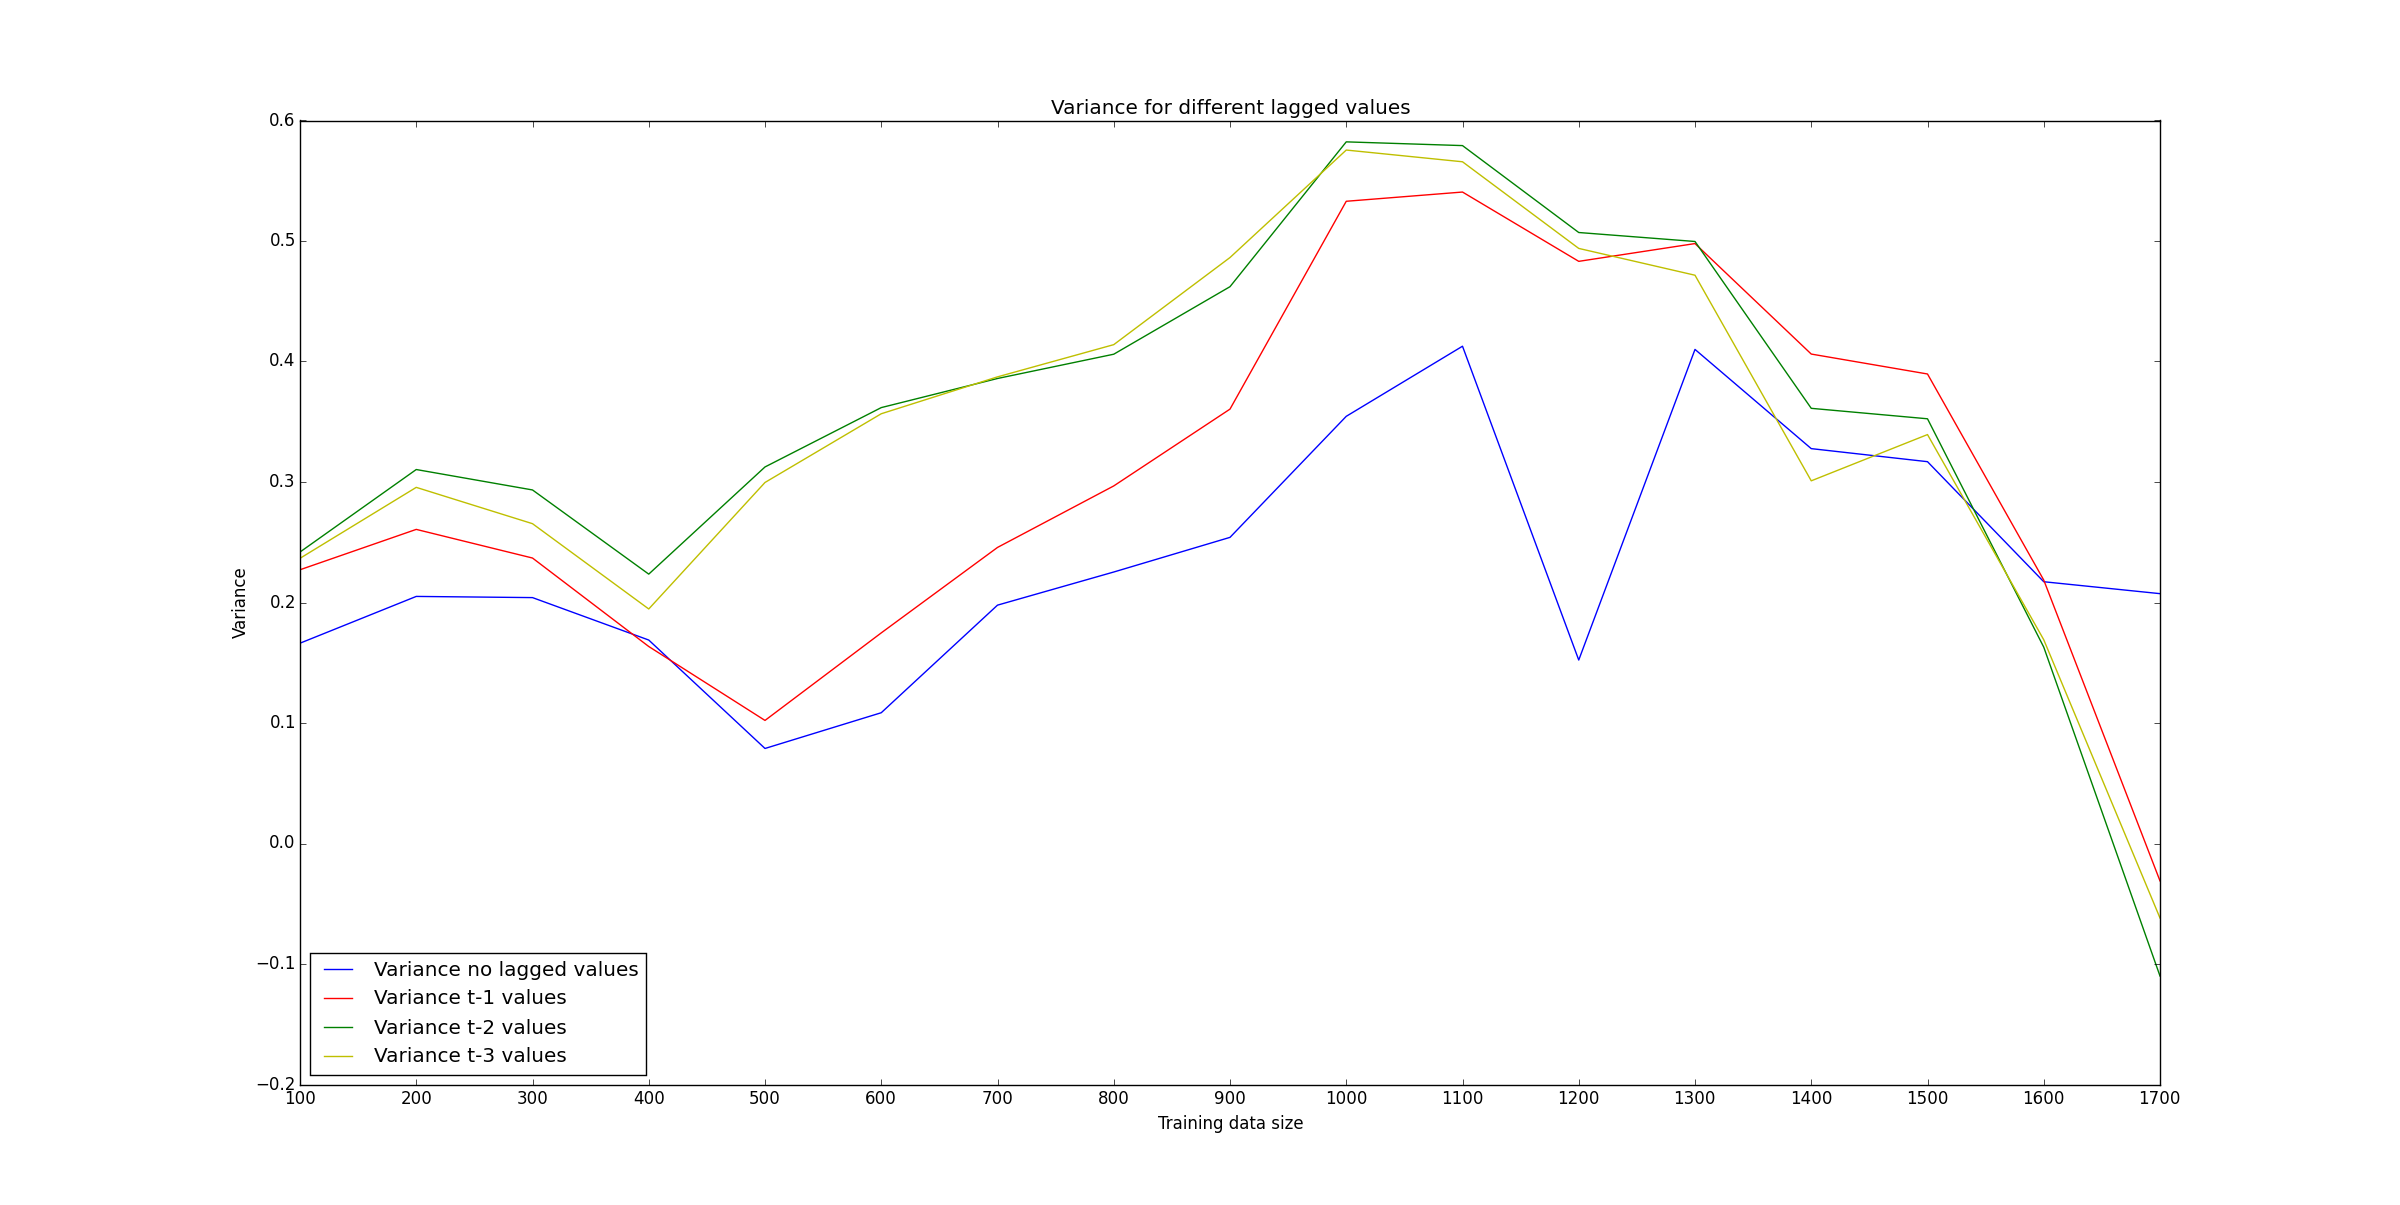
\includegraphics[width=1.3\textwidth]{fig/variance_data_size.png}}%
  \caption{\tl{Variance for different lagged values}}
  \label{figure:52}
\end{figure}
�� ����� ��������� ������ ��� ����������� ����� ��� � �������� ����� ������ ���������� ��� ���� ��� �������� ��� ����������� �������� ���� �������� ��� ���������� �� ������ \tl{training} ��� \tl{validation sets}, ����� ��� �� ��� �������� \tl{lagged} ����������. ���� ����� ���������� ��� �������������� ��� ����������� ��� �������� ���� ��� ��� ������������ ��� ����������� ��� ������������� ��� ����������� ��������. ���� ��� ���������� ��� ������������ ��� ������� ��� ���������� ��������� ���� ������ � �������������� ��� ��������� ��� � �������������� ��� �������� ��� ����������, ����� ��� �� ��������� ��� �������������� ����� ��� ���������� ����. �� ���� ��� ����� ������ ���� �������������� ����� �� ��� ��������� ���� ���� ���������� ���� ��� ��� ������ ��� ���� ���������� ��� ��� ����������� ��� ���������. ���� ������� �� ������ ��� �������� ����� ����������� ��� �������� ���� ��� �� ���� ������ �� ���������� ������������ ��� �������� ����������� �� ����� �� ����������� ����������.   

��� ����� \ref{figure:53} ������ �� \tl{explained Variance} (�������� ��������) ��� �� ����������� \tl{lagged values} ��� ����������������. � �������� �������� ������������� �� \tl{training set} 1000-1100 ����� �� \tl{lagged values}, ������ 60\% ��� ������� ��� 40\% \tl{validation set}. � �������� ����� ����� ��� 60\%, ��� ���� ���� ����������� ��� �� ����������� �������� ���. ������ ����������� ��� ��� ������ \tl{training set}, ����� \tl{test set} ������ ������ ��������, ��� ������� �������� �������� �� �� ������� ����� �� \tl{lagged values}. ���� ��������� ��� ������� ��� �� �������� ��� \tl{SMP} ��� ���������� 3 ����� ������������ ���� ������� ���������� ������ ����.

\begin{figure}
  \makebox[\textwidth][c]{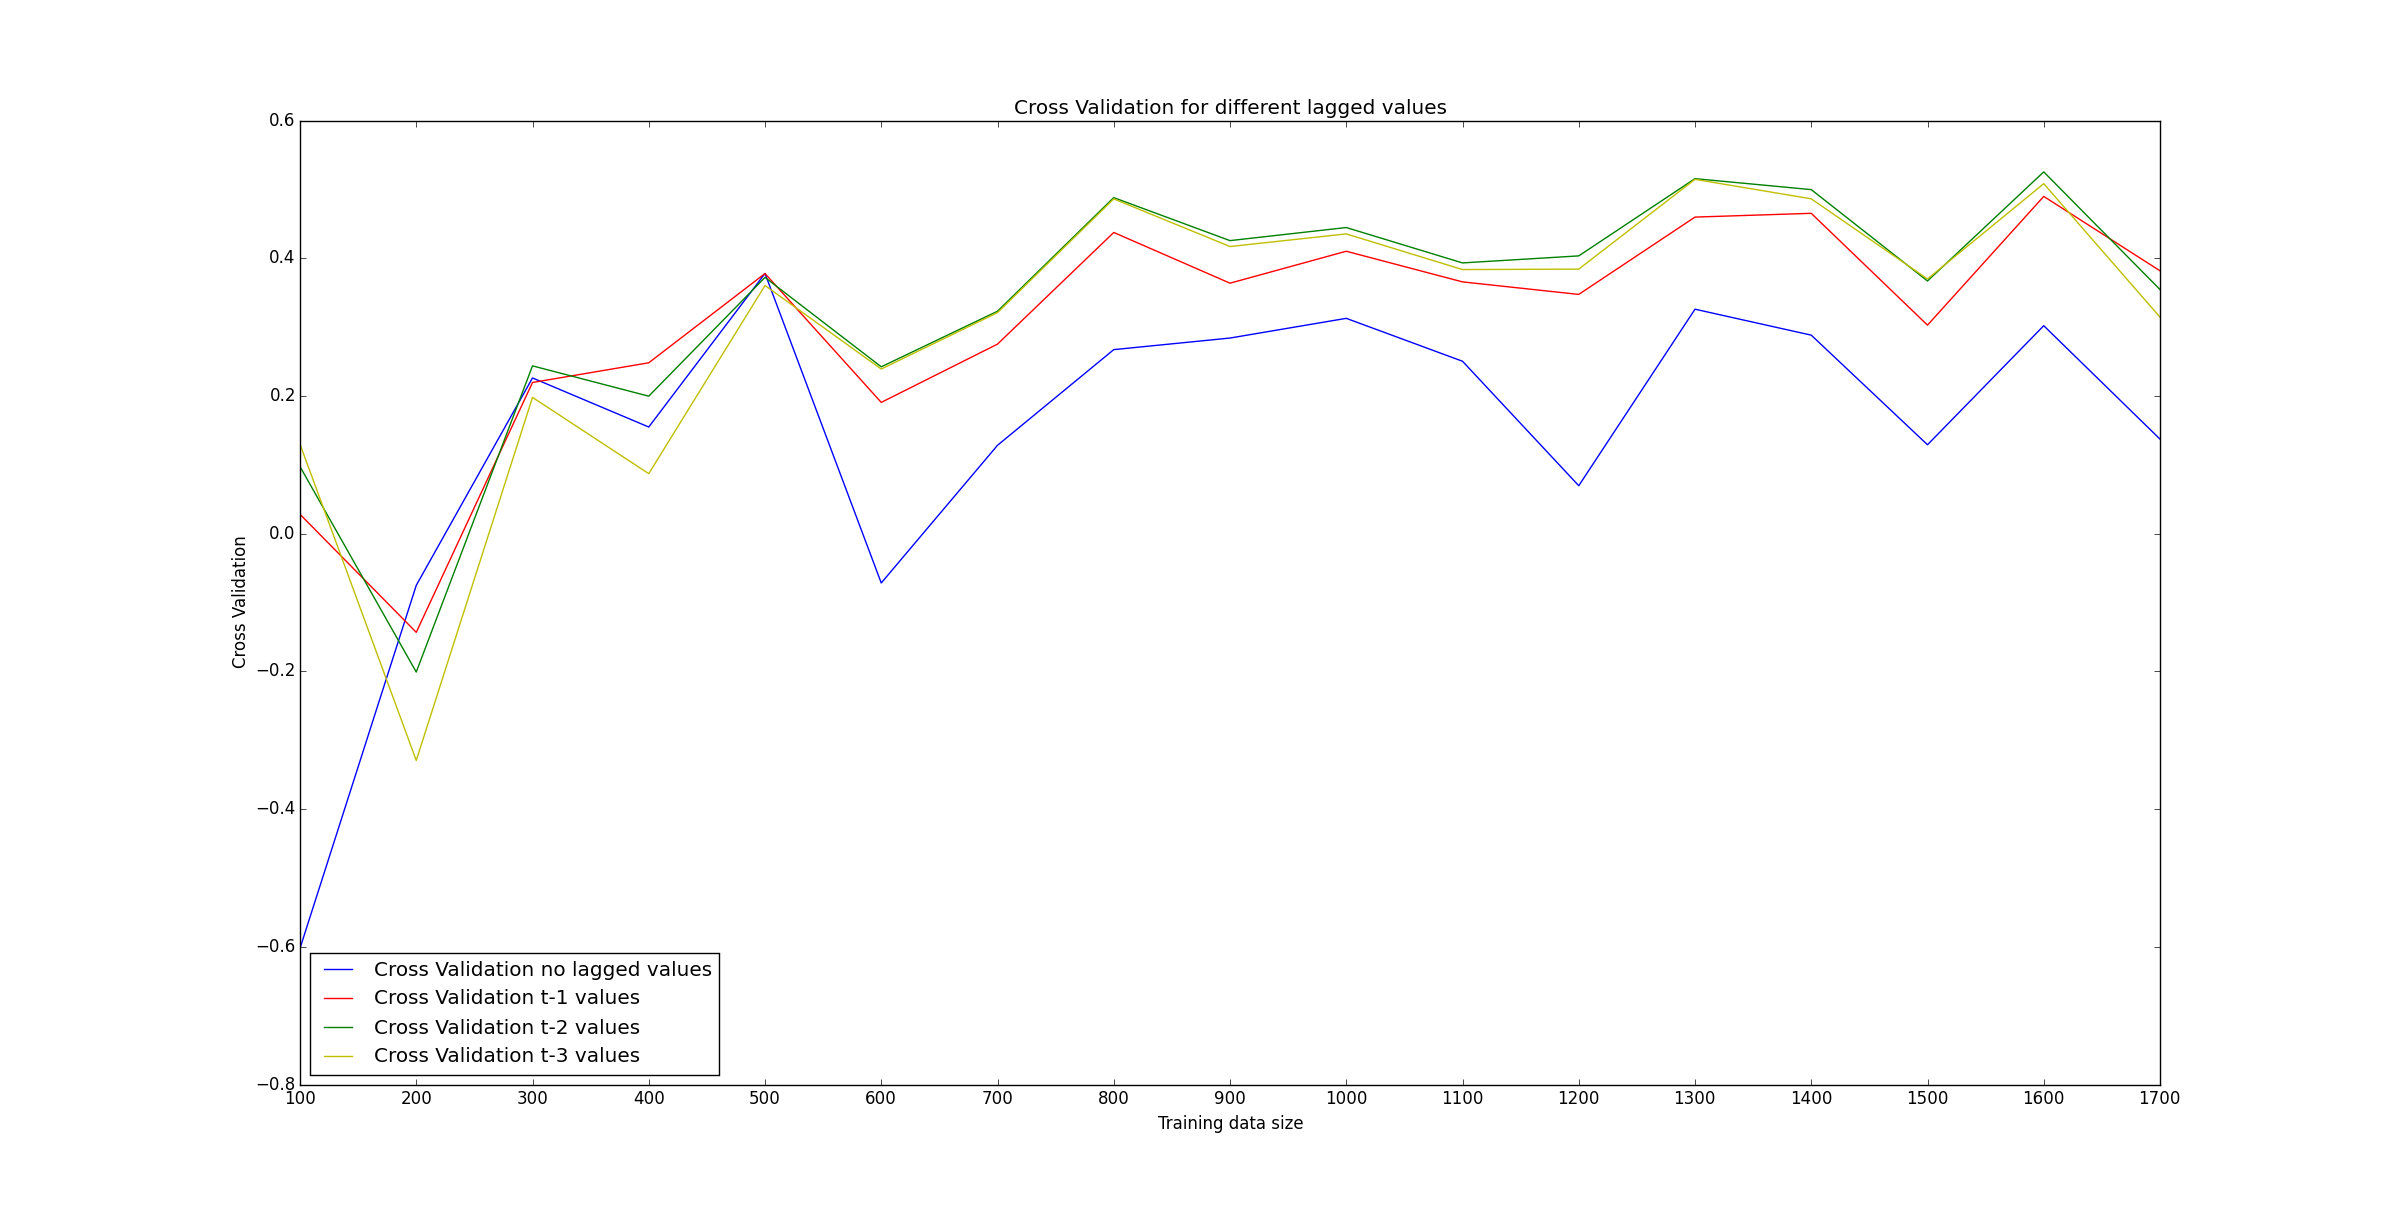
\includegraphics[width=1.3\textwidth]{fig/cross_validation_data_size.png}}%
  \caption{\tl{Cross Validation for different lagged values}}
  \label{figure:53}
\end{figure}

\begin{figure}
  \makebox[\textwidth][c]{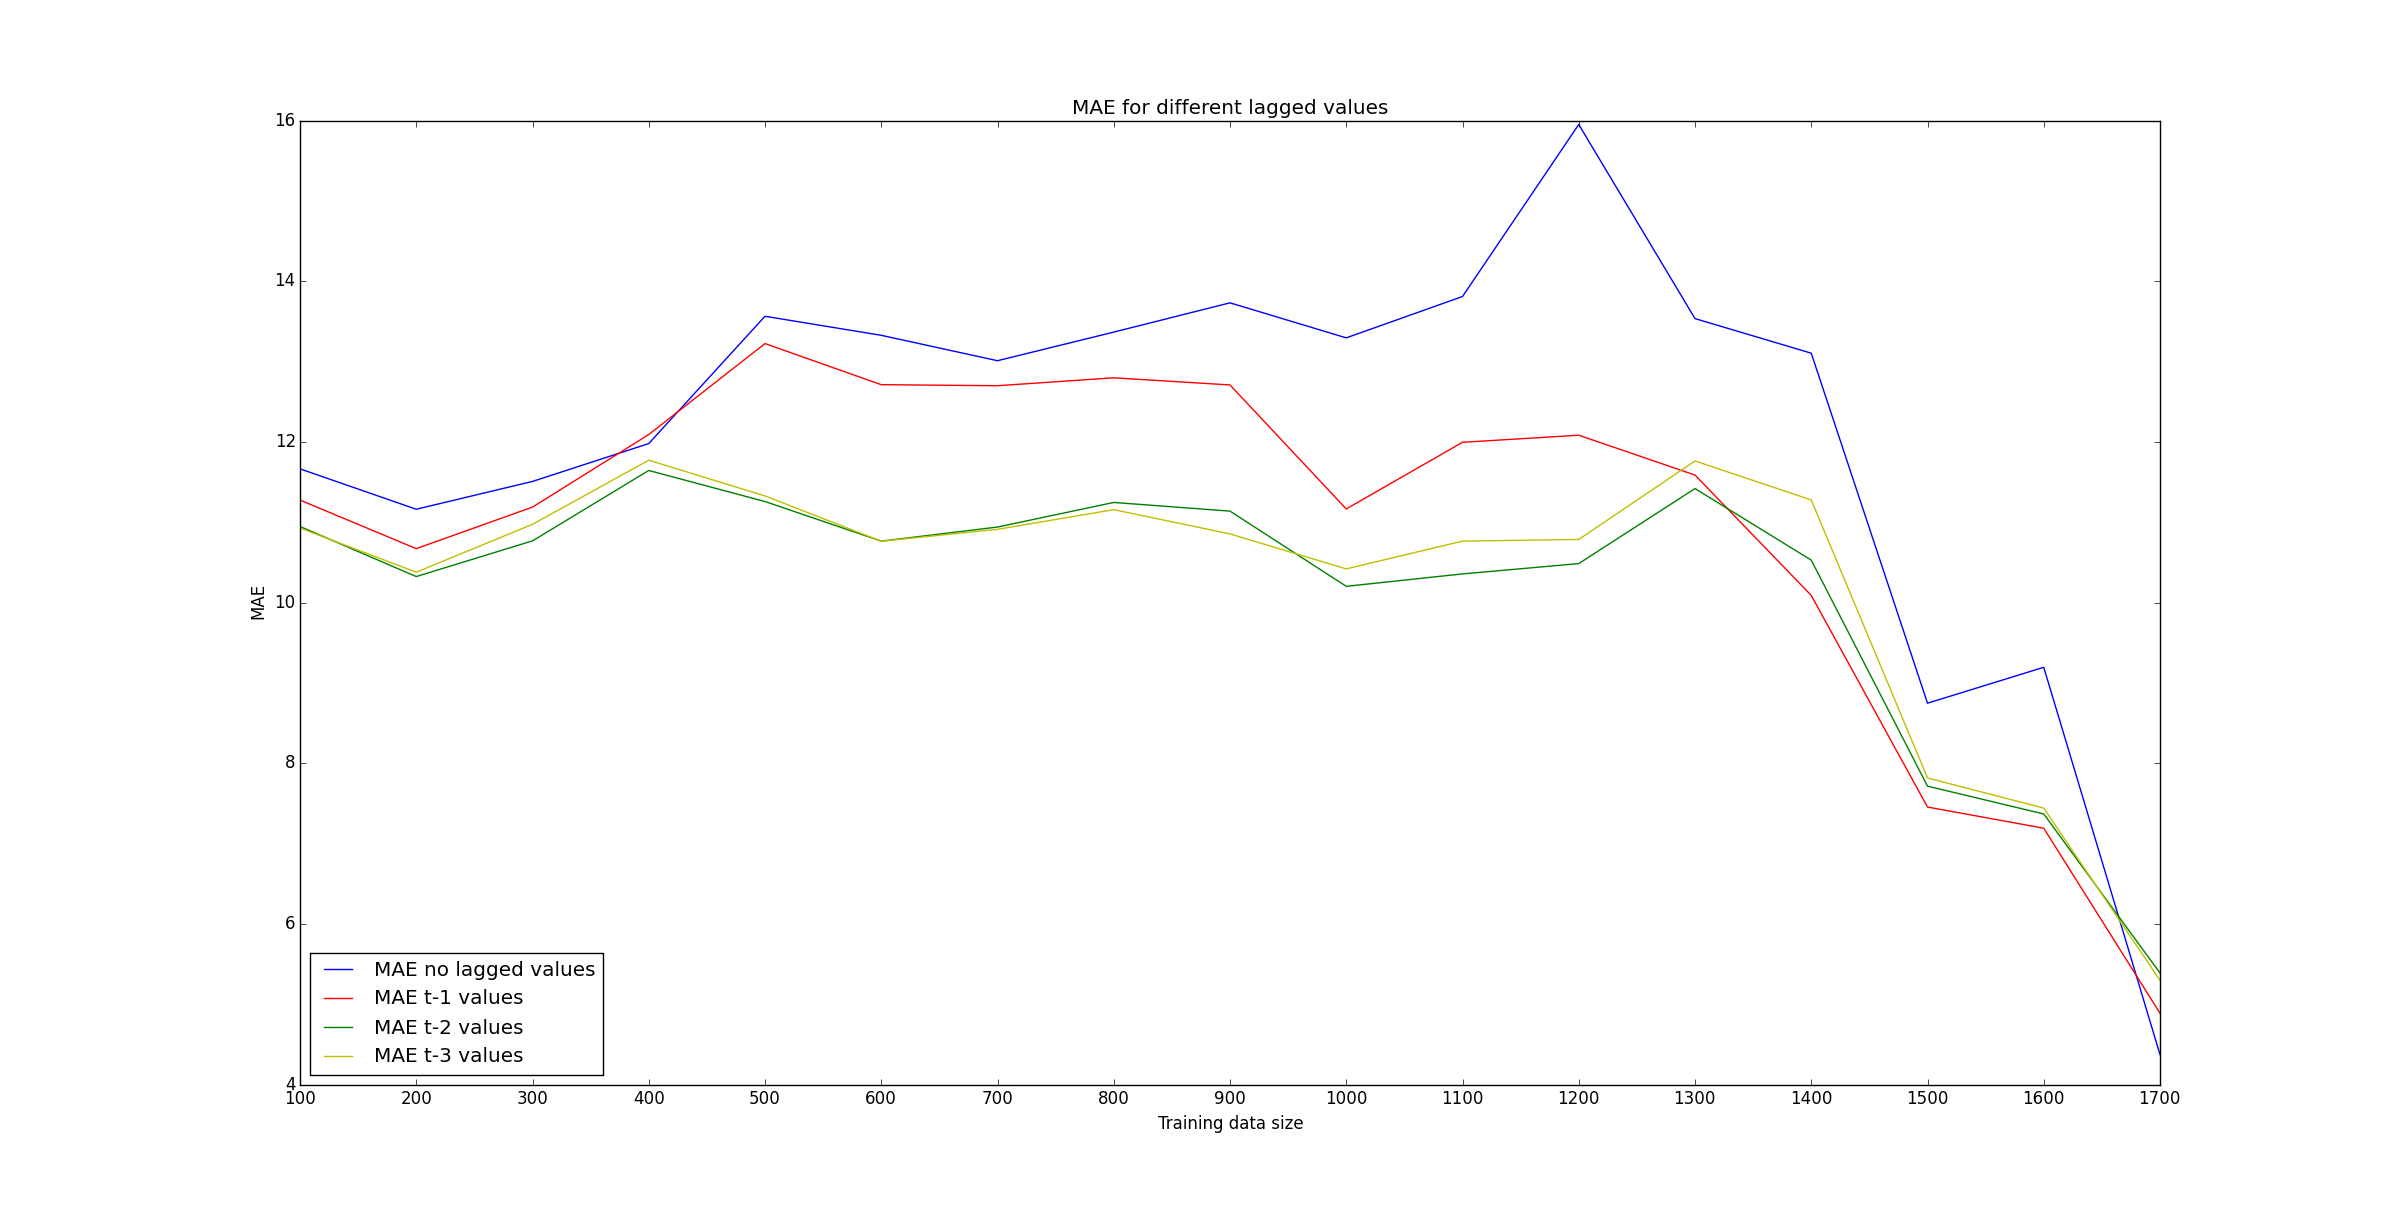
\includegraphics[width=1.3\textwidth]{fig/mae_data_size.png}}%
  \caption{\tl{MAE for different lagged values}}
  \label{figure:54}
\end{figure}

\begin{figure}
  \makebox[\textwidth][c]{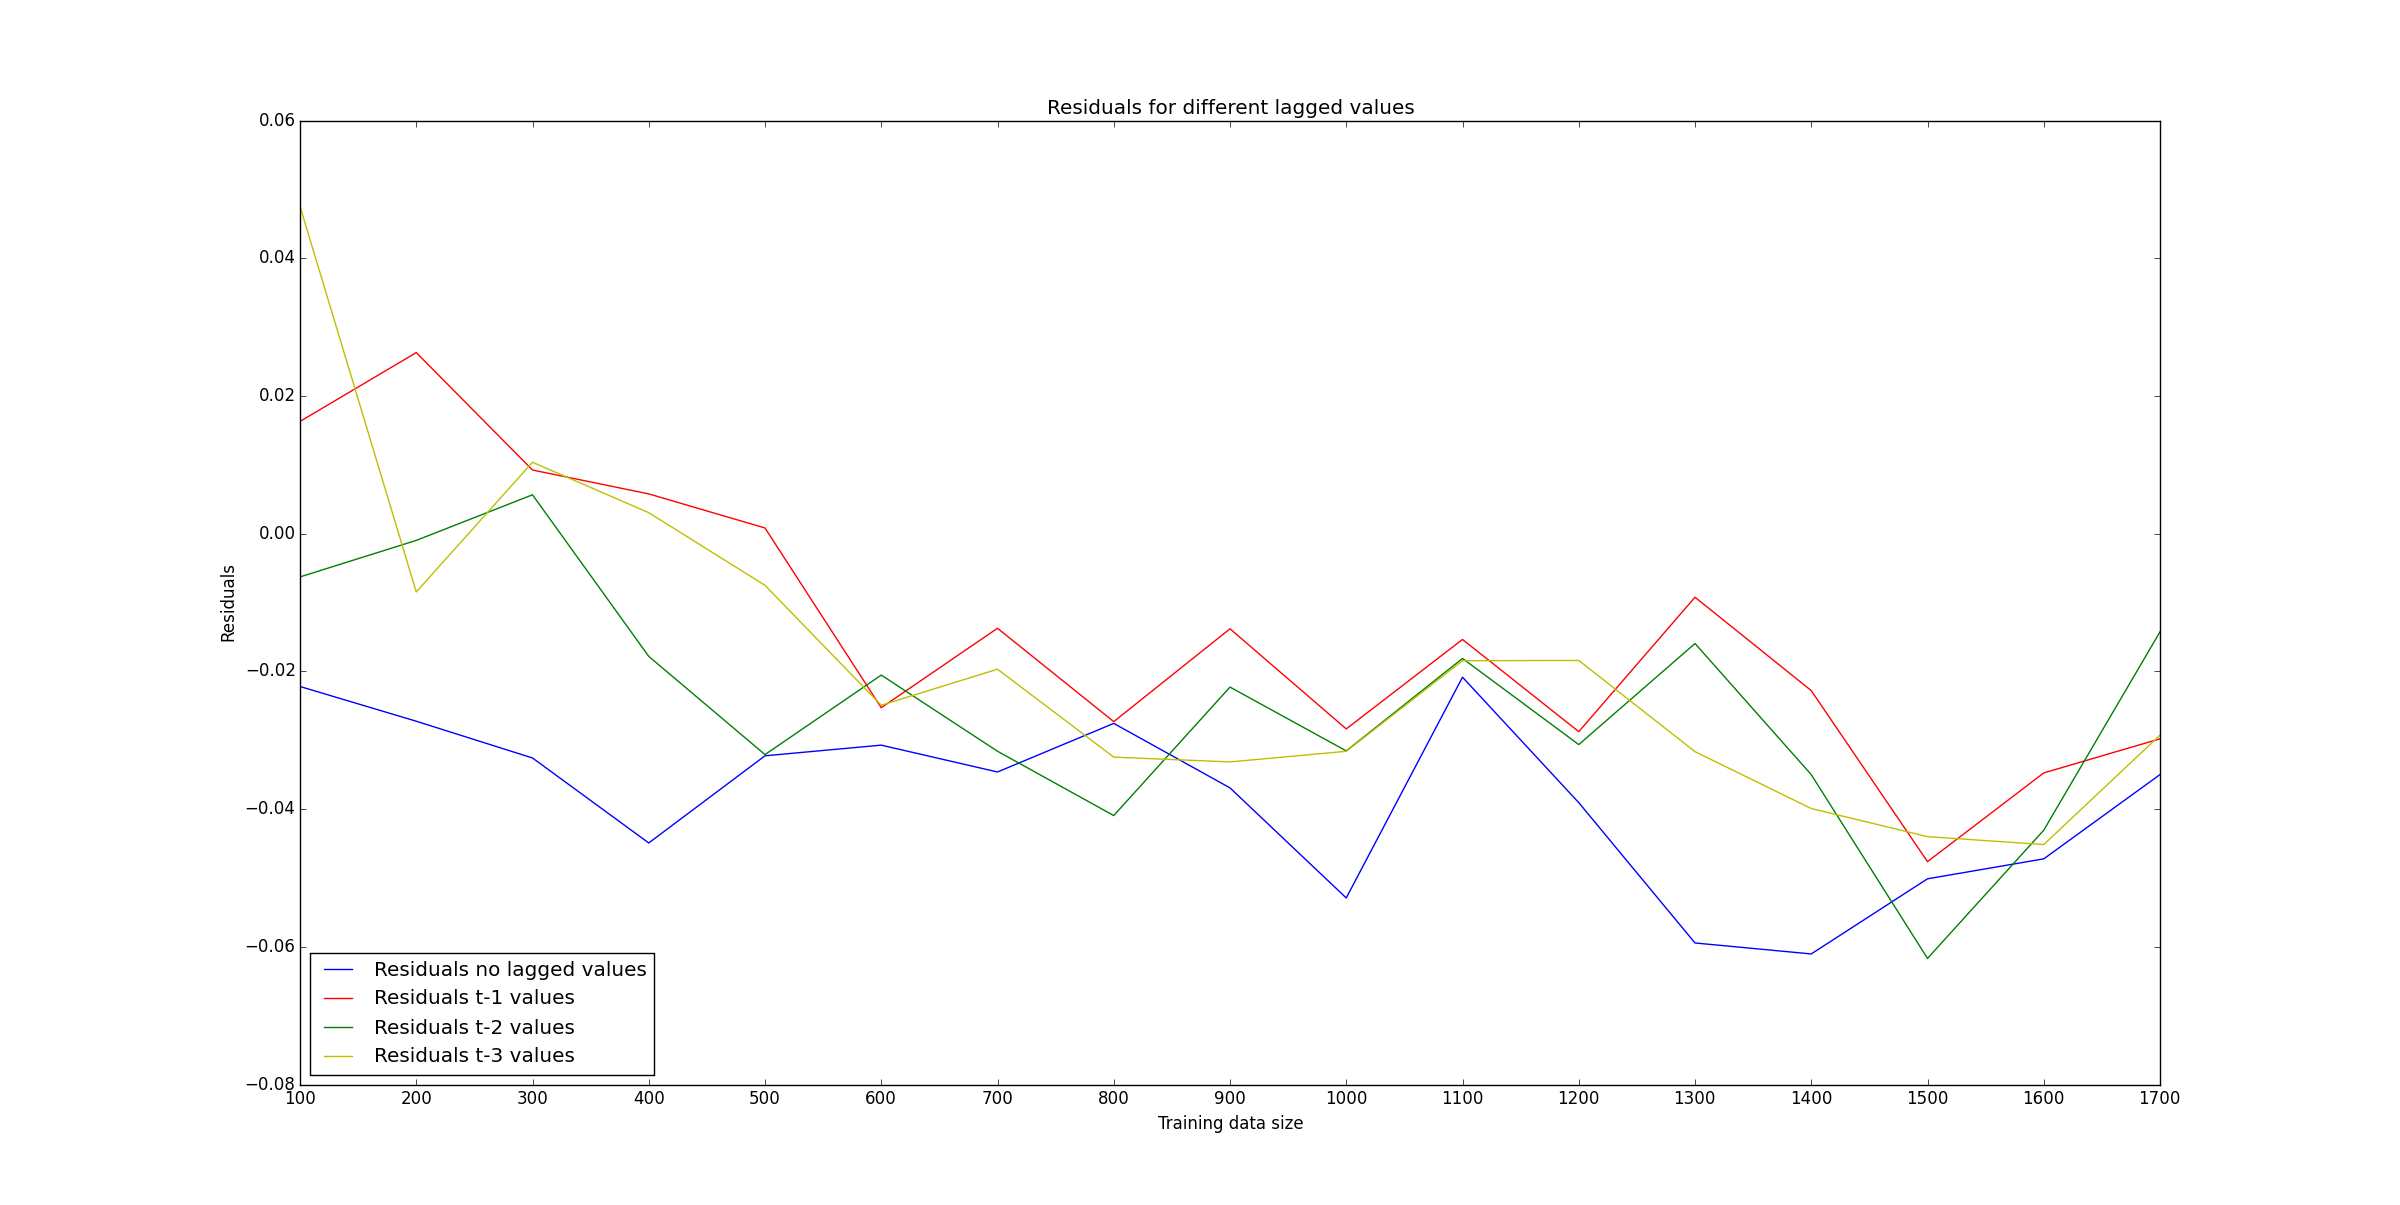
\includegraphics[width=1.3\textwidth]{fig/residuals_data_size.png}}%
  \caption{\tl{Residuals for different lagged values}}
  \label{figure:55}
\end{figure}

��� ������� \ref{figure:53} ��� \ref{figure:54} �������� �� \tl{cross validation} ��� \tl{MAE}. �� \tl{MAE} ���� ��� �� \tl{MSE} ����� �������� ��� \tl{lagged values} $t-2$ ������� ��� �� ���� ��� ������ ����. �� \tl{cross validation} ����� �������� �� \tl{lagged} ����������, ���� ��� ��������� ��� �������� ��� ��� \tl{residuals}. ���� ����� �� \tl{residuals}, ������ ��������� ����� (����� ��� �����) ��� \tl{t-1} ��� \tl{t-2}.

���� ����� �� \tl{importances} ��� ����������, ������� �� �� ������� ��� ��������� ������ ������������ ��������������, �� �� \tl{ngas} �� ���� ��������� ������������� �� ����� �������� ��� �� ������� ������������� ��� ������ ����������� �������� ��� \tl{training set}. ��� ��� ���������� ��� ����� ���� \tl{accuracy} �� \tl{ngas} ���� ������������� ��� 0.34 ����� \tl{lagged values} ��� ��� 0.11 �� \tl{lagged} ���������� ��� ���� � ��� ��������� ��������� ���� � ���� $SMP(t-1)$ �� \tl{importance} ��� 0.45. 

������ ������������ �� ����������� ��� ������������ \tl{test set} �� ����� �������� ��� ���������� 100 ����� ��� �����������, ��� �� ������������ ���� ���������� �� ����. �� ���������� �� \tl{lagged values} ��� $t-2$ ���� �������� ��� �������� ��� \tl{t-1} ��� ��� ������ �� �������� ������������. ��������� �� ������� ��� � ���������� \tl{MARS} ���������� ��� ����� ���� ���� ������������.

��� ������� \ref{figure:56} ��� \ref{figure:58} ��������� �� ���������� ��� \tl{Random Forests} ����� \tl{lagged} ���������� ���� ��� ���������� �� \tl{lagged t-2 values} �� ����� ��� ���������� \tl{Random Forests} ��� \tl{MARS}. � ������� ������ ��� �������� ��� \tl{t-1} ��� \tl{t-2 lagged values} ����� ���� ����� �� ��� ������������� ������������ ��� \tl{t-2}. � �������� ������� �� ����� �� \tl{lag t-2} ����� ����������� \tl{Random Forest}, \tl{MARS} ��� \tl{CART}. 

\begin{figure}
  \makebox[\textwidth][c]{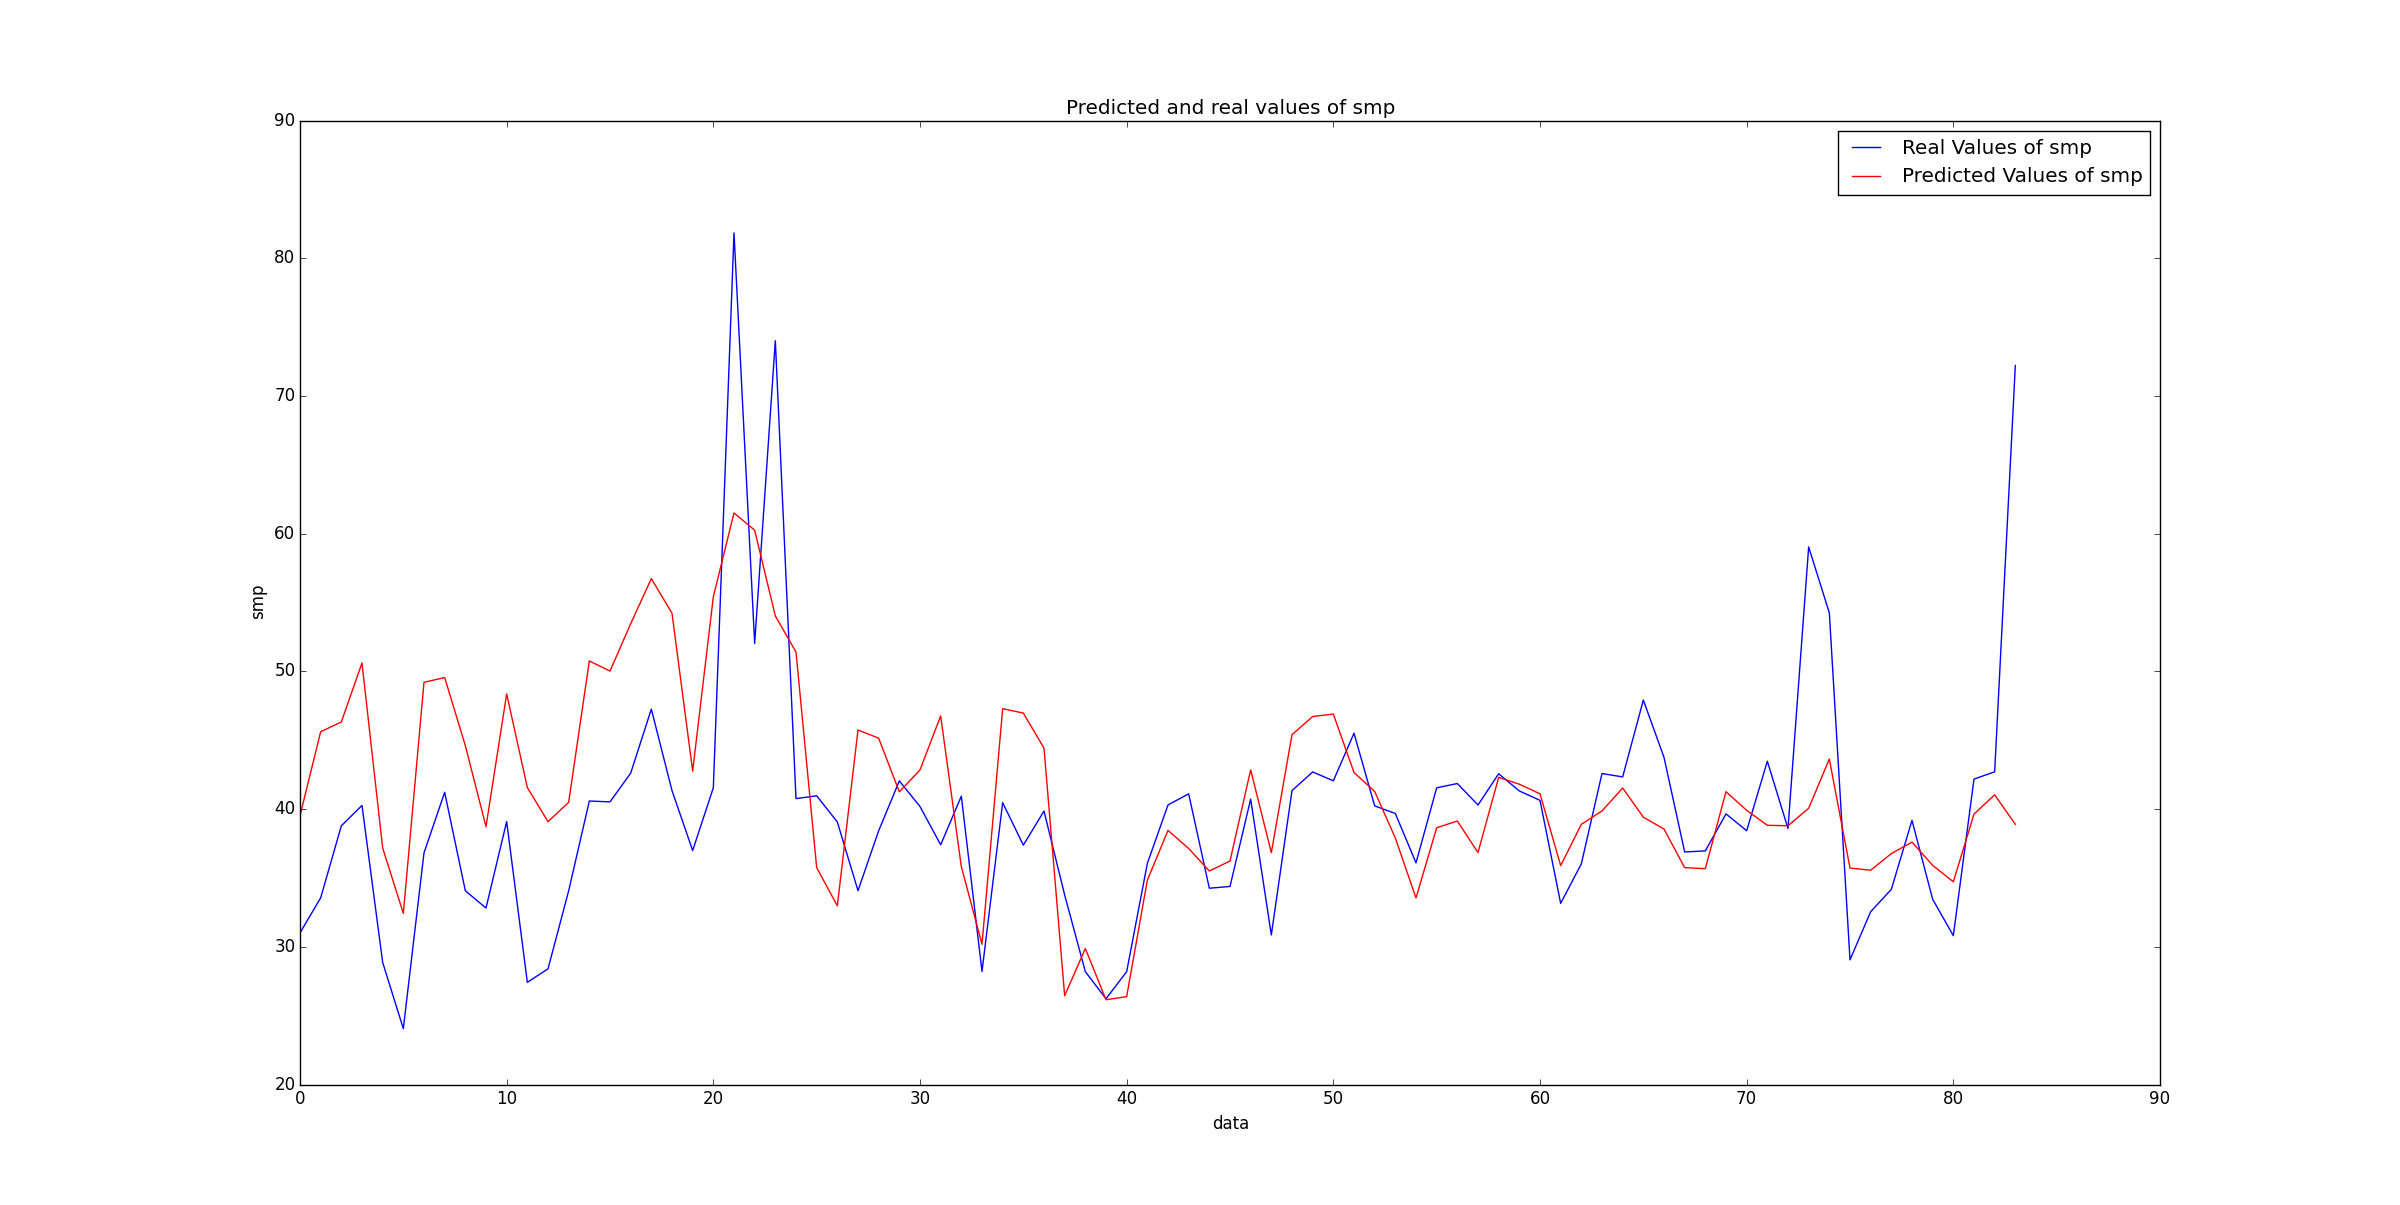
\includegraphics[width=1.3\textwidth]{fig/no_lagg.png}}%
  \caption{\tl{Random Forest - no lag}}
  \label{figure:56}
\end{figure}

\begin{figure}
  \makebox[\textwidth][c]{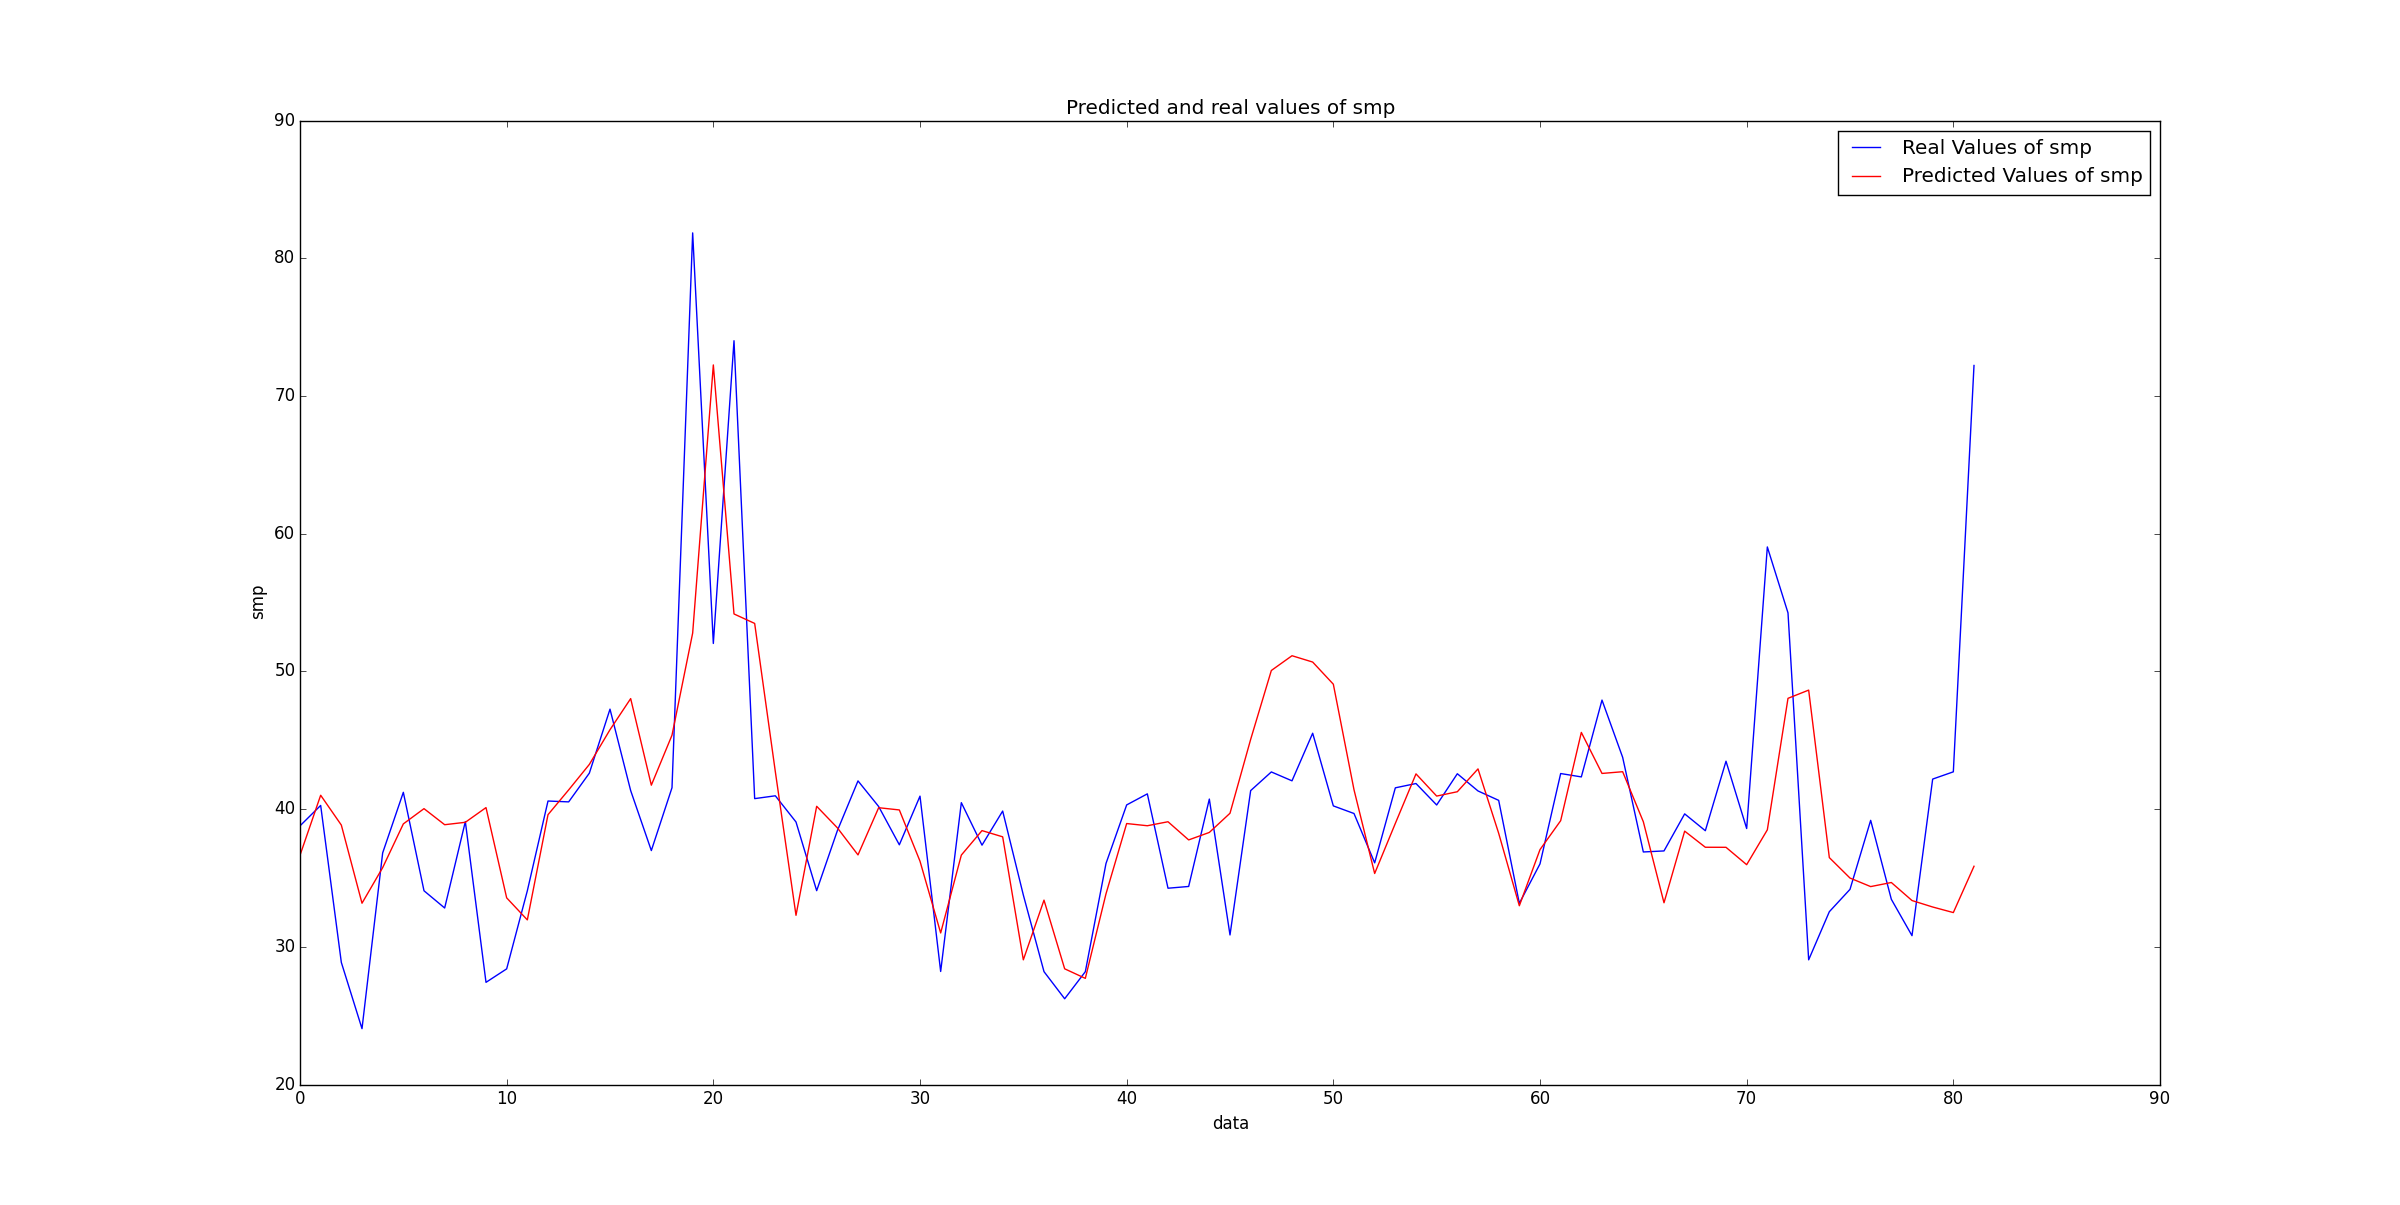
\includegraphics[width=1.3\textwidth]{fig/t-2.png}}%
  \caption{\tl{Random Forest - lag} ��� \tl{t-2}}
  \label{figure:57}
\end{figure}

\begin{figure}
  \makebox[\textwidth][c]{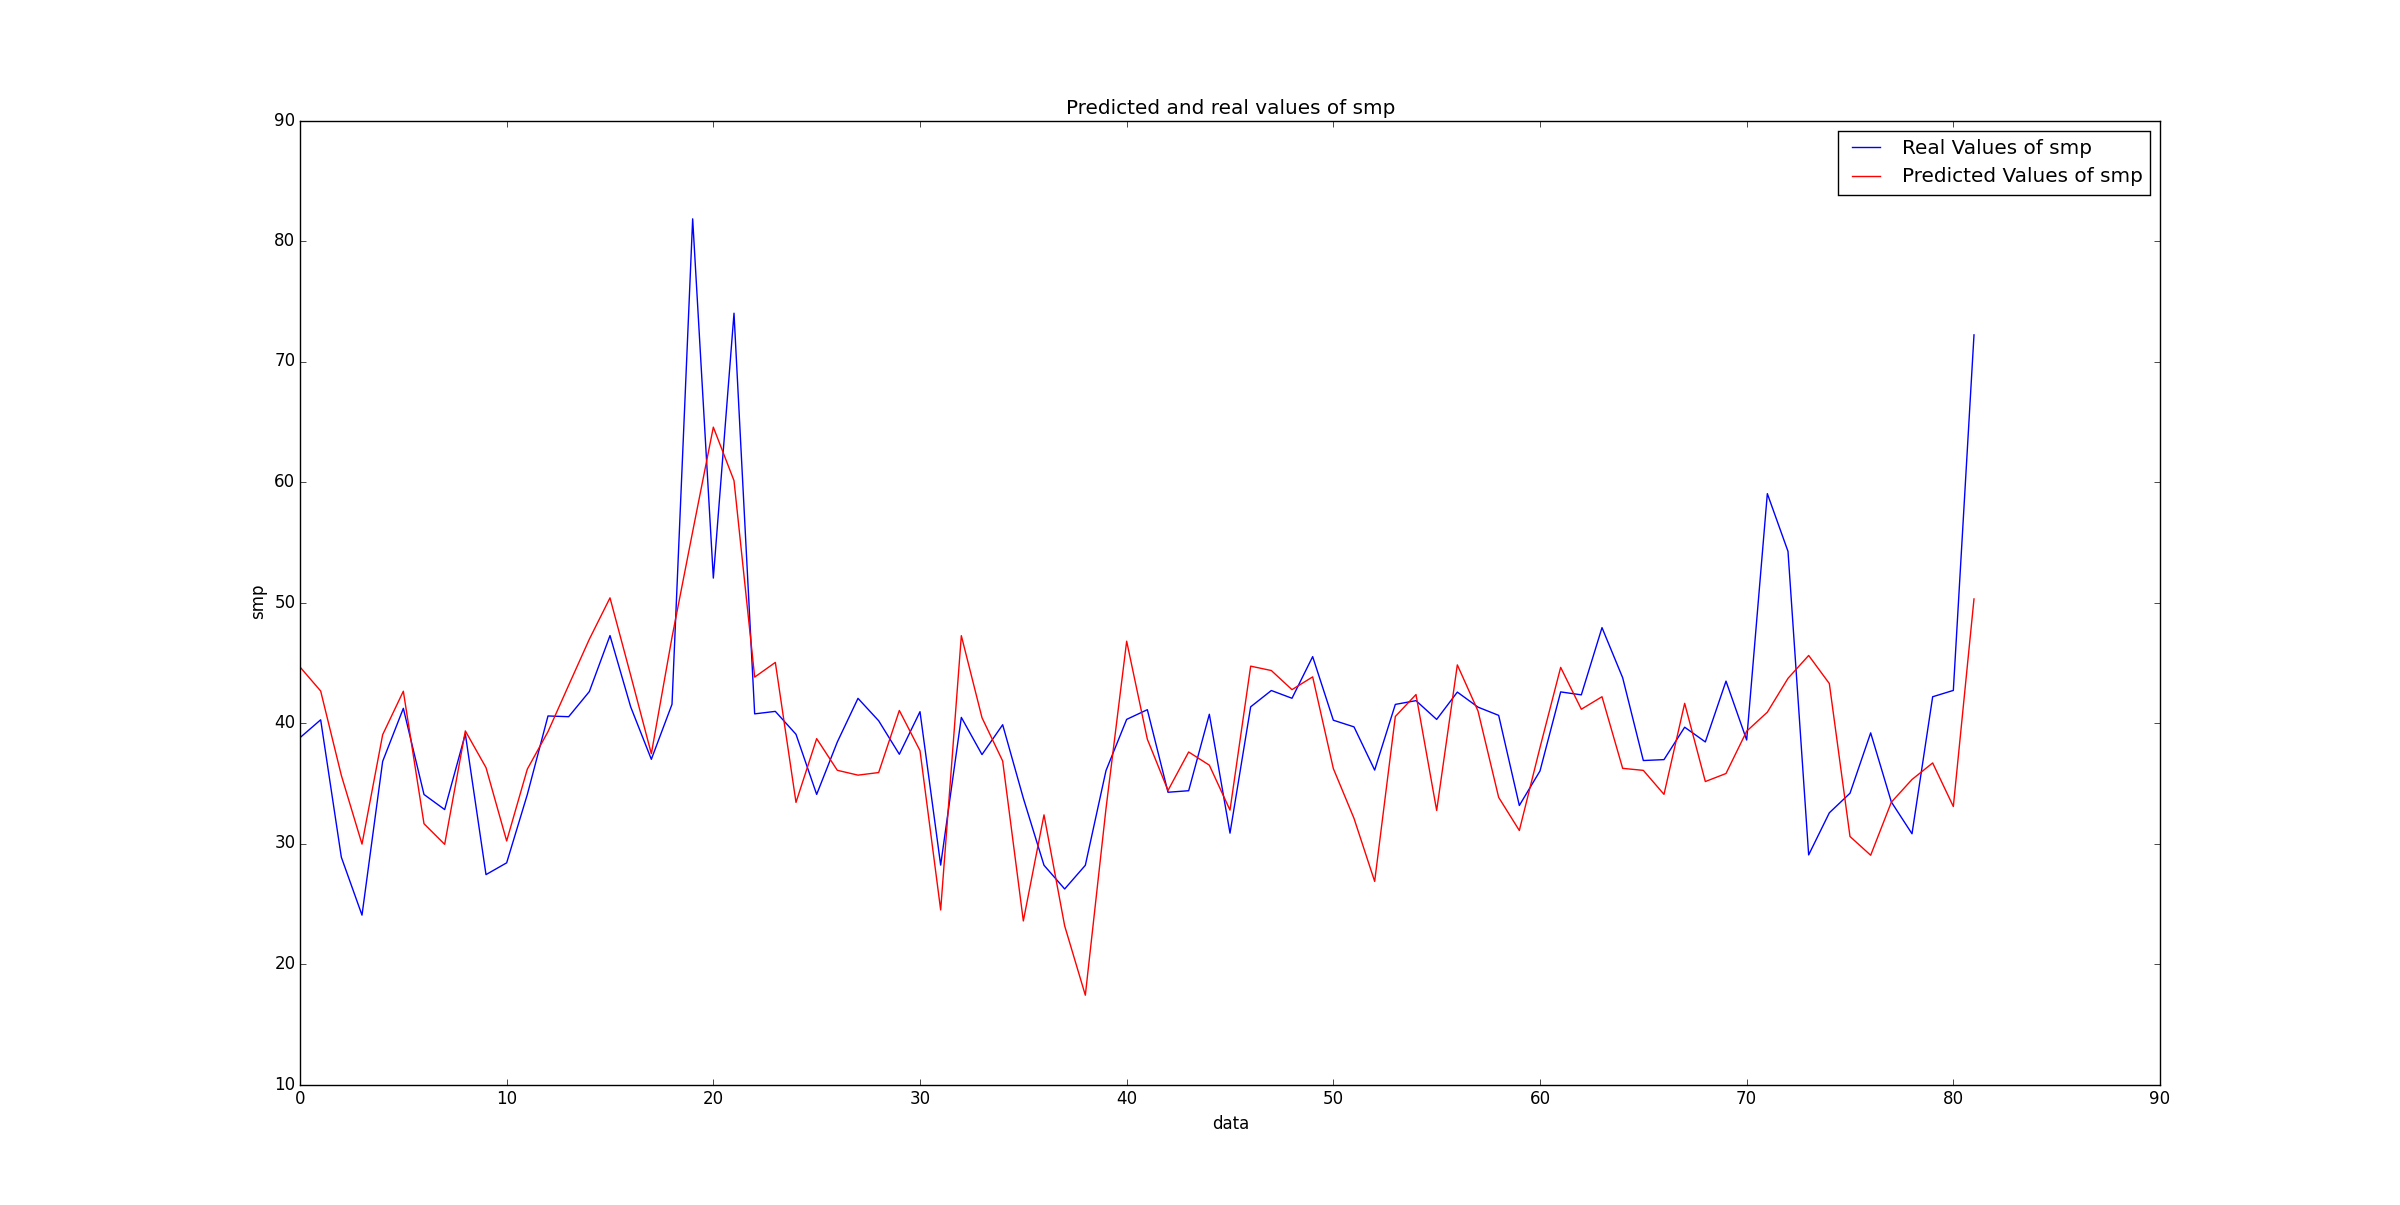
\includegraphics[width=1.3\textwidth]{fig/mars_t-2.png}}%
  \caption{\tl{MARS - lag} ��� \tl{t-2}}
  \label{figure:58}
\end{figure}

\section{������� �����������}

���� ����������� ��� ����������� ���������������� ��� �� ����� ���������� �� \tl{lagged values} ��� $t-2$. ���������������� 3 ������������ ������ ������������ ���������, ���� ������� ��������� ��������.

\subsection{����������� \tl{train} ��� \tl{validation sets} �� ��� ��� ����������}

������ ���������� ���� ����� ����������� �� \tl{train} ��� \tl{test sets} ��� �������� ��� ��� ����������. �� ��� ����� \tl{train set} ��������� ��� ��� ���� ��� �� 100 ����� �������� ��� �� �������� ���� \tl{test set}, ��� �������� ���� ���� ���� 100 �������� �������� �� \tl{train set} ��� �������� ���������� �� \tl{test set} ����� ��� ����� ������ 100 �������� ��� \tl{test}. ��� ����� \ref{figure:59} �������� � ���������� ��� ������������. �� ���� ���� ����������� �� ������� �� �������� ��� \tl{Mean Accuracy, Variance, MAE, MSE} ���� ��� ��� �������������� ��� ���������� ��� ���������� �������������� �������� ����������� ��� ���������� �� ����� �� �� ���������� ������.
\newpage

\begin{figure}
  \makebox[\textwidth][c]{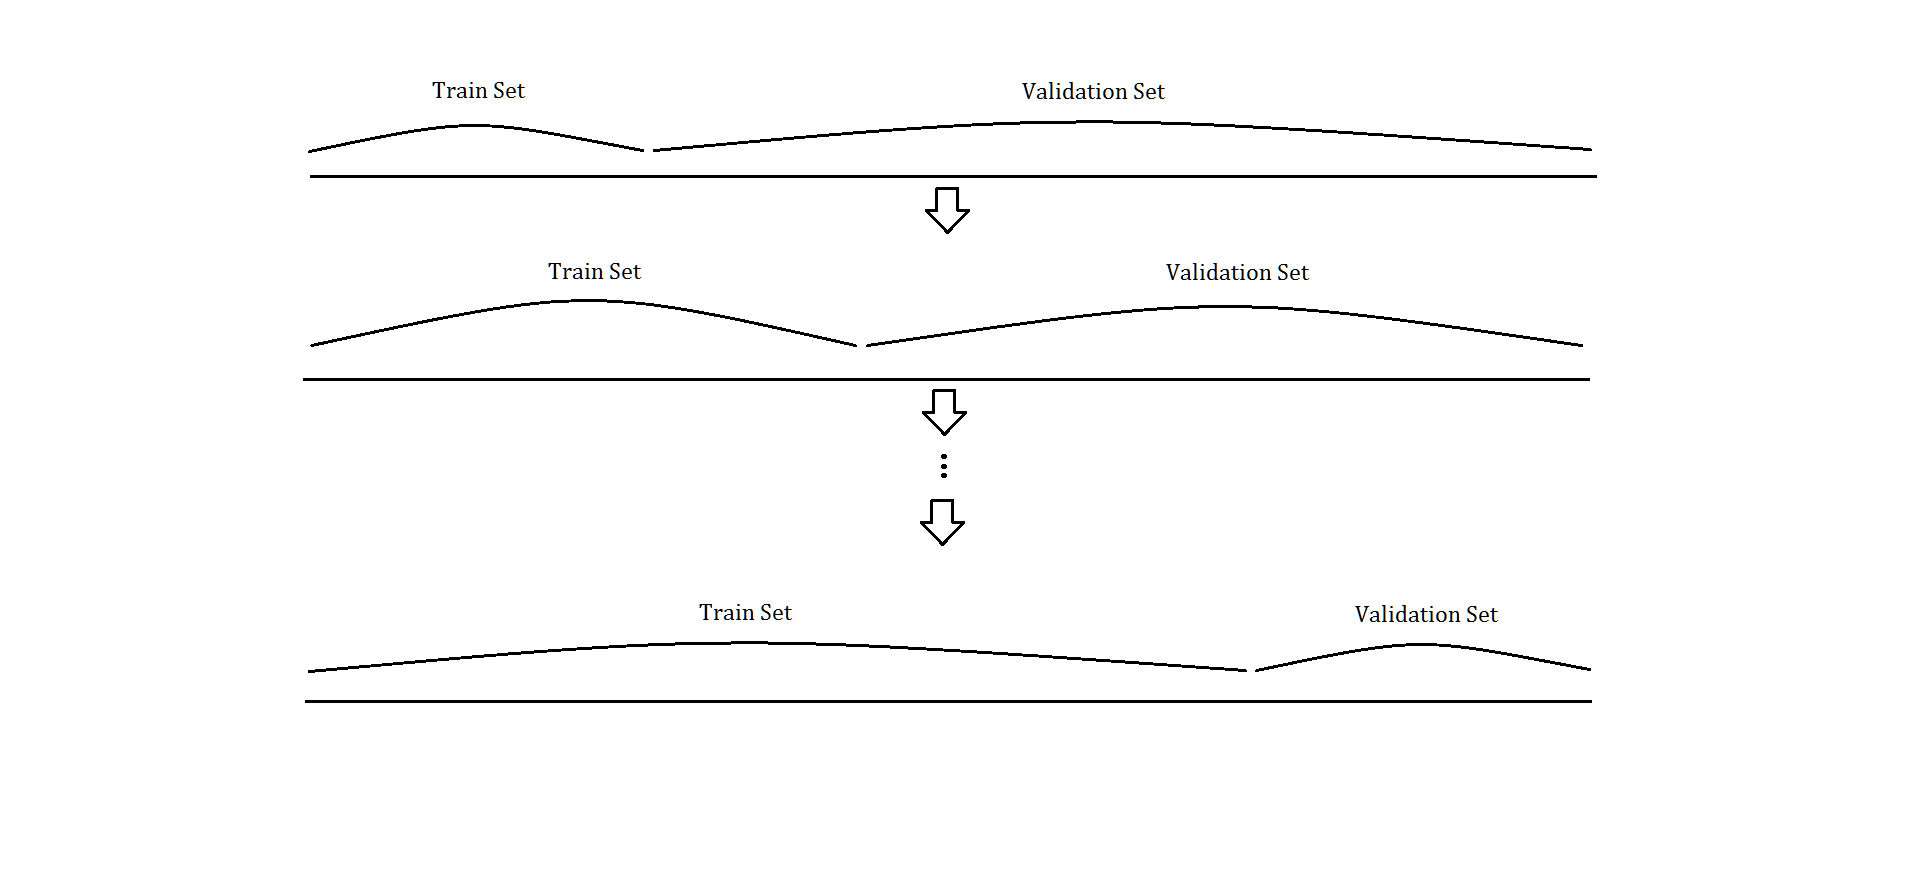
\includegraphics[width=1.3\textwidth]{fig/1.png}}%
  \caption{������� ��������� 1}
  \label{figure:59}
\end{figure}

\begin{figure}
  \makebox[\textwidth][c]{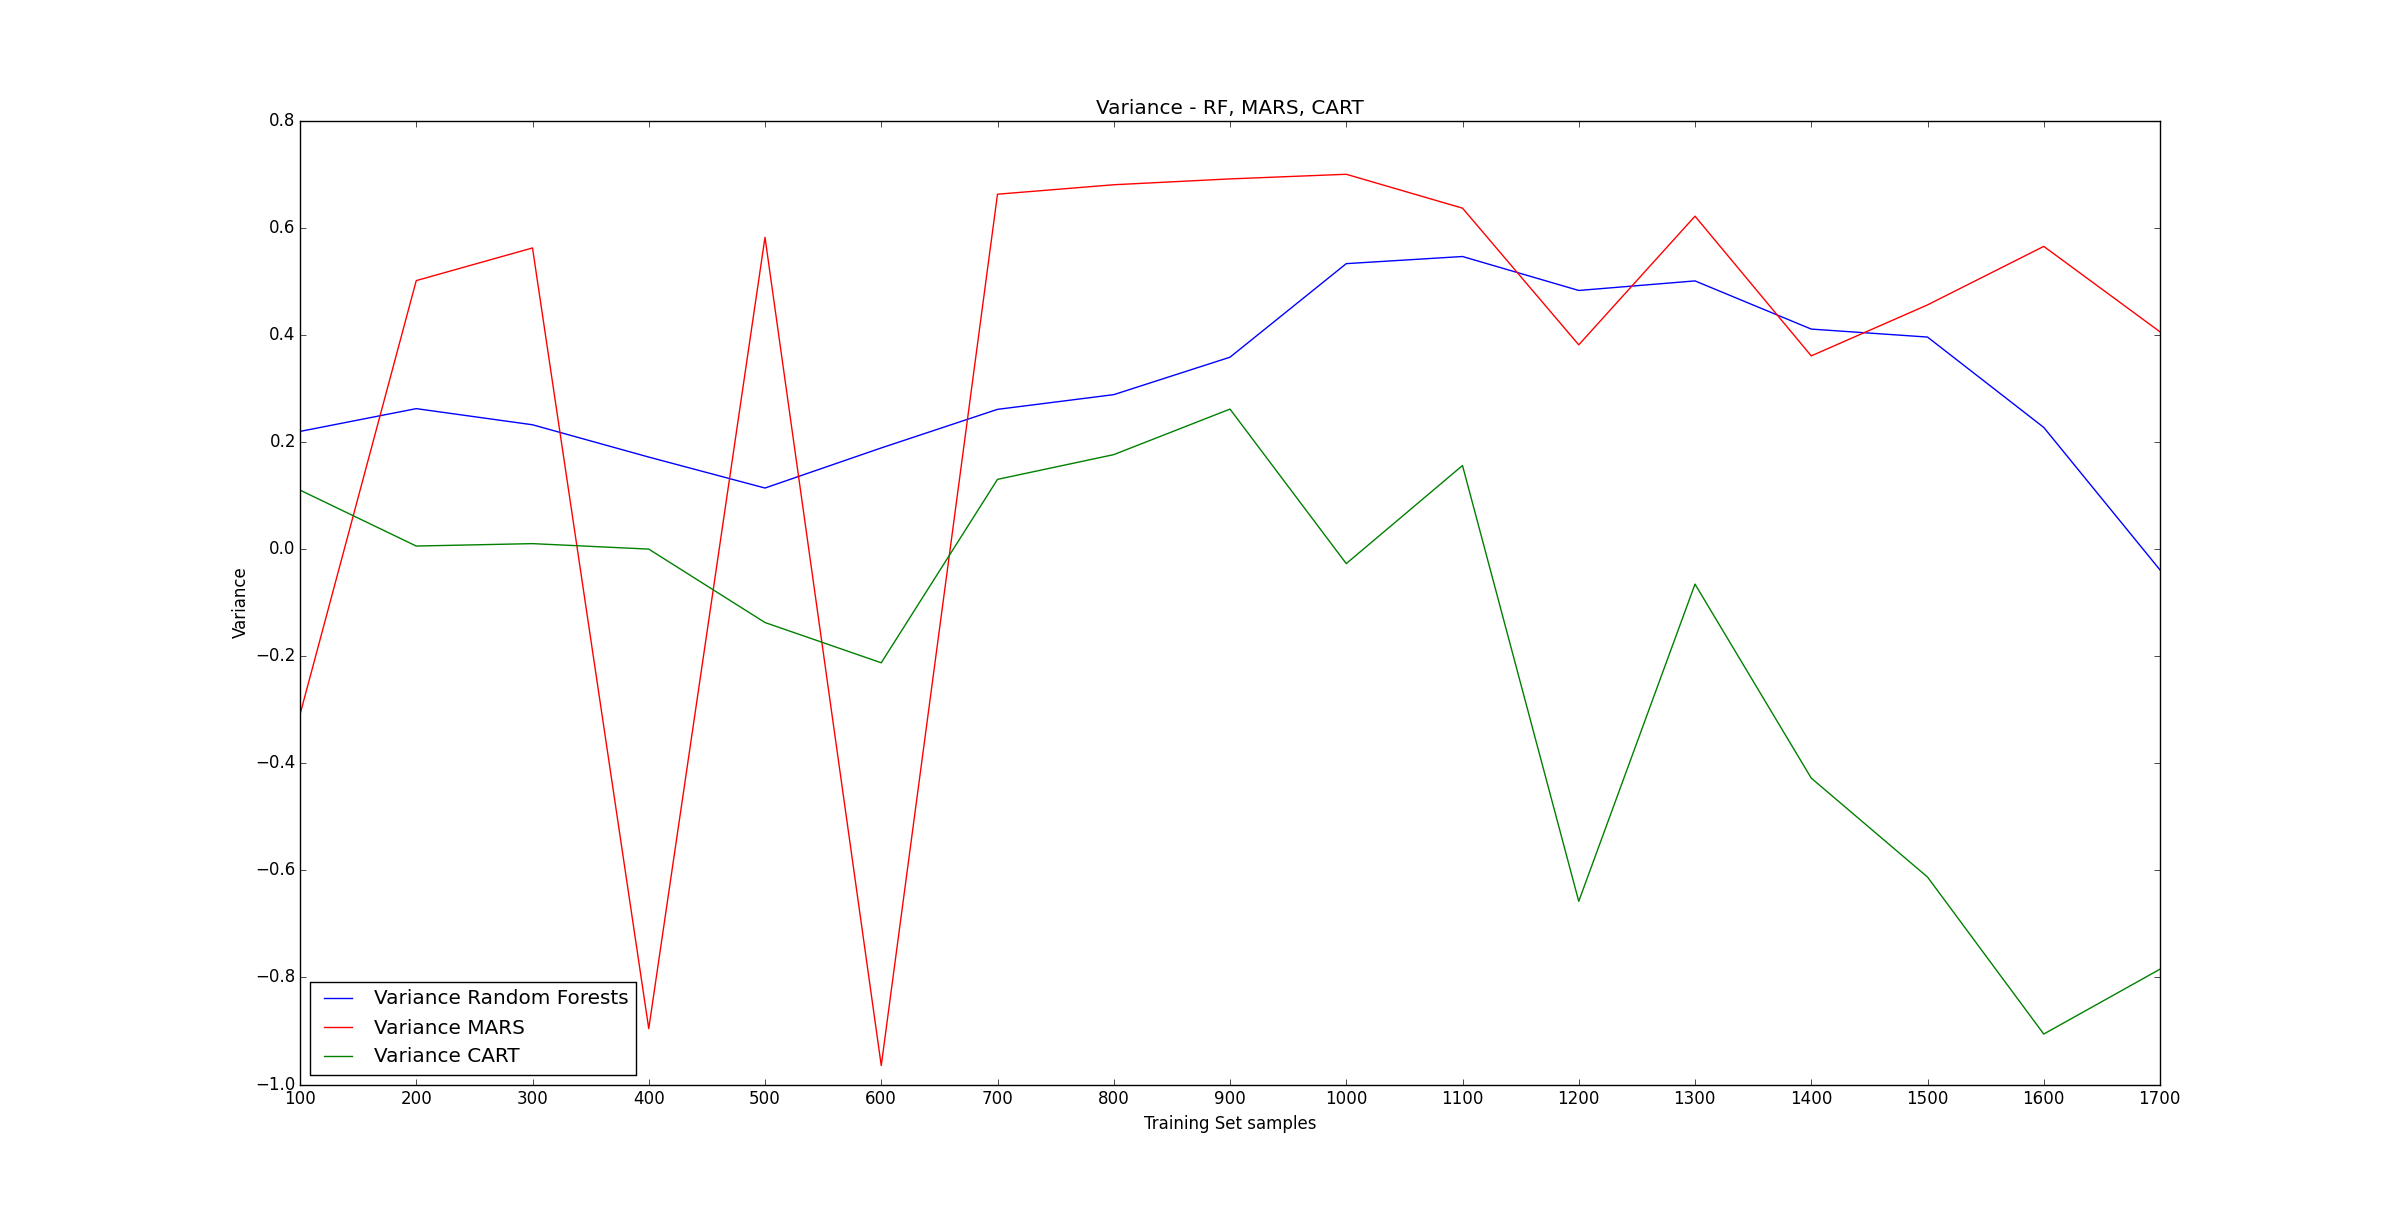
\includegraphics[width=1.3\textwidth]{fig/variance1.png}}%
  \caption{\tl{Variance} - ������� 1�}
  \label{figure:65}
\end{figure}

\begin{figure}
  \makebox[\textwidth][c]{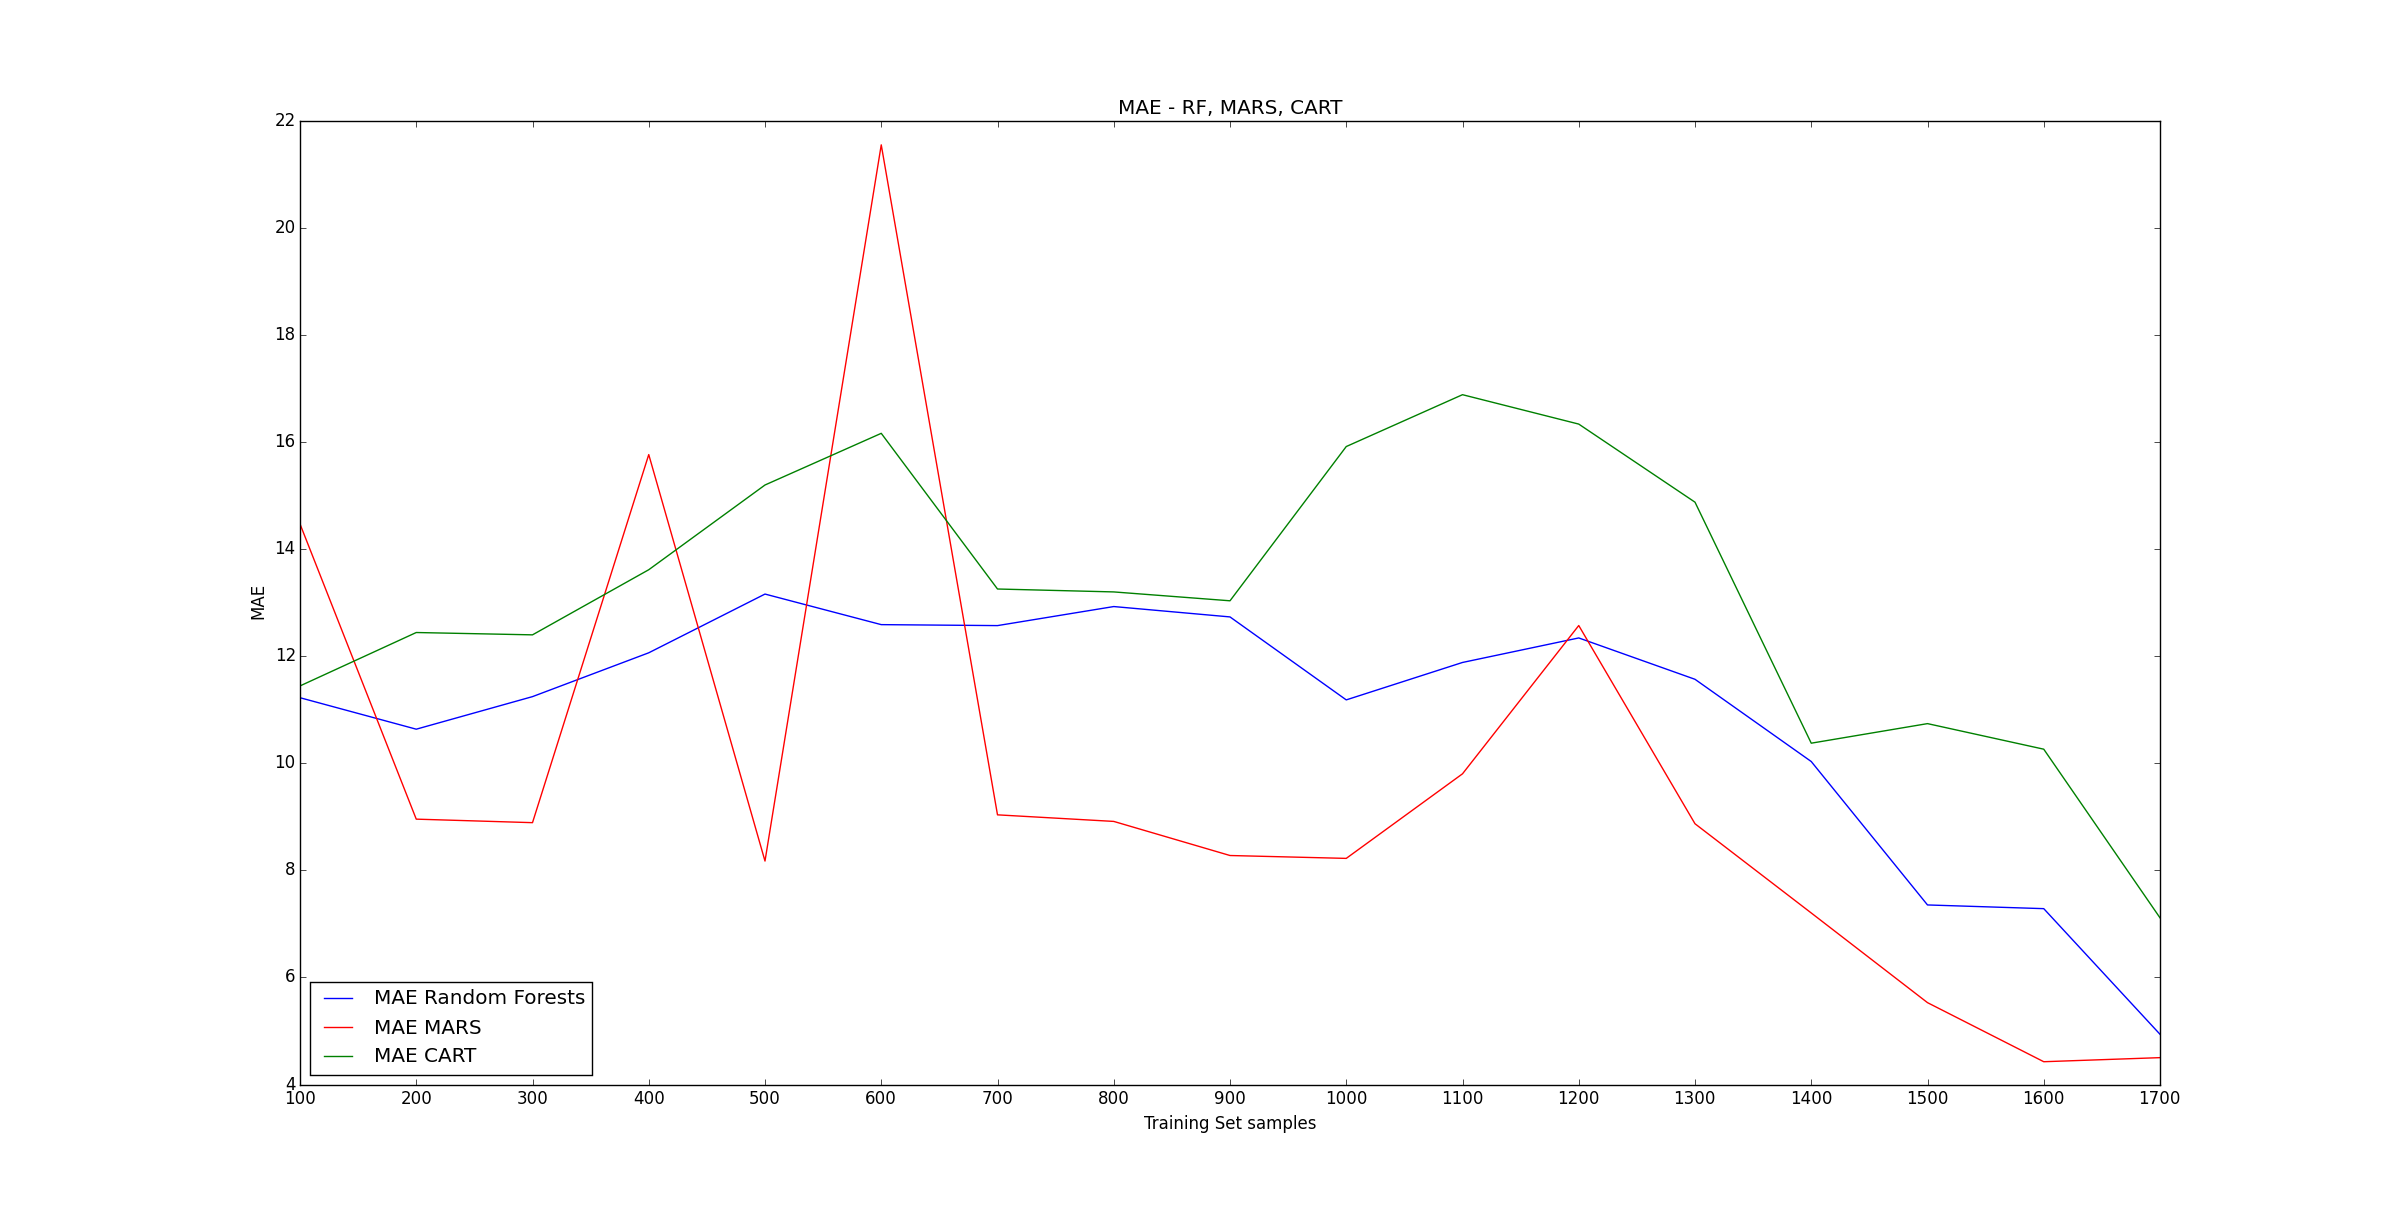
\includegraphics[width=1.3\textwidth]{fig/mae1.png}}%
  \caption{MAE - ������� 1�}
  \label{figure:66}
\end{figure}

� ���������� \tl{MARS} ���������� ���� ���� ������������, ������� �� ������ ������ ������ �������� 70\%. ���������� ���� ��� ����������� �������� ���� ���� ���� �������. �������� � ���������� \tl{Random Forests} ���� ��� ���������� �� ��� ��� �������� ���� �� ��������� ������� �� ����� �� ��� \tl{MARS} �� ������ ������. �� ���������� ����������� �� �������� ������������ ��� \tl{train set} �������� 1000, �� ����� �������� ���� ���� ��� ������� ����� ��� ����������� ���� �� ������� ���������� �����. ��� ����� \ref{figure:51} ��� �������� �� \tl{SMP}, �� �������� \tl{train set} ��� ��� �������� ��� ��������� ����� ����� ��� ��� ����� ���� 2009 ��� ���� ��� 2011. ���� �������� ��������� � ���������� \tl{MARS} ���� \tl{variance} ��� 57\% ��� ������� �������� ������������. �� ���� \tl{training set} ���� ���������� ������ ���������� ���������� �����.

���� ����� ��� ������������� ��� ����������, ���� ���� ��������� \tl{Random Forest} ��� ��� ���� ��������� \tl{MARS} � ��� ��������� ��������� ���� �� \tl{SMP(t-1)} ������������� ��� �� \tl{ngas}. ��� \tl{Random Forest} ������� ��� ��������� ��������� ���� �� \tl{smp(t-2)} ��� ������ ������� �� \tl{load\_forecast}, \tl{ngas(t-1)}, \tl{waip} ��� \tl{waters}. ���� ��������� \tl{MARS} ����� ������������� ��������� ���� �� \tl{ngas(t-1)} ������������� ��� �� \tl{smp(t-2)}, \tl{load\_forecast} ��� \tl{waip}. �������� � ������������� ��� ���������� ����������� ������ ���������� ����� ��� �����������.

\subsection{����������� \tl{train sets} - ���� \tl{test set}}

���� ������ ��� \tl{validation set} ��� �������� [1600:] ��� ����������� \tl{train sets} �� ����� ������� ��� �������� [:1600-\tl{x}], $x_0 = 0$ ��� \tl{x} ������� ��� 100. �� �������� �������� ��� ����� \ref{figure:60}. 

\begin{figure}
  \makebox[\textwidth][c]{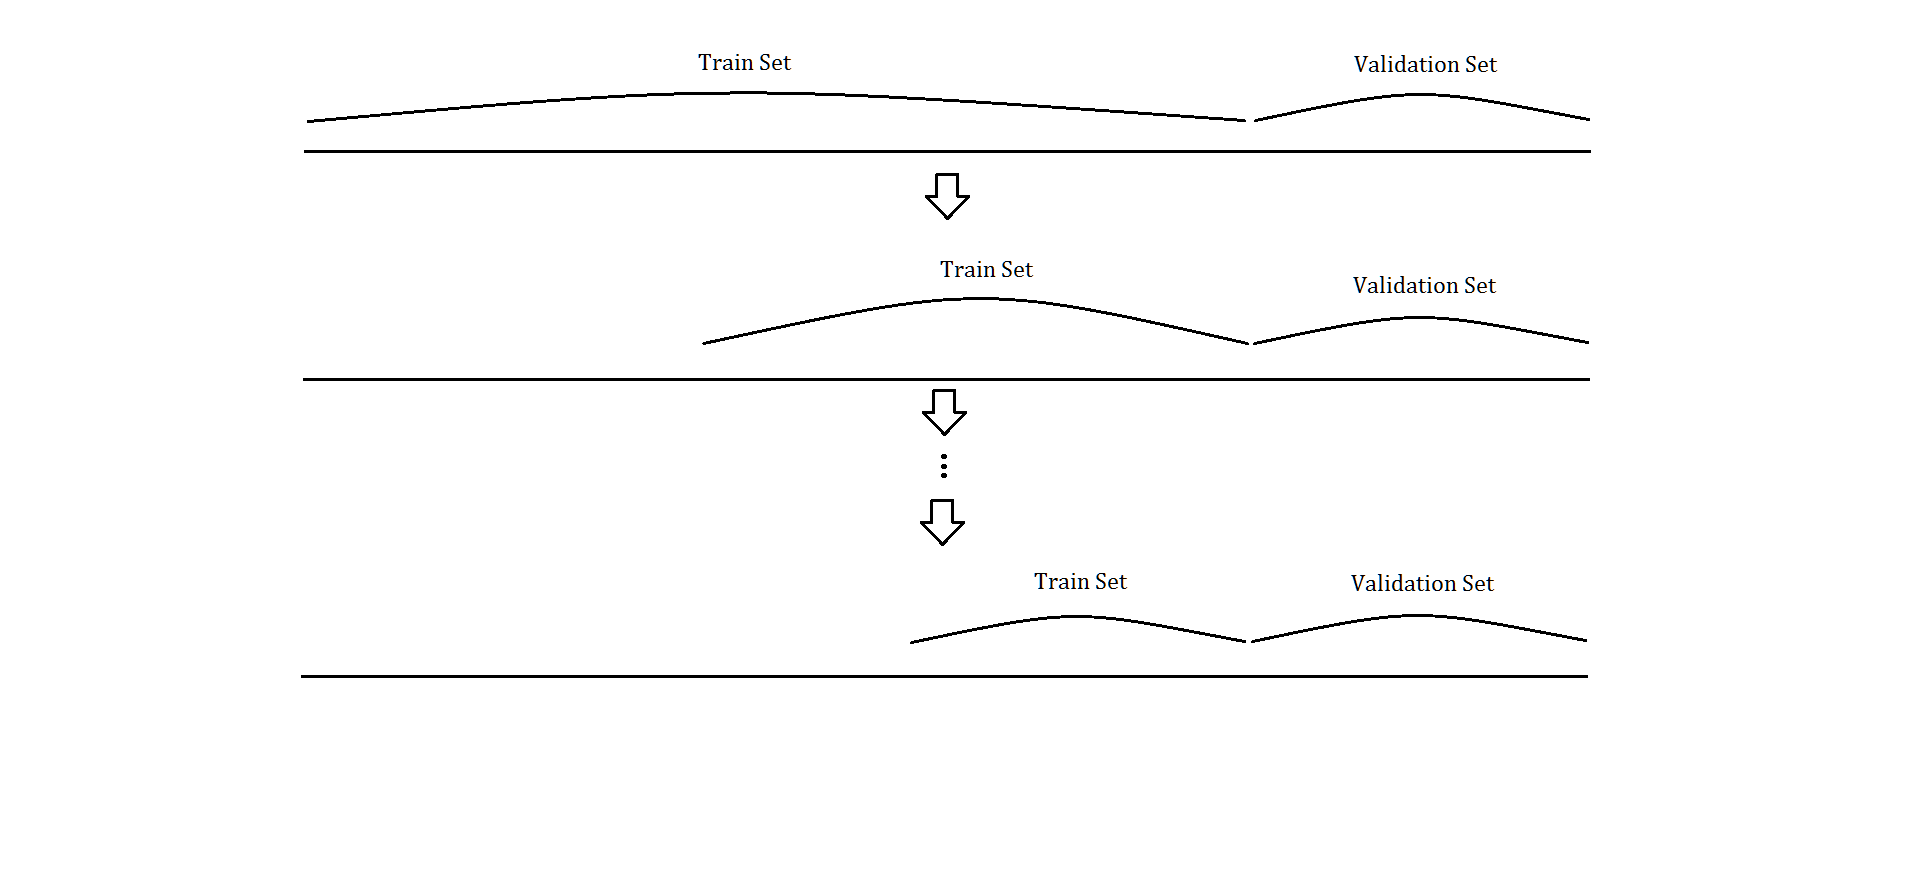
\includegraphics[width=1.3\textwidth]{fig/2.png}}%
  \caption{������� ��������� 2}
  \label{figure:60}
\end{figure}

\begin{figure}
  \makebox[\textwidth][c]{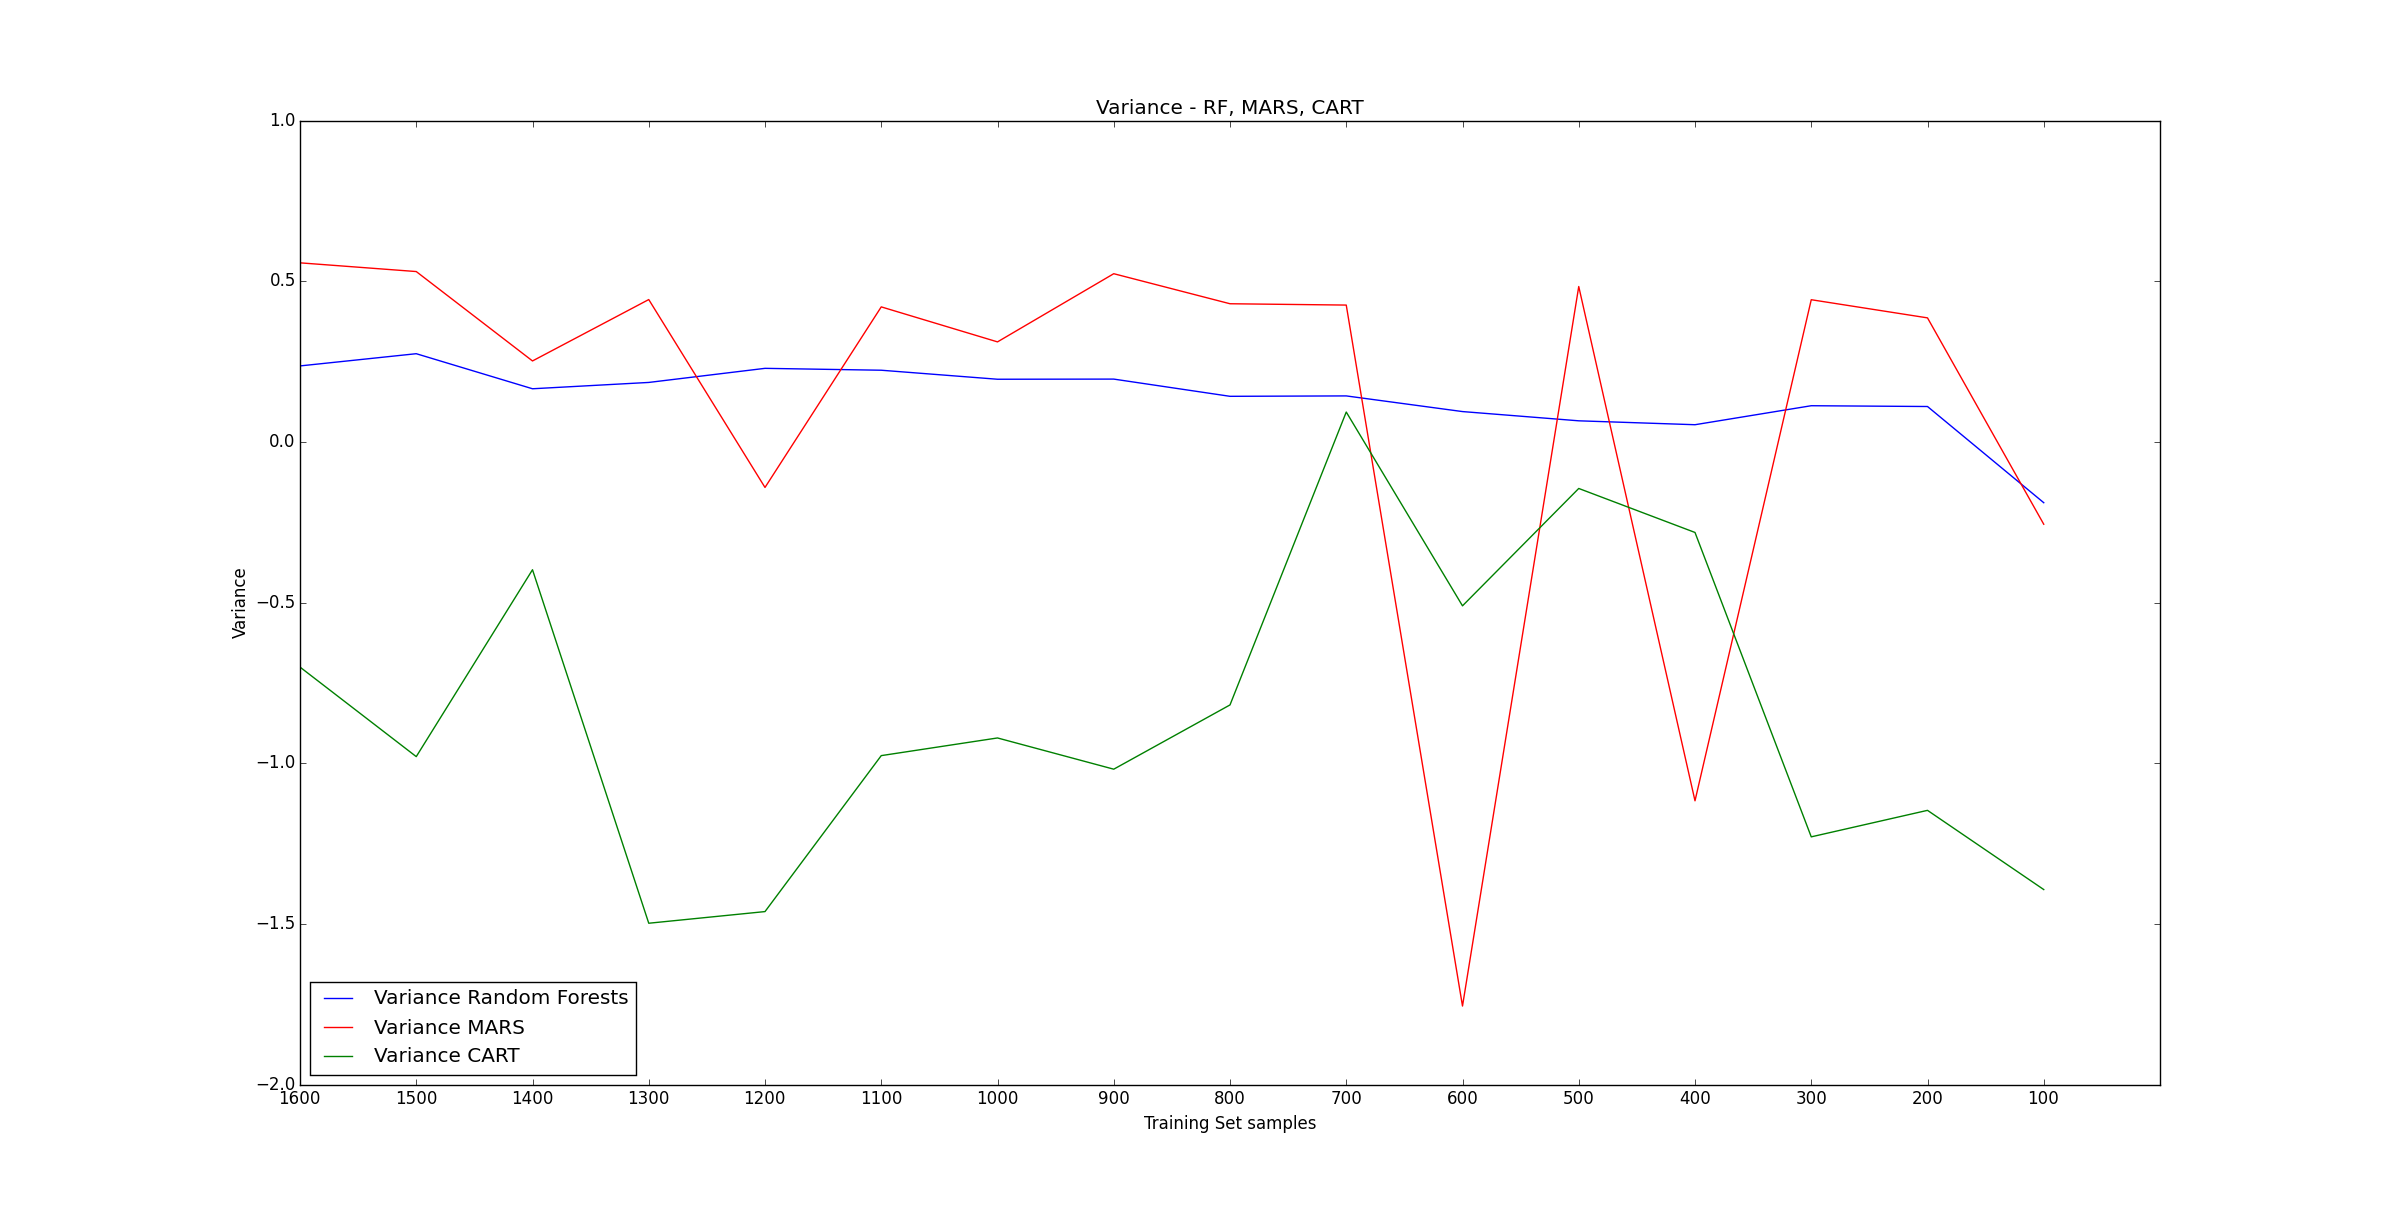
\includegraphics[width=1.3\textwidth]{fig/variance2-2.png}}%
  \caption{\tl{Variance} - ������� 2�}
  \label{figure:68}
\end{figure}

\begin{figure}
  \makebox[\textwidth][c]{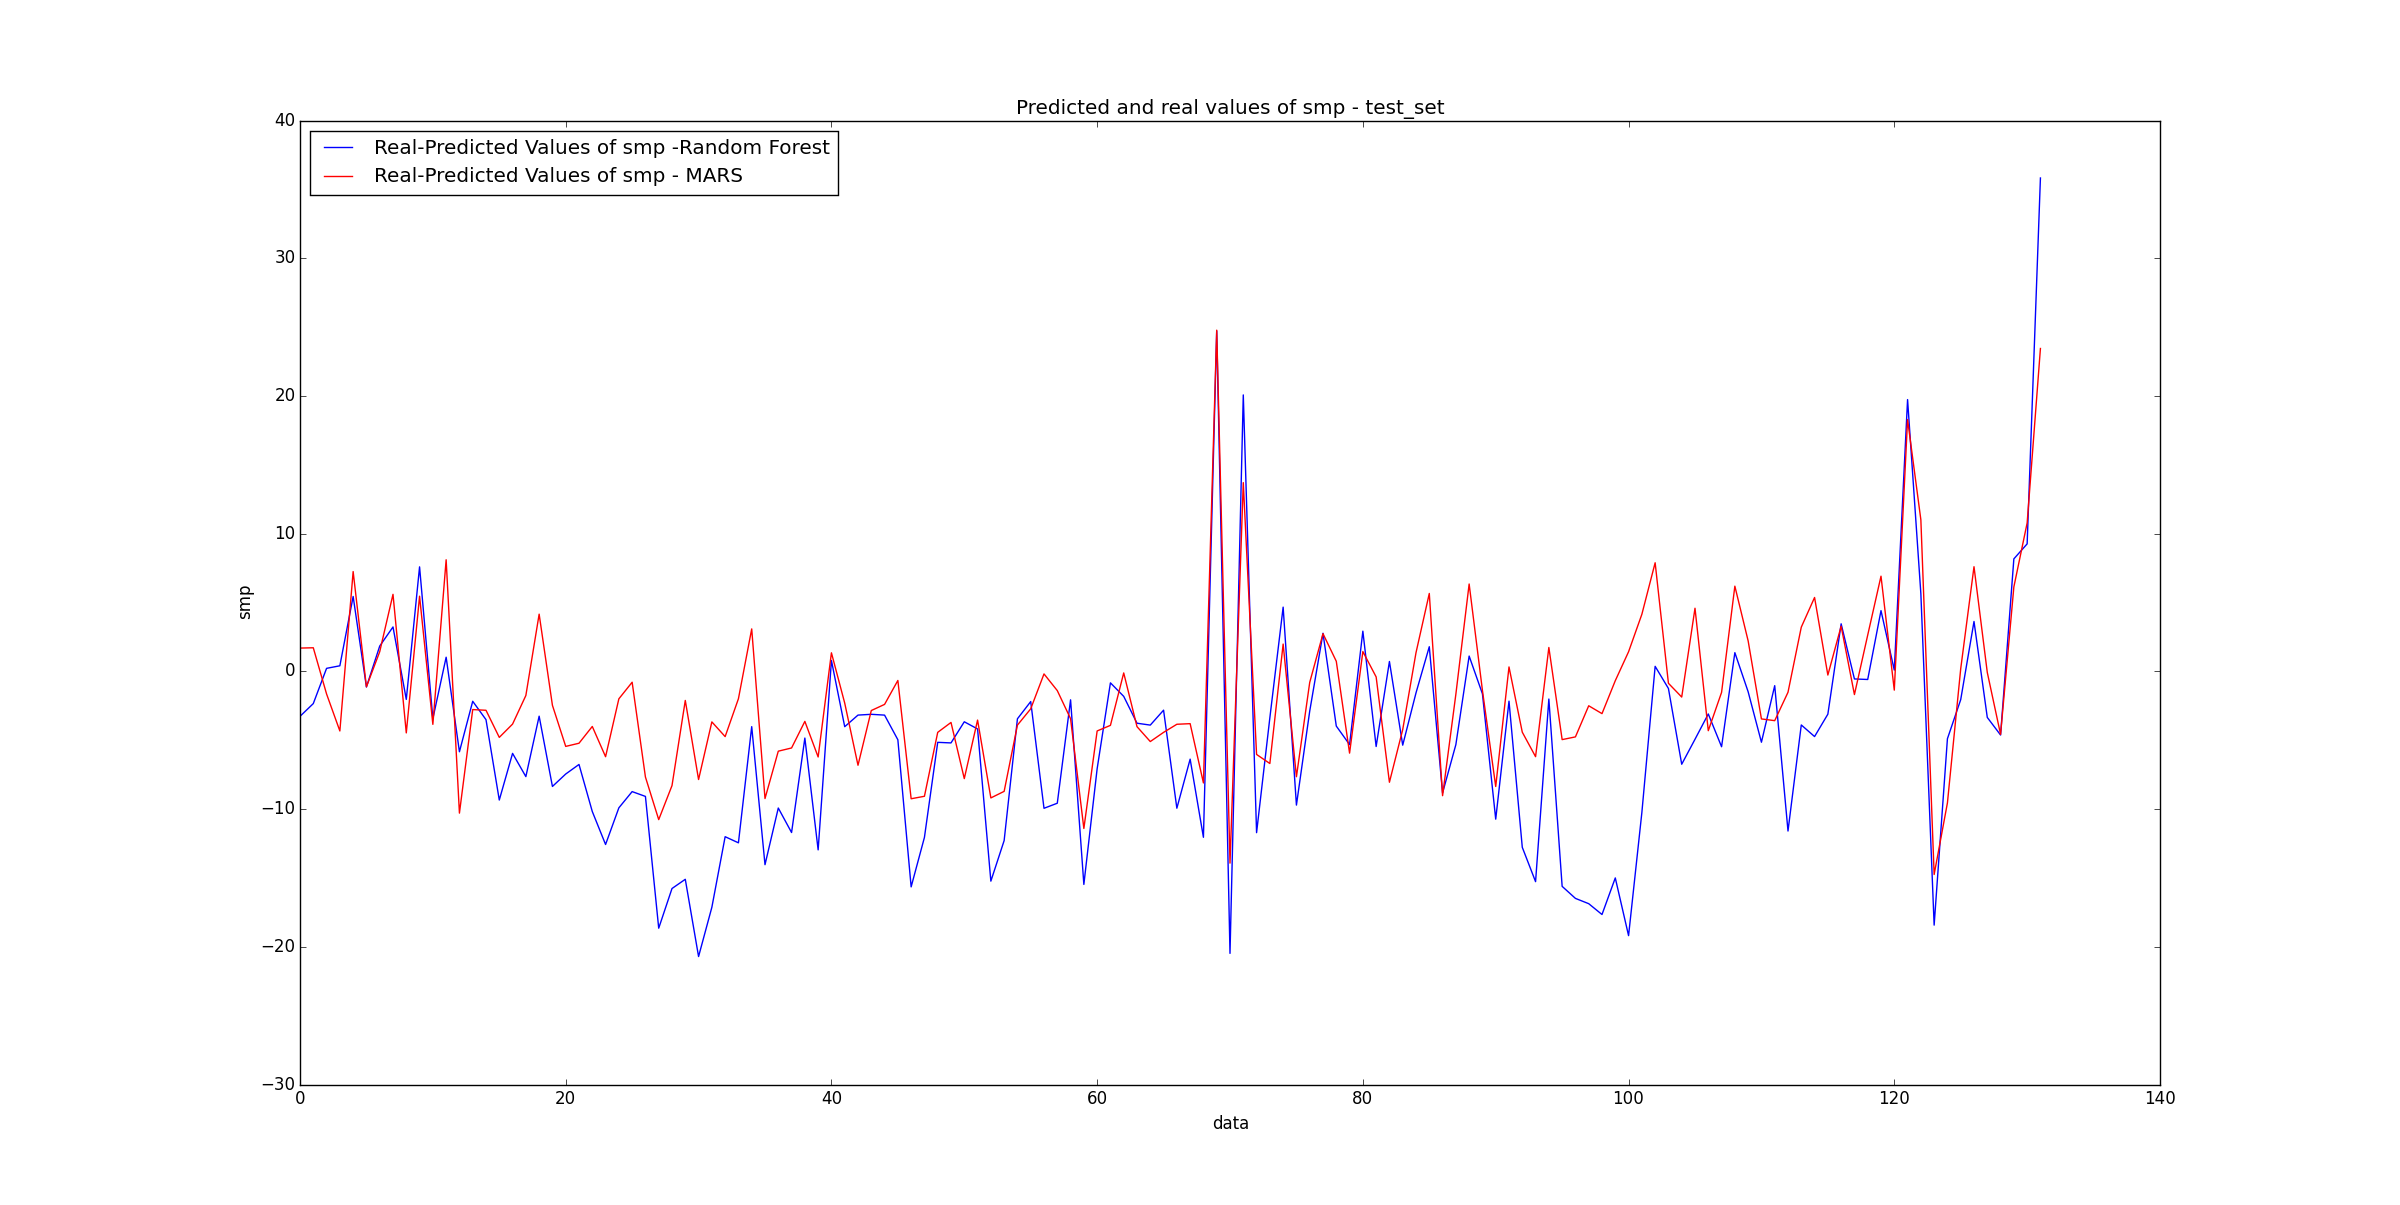
\includegraphics[width=1.3\textwidth]{fig/figure_16--1.png}}%
  \caption{\tl{Random Forest} ��� \tl{MARS} - \tl{Real - Predicted}}
  \label{figure:67}
\end{figure}

�� ������������ ��������� ��� ����� \ref{figure:68} ��� ����� �������� �� ����. ������ �� ������ ������ ��������� ����� ��� \tl{MARS}, ���� �� ������ ���� ����� �����������. �� \tl{Random Forest} ������� ������ ������������ ��� �� \tl{MARS} ������� �� �������� ������������ ��� \tl{training sets} 1500 ��� 1600 �����, ������ ��������� ��� ���������. � ������������� ��� ���������� �� ���� �� �������� ��������� ���� �� ���� ��� ����� ��� �����������. ������ ����������� ��� ��� � ���������� \tl{CART} ��� ������� ����� ������������ ��� ����������.

��� ����� \ref{figure:67} ������ ��� �������� ��� ����������� ��� ��� ������������ ����� ��� ���� ����������� \tl{Random Forest} ��� \tl{MARS} ��� ��� \tl{train set} 1600 �����. ����������� ��� � ���������� \tl{MARS} �������� ����� �������� ������������. �� ���������� �������� ����� �� ������ �������� ��� ��� ���������� ��� ���� ������ ��� �������� ������������ �������� �����������.


%\subsection{����������� \tl{train} ��� \tl{validation sets} �� ��� ��� ���������� (���������� 1)}
%
%��� ������ ��� ���� ���������� ��� ����� ���� ����� ��������� �� ��� ������� ��� ������� \tl{test} ��� ����������� ����� ��� \tl{SMP} �� ���� ��� ��� ���������. �� ������ ����� ���� �� ���� ��� � ���������� �������� ��� ����� \ref{figure:61}.
%\newpage
%\begin{figure}
%  \makebox[\textwidth][c]{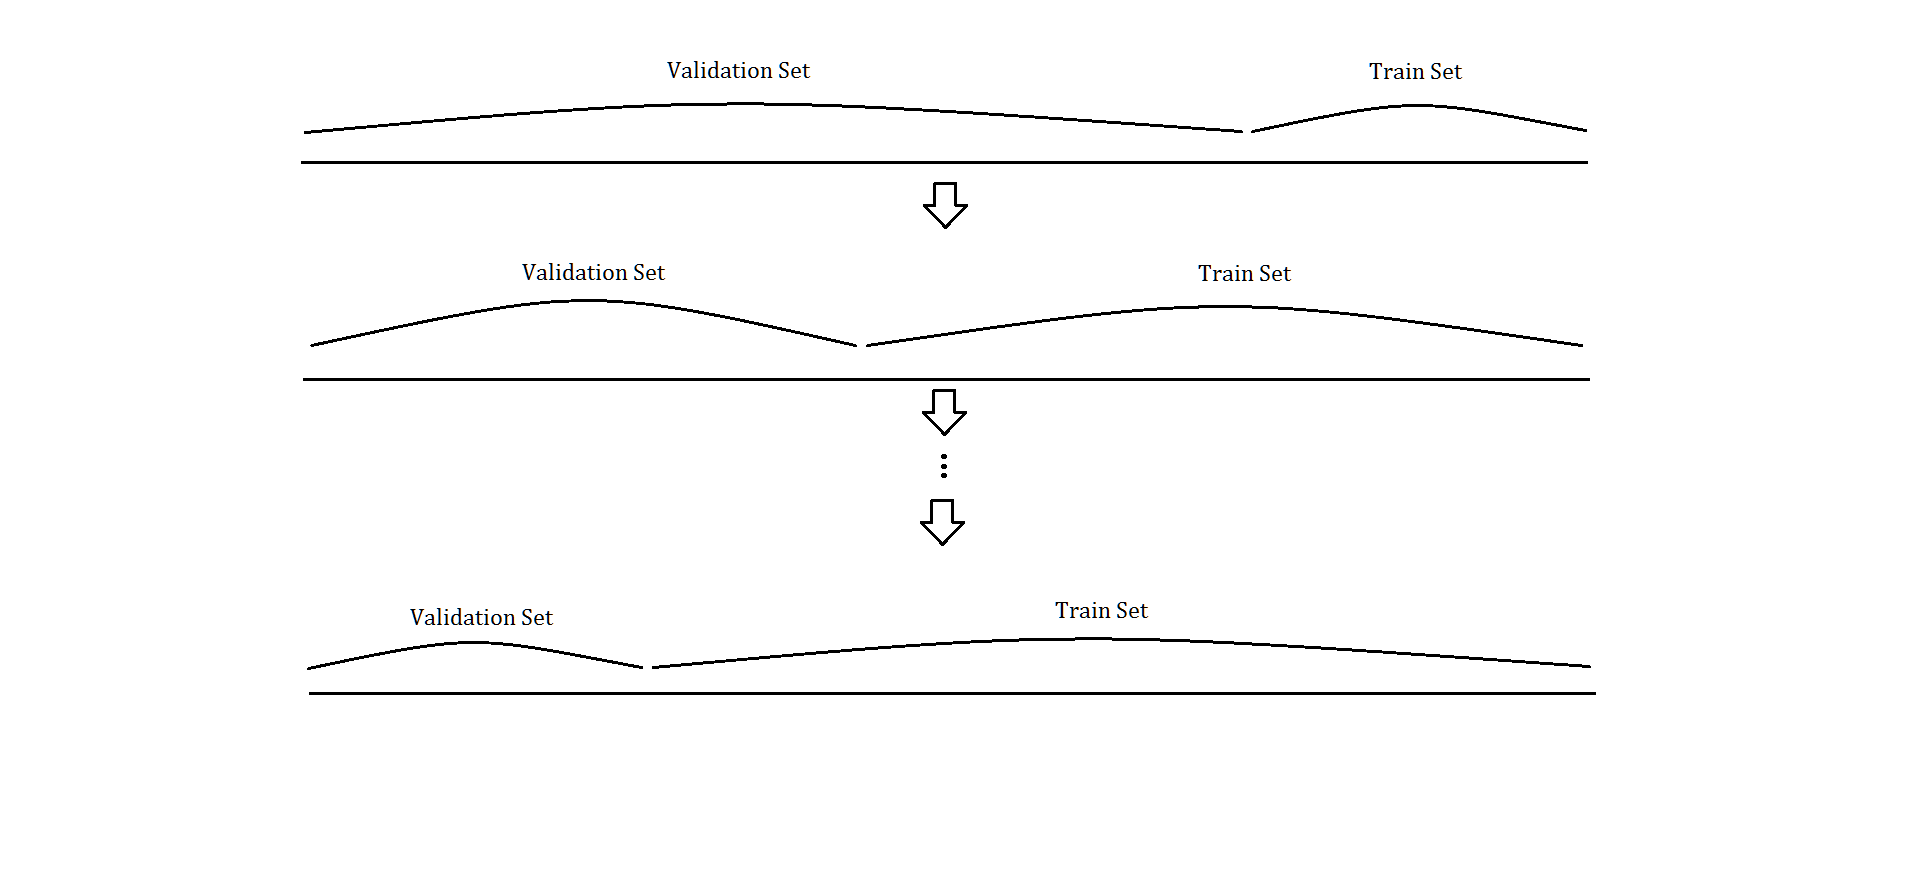
\includegraphics[width=1.3\textwidth]{fig/3.png}}%
%  \caption{������� ��������� 3}
%  \label{figure:61}
%\end{figure}
%
%\begin{figure}
%  \makebox[\textwidth][c]{\includegraphics[width=1.3\textwidth]{fig/variance3-3.png}}%
%  \caption{\tl{Variance} - ������� 3�}
%  \label{figure:69}
%\end{figure}
%
%\begin{figure}
%  \makebox[\textwidth][c]{\includegraphics[width=1.3\textwidth]{fig/figure_16-3.png}}%
%  \caption{\tl{Random Forest} ��� \tl{MARS} - ������� 3�}
%  \label{figure:70}
%\end{figure}
%
%���� ��� ���� ������������ ����������� � ���������� \tl{MARS} ����� ��� ������� ���� �� ������������ ������ ������ �� ������� �� �������� ������������. � ���������� \tl{Random Forest} ������� ���������� ���� ����� ���������� ���� ������������ ��������� ��������� ����� ��� 70\%. � ���������� \tl{MARS} ������ �� 77,5\% ��� �� ���� ����, ���������� ����������. ��� ����� \ref{figure:70} ������ �� ������������ ���� ��� �� ������������ \tl{iteration}. ��� ������ �� �������� ��� � �������� ���� ���������� �� ����� �� ���� ���� ��� ������������ ��� ������� ��������� ��� \tl{SMP}. ���� ����� ��� ������������� ��� ����������, �� ���� ��� ��������� ������ �������� ������������� ��� ���������� \tl{waters} �� ����� �� �� \tl{load\_forecast}, ���� ���� �� ��� ���������� ���������� ����� �� \tl{SMP(t-1)} ��� \tl{ngas}. 
%
%\subsection{����������� \tl{train}, ���� \tl{test} (���������� 2)}
%
%������� ���� ���� � ���������� ������� ���� ������������� \tl{test set} ��� ������ �������� �� ����� ����� ��� �������� [100:400]. �� \tl{train sets} ���������� ��� ��� �� �������� ��� ����������� ��� ��������� ��� �� �������� [400:500]. 
%\newpage
%\begin{figure}
%  \makebox[\textwidth][c]{\includegraphics[width=1.3\textwidth]{fig/4.png}}%
%  \caption{������� ��������� 4}
%  \label{figure:62}
%\end{figure}
%
%\begin{figure}
%  \makebox[\textwidth][c]{\includegraphics[width=1.3\textwidth]{fig/var4.png}}%
%  \caption{\tl{Variance} - ������� 4�}
%  \label{figure:71}
%\end{figure}
%
%\begin{figure}
%  \makebox[\textwidth][c]{\includegraphics[width=1.3\textwidth]{fig/analysi4.png}}%
%  \caption{\tl{Random Forest} ��� \tl{MARS} - ������� 4�}
%  \label{figure:72}
%\end{figure}
%
%\begin{figure}
%  \makebox[\textwidth][c]{\includegraphics[width=1.3\textwidth]{fig/marsnice.png}}%
%  \caption{\tl{MARS} - ������� 4�}
%  \label{figure:73}
%\end{figure}
%
%�� ������������ ����� �������� �� ����. � ���������� \tl{Random Forest} ����� ������� ������������ ����� ��� 60\% ��� � ���������� \tl{MARS} ����� ���� ������������ ���� �� ������������ ������. �� �������� ���������� ����� 65.9\% ��� ��� ��������� \tl{MARS} �� ����� ������������� ��� \tl{training set} �������� ����� 300 ���������. �� ���������� ���� ����� ������ ��������� ��� ����������� ��� ����������: �� \tl{validation set} ������ ��� ����� ��� 2009 ��� ������� ���������� 2010 ���� �������� ��� ����� \ref{figure:51}. �� ������ �� �� ���������� \tl{accuracy} �������� ������ ���� ��� �������� ��������� 2011. �� �������� ��� ��� �������� ����� ��������� �� �������� �������������� �������� � ����� �������� ���� ����� ����������.
%
%���������� ������������ �� \tl{importances} ��� ����������: ������ ��� ��������� ��������� � ��������� \tl{SMP(t-1)} ���� ���� ������������� ��� 21.5\% �� ����� �� 45\% ���� ������������ �����������. ���� ��������� ��� ������� ��� ������ ���������� ����������� ����� �� \tl{lagged} ���������� ��� ����� ���� ����������. ������� ������� �� \tl{ngas} �� �������� ������������� �� ����� �� ���� (���� ��������� �������������� \tl{SMP(t-1)}) ��� ���� �������� ������ �� \tl{SMP(t-2)} ��� \tl{load\_forecast}. � ���������� \tl{MARS} ������� ��� ������������ ���������� ��� ������������� ����� ��� ����� ��� ������������ ��� ���������� \tl{waters}, \tl{waters(t-1)}, \tl{lignite}, \tl{lignite(t-1)} ��� \tl{load\_forecast(t-1)} ������ 9 ���������� ��� ��� 32 �� ���� ���� ������ ����������. ��� ����� \ref{figure:72} ��������� �� ����������� ��� \tl{train set} ��� �������� [400:700].

\subsection{����� \tl{train-test sets} �� ��� ��� ����������}

��� ��� ������� �������� ��������� ���� ����������, ��������� \tl{train sets} ��� ������ [$x$:$x$+200] ��� \tl{test sets} ��� ������ [$x$+200:$x$+400], ���� $x_0=0$ ��� $x$ ������� ���� 100 �� ���� \tl{iteration}. ��� ����� \ref{figure:63} �������� ��� ���������� ��������. 

�� ������������ ����� �������� �� ����. � ���������� \tl{Random Forest} ���� ������ ���������� ���� � \tl{MARS} ������ �� ����� ��������� ���������� �� ������� ����������� ��� �� ������� ����� ������� ���������� �����. ��� ������������, � ���������� \tl{MARS} ���������� ��� �������� ������� ��� \tl{train set} [800:1000] ��� � \tl{Random Forest} ��� [900:1100]. ���� ����� ��������� ��� ��� ���� ��� ����������� �������� ��� �� ���� ������ ��� �����������. �� ������ �������������� ���� ��� ������� ����� � ����������� ����, ������ ��� ����� ���� ����������� ���� ����������. ��������� �� ������� ��� �� ���� ������� ������ ����� �������� ��� ����� ����� ����������� ��� ������ ������� ��� �����������.

������� �� ��� ��������������, � ���������� \tl{Random Forest} ������ �������� �������������� �� ����, �� ���� ��������� ���� �� ������ �� \tl{SMP(t-1)} ��� �� \tl{ngas} ���� ���� ��� ������ ��������� ��������� ������ �������� ���� ������������� ��� ���� ����������. ���� ��������� \tl{MARS} ���� �� �������� ����� ����� ��� �����������, �� �� \tl{ngas} �� ���������� ���� ��� ������� ���� ��� ���������� ��� �� ��� ������ ���� ���� �����. ��� ������ [1100:1300] ������� �� \tl{ngas} ��� �� \tl{SMP(t-1)} ��� ���������������� ������� ��� ��� ��������� ��� ������ �� ���������� ���� �� ������� �� ���������� \tl{load\_forecast} ��� \tl{waters}. ��� ������������ ������ ������ �������� ������������ ��� ��� ��� ��������� \tl{Random Forest} � ������ ������� ��� ��� ��������� ��������� �� \tl{load\_forecast} �� 36.5\%, 9.7\% �� \tl{ngas} ��� 8.9\% �� \tl{SMP(t-1)}. ��� ����������� ��� ���������� \tl{MARS} ��������� ��� ������� \ref{figure:76} ��� \ref{figure:77}.

\begin{figure}
  \makebox[\textwidth][c]{\includegraphics[width=1.3\textwidth]{fig/5.png}}%
  \caption{������� ��������� 3}
  \label{figure:63}
\end{figure}

\begin{figure}
  \makebox[\textwidth][c]{\includegraphics[width=1.3\textwidth]{fig/var5.png}}%
  \caption{\tl{Variance} - ������� 3�}
  \label{figure:74}
\end{figure}

\begin{figure}
  \makebox[\textwidth][c]{\includegraphics[width=1.3\textwidth]{fig/mae5.png}}%
  \caption{\tl{MAE} - ������� 3�}
  \label{figure:75}
\end{figure}

\begin{figure}
  \makebox[\textwidth][c]{\includegraphics[width=1.3\textwidth]{fig/mars111.png}}%
  \caption{\tl{MARS} ����������� - ������� 3�}
  \label{figure:76}
\end{figure}

\begin{figure}
  \makebox[\textwidth][c]{\includegraphics[width=1.3\textwidth]{fig/realpredanalysi3.png}}%
  \caption{\tl{Random Forest} ��� \tl{MARS} - \tl{Real - Predicted} ������� 3}
  \label{figure:77}
\end{figure}

%\subsection{����� \tl{train-test sets} (���������� 5)}
%
%���� �� ���� ������� ��� ���������� �� ����� \tl{train} ��� \tl{test sets} �� ��� ���������� ����� ��� ����, ������ �� \tl{train sets} ���������� ����� ��� �� \tl{validation sets}. ��� ����� \ref{figure:64} �������� ��������� ��� ���������� ��� ��� ������� \ref{figure:78} ��� \ref{figure:79} �������� �� \tl{Variance} ��� \tl{MAE} ����������. ���� ��� ���� ������������ �����������, �� ������ ������ � ���������� \tl{MARS} ����� �������� ������������ ��� �� \tl{Random Forest} ��� �� ������ ���� ������ ����� \tl{Variance} ���� ��� �����. �� ���� ������ ��� ��� �� \tl{MAE} ��� \tl{MSE}, ���� ���� ������������ ����������� � ���������� \tl{Random Forest} ���� ��������� ������ ���� �� ������ ������ ������ ��� �������� ������� �� ��� ��������� \tl{MARS}. �� �������� ���� ������ �� ������������ ����� �������� ����� ��������� �� ��� �������� ��� ���������� ���� ����������� ���������. ��������� ����� ��� �� ���������� ������� ��� �������� ������� ��� ���� \tl{training set}, �� ����� ���� [1400:1600] �� \tl{validation} [1200:1400].
%\newpage
%���� ����� ��� �������������� ��� ����������, ���� ��� ���� ������ ���� ������ ������� �� ����� �� ��� ������������ ����������� ���� ��� ������������� ��� ���������� ��� ��� ���� ����������� ��� ��������. �� ���������� ��� ��������� ��� �������� ����� ������ ������������ ��� ��� ������������ ����������� ���� ������ �� ���� \tl{iteration} ������ ������������ ���������� ��� ������� ��� ����������. ���� ���� �� ����� �� �� ����� ������� ��� ��������� ���� ��� ��� \tl{test set}, ������ ��� ������ ��� ������������� ��� ���������. ����� ���� ��� � ����� ��� ������ ��� ���������� ��������� ��� ��� ���� ��� �����������. 
%
%��� ��������� ��� ��� �������� ���������, � ���������� \tl{Random Forest} ������ ������������� ��������� �� \tl{ngas} ��� 19.3\%, ������� ��� ��������� ��������� �� \tl{load\_forecast} ��� 17.6\% ��� ������ ������� �� \tl{SMP(t-1)} �� 12.7\%. ��������� ���� ������� ������ �� \tl{imports} ��� \tl{exports}. ���� ����� ��� ��������� \tl{MARS}, ��� ����� \ref{figure:80} ������ �� ������������ ��� ��� �������� ������� ��� � ����� ���� ����������� ��� ����� �����. �� ���������� \tl{ngas} ��� \tl{SMP(t-1)} ����� ��������� ��� ��� ������ ��������� ��� ������� ���� �� ���������� \tl{exports, exports(t-1), imports, res\_forecast, load\_forecast, lignite(t-1)} ��� \tl{waters}.
%
%\begin{figure}
%  \makebox[\textwidth][c]{\includegraphics[width=1.3\textwidth]{fig/6.png}}%
%  \caption{������� ��������� 6}
%  \label{figure:64}
%\end{figure}
%
%
%\begin{figure}
%  \makebox[\textwidth][c]{\includegraphics[width=1.3\textwidth]{fig/var6.png}}%
%  \caption{\tl{Variance} - ������� 6�}
%  \label{figure:78}
%\end{figure}
%
%\begin{figure}
%  \makebox[\textwidth][c]{\includegraphics[width=1.3\textwidth]{fig/mae6.png}}%
%  \caption{\tl{MAE} - ������� 6�}
%  \label{figure:79}
%\end{figure}
%
%\begin{figure}
%  \makebox[\textwidth][c]{\includegraphics[width=1.3\textwidth]{fig/mars6.png}}%
%  \caption{\tl{MARS} - ������� 6�}
%  \label{figure:80}
%\end{figure}

\section{\tl{Partial Dependence Plots}}

\begin{figure}
  \makebox[\textwidth][c]{\includegraphics[width=1.3\textwidth]{fig/partial1.png}}%
  \caption{\tl{Partial Dependence - Target Features}}
  \label{figure:110}
\end{figure}

�� \tl{partial dependence plots} �������� ��� �������� ������ ���� ���������� ������ ��� ��� �������������� ��������������� ��� ��� ���������� (\tl{target features}) (\citealpsec{kdkeys}).

��� ��� ���������� ��� ������������ ��������� ��� ���������� \tl{ngas, SMP(t-1), load\_forecast} ��� \tl{waters} ���� ��� ������ ��� ����������� �� \tl{train set} [:1600] ��� \tl{validation set} [1600:]. �� \tl{partial dependence plots} ��� \tl{target features} ��������� ��� ����� \ref{figure:110}. � ������� ������ ����� �� \tl{SMP} ������������� �� ���� ��� ���������� ��� ���������� ��� ���� ��������� ����� ������ �� \tl{target features}. �������� �������� �� ��������� ����� ��� ����� ������������ ���������� ���� �� ������������� ��� ����� ��� ���������� �� ��� �����. 

\begin{figure}
  \makebox[\textwidth][c]{\includegraphics[width=1.3\textwidth]{fig/load_forecast-ngas.png}}%
  \caption{\tl{Partial Dependence of SMP on load\_forecast and ngas}}
  \label{figure:111}
\end{figure}

������ ��� �� \tl{ngas} ��� �� \tl{SMP} ������ ��� ����� ��� ������� ������ ������� ��� ������ ����� \tl{SMP} ��� ������� ������� ���� � ���� ��� \tl{SMP} ���������. ���� ���� �� ����� �� �� ������� ��� ��� ������ ����� ������� ��� ����� � �������� ������� ������ ��� ��������� ���� ��� �����, ���� ��� \tl{Variable Cost Recovery Mechanism} ��� ������������ ��� �������� 5. �� ������ ������ �� ��������� ������� ������ ����������� �� ������ ������������ ��� ������������ �� �� ������� ��� ���������� ���� �������, ����� �� ������ ������ ��� ������� ������ ��� ���������� ���� ����� ��� \tl{SMP} ����� �� ���� ��� ��������� � �������� ������� ������ ��� ��������� ���� ��� ����. ��������, ���� � ������ �������, �� ������ ����� ���� ���� ���� ��������� ���� ���� ��������� ��� ��������� ���� ��� ������ ������� ������� ��������� ��� (�������� 5.3) ����� ��� ����� ���������� ���������� ���������� ��� ����� ��� \tl{SMP}.


��� ������� ����� ����� ������ ��� \tl{lagged value} ��� \tl{SMP} \tl{(SMP(t-1))} � ����� ����� ���� ���� �� ������� �� �������� ��������� ����������. ���� ��������� ����� ���� \tl{lagged} ���������� ������ ��� ���������� �� �������������� ��� ���� ��� �����������, ����� ��� �� ��������� �������� ������������. ����������� ��� � ����� ����� ������ �������� ����� ��� ��� ����� ������ �������, �� ����� �������� ��� � ��������� ���� ����� ��������� �� �������� �� �������.

��� ����� ����� ������ ��� ������ �� ����� �� �� \tl{SMP}. ������ ������� ��� ������ �������� ����������� ��� ��� ����������, ���� ���� ��� ������ ������ � �������� ������ ��� ������� ��� ������ �� ��������� �� \tl{SMP}. ���� ��������� ����� �� \tl{SMP} ����� �������� ��������� ��� ������� ����� ��� �������� (0,150] ����� ���� ��� ������ ������ � �������� ������ ��� ������� ��� ������ �� ���������� ������ ���� ����. ������ �� ������� ��� ��������������� ���� ��� ������ ���� ������� ��� �� ���������� ��� ���������� �� ������������ ����� ��� �����. ���� ����� ��� ��������� \tl{waters}, ��������� �� ������������ ��� ������ ����� ��� �����. 

��� ��������� ����� ����� ���� ��� ��� �����  \ref{figure:111} ������ �������� ��� ��������� ��� ������� ���� ���������� �� ���������� \tl{ngas} ��� \tl{load\_forecast} �� \tl{SMP}. ���������� �������������� �������� ���������� ��� ������, �� ������ ����� ����� ����� �� ��� ������ ��� ��� ������������� ��� ������� ������ ���� �����������.



































\newpage
\thispagestyle{empty}
\chapter{������������ - ����������}

���� ������� ����������� ����������� 3 ���� ���������� ���������� ��� ������ ��� ��������� ������� �� ������ ����� ��� ���������� �� ���������� �� ��������� ������� �� ���� ������������� ����� ��� ���������� ������ ��������� �������� ���� ��� ���������� �� \tl{Linear regression}. � ���������� ���� �� ����������� ������ � ����������� �� ���� �� �������������� ��� ��� ����� ��� ���� ��������� ����� ��� ���� �� ����� ����� ��� �������� �� ������� ������ �������� �� ������ ���������. 

�� �������� ���� ���������������� ��� �� ��������������� ��� ������������� ����� ��� ���������� ��������� ���������� ������� ��� �������������� ������ ��� \tl{predictors} ���� ��� ��� �� ���������� ��� ���� ��� \tl{SMP} �� ���� �� �������������� ����. ��� ������� �� �� ��������� � �������� ����� ������. �� ���������� ��� ��������� �� ������� ����������� ��� 55\% ��� ��� ����������� ��� 75\% �� ������ ���������� ��� ��� ����������� �����. ���� ��������� ����� �� ������� ��� ��������� �� ���������� �� ���� ������ �������� ��� ���� ��� �� ���� � ����, ������ �� �� ��������� � ��������� ��� �������� �������. � ������ �������� ��� �������� �����, ��� ���������� ���� ��� �� ����. ��� �� �������� ��� ���������� ������� ����������� ���������� ��� �� ����� �������� �� �� �������, ����� ������ �������� ������ ���� ��� �������� ��� ��� �������� ���. ������ ���� ��������� ��� ��� ������������� ���������� ���� ��� ��������� ��� ��������. �� ��� ���� �������� -������ ��� ����������, ����� ������� ��� ���������� ��� �����������- ������������ ��� ���� ���� ����������.

���� ����� ��� ������� ��� ���������� ��� �������, ������ ����������� ��� �� ������ ����� ������������� ��������� ���� ���� ��������� ��� ����� ��� �������������� ������, ��� �� ������ ��� ��� ���� 3 ����������� �� ������ ������������ �����������. �� ������� ���� ��� ����� ���� ��� ��� ��������� ��������� ��� ����� ����� ������� ��� ����������� ��� ������������� ��� ������� ������ ���� ��������� ��� \tl{SMP} ��� ������� ��� ��������� ��������� ���� �� ���� � ����� ������������ ��� ����������� ��������. ���� ���� �� ������� ������� ����������� ��� �� ������� ��������� ����� ��� ��������� ������� ������ ��� ���������� ��� ������� ��� �������� �������������� �� ������ ��������� �� �� ��������� ������������.


���� ����� ��� ����������� ��� ��������, �� ����������� ��� ��������� ��� �������� ���� ����� \tl{train} ��� \tl{validation sets}, �� ������� ���� ������� �� ���� ��� ���� ���� ��� �� ���� ��� ������������� ��� ����������. �� ��������� \tl{sets}, ���������� �� ����� �������� ��� ���� ��� ������ ��� ������� ��� ��������� ����� ��� �� ���������� ����� ������������� ������.

������� �� ��� ���������� ��� �������� ���� ����� ��� ���������� ���������, ������ �������� �� ���������������� �������� ����������� ��������� ������� ���� �� ������� ������ ��� ����������� ��� ���������� ����� �� ����������. ��� ������� ��� ����� ��� 65\% ����� ���������, ���� ������� ��� ����� ��������. �� ���������� �� ����������� �������� �������� \tl{supervised learning} ���� �� ����� �� �������� �� ��������� ����� �������� ������������.

��������, �������� �� ���������������� ���� ������ ����������� ��� �����������, ��� ��� ������������ ���� ����������� \tl{Random Forest} ��� \tl{MARS} ��� �������� �������� ������������, ���� �� ������������ ��� ��������� ������� ������ ��� ����������� ��� ��� �� ����������� ����� ���������. ��� ������������, �������� �� ���������������� ���� ����������� ������ ���� �� ����������� ��� ������ ��� ���������� � ����� ����������� ����� ��������� ���� �������� ��� ���������� �����. �� ���� ��� ����� �� ���������� �� ����������������� �� �������� ������ ��� ��� �������� ������� ������ ��� ������� ��� ������� ���� ��� ��� �������� ������ ��� ������������. �����������, �������� �� ����������� ��� ��������� ��������� (\tl{capacity credit}) ��� ����������� ����� ���������, ������ �� ������� ��� ���������� ����� ��� �� ��������� �� ��������������� ��� ���, ����������� ��������� �� ������� ����������� ��� ����������.

��������������, �� ���������� ��������� ������� ������� �� ������� ������������ �������� �� ������� ��� ������������� ������, ��� ��������� ��� ���� ������ �������� �������� �� ����� ��������������� ��� �� �������������� ����� ����������� ��� ������, ������ �� ������������� ��� � ���������� ��������� ��������, �������������� ���������� ����������� �� ��� ���� ��� \tl{Moore}. ��� ������������, ������������ ��� ����� �� 2020 �� ������� �������� �� ��������� �� ������� �� 40 \tl{zettabytes} �� ����� ����������� �� 5200 \tl{GB} ��� ���� ������� ���� �� \citepri{gantz2012digital}. ����������� �� ������� ���� ����� 57 ����� ���������� ��� ����� ���� ������� ����� �� ���� ��� �������� ��� ���. ��� ���� �� ��������, �� 33\% �� ������ �� �������� ��� �� ����� ��������� ������������, �� ����� ����������� ��� � ������ ����� �� ������ ����������� ���� ���� ��������� ��� ��������� ����� ���� ��� ���� ������ ������. ���������� ������� ��� ������ ��� �������� �� ����������� ������� �� ������, ��� ��� ����� ������� ��� �� ������������ ��� ������ ��� ����������� ������� ����������� ���� ��� ����� ������� ��� ���� ������ ������ �� ������ �� ������� �� ����������� �� ������ ��� ����� ���� ����� ��� ����������.

\newpage
\thispagestyle{empty}
\newpage
\thispagestyle{empty}
\bibliographystylepri{plain}
\bibliographypri{mybib}
\makeatletter % Reference list option change
\renewcommand\@biblabel[1]{(#1)} % from [1] to 1.
\makeatother

\newpage
\thispagestyle{empty}

\bibliographystylesec{plain}
\bibliographysec{mybib}

%\nocite{*}
%\bibliography{mybib}{}
%\bibliographystyle{plain}
\end{document} 
